\documentclass[11pt,letterpaper]{article}
\usepackage[T1]{fontenc}
\usepackage[utf8]{inputenc}
\usepackage{lmodern}
\usepackage[margin=1in,headheight=15pt]{geometry}
\usepackage{amsmath,amssymb,amsthm,mathtools,bm}
\usepackage{microtype,booktabs,array,longtable,enumitem}
\usepackage[dvipsnames]{xcolor}
\usepackage[breakable,skins]{tcolorbox}
\usepackage{fancyhdr,needspace}
\usepackage{tikz}
\usetikzlibrary{arrows.meta,positioning,fit}
\usepackage{listings,float}% Parts IV-VI (batch-79 merge), loaded before hyperref
\usepackage{xurl}
\usepackage[colorlinks=true,linkcolor=MidnightBlue,citecolor=MidnightBlue,urlcolor=MidnightBlue,bookmarksnumbered=true,pdfencoding=auto,psdextra]{hyperref}
\hypersetup{pdftitle={Quadratic Orthant Certificates},pdfauthor={AI-assisted research report prepared for Vladimir Reshetnikov},pdfsubject={Orthant-nonnegative Diophantine certificates for maximal parallelism, timed irreversible races, a fixed Waterfall universal machine, active membranes and reset Petri nets}}
\urlstyle{same}
\definecolor{Midnight}{HTML}{19344B}
\definecolor{Teal}{HTML}{126A70}
\definecolor{Muted}{HTML}{53616D}
\definecolor{PaperBlue}{HTML}{EEF4F7}
\pagestyle{fancy}
\fancyhf{}
\fancyhead[L]{\small Quadratic Orthant Certificates}
\fancyhead[R]{\small Research report}
\fancyfoot[C]{\thepage}
\setlength{\parskip}{0.35em}
\setlength{\parindent}{1.1em}
\setlist{itemsep=0.3em,topsep=0.4em}
\emergencystretch=2em
\allowdisplaybreaks[2]
\newtheorem{theorem}{Theorem}[section]
\newtheorem{lemma}[theorem]{Lemma}
\newtheorem{proposition}[theorem]{Proposition}
\newtheorem{corollary}[theorem]{Corollary}
\theoremstyle{definition}
\newtheorem{definition}[theorem]{Definition}
\newtheorem{example}[theorem]{Example}
\theoremstyle{remark}
\newtheorem{remark}[theorem]{Remark}
\newcolumntype{L}[1]{>{\raggedright\arraybackslash}p{#1}}
% Shared by all three sources (identical definitions)
\newcommand{\N}{\mathbb N}
\newcommand{\Z}{\mathbb Z}
\newcommand{\Q}{\mathbb Q}
\newcommand{\R}{\mathbb R}
\newcommand{\supp}{\operatorname{supp}}
\newcommand{\one}{\mathbf 1}
% Source 08 (Part I)
\newcommand{\rank}{\operatorname{rank}}
\newcommand{\rec}{\operatorname{rec}}
\newcommand{\diag}{\operatorname{diag}}
\newcommand{\Max}{\operatorname{Max}}
\newcommand{\cH}{\mathcal H}
\newcommand{\cC}{\mathcal C}
\newcommand{\zero}{\mathbf 0}
\newcommand{\size}[1]{\lVert #1\rVert_1}
\newcommand{\CE}{\mathrm{c.e.}}
\newcommand{\PP}{\mathsf{\#P}}
\newcommand{\aff}{\operatorname{aff}}
\newcommand{\relint}{\operatorname{relint}}
\newtcolorbox{resultbox}{enhanced,breakable,colback=PaperBlue,colframe=Teal,
 boxrule=0.5pt,arc=1pt,left=9pt,right=9pt,top=7pt,bottom=7pt}
% Source 12 (Part II)
\newcommand{\cl}{\operatorname{cl}}
\newcommand{\argmin}{\operatorname*{arg\,min}}
\newcommand{\pin}{\texttt{db3b377f0ae3ab8cb585df4eb4b859cbee5ba3c5}}
\newcommand{\eqres}{\mathcal E}
\newcommand{\prodres}{\mathcal C}
\newcommand{\minpen}{Q_{\min}}
\newcommand{\maxpen}{Q_{\max}}
\newcommand{\code}[1]{\nolinkurl{#1}}
\DeclareMathOperator{\Reach}{Reach}
\DeclareMathOperator{\Halt}{Halt}
% Source 14 (Part III)
\newcommand{\ind}[1]{\mathbf 1_{\{#1\}}}
\newcommand{\clk}[1]{\mathsf{#1}}
\newcommand{\cani}{\kappa}
\newcommand{\eqdef}{\mathrel{:=}}
\newcommand{\halt}{\mathsf{halt}}
\newcommand{\rulei}{\mathcal I}
% Sources 15-17 (Parts IV-VI), added in the batch-79 merge; renamed where they clashed
\lstset{basicstyle=\small\ttfamily,columns=fullflexible,keepspaces=true,breaklines=true,showstringspaces=false,upquote=true,frame=none,aboveskip=6pt,belowskip=6pt}
\newcommand{\sk}{\mathsf{skin}}
\newcommand{\ch}{\operatorname{ch}}
\newcommand{\ee}{\boldsymbol\delta}
\newcommand{\mmzero}{\boldsymbol 0}
\newcommand{\abs}[1]{\left|#1\right|}
\newcommand{\file}[1]{\nolinkurl{#1}}
\newcommand{\HALT}{\mathsf{HALT}}
\newcommand{\ADD}{\mathsf{ADD}}
\newcommand{\SUB}{\mathsf{SUB}}
\newcommand{\skin}{\mathrm{skin}}
\newcommand{\trap}{\#}
\newcommand{\eps}{\varepsilon}
\newcommand{\val}[2]{v_{#1}(#2)}
\newcommand{\cenum}{\textnormal{c.e.}}
\newcommand{\Rp}{\mathbb R_{\geq0}}
\newcommand{\DONE}{\mathsf{DONE}}
\newcommand{\START}{\mathsf{START}}
\newcommand{\OLD}{\mathsf{OLD}}
\newcommand{\NEW}{\mathsf{NEW}}
\newcommand{\res}{\mathsf{reserve}}
\newcommand{\bud}{\mathsf{budget}}
\newcommand{\rncode}[1]{\texttt{#1}}
\newcommand{\rnind}{\mathbf 1}
\newcounter{qocsavedequation}\newcounter{qocsavedtable}\newcounter{qocsavedfigure}% Parts IV-VI number within sections
\hypersetup{hypertexnames=false}% unique PDF anchors also for source 15's \tag'ged equations
% Merge
\newcommand{\wtag}{\textup{[write]}}
\newenvironment{writenote}{\par\smallskip\begin{list}{}{\leftmargin=1.2em\rightmargin=0.6em}\item[]\small\wtag\ }{\end{list}\smallskip}
\newcommand{\lab}[1]{\nolinkurl{#1}}
\newcommand{\Dplus}{D^{+}}
\setcounter{tocdepth}{2}
\begin{document}
\hypersetup{pageanchor=false}
\begin{titlepage}
\vspace*{0in}
\noindent{\color{MidnightBlue}\large PROVEIT RESEARCH REPORT}\par
\vspace{0.15in}
\noindent{\Huge\bfseries Quadratic Orthant\\[0.12em] Certificates}\par
\vspace{0.15in}
\noindent{\LARGE Maximal parallelism, timed irreversible races,\\[0.15em] a fixed Waterfall universal machine,\\[0.15em] active membranes and reset Petri nets}\par
\vspace{0.15in}
\noindent{\large Diophantine certificates of degree two (four for dynamic membranes), nonnegative on the real orthant, with negative and selection conditions}\par
\vspace{0.15in}
\noindent AI-assisted research report prepared for Vladimir Reshetnikov from six manuscripts\par
\noindent(ProveIt's incoming reports: batch~78, manuscripts~08, 12 and~14; batch~79, manuscripts~08, 09 and~18), October 2, 2026\par
\vspace{0.1in}
\begin{abstract}
Parts~I--III each compile a fixed finite system into one integer polynomial of total degree two that is nonnegative on the whole real nonnegative orthant and whose natural zeros are in bijection with the intended semantic objects, including a condition that ordinary resource-balance or trace equations cannot express. Part~I (source~08) certifies one \emph{maximal} parallel round of a multiset-rewriting system with $d+2m+4H$ auxiliaries, proves that the resource-cover rank $\rho(A)$ gives the optimal one-round counting exponent $m-\rho(A)$, shows that one cooperative deadlock already rules out convex quadratic certificates, and proves that numerical stoichiometry as an input needs degree four. Part~II (source~12) gives a \emph{total} quadratic semantics for irreversible exclusive-site systems with positive integer delays: one polynomial per catalogue has exactly one natural zero for every delay vector, recording the earliest-completion outcome and certified permanent absence, with $m(2q+3)+3D+3(L+R_0)+R$ witnesses. Part~III (source~14) proves the exact macrostep behaviour of a fixed 46-clock Waterfall program, due to Iijil, that simulates the Neary--Woods universal machine $U_{15,2}$, and compiles $k$ source steps into one quadratic with $35k$ natural witnesses whose fibre is empty or a singleton.

Parts~IV--VI (batch~79) add active membranes and reset nets. Part~IV (source~15) certifies one maximally parallel step with weak division and dissolution by quadratic residuals over catalogues of repeated subtrees, independently of the population size (their sum of squares has degree four). Part~V (source~16) gives literal membrane frontends for Part~III's universal machine and quadratic outcome polynomials with $2{,}811T$ witnesses, natural over the nonnegative reals. Part~VI (source~17) builds a fixed reset Petri net with one accepting word per length in $N_{\min}+2\N$, a $2813h$-witness canonical certificate, and a witness bijection for reset traces.

The degree-two constructions of Parts~I--III, V and~VI sit at the level $\Dplus_2=\mathrm{SL}$ of the positivity-restricted degree classification proved in Part~XI of the collection's report \emph{Canonical Diophantine certificates}: they are fixed-horizon or fixed-catalogue certificates, not fixed-arity universal equations, and every Part says so (Part~IV's quartic is one polynomial per finite schema). The report is AI-assisted and unrefereed; nothing in it is formalized in Lean or Rocq, and priority is not certified for any Part.
\end{abstract}
\vfill
\noindent\small\textbf{Status.} Proofs and executable finite checks; not kernel-checked. Section~\ref{qoc:sec:front} states the common spine, the conventions and what is not claimed; Appendix~\ref{qoc:app:provenance} gives the provenance.
\end{titlepage}
\hypersetup{pageanchor=true}

\tableofcontents
\newpage

\section{Scope, common spine and conventions}\label{qoc:sec:front}

\wtag\ This section was written when the three manuscripts were merged. Parts~\ref{qoc:part:mp}, \ref{qoc:part:ts}, \ref{qoc:part:wf}, \ref{qoc:mm:part}, \ref{qoc:um:part} and~\ref{qoc:rn:part} print the six sources (Parts~\ref{qoc:mm:part}--\ref{qoc:rn:part} were added from batch~79); text there without a \wtag\ marker is the source's own.

\subsection{The six Parts}\label{qoc:sec:parts}

Parts~I--III of this report are built from three AI-assisted research manuscripts delivered as batch~78 of ProveIt's incoming reports (manuscripts~08, 12 and~14; Appendix~\ref{qoc:app:provenance} gives the full provenance). They are called \emph{source~08}, \emph{source~12} and \emph{source~14} after their batch-78 manuscript numbers, which are also the file prefixes of their shipped programs and data. All three are dated 2~October 2026. None cites another. Sources~08 and~12 consulted the repository at the same commit, \texttt{db3b377f0}; source~14 names no repository commit. They are not versions of one manuscript and share no theorem: their common ground is one \emph{format} of certificate, described in Section~\ref{qoc:sec:spine}.

\wtag\ Parts~\ref{qoc:mm:part}--\ref{qoc:rn:part} were added on the same day from three manuscripts of batch~79 (manuscripts~08, 09 and~18), called \emph{source~15}, \emph{source~16} and \emph{source~17} after their file prefixes, which continue this report's own sequence; Appendix~\ref{qoc:mm:app:provenance79} gives their provenance. \textbf{Beware the numbering:} source~15 is batch-79 manuscript~08, while source~08 is batch-78 manuscript~08 (Part~\ref{qoc:part:mp}). Sources~15 and~16 name no repository commit; source~17 pins commit \texttt{44983ed7e}, at which Parts~I--III of this report already existed, but cites only the README of \emph{Canonical Diophantine certificates}. Sources~15 and~16 are complementary: source~16 discharges the universal-frontend obligations that source~15 lists. Source~17 re-derives source~16's program layer without citing it; that layer is printed once, in Part~\ref{qoc:um:part}. Sources~16 and~17 use Part~\ref{qoc:part:wf}'s universal machine by a different route.

\begin{itemize}
\item \textbf{Part~\ref{qoc:part:mp} (source~08), \emph{Quadratic certificates for maximal parallelism}.} A fixed multiset-rewriting system fires, in one round, a \emph{maximal} multiset of rule copies: every unused rule must lack a resource. Shared threshold comparators encode this negative condition at degree two with $d+2m+4H$ auxiliaries (Theorem~\ref{qoc:mp:thm:round}); histories and exact first halting follow (Theorem~\ref{qoc:mp:thm:traces}, Corollary~\ref{qoc:mp:cor:firsthalt}). The resource-cover rank $\rho(A)$ gives the optimal uniform one-round counting exponent (Theorems~\ref{qoc:mp:thm:rankupper} and~\ref{qoc:mp:thm:ranksharp}); fixed-horizon counts are quasipolynomial (Theorem~\ref{qoc:mp:thm:quasi}); root counting is $\PP$-complete (Corollary~\ref{qoc:mp:cor:sharpP}); the deadlock of $A+B\to C$ has no convex quadratic certificate (Theorem~\ref{qoc:mp:thm:convexno}); and with stoichiometry as an input, degree four is sufficient and necessary (Theorem~\ref{qoc:mp:thm:programdegree}).
\item \textbf{Part~\ref{qoc:part:ts} (source~12), \emph{Total quadratic semantics for irreversible computation}.} Sites acquire at most one of several competing labels; a rule completes a positive integer delay after its typed prerequisites appear; the earliest completion wins, ties by label. The capped causal equations have exactly one solution (Theorem~\ref{qoc:ts:thm:fixedpoint}), and one quadratic per catalogue has exactly one natural zero for every delay vector, recording the complete outcome including permanent absence (Theorem~\ref{qoc:ts:thm:main}). Applications: Horn closure (Theorem~\ref{qoc:ts:thm:horn}), fixed-candidate tile assembly (Corollary~\ref{qoc:ts:cor:38}), seeded self-assembly in a finite box, timing regions (Theorem~\ref{qoc:ts:thm:phases}), and the permanent-absence obstruction (Theorem~\ref{qoc:ts:thm:absence}).
\item \textbf{Part~\ref{qoc:part:wf} (source~14), \emph{Quadratic Diophantine certificates for a fixed Waterfall universal machine}.} Iijil's fixed 46-clock Waterfall matrix simulates the Neary--Woods machine $U_{15,2}$ with both half tapes as raw integers. Every source step is one exactly described macrostep (Theorem~\ref{qoc:wf:thm:macro}), proved for all tape values by a finite affine certificate; $k$ steps compile into one quadratic with $35k$ natural witnesses and an empty or singleton fibre (Theorem~\ref{qoc:wf:thm:certificate}). A decidable common-column class has horizon-free certificates (Theorem~\ref{qoc:wf:thm:common}).
\item \wtag\ \textbf{Part~\ref{qoc:mm:part} (source~15), \emph{Exact spatially compressed Diophantine certificates for active membrane systems}.} One maximally parallel step of a polarizationless, noncooperative active-membrane system with evolution, communication, dissolution and weak division compiles, through decorated catalogues of repeated subtrees, into quadratic residuals: every natural zero of a well-formed schema unfolds to a legal step, and every legal step has a schema with a zero (Theorem~\ref{qoc:mm:thm:main}). The ledger is exact (Theorem~\ref{qoc:mm:thm:ledger}) and the sum of squares has degree four (Proposition~\ref{qoc:mm:prop:degree}). One 18-variable schema doubles any population; a fixed four-rule system defeats identical-subtree sharing (Theorem~\ref{qoc:mm:thm:antishare}).
\item \wtag\ \textbf{Part~\ref{qoc:um:part} (source~16), \emph{Literal universal active membrane frontends and quadratic outcome certificates}.} Two literal active-membrane frontends for $U_{15,2}$, affine (2,544 rules) and prime-coded (34,605 rules), accept by existence of a globally halting run (Theorem~\ref{qoc:um:thm:main}). A generic compiler gives degree-two outcome polynomials with $2{,}811T$ and $29{,}904T$ witnesses whose fibres are empty or singletons even over the nonnegative reals (Theorem~\ref{qoc:um:thm:poly}). The prime language has a transcendental density of Turing degree $\mathbf0'$ (Theorem~\ref{qoc:um:thm:density}).
\item \wtag\ \textbf{Part~\ref{qoc:rn:part} (source~17), \emph{Reset Petri nets and canonical quadratic certificates}.} A fixed unit-weight reset net with 539 places, 771 transitions and 233 reset arcs from three places has c.e.-complete exact-target reachability, and for each halting input exactly one accepting word at each length of $N_{\min}+2\N$ (Theorem~\ref{qoc:rn:thm:main}). A quadratic with $2813h$ witnesses certifies the canonical minimum outcome; another certifies arbitrary reset traces by a witness bijection (Theorem~\ref{qoc:rn:thm:trace}). Natural padding of all lengths cannot be real-exact (Proposition~\ref{qoc:rn:prop:realobstruction}); one resettable place is decidable, and the reset arcs can be shared down to three or two.
\end{itemize}

Each Part keeps its own definitions, letters and numbering of statements. The letters that differ between Parts, and the words that also occur elsewhere in the collection with another meaning, are listed in Section~\ref{qoc:sec:conventions}.

\subsection{The common spine and its place in the degree classification}\label{qoc:sec:spine}

In Parts~I--III the main certificate has the form
\begin{equation}\label{qoc:eq:spine}
 P=\sum_i A_i^2+\sum_j B_jC_j ,
\end{equation}
where every $A_i$ is an integer affine form and every factor $B_j,C_j$ is an affine form with nonnegative coefficients and nonnegative constant term in the natural witnesses. Hence $P\ge0$ on the whole real nonnegative orthant, $P$ has total degree at most two, and $P=0$ on that domain exactly when every summand vanishes. Part~II states this form explicitly (equation~\eqref{qoc:ts:eq:form}); in Part~I it is the shape of the comparator~\eqref{qoc:mp:eq:comparator} and of the round polynomial~\eqref{qoc:mp:eq:roundpoly}; in Part~III it is the shape of $F_k$ in~\eqref{qoc:wf:eq:main-polynomial} and of the horizon-free certificate~\eqref{qoc:wf:eq:common-poly}. The deliberate exceptions are of degree four: Part~I's program-uniform quartic (Theorem~\ref{qoc:mp:thm:programdegree}) and MRDP quartic (Section~\ref{qoc:mp:sec:unbounded}), Part~II's four-square conversion to integer witnesses, and Part~III's common-column certificate with its coefficients promoted to inputs. The unsquared products are what lets each Part express, at degree two and without a population or time cutoff, a condition that equations alone cannot: \emph{maximality} (every unused rule lacks a resource) in Part~I; \emph{earliest completion with label priority}, and certified \emph{absence}, in Part~II; and the inactive direction group and exact first halt of a \emph{strict-minimum} event process, compressed into macrosteps, in Part~III. In each Part, once the semantic object is fixed (a firing multiset or extent history, a delay vector, a halting run), every auxiliary coordinate is forced.

Write $\Dplus_n(k)$ for the subsets of $\N^k$ that are projections of natural zero sets of integer polynomials of degree at most $n$, nonnegative on the real nonnegative orthant, and $\mathrm{SL}(k)$, $\mathrm{CE}(k)$ for the semilinear and the computably enumerable subsets. Part~XI of the collection's report \emph{Canonical Diophantine certificates} proves the positivity-restricted degree classification
\[
 \Dplus_2(k)=\Dplus_3(k)=\mathrm{SL}(k),\qquad \Dplus_4(k)=\mathrm{CE}(k),
\]
(its Theorem \lab{cdc:of:thm:classification}), and that every semilinear set has a single-fold degree-two representation in this class (\lab{cdc:of:thm:singlefoldsl}). Every degree-two certificate of this report is of the form~\eqref{qoc:eq:spine}, so every relation it projects to is \emph{semilinear}. This is consistent with each Part, and each Part says so in its own terms:
\begin{itemize}
\item Part~I's certificates are for a fixed system and a fixed horizon $T$; their projected relations are Presburger (Section~\ref{qoc:mp:sec:quasi}). Where a non-semilinear relation appears --- multiplication $z=kn$ when stoichiometry is an input --- Part~I moves to degree four and proves that four is necessary (Theorem~\ref{qoc:mp:thm:programdegree}).
\item Part~II's polynomial is quadratic jointly in the delay parameters and the witnesses; its projection to the delays is all of $\N^R$. The delay regions giving a prescribed outcome are semilinear (Theorem~\ref{qoc:ts:thm:phases}). The unbounded direction is a family of polynomials indexed by a grounding size $b$, with ``$\exists b$'' outside every polynomial (equation~\eqref{qoc:ts:eq:haltexhaustion}).
\item Part~III's horizon $k$ is compiler data, not a variable; for each $k$ the parameter set is semilinear (Proposition~\ref{qoc:wf:prop:semilinear}).
\end{itemize}

\wtag\ \textbf{Parts~IV--VI.} Parts~\ref{qoc:um:part} and~\ref{qoc:rn:part} use the form~\eqref{qoc:eq:spine} and prove more than nonnegativity. Their products are strong selector gates $\bigl(\sum_{k\ne r}e_k\bigr)\bigl(e_r+\sum_\alpha x_{r\alpha}\bigr)$, whose left factor is a sum of other selectors, so that for natural parameters every zero over the real nonnegative orthant is already natural (Theorem~\ref{qoc:um:thm:poly}, Proposition~\ref{qoc:rn:prop:sourcefiber}, Theorem~\ref{qoc:rn:thm:trace}). Their horizons ($T$ counter instructions in Part~V; $h$ source instructions or $N$ firings in Part~VI) are compiler data, so each projected relation is semilinear, as above. Part~VI also proves that no fixed real formula can make its natural padding of all accepting lengths real-exact (Proposition~\ref{qoc:rn:prop:realobstruction}). Part~\ref{qoc:mm:part} is the deliberate exception: its residuals are quadratic equations with signed coefficients, and its certificate is their sum of squares, of degree four (Proposition~\ref{qoc:mm:prop:degree}), one polynomial per finite schema, the schema being compiler data.

\textbf{The tempting false reading.} ``A degree-two certificate for a fixed \emph{universal} machine (Parts~III, V and~VI), or for a Turing-complete Horn program (Part~II), gives a universal degree-two Diophantine equation.'' This is false. The polynomial changes with the horizon ($k$, $T$ or~$h$) or the grounding size $b$; a single orthant-nonnegative polynomial of degree at most three cannot have an undecidable projection (\lab{cdc:of:cor:no-cubic-universal}, re-proved as Proposition~\ref{qoc:mp:prop:unboundedbarrier}). Without the positivity restriction, MRDP gives universal equations of degree four; that is a different class.

\subsection{Notions and letters}\label{qoc:sec:conventions}

No symbol of any source is renamed, and no normalization is changed. Each letter keeps its source's meaning inside its Part. Table~\ref{qoc:tab:notions} lists words that carry different meanings in different Parts or elsewhere in the collection; Table~\ref{qoc:tab:letters} lists the letters used differently by Parts~I--III, and the unnumbered table that follows it those of Parts~IV--VI. The letters of Parts~IV--VI are also kept as delivered; their macro names were changed only where they clashed (Appendix~\ref{qoc:mm:app:provenance79}).

\begin{longtable}{@{}L{0.15\textwidth}L{0.38\textwidth}L{0.38\textwidth}@{}}
\caption{Notions. ``CDC'' is the collection's report \emph{Canonical Diophantine certificates}; ``LBH'' is \emph{Liveness beyond halting}.}\label{qoc:tab:notions}\\
\toprule
Word & Meaning in this report & Other meanings it must not be confused with\\\midrule\endfirsthead
\toprule
Word & Meaning in this report & Other meanings it must not be confused with\\\midrule\endhead
maximal & Part~I: a feasible extent vector with no feasible one-copy extension (Definition~\ref{qoc:mp:def:max}); \emph{not} maximum cardinality. Part~II: a maximal finite-box assembly, one admitting no further legal attachment in the box (Corollary~\ref{qoc:ts:cor:box}). Parts~IV and~V: an inclusion-maximal selection of rule applications against the old configuration (Lemma~\ref{qoc:mm:lem:max}), Part~I's sense in a dynamic membrane tree. & CDC Part~II's maximal commutation relation; CDC Part~XII's maximal number of complete repetitions. \\
flat & Part~I: flat maximality, each rule used at most once per round (Proposition~\ref{qoc:mp:prop:flat}). & CDC Part~III's flat schemes (\lab{cdc:cs:thm:flat}) and CDC Part~XII's flat schemas of fixed words (\lab{cdc:pf:cor:flat}). \\
threshold & Part~I: a consumption coefficient $a_{ij}$ read by a comparator; Part~II: the tile temperature $\tau$ and irreversible threshold growth. & CDC Part~XI's temperature, Part~XII's pumping threshold, Part~XIII's reservoir threshold. \\
flag & Part~I: the threshold flag $u_h$ of a comparator; Part~II: the three-witness presence flag $b$ (Section~\ref{qoc:ts:sec:boundary}). & CDC Part~II's exact flag recurrence (\lab{cdc:prop:flags}). \\
rank & Part~I: $\rho(A)$, the least rational row rank of a resource cover (Definition~\ref{qoc:mp:def:rho}). In the proof of Part~II's Corollary~\ref{qoc:ts:cor:38}, ``finite rank'' means a finite activation time. & CDC Part~XI's first-arrival ranks (\lab{cdc:of:thm:ranks}); CDC Part~XIV's rank function. \\
history-free & Part~II (source~12's subtitle, ``without execution histories''): the certificate records the outcome, not an execution order. & The \emph{same} sense as CDC Part~XIV (``history-free routing certificates''). \\
single-fold & Part~II: at most one complete natural witness per parameter tuple, for a \emph{fixed} catalogue; Part~III: an empty or singleton fibre for a \emph{fixed} horizon $k$. & The single-fold (finite-fold) representation problem for all c.e.\ sets, with one fixed-arity polynomial, which no Part addresses. \\
phase & Part~II: a region of the delay orthant on which the event signature is fixed (Theorem~\ref{qoc:ts:thm:phases}; ``critical-chain phase'', ``label phase''). Part~VI: the phase order startup, source, cleanup, drain, done of the reset net. & A commuting factor of a subgroup product in the report \emph{Groups as Diophantine substrates}; CDC Part~XIII's four-phase zero test. \\
clock & Part~III: a Waterfall counter, one coordinate of the deadline vector. & LBH's computable clocks and clock-faithful simulations (time functions). \\
canonical & Part~III: the canonical deadline vector $\cani(q,s,L,R)$ and canonical cut of Section~\ref{qoc:wf:sec:macro}. Part~VI: the canonical minimum outcome, with the least fuel, and its certificate (Section~\ref{qoc:rn:sec:canonical}). & CDC's canonical representative of a trace class. \\
guard & Part~I: a pre-state promoter or inhibitor bit $e_j$ (Proposition~\ref{qoc:mp:prop:guards}). & CDC Part~II's interval guards (related, not identical). \\
reset & Part~VI: a reset arc of a Petri net, which empties a place after the transition's ordinary inputs are consumed and before its outputs are produced (equation~\eqref{qoc:rn:eq:reset}). & The ``two-reset'' and ``weighted reset'' mortality problems of the research programme, whose resets are matrix factors. \\
motif, schema & Part~IV: an entry of a finite acyclic configuration or decorated transition catalogue, a repeated rooted subtree with its selected behaviour; the schema is finite compiler data. Part~VI: a ``schema'' file is a horizon-one polynomial export. & CDC Part~XII's flat schemas of fixed words. \\
budget, fuel & Part~IV: a parent's old-object resources. Part~VI: the places $\bud$ and $\res$, and the pump count $k$, with exact threshold $K=M-B$ (Lemma~\ref{qoc:rn:lem:fuel}). & CDC Part~XIII's reservoir, whose threshold theorem is the same (\lab{cdc:rx:thm:threshold}). \\
outcome, trace & Part~V and Part~VI's canonical certificate: existence of an accepting outcome at a fixed horizon, projected through deterministic counter semantics. Part~IV and Part~VI's Theorem~\ref{qoc:rn:thm:trace}: a supplied step or history. & Part~III's quadratic, the ordered macrostep history of one fixed machine. \\
division & Part~IV: weak division, copying the updated contents and child forest into both daughters. Part~V: elementary division. & Strong division, which partitions the descendants (excluded in both Parts). \\
boundary & Part~V: a soft or clean counter boundary (Section~\ref{qoc:um:sec:memproof}). Part~VI: a Turing-machine boundary (entry label and zero scratch), and the decidability boundary of one resettable place (Section~\ref{qoc:rn:sec:boundary}). & --- \\
source $n$ & Sources~15, 16 and~17 (Parts~IV--VI) are batch-79 manuscripts~08, 09 and~18, named after their file prefixes. & Source~08 is batch-78 manuscript~08 (Part~I); batch-79 manuscript~08 is source~15. \\
\bottomrule
\end{longtable}

\begin{longtable}{@{}L{0.07\textwidth}L{0.28\textwidth}L{0.28\textwidth}L{0.28\textwidth}@{}}
\caption{Letters with different meanings in Parts~I--III.}\label{qoc:tab:letters}\\
\toprule
Letter & Part~I (source 08) & Part~II (source 12) & Part~III (source 14)\\\midrule\endfirsthead
\toprule
Letter & Part~I (source 08) & Part~II (source 12) & Part~III (source 14)\\\midrule\endhead
$A,B$ & consumption and production matrices & $A$, $B$, $C$: affine residuals and factors in~\eqref{qoc:ts:eq:form}; $A$, $C$ also the counts of squares and products in Theorem~\ref{qoc:ts:thm:main}; $B=q+1$ the key base, and $B$ a finite box & $A_j,B_j$: current and next state expressions; $B(p)$ the common shift; $A,\ldots,O$ the machine states \\
$C$ & $C_a$, $C_h$ comparators; $C_T(n)$ trace counts; $\cC(A)$ the resource covers & number of product summands; $C_v$ a set of rules & number of nonhalting Waterfall firings \\
$D$ & retention diagonal $\diag(\delta_i)$ & number of distinct nonseed prerequisite literals & direction $L$ or $R$ \\
$H$ & number $|\cH(A)|$ of species--threshold pairs; a Hessian in Lemma~\ref{qoc:mp:lem:convexzeros}; an undecidable set in Proposition~\ref{qoc:mp:prop:unboundedbarrier} & --- & $H_j$ the one-hot residual; $H_{\rm file}$ a serialization bound; $H$ an input of the common-column class \\
$L,R$ & $L$ a signed affine form, and a constant in the proof of Theorem~\ref{qoc:mp:thm:quasi} & $L$ the number of prerequisite incidences; $R$, $R_0$ the numbers of rules and of empty-body rules & the left and right half tapes, and the two directions \\
$M$ & largest consumption coefficient & the sentinel $M=S+1$ standing for $\infty$ & the Waterfall increment matrix \\
$Q,q$ & $Q_{A,B}$ the round polynomial; $q$ a period, a rank, and $q_\pm$ signed quotients & $q$ the number of labels; $\minpen,\maxpen$ gates; $Q$ a hypothetical polynomial in Theorem~\ref{qoc:ts:thm:absence} & $Q$ a binary quotient; $q$ a machine state \\
$T$ & the horizon & $T_e$ a rule body & $T_1,\ldots,T_4$ terminal residuals; $T$ the halt time of the common-column class \\
$W$ & --- & the number of witnesses & $W_{jD}$ the written bit; $W=H+1$ \\
$d,k,m$ & numbers of species ($d$) and rules ($m$); $k_j=|S_j|$, and $k$ a stoichiometric coefficient & $d_e$ a delay; $m$ the number of nonseed sites; $k$ a fold size & $d$ the deadline vector; $k$ the horizon; $m$ an exponent \\
$\rho,\tau$ & $\rho(A)$ the cover rank; $\rho$ a remainder in~\eqref{qoc:mp:eq:mod} & $\tau$ the tile temperature & $\tau$ the halt timestamp \\
\bottomrule
\end{longtable}

\begingroup\renewcommand{\theHtable}{letters456.\arabic{table}}% own PDF anchor for this unnumbered longtable
\begin{longtable}{@{}L{0.07\textwidth}L{0.28\textwidth}L{0.28\textwidth}L{0.28\textwidth}@{}}
\caption*{\wtag\ \textbf{Letters with different meanings in Parts~IV--VI} (unnumbered, so that the numbers of the later tables are unchanged). Part~V's horizon $T$ and Part~VI's $h$ count instructions of the same 528-row counter program; Part~III's $k$ counts Turing-machine steps of the same universal machine.}\\
\toprule
Letter & Part~IV (source 15) & Part~V (source 16) & Part~VI (source 17)\\\midrule\endfirsthead
\toprule
Letter & Part~IV (source 15) & Part~V (source 16) & Part~VI (source 17)\\\midrule\endhead
$A$ & number of supported configuration edges & physical counter of the prime frontend & number of ADD rows (general construction); physical counter of the companion \\
$B$ & number of evolution-count coordinates; $B_j$ a received symbol & physical counter; $B_0$ the number of branches; $B(N)$ the counting function & initial counter mass $L+R$; $B_c$ the companion's second counter; $B_d$ a place of the one-place reduction \\
$C$ & multiplicities $C_{ip}=1+c_{ip}$ & number of physical instructions; $c$ the cofactor & the cofactor of the raw input \\
$d$ & alphabet size & number of counters; the support object $d$ & number of places (trace compiler) \\
$D$ & depth of a division chain & --- & the debt $D(m)$; control codes $D_j$ \\
$E$ & number of supported transition edges & $E_j$ the selector sum & $E_j$ the selector sum; a place $E$ of the one-place reduction \\
$H$, $h$ & label set and a label; $H_*$ a coefficient height & $H$ the halting set of half-tape pairs; $h$ the halt code & $H$ the final counter mass; $h$ the source-instruction horizon \\
$K$, $k$ & number of configuration entries; $k$ a child index & $K$ the virtual scratch register (named \texttt{T} in the code); $k$ a loop count & $K=M-B$ the minimum fuel; $k$ the pump count; $K_t$ continuation places \\
$L,R$ & number of target references; number of residuals & the half tapes & the half tapes; $r$ the number of counters \\
$M$ & multiplicities $M_{jk}=1+m_{jk}$ & membrane steps $M=3C+Z$ & the peak counter mass; marker places $M_\ell$ \\
$N$ & a population & a counting bound; new-value forms $N_{j,i}$ & the number of firings (trace horizon); $N_{\min}$ \\
$S$ & the schema $\mathcal S$ & the acceptance language; $S_0$ the number of subtractions & masses $S_j$; the number $S$ of SUB rows \\
$T$ & number of rounds (Theorem~\ref{qoc:mm:thm:antishare}) & the horizon, in counter instructions & the scratch counter of the source program \\
$Z$ & number of nonempty maximality sets $Z_j$ & number of failed subtractions & reset sets $Z_t$; number of zero branches; a place of the one-place reduction \\
\bottomrule
\end{longtable}
\endgroup
\addtocounter{table}{-1}% unnumbered longtable: later table numbers unchanged

\subsection{Shared devices, printed in each Part}\label{qoc:sec:gadgets}

The three sources use a few small degree-two devices that are also proved in the collection. Their statements differ in the inputs they accept and in the number of witnesses, so each Part keeps its own statement and proof; this subsection only connects them.
\begin{itemize}
\item \textbf{Minimum and conjunction.} Part~I's Boolean gate~\eqref{qoc:mp:eq:and} is Part~II's minimum gate~\eqref{qoc:ts:eq:min} (Lemma~\ref{qoc:ts:lem:gates}) applied to two bits, with a complement bit added; Part~II also has the mirror maximum gate~\eqref{qoc:ts:eq:max}. Boolean conjunction with unique affine slacks is \lab{cdc:lem:and} and \lab{cdc:of:lem:and} in CDC.
\item \textbf{Threshold and presence tests.} Part~I's canonical comparator (Lemma~\ref{qoc:mp:lem:comparator}, four witnesses, fixed threshold, no bound on the tested quantity) and Part~II's three-witness presence flag (Section~\ref{qoc:ts:sec:boundary}; one slack fewer because $0\le t\le M$ is known) are the same device. CDC Part~XI has the unbounded comparison penalty \lab{cdc:of:lem:unboundedcompare} (five witnesses, two free inputs) and the bounded comparator \lab{cdc:of:lem:compare}. Part~II's typed-prerequisite selector (Lemma~\ref{qoc:ts:lem:mux}) and Part~III's direction-group products~\eqref{qoc:wf:eq:complementarity} use the same complementary-slack idea.
\item \textbf{Euclidean remainder.} Part~I's congruence test~\eqref{qoc:mp:eq:mod} is CDC's penalty $E_a$ (\lab{cdc:of:eq:euclidean}) up to renaming; Part~III's horizon-free certificate~\eqref{qoc:wf:eq:common-poly} uses a ceiling-division variant.
\item \textbf{Unsquared products.} Sources~08 and~12, and CDC after \lab{cdc:of:lem:unboundedcompare}, observe that the complementarity products must not be squared: squaring would raise the degree to four. Source~14 likewise leaves its products unsquared.
\item \wtag\ \textbf{Strong selector gates.} Part~V's products $\bigl(\sum_{k\ne r}e_{j,k}\bigr)\bigl(e_{j,r}+\sum_i x_{j,r,i}\bigr)$ (equation~\eqref{qoc:um:eq:polynomial}), isolated by source~17 as Lemma~\ref{qoc:rn:lem:gates}, are the complementary-slack device above with the selector added to the right factor; this forces one-hot selection over the nonnegative reals, not only over the naturals. Part~IV's maximality residual (Lemma~\ref{qoc:mm:lem:max}) is a linear zero sum rather than a comparator because its rules are noncooperative; Part~IV squares its residuals, which is why its certificate has degree four.
\end{itemize}

\subsection{Results of the collection re-proved or generalized here}\label{qoc:sec:reproofs}

Sources~08 and~12 read only the README of \emph{Canonical Diophantine certificates}, not its article, and source~14 did not consult the repository. Of the batch-79 sources, source~17 likewise read only that README, at its pin \texttt{44983ed7e}, and sources~15 and~16 name no repository commit. Several of their statements are therefore second proofs or generalizations of results already in that report. They are printed as their sources wrote them, marked at the place by a \wtag\ note; no novelty is claimed for them, and sources~08 and~12 themselves disclaim novelty for the inherited facts.

\begin{longtable}{@{}L{0.33\textwidth}L{0.33\textwidth}L{0.26\textwidth}@{}}
\toprule
This report & Canonical Diophantine certificates & Relation\\\midrule\endfirsthead
\toprule
This report & Canonical Diophantine certificates & Relation\\\midrule\endhead
Lemma~\ref{qoc:mp:lem:cubic} (natural zeros of positive cubics are semilinear) & \lab{cdc:of:lem:affinezero}, \lab{cdc:of:prop:faces}, \lab{cdc:of:thm:cubicsemilinear}: the inclusion $\Dplus_3\subseteq\mathrm{SL}$ of \lab{cdc:of:thm:classification} & second proof, same Hessian-on-faces idea \\
Corollary~\ref{qoc:mp:cor:mult} (multiplication needs degree four) & \lab{cdc:of:cor:squares} & same content and argument \\
Proposition~\ref{qoc:mp:prop:unboundedbarrier} & \lab{cdc:of:cor:no-cubic-universal} & same statement \\
The MRDP-to-quartic paragraph of Section~\ref{qoc:mp:sec:unbounded} & \lab{cdc:of:prop:quartic} & same circuit argument \\
Equation~\eqref{qoc:mp:eq:mod} and the Presburger guards after it & \lab{cdc:of:eq:euclidean} and \lab{cdc:of:thm:singlefoldsl} & identical up to renaming; credited by source~08 \\
Theorem~\ref{qoc:ts:thm:fixedpoint} (unique capped causal fixed point) & \lab{cdc:of:thm:ranks} (two-cut characterization of first-arrival ranks) & generalization: positive delays, exclusive labels, absence \\
Lemma~\ref{qoc:ts:lem:union} (compatible union) & the union-closure step of \lab{cdc:of:prop:antimatroid} & same argument \\
The batch serialization of Section~\ref{qoc:ts:sec:selfassembly} & \lab{cdc:of:lem:closure} & same argument \\
Theorem~\ref{qoc:ts:thm:absence}, second half & \lab{cdc:bd:prop:nobound}, \lab{cdc:of:prop:nocutoff} & a case \\
Theorem~\ref{qoc:ts:thm:phases}, Presburger conclusion for integer delays & \lab{cdc:of:thm:classification} applied to Part~II's own polynomial with a label query & second route \\
Proposition~\ref{qoc:wf:prop:semilinear} & \lab{cdc:of:thm:classification} & second route \\
Lemma~\ref{qoc:rn:lem:fuel} (exact fuel threshold) & \lab{cdc:rx:thm:threshold} (Part~XIII, exact resource threshold) & same theorem in another substrate \\
Theorem~\ref{qoc:rn:thm:trace} for ordinary Petri nets ($Z_t=\emptyset$) & \lab{cdc:thm:main} with empty independence, \lab{cdc:wf:thm:petri} (Part~II) & second route; generalized to resets, with every nonnegative real zero natural \\
The canonical peak certificate of Section~\ref{qoc:rn:sec:canonical} & \lab{cdc:rx:thm:QL} (bounded canonical-fuel quartics) & related, not the same theorem: degree two at a fixed source horizon \\
\bottomrule
\end{longtable}

Relative to the collection (not to the literature, which no source searched exhaustively), the other main results are new here: in Part~I the shared-threshold round quadratic, the resource-cover exponent and its sharpness, the trace-degree bound, the counting reduction, the convexity obstruction and the program-uniform quartic; in Part~II the total compiler with its exact allocation, the Horn and fixed-candidate tile allocations, the locking counterexample, the timing decomposition and its exponential lower bound, and the nonmonotone timing family; in Part~III everything except Proposition~\ref{qoc:wf:prop:semilinear}. \wtag\ In Part~IV everything is new relative to the collection; in Part~V everything (the universal machine is Neary and Woods's, and the membrane compiler adapts Alhazov, Freund and Riscos-N\'u\~nez's); in Part~VI everything except the three rows above and the program layer, which is Part~V's (source~17 re-derived it without citing source~16; it is printed once, in Part~\ref{qoc:um:part}).

\subsection{Relation to neighbouring reports and to the research programme}\label{qoc:sec:relation}

\begin{itemize}
\item \textbf{Canonical Diophantine certificates.} Besides Part~XI (above): its Part~XIII expressly does not impose a maximal-parallel interpretation on its reaction networks and cites the same universal maximal-parallel system as source~08 (Alhazov--Verlan); Part~I of this report supplies certificates for that other convention. Part~XIV's ``history-free'' is Part~II's sense. Part~III bears on CDC's questions \lab{cdc:q:acceleration} and \lab{cdc:q:restricted} (\wtag\ note in Section~\ref{qoc:wf:sec:scope}). Parts~I and~II add data points, not answers, to \lab{cdc:q:degree}: a program-uniform quartic proved necessary, and a parameter-uniform quadratic with the delays as free inputs. \wtag\ Part~VI re-proves Part~XIII's resource threshold for reset nets and generalizes Part~II's trace certificates (Section~\ref{qoc:sec:reproofs}); Parts~V and~VI bear on CDC's question ``Substrate-transfer theorems'' (a literal membrane translation of a universal machine, and an exact peak-mass--fuel relation in one more substrate).
\item \textbf{Liveness beyond halting.} Part~I's guarded register-machine embedding bears on that report's question on other unconventional substrates with timing certificates (\wtag\ note in Section~\ref{qoc:mp:sec:variants}).
\item \textbf{Signal-machine collision certificates} (batch~78, cluster~H2) uses the same family of degree-two certificates (sums of squares of affine residuals in natural witnesses) for rational signal machines. No theorem is shared. \wtag\ Added 2 October 2026 (batch~79): that report's Part~III (its source~12, batch-79 manuscript~16, written in commit \texttt{bd8a8afd6}) is now in this report's own format. Its step packet for a finitely branched, homogeneous-guarded piecewise-linear map on $\N^d$, instantiated for the event map of a fixed reversible, number-conserving universal signal machine with 18 live signals (its Theorem \lab{smc:cs:thm:packet}), is literally of the form~\eqref{qoc:eq:spine}, with selector gates $\bigl(\sum_{h\ne r}b_h\bigr)\bigl(\sum_iX_{r,i}\bigr)$; these are Part~V's strong gates without the selector in the right factor (note after Theorem~\ref{qoc:um:thm:poly}). Its Part~IV, like Part~IV here, uses sums of squares of quadratic residuals, of degree four. Neither report re-proves a theorem of the other.
\item \textbf{Groups as Diophantine substrates} and \textbf{Probabilistic, quantum and continuous computation}: no overlap.
\item \textbf{The Hilbert-tenth-problem research programme} (\path{Computability/HilbertTenthProblem/Papers/research-wip/native-stream-queue/}, read only for this report) reviewed all three archives before this write. Its reviews confirm the mathematics of sources~08 and~12 and record implementation input-contract defects with patches (\path{incoming_substrate_review_808b53ed8.md}, \path{incoming_parallel_order_review_808b.md}, \path{incoming_convergence_review_808b.md}; commit \texttt{126028588}). Its review of source~14 (\path{waterfall_report_review_24a743255.md}, commit \texttt{f19aaa092}) confirms the theorems, records two Python interface defects with a patch, and projects the seven-step polynomial from 245 to 107 witnesses (\path{waterfall_forced_boundary_projection.md}, commit \texttt{3b8187ea9}); see the dated notes in Part~\ref{qoc:part:wf}. Its note \path{neary_woods_explicit_universal_tm.md} (1~October 2026) transcribes the same machine table as source~14 and found the same erratum. The shipped programs are the delivered bytes, unpatched. \wtag\ For Parts~IV--VI, the programme reviewed sources~15 and~16 together (\path{review_membrane_reports_2a8a.md}, commit \texttt{85294a527}): no defect, no patch, and a bounded projection of Part~V's polynomial, which is a dated note there. It reviewed source~17 after placement (\path{review_reset_petri_net_aebfa386e.md}, commit \texttt{9df1f72ca}): two input-boundary defects of its programs, repaired by \path{reset_net_exact_domains.patch}, and a natural-only gate simplification, a dated note in Part~\ref{qoc:rn:part}. The corrected code edition of source~17's archive (batch~80, arrival \texttt{4e270aa46}) repairs both defects in its own code, which is now shipped; see the dated note in Section~\ref{qoc:rn:sec:reproduce}. Its note \path{u15_raw_half_tape_loader.md} (commit \texttt{02419530a}) prices the ordinary-input loader into raw $U_{15,2}$ half tapes that Parts~III, V and~VI leave external.
\item \textbf{The formal project.} The report sits in the collection, not in \path{Computability/HilbertTenthProblem}, and placement beside a Lean development confers no formal status. Sources~08 and~12 cite MRDP only as a classical theorem; the project's formal endpoint is \texttt{Diophantine.mrdp}, \texttt{Diophantine.mrdp\_iff} and \texttt{Diophantine.mrdp\_dioph\_iff} in \path{Computability/HilbertTenthProblem/Lean/Diophantine/MRDP.lean}, whose blob is unchanged from source~08's pin to this write. \wtag\ Source~17 cites \path{MRDP.lean} and \path{Common/DiophantineTrace.lean} at its pin \texttt{44983ed7e}; both are unchanged at this write, and the declarations of the latter (\texttt{Diophantine.boundedForall\_dioph}, \texttt{Diophantine.exactIter\_dioph}, \texttt{Diophantine.existsExactIter\_dioph}) are general Diophantine closure theorems. None of this report's statements is formalized; the project has no membrane, reset-net or Waterfall module.
\end{itemize}

\subsection{What is claimed, and what is not}\label{qoc:sec:status}

Each Part claims conventional mathematical proofs of the results listed in Section~\ref{qoc:sec:parts}, with exact-integer finite checks of its implementation and examples. The report does \emph{not} claim, for any Part:
\begin{itemize}
\item historical priority (each source says that its literature search was targeted, not exhaustive, or claims no priority), peer review, or proof-assistant verification;
\item a fixed-arity universal Diophantine equation, a resolution of the single-fold or finite-fold representation problem, or an improvement of the repository's universal arithmetic-operation bounds (75 and 87 operations at the sources' pins); source~14 says so explicitly for its fixed universal machine;
\item that finite tests prove the all-input theorems: the executable checks are regression checks of the implementations;
\item minimality of any witness count or of the published universal systems used as context (the 23-rule maximal-parallel system, the Neary--Woods machine, Iijil's matrix);
\item for Part~I, efficient computation of $\rho(A)$ or of root counts, and convex certificates in general; for Part~II, correctness for zero delays, negative glues, inhibition, detachment or stochastic kinetics, or an enumeration of all nondeterministic outcomes; for Part~III, an optimality claim for $35k$ or for the four-operation loader, or any cost for encoding ordinary programs as half tapes.
\item \wtag\ for Part~IV, a fixed-arity universal polynomial, uncharged temporal compression, completeness for an arbitrary preassigned catalogue (completeness is existential in the schema), uniqueness of the selected schedule or of the full witness across schemas, a lower bound for encodings other than identical-subtree quotients, or a certified instantiated universal rule table;
\item for Part~V, any payment for unknown time, a fixed-arity unbounded-time representation, a singlefold MRDP representation, an efficiency record, or a verifier of supplied membrane histories (its polynomial is an outcome projection); the preprocessing from half tapes to the raw prime input is external, and the prime example is computed from proved macro counts, not executed;
\item for Part~VI, novelty of the reset-budget method or of the decidability boundaries (both classical), arc-minimality, a fixed-arity unbounded-time or finite-fold result, a uniform procedure deciding which inputs have empty length sets, marker-free trace certificates for the shared-arc net, or real-exactness of the padding variant; the prime-coded example is macro-counted, not replayed.
\end{itemize}

\clearpage
\part{Quadratic certificates for maximal parallelism}\label{qoc:part:mp}

\begin{writenote}
Part~\ref{qoc:part:mp} prints source~08 (batch-78 manuscript~08). Its Section~$n$ is Section~$n+1$ here (Sections~\ref{qoc:mp:sec:intro}--16), and its Theorem~$n.m$ is Theorem~$(n+1).m$; its appendices A--C are Appendices~\ref{qoc:mp:app:expanded}--\ref{qoc:mp:app:provenance}. Its title page follows, without the page layout.
\end{writenote}

\begin{center}
{\large\bfseries Quadratic Certificates for Maximal Parallelism}\\[3pt]
{Exact witnesses, sharp growth bounds, and a convexity obstruction}\\[3pt]
{\small Research manuscript prepared for Vladimir Reshetnikov. Developed with ChatGPT. 2 October 2026.}
\end{center}

\begin{resultbox}
For a fixed multiset-rewriting system, a single polynomial of degree two
certifies a maximal parallel round with exactly one auxiliary assignment
per firing multiset. Its size is independent of the population magnitude.
A resource-cover rank gives the optimal uniform one-round counting exponent.
Cooperative deadlock already obstructs convex quadratic certificates.
Allowing stoichiometric coefficients to vary raises the sharp
orthant-nonnegative degree threshold from two to four.
\end{resultbox}

\noindent\textbf{Status.} This manuscript supplies conventional proofs and an
executable exact-integer compiler with finite validation. It is not a
peer-reviewed publication or a proof-assistant-checked formalization.
The constructions and quantitative deductions are developed here;
global priority is not asserted. The classical universality, Presburger
counting, and MRDP ingredients, and the repository's existing low-degree
positivity result, are explicitly credited.

{\small\color{Muted}Package: this article in \texttt{.tex} and \texttt{.pdf}, a
standard-library Python implementation, an exported example polynomial,
validation results, a source audit, and reproduction instructions.\par}

\begin{writenote}
Of the package named above, this report ships the Python implementation, the exported example, the validation results and the source audit; the reproduction instructions are in the report's README. Source~08's own \texttt{.tex} is this Part, and its PDF is not shipped.
\end{writenote}

\begin{abstract}
A maximal parallel multiset-rewriting step is not merely a solution of
resource-balance equations: its unused reactants must disable every rule.
We encode this negative condition by shared, uniquely determined threshold
flags. For fixed consumption and production matrices with $d$ species,
$m$ rules, and $H$ distinct positive species--threshold pairs, we construct
an integer polynomial nonnegative on the entire real nonnegative orthant,
of total degree at most two, using $d+2m+4H$ natural auxiliaries when both
endpoint states are supplied. Its natural zeros are in bijection with the
legal firing multisets. Fixed-horizon histories, exact first halting,
pre-state guards, flat maximality, and selective retention admit compatible
extensions.

For the consumption matrix $A$, define $\rho(A)$ to be the least rational
row rank of a set of species meeting every reactant support. We prove that
the number of maximal firing multisets at population $x$ is
$O((1+\lVert x\rVert_1)^{m-\rho(A)})$, and that for every $A$ the exponent
is attained along a suitable integral input ray. At fixed horizon $T$,
counts along affine input rays are eventually quasipolynomial, of degree at
most $T(m-\rho(A))$; the bound is sharp across systems. We also obtain a
parsimonious graph-to-network counting reduction. Finally, no convex
quadratic with finitely many natural auxiliaries can represent the deadlock
set of $A+B\to C$, although the quadratic $xy$ does. A program-uniform
quartic construction and a matching lower bound clarify why fixed-system
quadratics do not solve fixed-arity unbounded halting or the finite-fold
problem.
\end{abstract}
\section{The questions answered and their provenance}\label{qoc:mp:sec:intro}
\subsection{Why maximal parallelism is a substantive test case}
Multiset rewriting uses vectors of object counts rather than an ordered
tape. The same objects can be required by several rules; one round chooses
how many copies of each rule fire using only the objects present at the
start of that round. A maximal choice leaves no room for an additional
rule copy. The distinction between this semantics and arbitrary feasible
parallel firing is decisive.

Maximally parallel multiset rewriting is an established universal
computational substrate. Alhazov and Verlan construct a universal system
with 23 rules \cite{mp:alhazov}. We use that published universality result as
context, not as a new contribution and not as a claim that 23 is currently
minimal. Flat maximality, in which each rule is used at most once per
round, is also an established semantic variant \cite{mp:flat}.

\begin{writenote}
Two further credits that source~08 does not give. Maximal parallelism as the semantics of multiset rewriting goes back to P\u{a}un's membrane (P) systems \cite{w:paun}; firing a maximal step in a Petri net (the ``maximum firing strategy'') already makes Petri nets Turing-complete, by Burkhard \cite{w:burkhard}. The MRDP theorem used in Section~\ref{qoc:mp:sec:unbounded} is due to Matiyasevich \cite{w:matiyasevich70}, completing Davis, Putnam and Robinson \cite{w:dpr61}; see Davis \cite{w:davis73}. Source~08 credits MRDP only through the repository's Lean statement \cite{mp:repo-mrdp}.
\end{writenote}

The present task is more specific than proving that a halting set is
Diophantine. We ask whether maximality can be encoded \emph{explicitly},
at low degree, without a population cutoff and without multiplying the
number of witnesses. We then ask what the resulting geometry says about
counting and about stronger requirements such as convexity.

\subsection{The repository baseline}
The consulted ProveIt source exposes the finite-polynomial MRDP theorem in
\path{Computability/HilbertTenthProblem/Lean/Diophantine/MRDP.lean}
\cite{mp:repo-mrdp}. Its research-report catalogue already includes
witness-faithful certificates for Petri traces, priority systems, queues,
heaps, self-assembly, and routing. It also records that orthant-nonnegative
polynomials of degree at most three have semilinear projected natural zero
sets, and that semilinear relations admit single-fold quadratic
representations \cite{mp:repo-canonical}.

Consequently, neither abstract Diophantine representability nor the
low-degree semilinearity boundary is advertised here as new. Our focus is
a direct shared-threshold implementation of maximal parallelism, explicit
size and uniqueness proofs, the optimal resource-cover exponent, and the
convexity obstruction. The inspected repository sources were not rebuilt
in this session. Appendix~\ref{qoc:mp:app:provenance} records the snapshot and the
scope of the inspection.

\begin{writenote}
The results credited here through the README are proved in Part~XI of \emph{Canonical Diophantine certificates}: the classification $\Dplus_2=\Dplus_3=\mathrm{SL}$, $\Dplus_4=\mathrm{CE}$ is its Theorem \lab{cdc:of:thm:classification}, and the single-fold quadratic representation of semilinear sets is \lab{cdc:of:thm:singlefoldsl}. Where this Part re-proves one of its results, a \wtag\ note says so (Lemma~\ref{qoc:mp:lem:cubic}, Corollary~\ref{qoc:mp:cor:mult}, Proposition~\ref{qoc:mp:prop:unboundedbarrier}, equation~\eqref{qoc:mp:eq:mod}); Section~\ref{qoc:sec:reproofs} lists them.
\end{writenote}

\subsection{A precise result ledger}
\begin{resultbox}
\textbf{Constructive answer.} At fixed system shape and fixed numerical
stoichiometry, exact maximal-parallel rounds admit population-uniform,
orthant-nonnegative quadratic certificates with $d+2m+4H$ auxiliaries.

\textbf{Quantitative answer.} The optimal exponent valid uniformly over
all initial populations is exactly $m-\rho(A)$, in the sense of
Theorems~\ref{qoc:mp:thm:rankupper} and~\ref{qoc:mp:thm:ranksharp}.

\textbf{Geometric answer.} Convexity cannot be imposed in general: one
cooperative reaction already prevents it, regardless of auxiliary dimension
(Theorem~\ref{qoc:mp:thm:convexno}).

\textbf{Uniformity answer.} With numerical stoichiometry supplied as input
on a fixed support, degree four suffices and is necessary in the class of
polynomials nonnegative on the whole real orthant
(Theorem~\ref{qoc:mp:thm:programdegree}).
\end{resultbox}

These are answers to the explicit questions formulated in this manuscript.
The literature search does not establish that these exact formulations were
previously published open problems, or that no equivalent theorem exists
elsewhere. The useful mathematical content is the stated constructions,
proofs, and sharpness results, rather than an unverified priority label.

\subsection{Three quantifier orders that must not be confused}
Throughout, $\N=\{0,1,2,\ldots\}$. A fixed-system, fixed-horizon theorem has
logical form
\[
 \forall(A,B,T)\quad \exists Q_{A,B,T}\quad\forall x\quad
 \{
 \text{natural zeros of }Q_{A,B,T}(x,\cdot)
 \}\simeq\{\text{length-$T$ histories from }x\}.
\]
Here the number of variables may grow with $T$. A program-uniform theorem
instead places matrix entries among the input coordinates while keeping
$d,m,T$ fixed. An unbounded-halting theorem requires one polynomial and
one finite witness dimension before the running time is known. None of
these quantifier orders may be substituted for another.

A second distinction concerns uniqueness. The certificate is unique
\emph{after a firing multiset, or an entire extent history, has been
specified}. Distinct histories may reach the same endpoint. We do not
claim one root per reachable endpoint, one root per accepting input of a
nondeterministic system, or one root per computably enumerable membership
instance.

\section{Operational semantics}\label{qoc:mp:sec:semantics}
Let
\[
 A=(a_{ij}),\ B=(b_{ij})\in\N^{d\times m},\qquad d,m\ge1.
\]
Column $j$ of $A$ is the reactant multiset of rule $j$, and column $j$ of
$B$ is its product multiset. Every column of $A$ is assumed nonzero. The
assumption excludes spontaneous rules and guarantees finite branching at
each finite population.

We write $x\in\N^d$ for the current population and $f\in\N^m$ for the
\emph{extent vector}: $f_j$ copies of rule $j$ fire. All vector inequalities
are coordinatewise. Define the reactant support
\[
 S_j=\{i:a_{ij}>0\},\qquad k_j=|S_j|.
\]

\begin{definition}[Feasibility and maximality]\label{qoc:mp:def:max}
The extent $f$ is feasible at $x$ if $Af\le x$. Its unused reactants are
$r=x-Af$. It is maximal if it is feasible and
\begin{equation}\label{qoc:mp:eq:max}
 \forall j\in\{1,\ldots,m\}\quad
 \exists i\in S_j\quad r_i<a_{ij}.
\end{equation}
The next state is $y=r+Bf$.
\end{definition}

\begin{lemma}[Local test for global maximality]\label{qoc:mp:lem:maxlocal}
A feasible $f$ is maximal in the coordinatewise order among feasible
extent vectors if and only if \eqref{qoc:mp:eq:max} holds.
\end{lemma}
\begin{proof}
The vector $f+e_j$ is feasible exactly when $A_{\cdot j}\le r$. If some
larger feasible vector $g\ge f$, $g\ne f$, exists, choose $j$ with $g_j>f_j$.
Then $f+e_j\le g$, so $f+e_j$ is feasible. Thus excluding all one-copy
extensions excludes every strict extension.
\end{proof}

Rule labels are retained: two different labels with identical input and
output columns still give different extent choices. Individual molecule
identities and permutations of identical firings are not counted. An
\emph{extent history} of length $T$ is a sequence
$(f^0,\ldots,f^{T-1})$ with the corresponding states obtained inductively.
The state sequence alone need not determine the extents.

\subsection{Three short semantic counterexamples}
For $A\to\varnothing$ and $2A\to\varnothing$ at population $2A$, both
$(2,0)$ and $(0,1)$ are maximal. Their total numbers of firings differ.
Thus maximality is not maximum-cardinality optimization.

For $A\to B$ and $B\to C$ at population $A$, the vector $(1,1)$ is
illegal. It could occur as two sequential steps but not as one round:
the $B$ produced in the round cannot be reused immediately. Feasibility
must be tested using $Af\le x$, not a net-change inequality involving
$(A-B)f$.

For $A\to A$ at population $3A$, ordinary maximality requires three
copies of the rule, although the next state is unchanged. The unused
reactants, not the next state, are the correct place to test maximality.

\subsection{Deadlocks and stuttering}
A state is deadlocked if $A_{\cdot j}\not\le x$ for every $j$. At such a
state, the zero extent is the unique maximal extent. Hence the base
semantics has one stuttering step at every deadlock. This makes all fixed
lengths well-defined. Section~\ref{qoc:mp:sec:firsthalt} separately excludes early
stuttering when counting \emph{first} halting times.

\section{A unique threshold gadget at degree two}\label{qoc:mp:sec:gadget}
The following gadget is the arithmetic core. It does not use a guessed
large constant bounding the population.

\begin{lemma}[Canonical threshold comparator]\label{qoc:mp:lem:comparator}
For a fixed integer $a\ge1$, define
\begin{equation}\label{qoc:mp:eq:comparator}
 C_a(r;b,c,v,w)
 =(b+c-1)^2+\bigl(r+v-(a-1)-b-w\bigr)^2+bv+cw.
\end{equation}
This is nonnegative on the entire real nonnegative orthant and has total
degree two. For each $r\in\N$ it has exactly one natural zero in
$(b,c,v,w)$, namely
\begin{equation}\label{qoc:mp:eq:comparatorwitness}
 (b,c,v,w)=
 \begin{cases}
 (0,1,a-1-r,0),&r<a,\\
 (1,0,0,r-a),&r\ge a.
 \end{cases}
\end{equation}
In particular, $b$ is the truth value of $r\ge a$ and $c$ its complement.
\end{lemma}
\begin{proof}
Every summand in \eqref{qoc:mp:eq:comparator} is nonnegative on the real orthant.
At a natural zero, $b+c=1$, so $(b,c)$ is either $(0,1)$ or $(1,0)$.
If $(b,c)=(0,1)$, then $cw=0$ forces $w=0$ and the remaining equality is
$r+v=a-1$. Thus $r<a$ and $v=a-1-r$ uniquely. If $(b,c)=(1,0)$, then
$bv=0$ forces $v=0$ and the equality becomes $r=a+w$. Thus $r\ge a$ and
$w=r-a$ uniquely. The displayed tuples also give zeros directly.
\end{proof}

\begin{remark}[Why inactive slacks matter]
A disjunction with a slack left unconstrained on the inactive branch
usually produces infinitely many auxiliary witnesses for one fact.
The products $bv$ and $cw$ eliminate exactly that defect. They are not
squared: their nonnegativity on the allowed domain is already enough.
Squaring them would unnecessarily raise the degree to four.
\end{remark}

\subsection{Signed affine tests and Boolean combination}
If $L$ is any integer affine form in natural input coordinates, the
polynomial
\begin{equation}\label{qoc:mp:eq:signed}
 (b+c-1)^2+(L+v-b-w)^2+bv+cw
\end{equation}
has a unique auxiliary zero. The bit $b$ says $L\ge1$, while $c$ says
$L\le0$. Although $L$ itself may be negative, it occurs only inside a
square, so orthant nonnegativity is preserved.

Two already certified bits $a,b$ can be combined canonically. Introduce
$e,p,q,d\in\N$ and use
\begin{equation}\label{qoc:mp:eq:and}
 (a-e-p)^2+(b-e-q)^2+pq+(e+d-1)^2.
\end{equation}
At a natural zero, $e\le\min(a,b)$ and $pq=0$. If $e$ were strictly
smaller than both bits, both $p$ and $q$ would be positive. Therefore
$e=\min(a,b)$, $p=a-e$, $q=b-e$, and $d=1-e$, all uniquely. Complementation
and De Morgan's law then give unique AND, OR, and NOT circuits of degree
two. This is a concrete implementation of elementary Boolean arithmetic,
not a new abstract expressibility theorem.

\begin{writenote}
The gate~\eqref{qoc:mp:eq:and} is the minimum gate~\eqref{qoc:ts:eq:min} of Part~\ref{qoc:part:ts} (Lemma~\ref{qoc:ts:lem:gates}) applied to two bits, with the complement bit $d$ added. Lemma~\ref{qoc:mp:lem:comparator} is the same device as Part~\ref{qoc:part:ts}'s three-witness presence flag (Section~\ref{qoc:ts:sec:boundary}); \emph{Canonical Diophantine certificates} has Boolean conjunction with unique affine slacks (\lab{cdc:lem:and}, \lab{cdc:of:lem:and}), an unbounded comparison penalty with five witnesses (\lab{cdc:of:lem:unboundedcompare}) and the remark that its products must not be squared. See Section~\ref{qoc:sec:gadgets}.
\end{writenote}

\subsection{Fixed congruence tests}
For completeness, a signed affine form $L$ has a canonical Euclidean
remainder modulo a fixed $a\ge1$. Introduce $q_+,q_-,\rho,\sigma\in\N$
and impose
\begin{equation}\label{qoc:mp:eq:mod}
 \bigl(L-a(q_+-q_-)-\rho\bigr)^2
 +(\rho+\sigma-(a-1))^2+q_+q_-=0.
\end{equation}
The signed quotient and its positive/negative split, the remainder
$0\le\rho<a$, and the slack $\sigma$ are all unique. Equality of $\rho$
with a selected residue is read by the affine threshold gadgets. Combining
these constructions with quantifier elimination for fixed Presburger
formulas gives canonical degree-two guard implementations; the general
Presburger and semilinear background is inherited
\cite{mp:woods,mp:repo-canonical}. Our executable implementation covers
conjunctions of ordinary threshold and absence tests, not a general
Presburger quantifier-elimination engine.

\begin{writenote}
Equation~\eqref{qoc:mp:eq:mod} is the penalty $E_a$ of \emph{Canonical Diophantine certificates} (\lab{cdc:of:eq:euclidean}), up to renaming its coordinates $(u,v,s)$ as $(q_+,q_-,\sigma)$; the canonical degree-two implementation of fixed Presburger guards is that report's Theorem \lab{cdc:of:thm:singlefoldsl}.
\end{writenote}

\section{The shared-threshold compiler}\label{qoc:mp:sec:round}
Define the set of distinct positive species--threshold pairs
\begin{equation}\label{qoc:mp:eq:H}
 \cH(A)=\{(i,a_{ij}):1\le j\le m,\ a_{ij}>0\},\qquad H=|\cH(A)|.
\end{equation}
If several rules require the same amount of the same species, their
comparison flag is shared. For each $h=(i,a)\in\cH(A)$ introduce
$\eta_h=(u_h,\bar u_h,v_h,w_h)$ and set
\[
 C_h=C_a(r_i;u_h,\bar u_h,v_h,w_h).
\]
The new notation $u$ avoids confusing these Boolean flags with entries of
the production matrix $B$.

Given endpoint coordinates $x,y$, introduce $f\in\N^m$, $r\in\N^d$,
the comparator variables $\eta$, and $s\in\N^m$. Define
\begin{align}
 Q_{A,B}(x,y;f,r,\eta,s)
 ={}&\sum_{i=1}^d\left(x_i-\sum_{j=1}^m a_{ij}f_j-r_i\right)^2\notag\\
 &+\sum_{i=1}^d\left(y_i-\sum_{j=1}^m b_{ij}f_j-r_i\right)^2\notag\\
 &+\sum_{h\in\cH(A)} C_h\notag\\
 &+\sum_{j=1}^m
 \left(\sum_{i\in S_j}u_{(i,a_{ij})}+s_j-(k_j-1)\right)^2.
 \label{qoc:mp:eq:roundpoly}
\end{align}

\begin{theorem}[Exact one-round quadratic]\label{qoc:mp:thm:round}
For fixed $A,B$, the polynomial \eqref{qoc:mp:eq:roundpoly} has integer
coefficients, total degree at most two, and is nonnegative on the entire
real nonnegative orthant. For every $x,y\in\N^d$, projection to $f$ is a
bijection
\[
 \{(f,r,\eta,s)\in\N^{d+2m+4H}:Q_{A,B}(x,y;f,r,\eta,s)=0\}
 \longrightarrow
 \{f: f\text{ is maximal at }x,\ y=x-Af+Bf\}.
\]
The certificate uses exactly $d+2m+4H$ auxiliary coordinates,
$2d+2H+m$ affine squares, and $2H$ nonnegative coordinate products.
\end{theorem}
\begin{proof}
The degree and nonnegativity follow term by term. A natural zero forces
$r=x-Af\ge0$ and $y=r+Bf$. Lemma~\ref{qoc:mp:lem:comparator} makes each flag
$u_{(i,a)}$ equal to $1$ exactly when $r_i\ge a$. The last equality in
\eqref{qoc:mp:eq:roundpoly} is solvable in $s_j\ge0$ exactly when
\[
 \sum_{i\in S_j}u_{(i,a_{ij})}\le k_j-1,
\]
which says that at least one resource required by rule $j$ is insufficient.
Lemma~\ref{qoc:mp:lem:maxlocal} now proves maximality.

Conversely, start from a maximal $f$ with the stated endpoint. Set
$r=x-Af$, use the unique tuples in \eqref{qoc:mp:eq:comparatorwitness}, and set
\begin{equation}\label{qoc:mp:eq:s-witness}
 s_j=k_j-1-\sum_{i\in S_j}u_{(i,a_{ij})}.
\end{equation}
All these coordinates are natural and every summand vanishes. The same
formulas show uniqueness after $f$ has been specified. There are $m$
extents, $d$ residuals, $4H$ comparator coordinates, and $m$ maximality
slacks. Counting the summands gives the remaining assertions.
\end{proof}

\subsection{Population uniformity, sparsity, and height}
No coefficient in \eqref{qoc:mp:eq:roundpoly} depends on a population cutoff.
Population size changes witness values, not the number of coordinates.
If the polynomial is stored as the displayed sum, its description uses
$O(\operatorname{nnz}(A)+\operatorname{nnz}(B)+H+d+m)$ affine-form entries,
up to the fixed bookkeeping for signs and constants. Full expansion
remains polynomial-size, but is less sparse and unnecessary for checking.

For a legal step, $\size f\le\size x$, since every firing consumes at least
one object. Also $0\le r_i\le\size x$. Let
\[
 M=\max_{i,j}a_{ij}\ge1,\qquad
 \beta=\max_j\size{B_{\cdot j}}.
\]
Comparator slacks are at most $M+\size x$, flags are bits, and
$0\le s_j\le k_j-1$. The output satisfies
$\size y\le(1+\beta)\size x$. Thus witnesses have bit length controlled by
the bit lengths of the population and coefficients, even when their
numerical values are large.

\subsection{A fully worked cooperative example}\label{qoc:mp:sec:example}
Take species $(A,B,C)$ and rules
\[
 R_1:A+B\longrightarrow C,\qquad R_2:A\longrightarrow B.
\]
Then $d=3$, $m=2$, and
$\cH=\{(A,1),(B,1)\}$, so $H=2$. The endpoint-supplied certificate has
$3+4+8=15$ auxiliary coordinates. For $x=(2,1,0)$, the maximal extents are
\[
 f=(1,1),\quad y=(0,1,1),
 \qquad\text{and}\qquad
 f=(0,2),\quad y=(0,3,0).
\]
For the first extent, $r=(0,0,0)$. Both threshold tuples equal
$(u,\bar u,v,w)=(0,1,0,0)$, and the maximality slacks are $(s_1,s_2)=(1,0)$.
For the second extent, $r=(0,1,0)$; the $A$ flag is $0$, the $B$ flag is
$1$, and both maximality slacks are zero. The feasible extent $(1,0)$ is
not maximal because the remaining $A$ permits $R_2$.

The file \texttt{data/example\_certificate.json} supplies both a structured
and an expanded polynomial for this example, together with the first
witness. Appendix~\ref{qoc:mp:app:expanded} gives its compact mathematical form.

\begin{writenote}
Shipped as \path{data/08-maximal-parallel-example_certificate.json}.
\end{writenote}

\section{Histories and exact first halting}\label{qoc:mp:sec:firsthalt}
\subsection{Fixed-horizon extent histories}
Fix $x^0=x$ and $T\in\N$. For every $0\le t<T$, take a fresh copy of the
one-round variables and identify its endpoints with $x^t,x^{t+1}$. Define
\begin{equation}\label{qoc:mp:eq:tracepoly}
 Q^{[T]}_{A,B}(x;\mathbf z)
 =\sum_{t=0}^{T-1}
 Q_{A,B}(x^t,x^{t+1};f^t,r^t,\eta^t,s^t).
\end{equation}
The states $x^1,\ldots,x^T$ are now among the witnesses.

\begin{theorem}[Bounded histories]\label{qoc:mp:thm:traces}
The natural zeros of \eqref{qoc:mp:eq:tracepoly} are in bijection with all
length-$T$ extent histories from $x$. The polynomial is orthant-nonnegative
and quadratic, and has
\begin{equation}\label{qoc:mp:eq:tracecountvars}
 N_T=T(2d+2m+4H)
\end{equation}
witness coordinates. The statement includes the unique empty history when
$T=0$.
\end{theorem}
\begin{proof}
Every summand is nonnegative. Their simultaneous vanishing is equivalent
to a legal maximal step at each time. Once the extent sequence is given,
the states are determined recursively; Theorem~\ref{qoc:mp:thm:round} uniquely
supplies every remaining coordinate. Each step contributes $d$ new state
coordinates in addition to its $d+2m+4H$ one-round auxiliaries.
\end{proof}

Endpoint constraints such as $x^T_i=c$ or $x^T_i\ge c$ can be imposed by
additional affine squares with unique slacks. A fixed Presburger terminal
condition can instead use Section~\ref{qoc:mp:sec:gadget}. The base count
\eqref{qoc:mp:eq:tracecountvars} excludes such optional conditions.

\subsection{No earlier deadlock}
To require first halting after exactly $T$ rounds, add, for $0\le t<T$,
\begin{equation}\label{qoc:mp:eq:nonempty}
 \left(\sum_j f^t_j-1-h_t\right)^2,
 \qquad h_t\in\N.
\end{equation}
At the last state, use a fresh bank of $H$ threshold comparators on
$x^T$, together with $m$ slacks enforcing
\[
 \sum_{i\in S_j}u^T_{(i,a_{ij})}+s^T_j=k_j-1.
\]
This terminal certificate introduces no last-round extent or residual.

\begin{corollary}[First-halting certificate]\label{qoc:mp:cor:firsthalt}
First-halting extent histories of exactly $T$ rounds have a root-faithful
orthant-nonnegative quadratic certificate with
\begin{equation}\label{qoc:mp:eq:firsthaltvars}
 N_T^{\mathrm{halt}}
 =T(2d+2m+4H+1)+4H+m
\end{equation}
natural witness coordinates. This also holds for $T=0$.
\end{corollary}
\begin{proof}
The terminal bank says precisely that $x^T$ is deadlocked. At any earlier
state, a zero maximal extent is possible exactly when that state is
already deadlocked. Equation~\eqref{qoc:mp:eq:nonempty} therefore excludes exactly
the histories that halted earlier. Its slack is uniquely
$h_t=\sum_jf^t_j-1$. All other uniqueness claims follow from the previous
theorem and the comparator lemma.
\end{proof}

\subsection{Witness height at a fixed horizon}
Induction gives
\begin{equation}\label{qoc:mp:eq:mass}
 \size{x^t}\le(1+\beta)^t\size{x^0}.
\end{equation}
Consequently every coordinate in a base trace certificate is at most a
constant depending on $A,B,T$ times $1+\size{x^0}$. This establishes
finite fibers and a linear-in-population height bound at fixed horizon.
The factor depending on $T$ need not be small; no polynomial-time algorithm
for unbounded simulation is implied.

\section{Guards, flat maximality, and retention}\label{qoc:mp:sec:variants}
The same arithmetic separates three semantic choices that should not be
silently conflated: which rules are eligible, how often an eligible rule
may fire, and what happens to objects not consumed in the round.

\subsection{Promoters and inhibitors read the pre-state}
Suppose rule $j$ has a fixed eligibility predicate $E_j(x)$, read from the
\emph{pre-state}. A promoter may require $x_i\ge a$; an inhibitor may
require $x_i<a$, including absence as $x_i<1$. Let a canonical guard
certificate provide complementary bits
\[
 e_j=\one_{E_j(x)},\qquad d_j=1-e_j.
\]
Keep the balance equations and residual threshold flags. Add the
nonnegative term
\begin{equation}\label{qoc:mp:eq:disable}
 d_j f_j
\end{equation}
to forbid firings of disabled rules. Replace the unguarded maximality
square by
\begin{equation}\label{qoc:mp:eq:guardmax}
 \left(\sum_{i\in S_j}u_{(i,a_{ij})}+e_j+s_j-k_j\right)^2.
\end{equation}
When $e_j=1$, this enforces a missing residual resource. When $e_j=0$,
it is automatically satisfiable, with a uniquely determined nonnegative
slack. Eligibility is not retested after some firings consume a promoter;
that would be a different semantics.

\begin{proposition}[Guarded maximality]\label{qoc:mp:prop:guards}
If every $E_j$ has a unique auxiliary degree-two orthant-nonnegative
certificate for its complementary truth bits, then guarded maximal rounds
have a witness-faithful degree-two certificate. Its extra size is the
size of the guard circuits and their bits; it is independent of the
population magnitude.
\end{proposition}
\begin{proof}
Term \eqref{qoc:mp:eq:disable} forces $f_j=0$ whenever $e_j=0$. The only possible
one-copy extensions are enabled rules. For exactly those rules,
\eqref{qoc:mp:eq:guardmax} enforces an insufficient residual resource. Conversely,
every legal guarded extent gives unique guard bits, unique threshold
flags, and the unique slack
$s_j=k_j-e_j-\sum_{i\in S_j}u_{(i,a_{ij})}$.
\end{proof}

\subsection{Flat maximality}
In flat semantics, each rule can be used at most once. Introduce $g_j\in\N$
and impose
\begin{equation}\label{qoc:mp:eq:flatbit}
 (f_j+g_j-1)^2=0.
\end{equation}
Then $f_j,g_j$ are complementary bits. A used rule cannot be appended
again, even when its reactants remain available. The correct maximality
condition is therefore
\begin{equation}\label{qoc:mp:eq:flatmax}
 \left(\sum_{i\in S_j}u_{(i,a_{ij})}+e_j+g_j+s_j-(k_j+1)\right)^2=0.
\end{equation}
If $e_j=g_j=1$, the rule is both enabled and unused, so one residual
resource must be insufficient. In every other case the inequality is
vacuous. Term \eqref{qoc:mp:eq:disable} still excludes used-but-disabled rules.

\begin{proposition}[Flat certificate]\label{qoc:mp:prop:flat}
Equations \eqref{qoc:mp:eq:flatbit}--\eqref{qoc:mp:eq:flatmax}, together with guarded
feasibility, give an exact witness-faithful quadratic for flat maximal
rounds. In the unguarded case the endpoint-supplied auxiliary count is
$d+3m+4H$.
\end{proposition}
\begin{proof}
The preceding truth-table analysis proves the maximality equivalence.
The complement $g_j=1-f_j$ is unique, and the last slack is
\[
 s_j=k_j+1-e_j-g_j-\sum_{i\in S_j}u_{(i,a_{ij})}.
\]
Every other auxiliary is unchanged. The unguarded construction adds exactly
one $g_j$ per rule to Theorem~\ref{qoc:mp:thm:round}.
\end{proof}

For example, $A\to A$ at $3A$ has extent $3$ in ordinary maximal semantics
and extent $1$ in flat maximal semantics. Both return the same state, so
state observations alone can conceal the semantic difference. The
published flat-maximal literature motivates this variant \cite{mp:flat}; the
certificate above is for the explicitly stated local semantics.

\subsection{Discarding or selectively retaining unused objects}
Fix a diagonal matrix $D=\diag(\delta_1,\ldots,\delta_d)$ with
$\delta_i\in\{0,1\}$. Replace the output equality by
\begin{equation}\label{qoc:mp:eq:retention}
 y=Dr+Bf.
\end{equation}
The case $D=I$ is ordinary retention and $D=0$ discards all unused objects.
Feasibility and maximality are still tested before this discard, against
$r=x-Af$. Equation~\eqref{qoc:mp:eq:retention} is linear for fixed $D$, so all
degree and uniqueness results survive unchanged. This statement concerns
the defined transition relation; it does not assert that all retention
variants have the same computational power.

\subsection{Fixed membrane topology}
For a finite fixed membrane topology, replace each object type by a pair
$(\text{region},\text{symbol})$. A fixed rule that consumes and produces
specified multisets in these regions becomes one column of $A$ and one
of $B$. Pre-state promoters and inhibitors fit the guard mechanism above.
The conversion applies when that membrane model's parallel semantics agrees
with the resource semantics used here. Unbounded membrane creation,
division, dissolution, dynamically generated names, or model-specific
priority rules require additional definitions and are not covered merely
by changing notation.
\begin{writenote}
Added 2~October 2026. Part~\ref{qoc:mm:part} (source~15) covers two of the operations excluded here, weak (copying) division and dissolution, for polarizationless noncooperative active membranes with send-in and send-out. One maximally parallel step, with one old-object budget per parent and inclusion maximality in the sense of Definition~\ref{qoc:mp:def:max}, compiles into quadratic residuals whose sum of squares has degree four, for every well-formed finite schema (Theorem~\ref{qoc:mm:thm:main}); histories are taken modulo renaming. Membrane creation, charges, label change, cooperative rules and strong division remain outside both Parts.
\end{writenote}

\subsection{An explicit guarded register-machine embedding}
The arithmetic compiler does not require universality, but a small direct
simulation makes the computational connection transparent. Represent each
machine label $\ell$ by one control species $L_\ell$ and each register by
its object count. Exactly one control object is present.

An instruction ``increment register $A$ and go to $k$'' becomes
\[
 L_\ell\longrightarrow L_k+A.
\]
A zero/decrement instruction becomes the two rules
\[
 L_\ell+A\longrightarrow L_k,
 \qquad
 L_\ell\longrightarrow L_h\quad\text{inhibited by the presence of }A.
\]
If $A>0$, only the first rule is eligible and feasible; if $A=0$, only the
second is. Each instruction uses the single control object, and the next
control object is unavailable until the next round. Maximality forces the
unique applicable instruction. A halt label has no consuming rules.

Induction on steps proves a one-to-one correspondence between machine
instructions and parallel rounds, with the same register contents and
halting time. This is an elementary simulation of the familiar register
model, whose universality is classical \cite{mp:minsky}; it is not an
improvement on the unguarded universality results of \cite{mp:alhazov}.
Composing it with our certificate preserves individual deterministic
histories at every fixed horizon.

\begin{writenote}
This bears on the question ``Other unconventional substrates with timing certificates'' of the report \emph{Liveness beyond halting}, which asks for clock-faithful translations into, among others, reaction systems with an explicit effective zero-test mechanism, together with a local polynomial compiler for the target's finite steps. Source~08 does not draw the connection. The embedding above uses one round per instruction, maximality forces the unique applicable rule, and there are no internal steps; so it appears to be a computable signal-faithful block simulation with block length one in the sense of that report's Theorem \lab{lbh:thm:transfer}, and Proposition~\ref{qoc:mp:prop:guards} supplies a degree-two local step. That would be a partial answer for register machines simulated by guarded maximal-parallel multiset rewriting. The transfer hypotheses have not been checked in detail here, and guarded histories are not implemented in the shipped code.
\end{writenote}

\section{The optimal one-round counting exponent}\label{qoc:mp:sec:rank}
We now turn from certificates to a quantitative invariant of the
consumption matrix. This section concerns \emph{unguarded ordinary}
maximality. Productions play no role in the number of choices available
in a single round.

\begin{definition}[Resource covers and their rank]\label{qoc:mp:def:rho}
A set of species $J\subseteq\{1,\ldots,d\}$ is a \emph{resource cover} if
$J\cap S_j\ne\varnothing$ for every rule $j$. Let $A_J$ denote the submatrix
formed by its rows. Define
\begin{equation}\label{qoc:mp:eq:rho}
 \rho(A)=\min_{J\text{ a resource cover}}\rank_{\Q}(A_J).
\end{equation}
\end{definition}
All columns are nonzero, so covers exist and
$1\le\rho(A)\le\rank A\le m$. A resource cover is not necessarily a
minimum-cardinality hitting set: linear dependence of its rows matters.
The number $\rho(A)$ is a property of numerical stoichiometry as well as
support.

Let
\[
 F_A(x)=\#\{f\in\N^m: f\text{ is maximal at }x\}.
\]

\begin{theorem}[Uniform resource-cover bound]\label{qoc:mp:thm:rankupper}
Put $M=\max_{i,j}a_{ij}\ge1$ and let $\cC(A)$ be the finite collection of
resource covers. Then for every $x\in\N^d$,
\begin{equation}\label{qoc:mp:eq:rankbound}
 F_A(x)\le
 \left(\sum_{J\in\cC(A)}M^{|J|}\right)
 (1+\size x)^{m-\rho(A)}.
\end{equation}
In particular, the leading constant can be replaced by $2^dM^d$.
\end{theorem}
\begin{proof}
For every maximal $f$, choose for each rule one deficient species as in
\eqref{qoc:mp:eq:max}, and let $J$ be the union of these choices. This $J$ is a
resource cover. Every coordinate $r_i$, $i\in J$, was chosen because
$r_i<a_{ij}$ for at least one rule, so $0\le r_i<M$. Consequently $f$
satisfies, for at least one such pair $(J,r_J)$,
\begin{equation}\label{qoc:mp:eq:coverlinear}
 A_J f=x_J-r_J.
\end{equation}
There are at most $M^{|J|}$ possible $r_J$.

Fix $J,r_J$ and write $q=\rank A_J$. Choose $q$ linearly independent
columns of $A_J$. Once the other $m-q$ entries of $f$ are fixed,
\eqref{qoc:mp:eq:coverlinear} determines the chosen entries uniquely over $\Q$,
if they exist at all. Feasibility and nonzero consumption give
$\size f\le\size x$, so each unchosen coordinate has at most
$1+\size x$ possibilities. The number of solutions for this pair is at
most $(1+\size x)^{m-q}$, and $q\ge\rho(A)$. Sum over all covers and all
allowed residual tuples. The sum may overcount a maximal extent, which
is harmless for an upper bound.
\end{proof}

The bound is not just sharp for one convenient family. For every
consumption matrix its exponent is attained by an integral input ray.

\begin{theorem}[Sharpness for every consumption matrix]\label{qoc:mp:thm:ranksharp}
For every $A$ satisfying the standing assumptions, there exists
$v\in\N^d$ such that
\begin{equation}\label{qoc:mp:eq:ranksharp}
 F_A(nv)=\Theta\bigl(n^{m-\rho(A)}\bigr)
 \qquad(n\longrightarrow\infty).
\end{equation}
One may choose a rank-minimizing resource cover $J$ and set
\begin{equation}\label{qoc:mp:eq:sharpray}
 v=A\one+\one_{J^c}.
\end{equation}
Thus $m-\rho(A)$ is the smallest exponent that can bound $F_A(x)$ by a
constant times $(1+\size x)$ to that exponent uniformly over all $x$.
\end{theorem}
\begin{proof}
Let $q=\rho(A)$ and $k=m-q$. The rational kernel of $A_J$ has dimension
$k$. Choose linearly independent integer vectors
$z_1,\ldots,z_k\in\Z^m$ spanning it over $\Q$. Such vectors are obtained
from a rational basis by clearing denominators. If $k=0$, the vector
$f=n\one$ already gives one maximal extent for every $n$, which is the
required lower bound.

Suppose $k>0$. For integers $t_1,\ldots,t_k$, set
\[
 f=n\one+\sum_{h=1}^k t_hz_h.
\]
For sufficiently small fixed $\varepsilon>0$, all choices
$|t_h|\le\varepsilon n$ make every component of $f$ at least $n/2$.
Indeed, it suffices to choose $\varepsilon$ smaller than the reciprocal
of twice the maximum, over coordinates, of
$\sum_h|(z_h)_j|$. Also choose it small enough that
\[
 \left|\sum_h t_h(Az_h)_i\right|\le n/2
 \quad\text{for every }i\notin J.
\]
Zero maxima impose no restriction on this choice.

At $x=nv$, the residual is
\[
 r=nv-Af=n\one_{J^c}-\sum_h t_hAz_h.
\]
It vanishes on $J$ because $A_Jz_h=0$, and is nonnegative outside $J$ by
the choice of $\varepsilon$. Thus $f$ is feasible. Every rule consumes a
positive amount of some species in $J$, whose residual is zero; hence
$f$ is maximal. The integer basis vectors are linearly independent, so
different tuples $(t_1,\ldots,t_k)$ give different extents. Their number
is $(2\lfloor\varepsilon n\rfloor+1)^k=\Omega(n^k)$. The upper bound is
Theorem~\ref{qoc:mp:thm:rankupper}, since $\size{nv}=n\size v$.

If a uniform exponent smaller than $k$ existed, its restriction to this
ray would contradict the established lower bound.
\end{proof}

\subsection{Examples and interpretation}
If all $m$ rules consume one object of the same species, a single row
covers every rule and $\rho(A)=1$. There can be $m-1$ independent
large-scale allocation choices. If each rule has its own private
consumed species and no overlap, the relevant rows have rank $m$,
$\rho(A)=m$, and the number of maximal choices is uniformly bounded.
For independent pools with $m_1,\ldots,m_p$ competitors, $\rho(A)=p$ and
the maximal exponent is $\sum_i(m_i-1)=m-p$.

The rank theorem should not be used with all columns of a guarded system
without further work. Disabled rules do not need a deficient resource;
the effective cover condition then involves an enabled submatrix, which
may vary with the pre-state. This is a genuine extension question, not
an automatic corollary of the unguarded theorem.

\section{Trace counts, quasipolynomials, and sharp degree bounds}\label{qoc:mp:sec:quasi}
Fix $A,B,T$ and an affine input ray
\[
 x(n)=nv+w,\qquad v,w\in\N^d.
\]
Let $C_T(n)$ count length-$T$ extent histories from $x(n)$, optionally
filtered by a fixed Presburger condition on the final state and $n$.
First-halting counts are included by imposing the conditions of
Section~\ref{qoc:mp:sec:firsthalt}.

\begin{theorem}[Quasipolynomial trace counts]\label{qoc:mp:thm:quasi}
The function $C_T(n)$ is eventually quasipolynomial: there are $q\ge1$,
$N\ge0$, and rational polynomials $p_0,\ldots,p_{q-1}$ such that
\[
 C_T(n)=p_r(n)\quad\text{for }n\ge N,\quad n\equiv r\pmod q.
\]
Every nonzero $p_r$ has degree at most
\begin{equation}\label{qoc:mp:eq:trace-degree}
 T\bigl(m-\rho(A)\bigr).
\end{equation}
The generating function $\sum_{n\ge0}C_T(n)z^n$ is rational, with possible
finite poles only at roots of unity.
\end{theorem}
\begin{proof}
At a fixed horizon, all state recurrences have constant integer
coefficients. Feasibility is a conjunction of linear inequalities and
maximality is the finite Boolean combination
\[
 \bigwedge_{t,j}\ \bigvee_{i\in S_j}
 \left(x_i^t-\sum_h a_{ih}f_h^t<a_{ij}\right).
\]
The initial state is affine in $n$. Thus the set of pairs consisting of
$n$ and a valid extent history is Presburger definable. The fibers are
finite by \eqref{qoc:mp:eq:mass}. The Presburger counting theorem of Woods gives
piecewise quasipolynomiality; in one nonnegative parameter a finite
polyhedral partition is eventually a single ray, giving the asserted
eventual form \cite{mp:woods}. The rational generating-function conclusion
also follows directly by summing polynomial sequences on residue classes.

For the degree bound, set $k=m-\rho(A)$ and
$K=\sum_{J\in\cC(A)}M^{|J|}$. Along the input ray there is a constant
$L$ with $1+\size{x(n)}\le L(n+1)$. At time $t$,
\eqref{qoc:mp:eq:mass} gives
\[
 1+\size{x^t}\le (1+\beta)^tL(n+1).
\]
Theorem~\ref{qoc:mp:thm:rankupper} bounds the branching at that state by
$K((1+\beta)^tL(n+1))^k$. Multiplying these bounds over $t<T$ gives
\begin{equation}\label{qoc:mp:eq:trace-growth-explicit}
 C_T(n)\le K^T L^{kT}(1+\beta)^{kT(T-1)/2}(n+1)^{kT}.
\end{equation}
A terminal filter only removes histories. An eventual residue polynomial
of degree larger than $kT$ would violate this estimate along its residue
class. Therefore all degrees satisfy \eqref{qoc:mp:eq:trace-degree}.
\end{proof}

The quasipolynomial conclusion is an application of established
Presburger counting theory, not a new replacement for it. The explicit
resource-cover degree bound and its sharpness are the quantitative input
proved here. The argument is about fixed $T$; it is not uniform in an
unbounded time parameter.

\subsection{A family attaining the horizon bound}
For $m\ge1$, take a shared pool species $A$ and inert output species
$B_1,\ldots,B_m$, with rules
\begin{equation}\label{qoc:mp:eq:pool}
 A\longrightarrow A+B_j,\qquad 1\le j\le m.
\end{equation}
Start with $nA$ and no output objects. Every maximal round distributes
exactly $n$ firings among the $m$ labels. The pool size remains $n$, and
the inert outputs do not constrain subsequent choices. Therefore
\begin{equation}\label{qoc:mp:eq:poolcount}
 C_T(n)=\binom{n+m-1}{m-1}^{\!T}.
\end{equation}
Here $\rho(A)=1$, and the degree is exactly $T(m-1)$. For $m\ge2$ and
fixed $T$, the leading asymptotic is
\begin{equation}\label{qoc:mp:eq:poolasymptotic}
 C_T(n)=\frac{n^{T(m-1)}}{((m-1)!)^T}
 \left(1+\frac{Tm(m-1)}{2n}+O(n^{-2})\right).
\end{equation}
In fact \eqref{qoc:mp:eq:poolcount} is a polynomial, so all further coefficients
are obtained by multiplying the finite factors
$\prod_{h=1}^{m-1}(1+h/n)^T$. This is a transparent extremal example, not
an assertion of an unresolved OEIS asymptotic.

With $p$ independent pools and $m_i$ competitors for pool $i$, the count is
\[
 \prod_{i=1}^p\binom{n+m_i-1}{m_i-1}^{\!T},
\]
and the degree is $T(m-p)=T(m-\rho(A))$.

\subsection{Genuine periodicity}
Two labelled rules both consuming $2A$ and producing nothing have
$\rho(A)=1$. Maximality forces
$f_1+f_2=\lfloor n/2\rfloor$ at input $nA$, so
\begin{equation}\label{qoc:mp:eq:periodiccount}
 C_1(n)=\lfloor n/2\rfloor+1,
 \qquad
 \sum_{n\ge0}C_1(n)z^n=\frac{1+z}{(1-z^2)^2}.
\end{equation}
The two eventual residue polynomials differ. Thus ``eventually polynomial''
is too strong even for a one-species example.

\subsection{Flat maximality stabilizes at fixed horizon}
\begin{proposition}[Eventual constancy in the unguarded flat case]\label{qoc:mp:prop:flatconstant}
For a fixed unguarded flat system and fixed $T$, the number of extent
histories from $nv+w$ is eventually constant in $n$. The conclusion also
holds with fixed Boolean combinations of affine threshold guards and
terminal tests, but need not hold with modular tests.
\end{proposition}
\begin{proof}
There are only $2^{mT}$ candidate flat extent sequences, independently of
$n$. For each candidate, state recurrence makes every state affine in
$n$. Feasibility, eligibility, maximality, and the stated terminal tests
are finite Boolean combinations of affine inequalities in $n$. Every
one of these inequalities has a stable truth value for sufficiently large
$n$. Hence each fixed candidate is eventually always accepted or always
rejected. Take the maximum of the finitely many stabilization thresholds
and sum the resulting constant indicators.
\end{proof}
A guard such as ``the initial count is even'' yields periodic behavior
instead, explaining the exclusion of modular tests from the constancy
statement.

\section{Counting roots can remain hard at one round}\label{qoc:mp:sec:countinghard}
Population-uniform low degree does not imply efficient exact counting when
the network itself is part of the input. The next reduction preserves the
count exactly and uses only Boolean initial populations and Boolean
consumption coefficients.

\begin{theorem}[Graph-to-network root bijection]\label{qoc:mp:thm:graph}
Given a finite simple graph $G$ with at least one vertex, one can construct
in polynomial time an unguarded multiset-rewriting system and a Boolean
initial population such that its maximal one-round extents are in bijection
with the independent sets of $G$. Every reactant species occurs in exactly
two rules, every consumption coefficient is $0$ or $1$, and every
feasible extent is Boolean. The natural roots of the one-round quadratic,
with the endpoint allowed to vary, preserve the same count.
\end{theorem}
\begin{proof}
Form a graph $H$ by adding a private leaf $v'$ adjacent only to each
original vertex $v$. An independent set $S$ of $G$ gives the maximal
independent set
\begin{equation}\label{qoc:mp:eq:corona}
 S\cup\{v':v\notin S\}
\end{equation}
of $H$. Conversely, a maximal independent set of $H$ must contain exactly
one of $v,v'$ for every $v$: it cannot contain both, and containing neither
would allow the leaf to be added. Its original vertices form an
independent set of $G$. These maps are inverse.

For each edge $e$ of $H$, create one species $X_e$ initially present once.
For each vertex $u$ of $H$, create a rule consuming all $X_e$ on incident
edges and producing nothing. There are no isolated vertices in $H$, so
every rule consumes something and every feasible multiplicity is at most
one. Two vertex rules can be used together exactly when their vertices
are nonadjacent. Hence feasible extents are independent sets of $H$,
and a further rule can be appended exactly when another vertex can be
adjoined. Maximal extents are therefore precisely its maximal independent
sets. Each edge species belongs to its two endpoint rules. Compose this
bijection with \eqref{qoc:mp:eq:corona} and Theorem~\ref{qoc:mp:thm:round}.
\end{proof}

\begin{corollary}[Complexity of one-round root counting]\label{qoc:mp:cor:sharpP}
Counting these roots is $\PP$-complete under polynomial-time Turing
reductions, even under the restrictions in Theorem~\ref{qoc:mp:thm:graph}.
The displayed map from independent-set counting to root counting is
parsimonious.
\end{corollary}
\begin{proof}
Counting independent sets is $\PP$-complete under the stated reduction
convention: it is equivalent, by complementation, to counting vertex
covers, which is counting assignments to a monotone $2$-CNF with one
clause per edge. This is among Valiant's counting-completeness results
\cite{mp:valiant}. Theorem~\ref{qoc:mp:thm:graph} gives hardness and preserves each
count exactly.

For membership, guess the Boolean extent, check feasibility and
maximality, and reconstruct the unique remaining coordinates in polynomial
time. More generally, for arbitrary binary-encoded numerical populations,
feasible extents and all canonical auxiliaries have polynomial bit length
by the bounds following Theorem~\ref{qoc:mp:thm:round}. Fixed-length binary
guesses count each witness once.
\end{proof}

There is no claim here of parsimonious completeness for arbitrary
$\PP$ functions. In particular, every finite resource system has at least
one maximal feasible extent, whereas a satisfiability instance can have
zero satisfying assignments. The graph-to-network bijection and the
Turing-reduction completeness statement are different assertions. Nor does
this reduction bound the number of reactants in a rule: vertex degree
can be large, even though each species occurs in only two rules.

\section{Why convex quadratic certificates fail}\label{qoc:mp:sec:convex}
The certificates above are quadratic but usually not convex. This is not
merely an implementation artifact.

\subsection{A structural lemma for convex zero sets}
\begin{lemma}[Rational polyhedral zeros]\label{qoc:mp:lem:convexzeros}
Let $q(z)=z^{\mathsf T}Hz+\ell^{\mathsf T}z+c$, with $H$ rational symmetric
positive semidefinite, be nonnegative on $\R_{\ge0}^{N}$. Suppose
$q(z_0)=0$ for some $z_0\in\Q_{\ge0}^{N}$. Then its orthant zero set is a
rational polyhedron. More precisely, with $g=2Hz_0+\ell$,
\begin{equation}\label{qoc:mp:eq:convexzeros}
 \{z\ge0:q(z)=0\}
 =\{z\ge0:H(z-z_0)=0,\ g^{\mathsf T}z=0\}.
\end{equation}
\end{lemma}
\begin{proof}
At the constrained minimum $z_0$, the directional derivative in a positive
coordinate direction is nonnegative. If $(z_0)_i>0$, both signs of that
direction are allowed locally, so $g_i=0$. If $(z_0)_i=0$, we have $g_i\ge0$.
Thus $g\ge0$ and $g^{\mathsf T}z_0=0$.

Taylor's identity gives
\[
 q(z)=g^{\mathsf T}(z-z_0)+(z-z_0)^{\mathsf T}H(z-z_0)
 =g^{\mathsf T}z+(z-z_0)^{\mathsf T}H(z-z_0).
\]
Both terms are nonnegative for $z\ge0$. They vanish together exactly when
$g^{\mathsf T}z=0$ and $H(z-z_0)=0$, using positive semidefiniteness.
All displayed coefficients are rational.
\end{proof}

We also use the elementary recession fact that, if a linear functional
is unbounded above on a nonempty rational polyhedron, some rational
recession direction makes that functional strictly positive. One proof
uses a finite rational vertex-and-ray description: a polyhedron with no
such ray would give a finite upper bound from its finitely many vertices
and zero or negative ray contributions. In the nonnegative orthant there
is no lineality. Clearing denominators gives an integral direction.

\subsection{The cooperative deadlock obstruction}
\begin{theorem}[No convex quadratic for a two-reactant deadlock]\label{qoc:mp:thm:convexno}
There are no $k\in\N$ and rational quadratic polynomial
$Q(x,y,z_1,\ldots,z_k)$ that is convex and nonnegative on
$\R_{\ge0}^{k+2}$ and satisfies
\begin{equation}\label{qoc:mp:eq:axes}
 \forall x,y\in\N\quad
 \bigl(\exists z\in\N^k:Q(x,y,z)=0\bigr)
 \quad\Longleftrightarrow\quad (x=0\ \text{or}\ y=0).
\end{equation}
Nevertheless $xy$ is an orthant-nonnegative quadratic with exactly the
required natural zero set and no auxiliaries.
\end{theorem}
\begin{proof}
Suppose such a convex quadratic exists. Its constant Hessian is positive
semidefinite: convexity on the orthant already implies this by considering
small line segments through an interior point. Choose a natural zero
$z_0$ of the full polynomial projecting to $(0,0)$. By
Lemma~\ref{qoc:mp:lem:convexzeros}, the real orthant zero set $Z$ is a rational
polyhedron.

The slice $Z\cap\{y=0\}$ contains a natural point with $x=n$ for every
$n\in\N$, so the coordinate $x$ is unbounded on it. The recession fact
gives a rational recession vector $u$ with $u_x>0$ and $u_y=0$.
Every recession direction of a subset of the nonnegative orthant is
nonnegative. Scaling $u$ by a positive integer makes it integral.
Similarly, the slice $Z\cap\{x=0\}$ supplies an integral nonnegative
recession vector $v$ with $v_x=0$ and $v_y>0$.

Both $u$ and $v$ satisfy the homogeneous constraints defining $\rec Z$.
Hence $z_0+u+v$ is an integral nonnegative point of $Z$. Its projected
coordinates are both positive, contradicting \eqref{qoc:mp:eq:axes}.
The final assertion is immediate from $xy\ge0$ on the orthant.
\end{proof}

For the sole reaction $A+B\to C$, let $x,y$ be the counts of its two
reactants. Deadlock is exactly the union of the coordinate axes.
Thus arbitrary finite existential integer lifting cannot turn this
particular deadlock condition into a convex quadratic zero problem.
The obstruction does not concern a prescribed finite population box,
and it does not exclude nonconvex quadratic certificates such as ours.

\subsection{A convex subclass that really works}
\begin{proposition}[Single-species reactant supports]\label{qoc:mp:prop:unaryconvex}
Suppose each $S_j$ has size one. Let $I$ be the species consumed by at
least one rule, and for each $i\in I$ put
\[
 c_i=\min\{a_{ij}:S_j=\{i\}\}.
\]
Then maximal rounds have a convex quadratic certificate with
$d+m+|I|$ natural auxiliaries when both endpoint states are supplied.
\end{proposition}
\begin{proof}
The no-extension condition is now precisely
$0\le r_i<c_i$ for every $i\in I$. Introduce one slack $t_i$ and impose
$r_i+t_i=c_i-1$. Together with $x=Af+r$ and $y=Bf+r$, these are affine
equalities. The sum of their squares is convex and nonnegative on all
of $\R$. Its variables are $f$ ($m$), $r$ ($d$), and $t$ ($|I|$), and
all coordinates other than the chosen extent are uniquely determined.
\end{proof}

This is a sufficient structural condition, not a complete classification.
Some systems with cooperative rules may have redundant deadlock
constraints that simplify to convexly representable relations.
Theorem~\ref{qoc:mp:thm:convexno} proves that a general compiler cannot assume
such a simplification is always available.

\section{Program-uniform quartics and a sharp degree threshold}\label{qoc:mp:sec:uniform}
The fixed numerical matrices are coefficients of our quadratic. If those
numbers become inputs, multiplication of a rule multiplicity by a
stoichiometric coefficient becomes a genuine quadratic expression, and its
square has degree four. This difference is mathematically necessary in
the orthant-nonnegative setting.

\subsection{A positivity lemma inherited from the repository}
We first give a self-contained proof of the needed lower-degree fact.
The semilinearity conclusion is already recorded in the repository's
order-free certificate report \cite{mp:repo-canonical}; it is not a new
contribution of the present paper.

\begin{writenote}
Second proof (source~08). Lemma~\ref{qoc:mp:lem:cubic} is a second proof of the inclusion $\Dplus_3\subseteq\mathrm{SL}$ in Theorem \lab{cdc:of:thm:classification} of \emph{Canonical Diophantine certificates}; the first proof is \lab{cdc:of:lem:affinezero}, \lab{cdc:of:prop:faces} and \lab{cdc:of:thm:cubicsemilinear} there, by the same Hessian-on-faces idea. Corollary~\ref{qoc:mp:cor:mult} is \lab{cdc:of:cor:squares}, and Proposition~\ref{qoc:mp:prop:unboundedbarrier} is \lab{cdc:of:cor:no-cubic-universal}. They are printed as source~08 wrote them.
\end{writenote}

\begin{lemma}[Natural zeros of positive cubics]\label{qoc:mp:lem:cubic}
Let $p\in\Q[z_1,\ldots,z_N]$ have total degree at most three and satisfy
$p\ge0$ on $\R_{\ge0}^N$. Then its natural zero set, and every coordinate
projection of that set, is semilinear.
\end{lemma}
\begin{proof}
Partition the orthant by exact coordinate support. Fix a support
$I\subseteq\{1,\ldots,N\}$ whose face contains a natural zero $a$ in its
relative interior. Work only in the coordinates of $I$; all others are
zero. The point $a$ is an interior minimum of the restricted polynomial,
so its gradient is zero and its Hessian $H_a$ is positive semidefinite.
These derivatives have rational entries because $a$ is integral.

If $b$ is any other zero in the relative interior of the same face,
consider $q(t)=p(a+t(b-a))$. The line segment lies in the relative interior,
as do sufficiently small extensions beyond its endpoints. The polynomial
$q$ is nonnegative on an open interval containing $[0,1]$ and has zeros
at $0$ and $1$. If $a\ne b$, both zeros have even multiplicity. Since
$\deg q\le3$, $q$ must vanish identically. Thus
$(b-a)^{\mathsf T}H_a(b-a)=0$, so $b-a\in\ker H_a$.
The same kernel conclusion is immediate if $a=b$.

Conversely, let $v\in\ker H_a$. Taylor expansion, using degree at most
three, has the form
\[
 p(a+tv)=t^3R(v)
\]
for a homogeneous cubic expression $R$, with $R=0$ in the lower-degree
case. For sufficiently small positive and negative $t$, the point $a+tv$
is still in the relative interior. Nonnegativity for both signs forces
$R(v)=0$. Therefore every point of $a+\ker H_a$ that stays in that relative
interior is a zero.

The zeros in this face are consequently exactly
$(a+\ker H_a)\cap\relint(\R_{\ge0}^I)$. Its natural points are described
by rational affine equations, coordinates at least one on $I$, and zeros
outside $I$. Clearing denominators gives a Presburger description. Faces
without any natural zero contribute nothing, and there are only finitely
many supports. A finite union of these descriptions is Presburger, as
are its coordinate projections; equivalently, these sets are semilinear
\cite{mp:woods}.
\end{proof}

This proof is a structural argument. Choosing an integer zero in every
nonempty face is not presented as an algorithm for deciding which faces
have zeros.

\begin{corollary}[Multiplication requires degree at least four]\label{qoc:mp:cor:mult}
The relation $z=kn$ on $\N^3$ cannot be represented as the projection of
the natural zero set of any finite-variable polynomial of degree at most
three that is nonnegative on its entire real orthant.
\end{corollary}
\begin{proof}
Such a representation would make the multiplication graph semilinear by
Lemma~\ref{qoc:mp:lem:cubic}. Intersecting with $k=n$ and projecting to $z$ would
make the set of squares Presburger. Every one-dimensional Presburger set
is eventually periodic. If positive period $q$ worked for the squares,
choose $n$ large enough that $n^2$ lies past the eventual threshold and
$q<2n+1$. Periodicity would make $n^2+q$ a square strictly between $n^2$
and $(n+1)^2$, a contradiction.
\end{proof}

\subsection{Uniform construction on a fixed consumption support}
Fix $d,m$ and a support mask $E\subseteq\{1,\ldots,d\}\times\{1,\ldots,m\}$
meeting each column. At a mask entry, write
\[
 a_{ij}=1+\alpha_{ij},\qquad\alpha_{ij}\in\N,
\]
and put $a_{ij}=0$ off the mask. Treat all $\alpha_{ij}$ and all production
entries $b_{ij}\in\N$ as input coordinates. Let $K=|E|$.

Use the same one-round formula, but give each mask entry its own
comparator. Its threshold is now $1+\alpha_{ij}$. Numerical thresholds
that happen to coincide on a particular input are not merged, since
this compiler must work before the input values are known.

\begin{theorem}[Sharp program-uniform degree]\label{qoc:mp:thm:programdegree}
On every fixed nonempty-column support mask, maximal one-round execution
has an orthant-nonnegative quartic certificate, uniform in all numerical
consumption and production entries, with exactly $d+2m+4K$ natural
auxiliaries when the endpoint states are supplied. Its zeros remain in
bijection with legal extent vectors. Across this class of systems,
degree four is optimal among polynomials nonnegative on the entire real
orthant, even with an arbitrary finite number of auxiliaries.
\end{theorem}
\begin{proof}
The resource and output residuals now contain products
$\alpha_{ij}f_j$ and $b_{ij}f_j$, so they have degree at most two and their
squares have degree at most four. The threshold residual is still affine:
\[
 r_i+v_{ij}-\alpha_{ij}-u_{ij}-w_{ij}.
\]
All complementarity terms are nonnegative coordinate products. Therefore
the resulting polynomial is orthant-nonnegative of degree at most four.
For each natural parameter assignment, Theorem~\ref{qoc:mp:thm:round}'s proof
applies without change, using the specified positive thresholds. The
coordinate count replaces $H$ by $K$.

For necessity, consider just one rule $A\to kB$. At the initial state
$nA$ with no $B$, maximality forces extent $f=n$ and output $zB$ with
$z=kn$. A hypothetical program-uniform orthant-nonnegative representation
of degree at most three would, after fixing the other matrix and state
coordinates to their constant values, represent multiplication. This
contradicts Corollary~\ref{qoc:mp:cor:mult}.
\end{proof}

The optimality claim includes the positivity hypothesis. It is not a
claim about arbitrary cubic Diophantine equations with unrestricted sign,
nor about an undecidability threshold for all degree-three polynomials.
Also, program uniformity here fixes the matrix dimensions and support
mask; it does not encode an arbitrarily large rule table in a fixed
number of coordinates.

\begin{writenote}
Theorem~\ref{qoc:mp:thm:programdegree} is not in \emph{Canonical Diophantine certificates}: it applies $\Dplus_3=\mathrm{SL}$ to a program-uniform family. It is a data point for that report's question \lab{cdc:q:degree}, not an answer to it.
\end{writenote}

\section{Unbounded computation: what follows and what does not}\label{qoc:mp:sec:unbounded}
\subsection{The ordinary MRDP consequence}
Finite histories of any fixed effective system can be enumerated and
checked. Its accepting-input set is therefore computably enumerable.
The MRDP theorem supplies a single ordinary integer polynomial with a
fixed finite witness dimension for membership in that set. The repository
exposes precisely such a finite-polynomial statement in
\texttt{Diophantine.mrdp} \cite{mp:repo-mrdp}.

The passage from an arbitrary MRDP polynomial to degree four can be made
explicit at the level of arithmetic circuits. Write its equation as
$P_+(n,w)=P_-(n,w)$, where both sides have nonnegative coefficients. Compute
them using addition and multiplication gates, each with a fresh natural
output coordinate. For addition impose $v-u-w=0$; for multiplication
impose $v-uw=0$; impose the final equality of the two outputs. The sum of
the squares of all gate residuals is a globally nonnegative quartic.
For a given original witness, every gate coordinate is uniquely
determined. This preserves the number of original witnesses, whatever
that number was; it does not make those witnesses unique.

\begin{writenote}
This paragraph is the circuit argument of \lab{cdc:of:prop:quartic} (``Quartic normalization'') in \emph{Canonical Diophantine certificates}.
\end{writenote}

\subsection{Why our quadratics cannot compress all time}
\begin{proposition}[No positive cubic uniform halting certificate]\label{qoc:mp:prop:unboundedbarrier}
Let $H\subseteq\N$ be an undecidable accepting-input set of a fixed
effective universal computational device. There is no finite-variable
polynomial of degree at most three, nonnegative on the entire real
orthant, whose projected natural zero set is $H$.
\end{proposition}
\begin{proof}
Lemma~\ref{qoc:mp:lem:cubic} would make $H$ semilinear and hence decidable,
contrary to the hypothesis.
\end{proof}

\begin{writenote}
This is \lab{cdc:of:cor:no-cubic-universal} of \emph{Canonical Diophantine certificates}. Here $H$ denotes a set, not the number of species--threshold pairs of~\eqref{qoc:mp:eq:H}.
\end{writenote}

Even a nonuniversal growth example already shows a barrier to the simplest
kind of horizon compression. The single rule $A\to2A$, starting at one
$A$, has $2^T$ objects after $T$ maximal rounds. For each fixed $T$, our
history certificate is quadratic. But a single orthant-nonnegative cubic
with free input $T$, free output $y$, and fixed witness dimension cannot
represent $y=2^T$: projecting would make the powers of two eventually
periodic. Thus the difficulty is not only nondeterministic computation.

\subsection{Finite-fold and single-fold caution}
A bounded-horizon certificate may have exactly one root for a specified
deterministic history and still have a number of variables growing with
the horizon. An unbounded Diophantine representation obtained by MRDP may
have many or infinitely many witnesses. Neither property implies a
fixed-arity finite-fold or single-fold representation for every accepting
input.

Accordingly, this manuscript does not settle the finite-fold or
single-fold representation questions studied in the repository. It gives
no elimination of the horizon that preserves our root bijection. Its
uniform quartic theorem concerns fixed-shape numerical rule parameters,
not an unbounded history compressed with unique witnesses into a fixed
tuple. These limitations are essential parts of the theorem statements,
not exceptions added after the construction.

\subsection{A formalization route}
The most direct Lean or Rocq development can be divided into three
independently reusable interfaces. First, formalize a finite multiset
system as natural matrices and define a maximal extent by the failure of
all one-copy extensions. Prove Lemma~\ref{qoc:mp:lem:maxlocal} without any
arithmetization. Second, prove the threshold comparator's natural-zero
classification and its uniqueness, then assemble the one-round and
history bijections by finite sums of nonnegative terms. Third, formalize
the resource-cover bound using finite rank and injectivity after a choice
of pivot columns. The sharpness proof adds an integral kernel basis and
an explicit coefficient box.

The convexity obstruction and cubic-face lemma require a different
library layer: rational quadratic forms, positive semidefiniteness,
polyhedral recession, and Presburger projections. The first comparator
and compiler layer is a useful initial target because it isolates all
semantic errors before invoking any substantial geometry. No claim is
made that these new interfaces have already been checked by a proof
assistant.

\section{Executable validation and reproducibility}\label{qoc:mp:sec:validation}
\subsection{What is implemented}
The package contains \texttt{code/parallel\_certificates.py}, a Python
3.10-or-later implementation using only the standard library. Its
\texttt{RoundCertificate} class emits the quadratic as a sum of affine
squares and nonnegative coordinate products, and can export its expanded
integer monomials. The same implementation supports flat semantics,
conjunctions of pre-state threshold/absence guards, and selective
retention. Its constructor returns the canonical witness for a supplied
legal extent; it is not an integer-root search engine.

\texttt{HistoryCertificate} assembles fixed-horizon and exact-first-halting
quadratics for the base unguarded, ordinary, retaining semantics, including
horizon zero. The code also provides an independent extent enumerator,
exact rational rank, an exhaustive resource-cover search, and fixed-horizon
trace counting. The cover search is exponential in the number of species;
no efficient optimization algorithm for $\rho(A)$ is claimed.

The program-uniform quartic, general Presburger guards, geometric lower
bounds, and formal proof-assistant development are mathematical results
or proposed work in the article, not features silently claimed for the
implemented compiler.

\subsection{Actual exact-arithmetic checks}
The supplied run used Python 3.13.5. All tests passed, with the following
counts taken from \texttt{data/verification.txt}:
\begin{center}
\begin{tabular}{@{}p{0.74\linewidth}r@{}}
\toprule
Check & Cases\\
\midrule
Threshold-gadget assignments & 160,524\\
Exhaustive full-polynomial assignments for $A\to2A$ & 32,805\\
Distinct two-species, two-rule consumption matrices & 64\\
Candidate one-round extents across those matrices & 7,542\\
Constructed legal roots across those matrices & 2,488\\
Single-coordinate witness mutations rejected & 38,496\\
Guarded, flat, and retention round checks & 72\\
Exact trace-count and rank-family identities & 124\\
History and exact-first-halting checks & 328\\
All labelled simple graphs on 1--4 vertices & 75\\
Roots constructed for the graph reductions & 599\\
\bottomrule
\end{tabular}
\end{center}

The comparator check exhausts thresholds $1\le a\le7$, inputs
$0\le r\le12$, flags $0\le b,c\le2$, and slacks $0\le v,w\le13$.
It finds exactly the tuple in Lemma~\ref{qoc:mp:lem:comparator} in every case.
The full-polynomial test exhausts all seven auxiliary coordinates in
$\{0,1,2\}$ for $A\to2A$, with $0\le x\le2$ and $0\le y\le4$; exactly
three roots appear, the expected ones.

The network tests include nonmaximal feasible choices, illegal
same-round reuse of products, and the difference between maximality and
maximum-cardinality firing. Graph tests enumerate every labelled graph in
the stated range, build the private-leaf construction, and compare
independent-set counts with exact polynomial roots. Count identities
include the sharp shared-pool family, independent pools, and the periodic
example \eqref{qoc:mp:eq:periodiccount}.

These finite checks cannot establish the universal uniqueness, rank
bound, convexity obstruction, or degree lower bound. Those claims rest
on the proofs in the corresponding sections. Tests are a reproducible
check on the arithmetic implementation and on small instances, not a
substitute for those proofs.

\subsection{Reproduction}
From the package root, run
\begin{verbatim}
python code/verify.py
python code/parallel_certificates.py > data/example_certificate.json
pdflatex -interaction=nonstopmode -halt-on-error article.tex
pdflatex -interaction=nonstopmode -halt-on-error article.tex
\end{verbatim}
The first command rewrites \texttt{data/verification\_counts.json} and
prints the checks. Redirect its output to refresh the text log. The TeX
source has an embedded bibliography and requires no BibTeX run. The PDF
was rendered and visually inspected after compilation.

\begin{writenote}
These are the delivered paths. In this report the programs are \path{code/08-maximal-parallel-parallel_certificates.py} and \path{code/08-maximal-parallel-verify.py}, and the data are \path{data/08-maximal-parallel-example_certificate.json}, \path{data/08-maximal-parallel-verification.txt} and \path{data/08-maximal-parallel-verification_counts.json}. The first command rewrites a shipped file and the second, as printed, overwrites one; run them only on a copy in the delivered layout, as the report's README describes. The \texttt{article.tex} and PDF named here are source~08's own; this Part replaces them and the delivered PDF is not shipped. The package was rerun at placement with Python~3.14.4: all checks passed, and the outputs equal the shipped files apart from line endings, the Python version line and the elapsed time. The research programme's review found two input-contract defects in the compiler (mutable network inputs, unchecked guard polarity) and supplies a patch, \path{maximal_parallel_immutable_guards.patch}; no polynomial changes, and the shipped file is unpatched.
\end{writenote}

\section{Further research questions}\label{qoc:mp:sec:future}
The most useful continuations are questions whose proof obligations can
be separated cleanly from a new assertion of universality.

\begin{enumerate}[label=\textbf{Q\arabic*.},leftmargin=3.0em]
\item \textbf{Classify convexly representable maximality relations.}
Single-species reactant supports suffice; one two-reactant deadlock can
fail. Find necessary and sufficient conditions on $A$ for the deadlock
set, and then for the full round relation, to admit a convex quadratic
with finitely many natural auxiliaries. A useful first subproblem is
whether a characterization can be read from the minimal resource covers
and redundant inequalities.

\item \textbf{Determine ray-specific counting degrees.}
The invariant $m-\rho(A)$ is the optimal exponent uniformly over all
populations. A fixed ray $nv+w$ can have smaller degree. Describe its
exact eventual quasipolynomial degrees using the faces
$\{f\ge0:Af\le v,\ A_Jf=v_J\}$, together with the bounded residual shifts
and integral congruence obstructions. Any proposed formula must handle
zero-dimensional and arithmetically empty slices.

\item \textbf{Measure the complexity of computing $\rho(A)$.}
The definition minimizes rational rank over hitting sets of rows. The
included exact algorithm enumerates $2^d$ row subsets. Determine the
complexity of this optimization, and whether useful structural classes
admit efficient algorithms or certificates of optimality. Minimum row
count and minimum row rank need not be conflated.

\item \textbf{Extend the rank theory to guards.}
For pre-state guards, maximality sees only the enabled columns. Seek
piecewise bounds involving enabled-submatrix ranks, with careful treatment
of states where no rules are enabled. For fixed Presburger guards, the
parameter regions are accessible to arithmetic partitioning, but one must
show that their bounds remain stable under the transition relation.

\item \textbf{Optimize canonical comparison circuits.}
Four coordinates per distinct threshold are sufficient here. Determine
whether the count can be reduced while keeping global orthant
nonnegativity, degree two, no population bound, and unique auxiliaries.
Shared ordered thresholds on one species may admit further reuse beyond
identical-threshold sharing. A smaller existential encoding without
uniqueness would not answer this question.

\item \textbf{Locate bounded-arity counting frontiers.}
Our hard family has Boolean stoichiometry, Boolean initial populations,
and reactant occurrence exactly two, but unbounded rule arity. Determine
sharp complexity boundaries when every rule consumes at most two, three,
or four species, perhaps with planar or bounded-treewidth incidence
structure. State the counting reduction convention explicitly.

\item \textbf{Compute periods and chamber data effectively.}
Theorem~\ref{qoc:mp:thm:quasi} supplies eventual quasipolynomiality and an explicit
degree bound. Develop a practical algorithm that returns the actual
period, residue polynomials, and validity threshold for small fixed
systems. Multiple initial population parameters should lead to a chamber
version with a resource-rank bound on total degree.

\item \textbf{Compile a published small universal system end to end.}
Instantiate the exact matrices of an independently checked universal
maximal-parallel system, record $d,m,H,\rho(A)$, and export its concrete
fixed-horizon polynomial. The published 23-rule construction is an
interesting target, but its rule count should not be mistaken for a
certificate-size optimum or a new minimality claim.
\begin{writenote}
Added 2~October 2026. Part~\ref{qoc:um:part} (source~16) compiles a universal maximally parallel active-membrane system end to end: a literal 2,544-rule frontend for the Neary--Woods machine, adapted from Theorem~4.1 of Alhazov, Freund and Riscos-N\'u\~nez with declared repairs, with its ledgers and its fixed-horizon polynomial exported (horizon-one schemas and a complete 328-step accepting witness). This answers the question only in part: the system is not the 23-rule Alhazov--Verlan system, it has membrane structure rather than Part~I's matrix format, and its polynomial is an outcome projection through counter semantics, not Part~I's round certificate.
\end{writenote}

\item \textbf{Add dynamic membranes without witness multiplicity.}
Fresh membrane identifiers and symmetries can multiply certificates for
one physical computation. A canonical birth-order treatment might combine
with the repository's heap and fresh-name work, but division and
simultaneous object transport require a precise, model-specific semantics.
A result should distinguish histories modulo renaming from histories
with persistent labels.
\begin{writenote}
Added 2~October 2026. Answered in part by Part~\ref{qoc:mm:part} (source~15): for one step of a polarizationless noncooperative active-membrane system with weak division and dissolution, a catalogue of decorated repeated subtrees gives an exact certificate whose witness count does not depend on the physical population (one fixed 18-variable schema doubles any population, Section~\ref{qoc:mm:sec:constant}). Histories are taken modulo renaming; birth identities are deliberately absent. Not answered: uniqueness across schemas (only the derived coordinates are unique, Proposition~\ref{qoc:mm:prop:unique}), multi-step histories without paid interfaces (Section~\ref{qoc:mm:sec:universality}), and the canonical birth-order treatment suggested here.
\end{writenote}

\item \textbf{Find restricted history-compression theorems.}
For systems with ultimately periodic, affine, or otherwise explicitly
summarizable evolution, determine when a variable horizon can be compressed
with unique witnesses. The positive-cubic obstruction for $2^T$ is a useful
negative test. A theorem for a special class must not be promoted to a
fixed-arity single-fold theorem for universal computation.

\item \textbf{Prove the compiler in Lean or Rocq.}
Start with the exact comparator, then the shared-threshold one-round
bijection and its size formula, then history composition. The rank bound
and its integer-kernel sharpness should be separate theorems rather than
properties inferred from experiments. The code and exported example in
this package provide small regression cases for such a formalization.
\end{enumerate}

\section{Conclusion}
Maximal parallelism introduces a negative local condition: every unused
rule must lack a resource. Shared canonical threshold comparisons encode
that condition at degree two without a population bound. This gives a
concrete, witness-faithful continuation of the repository's Diophantine
compilation program rather than another abstract invocation of MRDP.

The same semantics has a sharp quantitative structure. The resource-cover
rank determines the optimal worst-case one-round exponent for every
consumption matrix. At fixed horizon, established Presburger counting
combined with that rank bound yields controlled quasipolynomial growth,
with sharp examples. Low degree does not make counting easy, and it does
not guarantee convexity: the cooperative deadlock obstruction is already
present in one reaction. Finally, numerical program parameters and
unbounded time expose distinct uniformity barriers. The quartic threshold
and the explicit limitations on witness compression keep those barriers
visible.


\clearpage
\part{Total quadratic semantics for irreversible computation}\label{qoc:part:ts}

\begin{writenote}
Part~\ref{qoc:part:ts} prints source~12 (batch-78 manuscript~12). Its Section~$n$ is Section~$n+16$ here (Sections~\ref{qoc:ts:sec:intro}--29), and its Theorem~$n.m$ is Theorem~$(n+16).m$; its appendices A--B are Appendices~\ref{qoc:ts:app:example}--\ref{qoc:ts:app:ledger}.
\end{writenote}

\begin{center}
{\large\bfseries Total Quadratic Semantics for Irreversible Computation}\\[3pt]
{Exclusive sites, timed self-assembly, and Horn closure without execution histories}\\[3pt]
{\small Research prepared for Vladimir Reshetnikov. Developed with ChatGPT. 2 October 2026.}
\end{center}

\begin{abstract}
We construct an explicit, history-free Diophantine semantics for finite
irreversible systems in which each site acquires at most one of several
competing labels. A rule becomes available after all its typed prerequisites
have appeared; its positive integer delay determines its completion time.
The earliest completion fills the site, with a fixed label order resolving
ties. Cycles, incompatible prerequisites, and sites that never activate are
allowed.

For every fixed rule catalogue we emit one polynomial, nonnegative on the
entire real nonnegative orthant and of total degree at most two, whose
natural-number zero is unique for every assignment of the delay parameters.
That zero records the complete outcome, including permanent nonactivation
within the finite system. The number of witnesses is
\[
 m(2q+3)+3D+3(L+R_0)+R,
\]
where $m$ counts nonseed sites, $q$ labels, $D$ distinct nonseed prerequisite
literals, $L$ prerequisite incidences, $R_0$ empty-body rules, and $R$ all
rules. Delays are parameters, not time-unrolling bounds. A single-label
specialization uses only $m+3(L+R_0)+R$ witnesses.

We prove causal uniqueness, exact allocation and height bounds, a finite
polyhedral timing decomposition, and an exponential lower bound on explicit
outcome-region lists. A four-tile counterexample shows that directedness does
not justify replacing exclusive occupancy by independent typed facts.
Applications cover seeded singleton-tile assembly, irreversible threshold
growth, and finite groundings of Turing-complete Horn programs. The
unbounded boundary is identified precisely: positive finite certificates
persist, whereas universal permanent absence cannot have an existential
Diophantine definition.
\end{abstract}

{\noindent\small\textbf{Status.} Mathematical proofs and executable finite checks are
included. The contribution is the specified compiler and its guarantees,
not a claimed resolution of the general finite-fold problem or a new
smallest universal polynomial. Historical priority has not been certified;
no Lean build or independent peer review is claimed.\par}
\section{Research target and relationship to prior work}\label{qoc:ts:sec:intro}
\subsection{The question addressed}
A computation can have many histories but only one completed outcome. In
self-assembly, the histories differ in attachment order. In an irreversible
inference system, they differ in the order of discovering consequences.
When labels compete for the same site, the outcome also depends on timing.
A useful arithmetic representation should not pay for an entire tableau
when a small causal object already determines the answer.

The precise question studied here is the following.
\begin{quote}
Can an exclusive-site, positively timed irreversible system be represented
by one low-degree polynomial whose \emph{complete} natural witness is
unique, even when the result contains blocked sites, and with a number of
coordinates independent of the numerical delays?
\end{quote}
The answer is yes for the model defined below. The polynomial is quadratic,
not quartic, because complementarity products can be added directly to
squares of affine residuals. The difficult semantic point is not the
minimum/maximum gate. It is making a cyclic system of such gates describe
exactly the actual causal outcome, while preserving exclusivity and
preventing self-supported events.

\subsection{What the repository already contains}
The repository was inspected at commit
\begin{center}\small\pin.\end{center}
Its Hilbert-tenth README reports a 75-operation complete universal
certificate and a separate 87-operation universal polynomial
\cite{ts:repo-h10,ts:repo-native}. Those figures concern fixed universal
arithmetic constructions. They are not the size metric used in this paper.

More importantly, the merged report \emph{Canonical Diophantine
certificates} already includes manuscript 09, \emph{Order-Free Diophantine
Self-Assembly and a Sharp Positivity-Restricted Degree Threshold}
\cite{ts:repo-canonical}. Its README reports a convex quadratic with one
natural zero per producible labelled assembly, first-arrival ranks, and a
whole-grid terminality extension. It also reports degree-classification
results for orthant-nonnegative representations. Thus neither
``self-assembly is Diophantine'' nor ``self-assembly admits quadratic
certificates'' is presented here as a new result.

The extension pursued here is a \emph{total, parameter-uniform outcome
compiler}: competing labels are exclusive, all positive integer rule delays
are inputs to the same polynomial, and every finite instance has exactly
one complete zero whether or not a queried site activates. Exact formulas
include the costs of label selection, inactive prerequisites, and the
variable sentinel. The smaller single-label construction is provided as a
transparent specialization and an independently proved allocation, not as
a claim of priority over the earlier first-arrival construction.

The audit used the repository READMEs and source listings. The large merged
\code{article.tex} could not be retrieved in full through the available
connector. Consequently, this paper does not assert an exhaustive
nonduplication audit or a numerical improvement over manuscript 09's
allocation, whose interface differs from ours.

\begin{writenote}
``Manuscript~09'' here is source~09 of \emph{Canonical Diophantine certificates} (batch-62 manuscript~02), printed there as Part~XI; it is not batch-78 manuscript~09. Its article, which source~12 could not retrieve, gives the following relations. Theorem~\ref{qoc:ts:thm:fixedpoint} generalizes that Part's two-cut characterization of first-arrival ranks (\lab{cdc:of:thm:ranks}) to positive delays, exclusive labels and certified absence: with one label and unit delays the Horn times~\eqref{qoc:ts:eq:horn} are Part~XI's first-arrival ranks of a fixed candidate target. The mechanism differs (a min/max fold fixed point here, two support cuts there), and so does the object: here one deterministic eager outcome per delay vector, with a nonconvex polynomial; there every producible labelled target, with a convex one. Lemma~\ref{qoc:ts:lem:union} is the union-closure step of \lab{cdc:of:prop:antimatroid}; the batch serialization in Section~\ref{qoc:ts:sec:selfassembly} is \lab{cdc:of:lem:closure}; the second half of Theorem~\ref{qoc:ts:thm:absence} is a case of \lab{cdc:bd:prop:nobound} and \lab{cdc:of:prop:nocutoff}. The allocations remain incomparable, as the paragraph above says.
\end{writenote}

\subsection{Classical ingredients and genuine scope}
Algorithmic self-assembly's computational universality is classical
\cite{ts:winfree}. Least-fixed-point semantics for positive logic programs is
also classical \cite{ts:vanemden}. Minimum/maximum/plus descriptions of timed
discrete-event systems have an extensive literature
\cite{ts:cochet}. We do not rebrand these facts as new.

\begin{writenote}
Further credits that source~12 does not give. The one-label equation~\eqref{qoc:ts:eq:horn}, $t_v=\min_e(d_e+\max_{u\in T_e}t_u)$, is an instance of Knuth's grammar problem with superior functions, solved by his generalization of Dijkstra's algorithm \cite{w:knuth77}, equivalently a shortest-path problem in an AND--OR directed hypergraph \cite{w:gallo93}; the event algorithm of the subsection ``Canonical event semantics'' is such a label-setting algorithm, with the exclusive-site competition added. Linear-time forward chaining for propositional Horn formulas is due to Dowling and Gallier \cite{w:dowling84}. Max-plus models of timed event graphs are standard \cite{w:bcoq92}.
\end{writenote}

Our results combine these ingredients with an explicit natural-number
compiler, a proof of a unique \emph{total} causal fixed point, a symbolic
cap that does not raise degree, and exact allocation ledgers. The
polyhedral timing and succinctness results describe this particular
compiler's semantic family. They do not settle general min--max dynamical
systems, arbitrary reaction networks, or self-assembly with detachment.

The term \emph{single-fold} will be used only relative to stated parameters
and a fixed finite catalogue: each allowed parameter tuple has at most one
complete natural witness, and the total compiler has exactly one. Varying
the catalogue changes the polynomial and usually its arity. This distinction
is essential when comparing with the general single-fold Diophantine
representation question \cite{ts:matiyasevich}.

\section{Exclusive-site irreversible systems}
\subsection{Sites, labels, rules, and delays}
Throughout, $\N=\{0,1,2,\ldots\}$. Fix a finite set $V$ of sites and a label
alphabet $[q]=\{1,\ldots,q\}$, with $q\ge1$. A site is initially either
unoccupied or seeded with one label. Write $S_0\subseteq V$ for the seeded
sites and $m=|V\setminus S_0|$.

A \emph{literal} is a pair $(u,b)$ asserting that site $u$ has label $b$.
A rule $e$ consists of a head $(v,a)$, a finite set $T_e$ of prerequisite
literals, and a delay $d_e\in\Z_{>0}$. Rule heads are nonseed sites. The
same site can occur in several different literals in a body, including
incompatible labels; such a body can never become satisfied. A body may
also contain a literal at its own head site. No acyclicity assumption is
made. Duplicate identical literals are removed during input validation.

\begin{writenote}
The shipped compiler rejects duplicate body literals instead of removing them, as Section~\ref{qoc:ts:sec:impl} states; the research programme's review noted the inconsistency. No theorem is affected.
\end{writenote}

The catalogue comprises the sites, alphabet, seeds, and rule heads and
bodies. It is fixed when compiling the polynomial. In the timed version,
\begin{equation}\label{qoc:ts:eq:delay}
 d_e=1+\delta_e,\qquad \delta_e\in\N
\end{equation}
are its numerical parameters. Glue tables, topology, and the rule catalogue
are not silently treated as free uniform inputs.

\subsection{Canonical event semantics}
Seed labels appear at time zero and never change. If all literals in $T_e$
have appeared, the rule offers its head label at time
\begin{equation}\label{qoc:ts:eq:offer}
 c_e=d_e+\max\{t_u:(u,b)\in T_e\},\qquad \max\varnothing=0.
\end{equation}
An already occupied head ignores every offer. At an unoccupied site, the
smallest offered completion time wins; among equal times, the smallest
label wins. Offers to different sites at the same time are applied together.

Equivalently, repeatedly inspect all rules whose bodies are satisfied and
whose heads remain vacant. Choose the minimum of their completion times,
fill every head having an offer at that time, and choose its minimum label.
Stop when there is no such rule. At most $m$ sites are filled. Newly enabled
rules have strictly later completion times than the events that enabled
them, because $d_e>0$. Thus simultaneous events cannot depend on each other,
and the algorithm is well defined.

The output is a label $\lambda_v\in\{0,1,\ldots,q\}$ and a time
$t_v\in\N\cup\{\infty\}$ for every site. Label zero means that the site
never becomes occupied. This is a total function of the delay vector.
It is not an enumeration of all asynchronous resolutions of a nondirected
system.

\begin{example}[A tie and a blocked cycle]
Two empty-body rules for $(v,1)$ and $(v,2)$ with delays $2$ and $2$ fill
$v$ with label 1 at time 2. Rules $(u,1)\to(w,1)$ and
$(w,1)\to(u,1)$ with positive delays and no external source activate
neither site. Combining the two examples does not create any ambiguity:
the tie is resolved and the cycle remains blocked.
\end{example}

\subsection{Which physical assumptions are being made?}
This model describes irreversible, one-time acquisition of labels.
Prerequisites persist once true. It has no consumption, detachment,
inhibition by a newly arriving neighbor, negative glue contribution,
stochastic attachment time, or repeated firing at the same site. A pending
offer need not be represented separately because a satisfied body stays
satisfied. The only cancellation is occupation of its head.

Integer delays are a mathematical timing interface, not a claim that
molecular waiting times are deterministic integers. For ordinary aTAM
applications we will use unit delays and explicitly identify the eager
schedule being represented. The distinction from models permitting
prebuilt multi-tile attachments is substantive, not cosmetic; their
verification problems can be harder \cite{ts:caballero}.

\section{Finite causality and a unique capped fixed point}
\subsection{A bound that does not unroll time}
Let $E$ be the rule set, $R=|E|$, and define
\begin{equation}\label{qoc:ts:eq:cap}
 S=\sum_{e\in E}d_e,\qquad M=S+1.
\end{equation}
If all delays equal one, the smaller choice $M=m+1$ is sufficient.

\begin{lemma}[Critical-chain bound]\label{qoc:ts:lem:bound}
Every finite nonseed activation time is at most $S$. With unit delays it
is at most $m$. More precisely, it is a sum of the delays of distinct
rules whose heads are distinct sites.
\end{lemma}
\begin{proof}
Choose a winning rule at the activated site. If its body is empty, its
activation time is that rule's delay. Otherwise choose a prerequisite
with maximum activation time. If that prerequisite is a seed, stop;
otherwise choose one of its winning rules and continue. Each step strictly
decreases activation time. Moreover, a site cannot recur: it has one
activation time, so recurrence would contradict strict decrease. Hence
the chain contains at most $m$ nonseed sites, and its rules are distinct.
Unwinding the equalities in \eqref{qoc:ts:eq:offer} expresses the original time
as the sum of the chain's delays, with a zero seed or empty-body base.
The asserted bounds follow.
\end{proof}

The integer $M$ is an arithmetic sentinel for infinity. It is not an
external stopping time and does not cause $M$ copies of a transition
relation to be emitted. Its bit length, rather than its value, will control
witness height.

\subsection{Effective prerequisite times}
Use $M$ in place of $\infty$. A proposed complete output consists of
$\lambda_v\in\{0,\ldots,q\}$ and $t_v\in\{0,\ldots,M\}$, with seeds
fixed, subject to $t_v=M$ precisely when $\lambda_v=0$. For a literal
$(u,b)$ put
\begin{equation}\label{qoc:ts:eq:effective}
 f_{u,b}=\begin{cases}
 t_u,&\lambda_u=b,\\
 M,&\lambda_u\ne b.
 \end{cases}
\end{equation}
An incompatible final label is therefore not allowed to act as a
prerequisite, even if the site was occupied early.

Define the capped offered time for a label by
\begin{equation}\label{qoc:ts:eq:theta}
 \theta_{v,a}=\min\left(M,
 \min_{e:\,\operatorname{head}(e)=(v,a)}
 \left[d_e+\max_{(u,b)\in T_e}f_{u,b}\right]\right).
\end{equation}
An inner minimum over no rules contributes no candidate, so
$\theta_{v,a}=M$ if no rule has that head. The completed site is selected
by lexicographically minimizing the pairs
\begin{equation}\label{qoc:ts:eq:pairwinner}
 (M,0),\quad(\theta_{v,1},1),\ldots,(\theta_{v,q},q).
\end{equation}
Thus absence wins when every candidate is at the sentinel; otherwise the
smallest genuine time wins, followed by label order.

\begin{theorem}[Total causal fixed point]\label{qoc:ts:thm:fixedpoint}
With $M$ as in \eqref{qoc:ts:eq:cap}, or $M=m+1$ for unit delays,
\eqref{qoc:ts:eq:effective}--\eqref{qoc:ts:eq:pairwinner} have exactly one proposed
complete output. It is the canonical event outcome, with every infinite
time replaced by $M$.
\end{theorem}
\begin{proof}
First consider the actual event outcome. Every actual finite time is
strictly below $M$ by Lemma~\ref{qoc:ts:lem:bound}. A winning rule at a site
therefore contributes its actual winning time to \eqref{qoc:ts:eq:theta}.
Any competing rule whose final body is satisfied and whose offer is
strictly earlier would already have been enabled before the winning
activation; the event algorithm would have chosen it. The same argument
excludes an equal-time offer with a smaller label. A rule whose body is
not satisfied has an effective prerequisite equal to $M$ and therefore
cannot compete below $M$. If a site is absent at termination, no rule
with that head has its body satisfied: otherwise the algorithm would
not have stopped. Consequently every capped candidate there equals $M$.
This proves existence.

For uniqueness, let a proposed output satisfy the equations. Every
nonseed finite time is positive: a finite candidate is the sum of a
positive delay and nonnegative prerequisite times. We compare its events
with the actual events by induction on integer time $r<M$.

Assume agreement on all events before $r$. For any site not already
occupied, an offer at time at most $r$ must have every prerequisite at a
time strictly smaller than $r$, since its delay is positive. A wrong-label
prerequisite contributes $M$ and cannot occur in such an offer. By the
induction hypothesis, the offers at times at most $r$ are therefore
identical in the proposed and actual descriptions. Minimizing first time
and then label makes their new events at $r$ identical. The base $r=0$
contains only the fixed seeds. This establishes agreement at every finite
time below $M$. Both descriptions have no other finite times: the proposed
one by definition of its capped candidates, and the actual one by
Lemma~\ref{qoc:ts:lem:bound}. All remaining sites are absent in both.
\end{proof}

\begin{remark}[Why positive delay is structural]
Allow delay zero and take one unseeded site with the rule
$(v,1)\to(v,1)$. With cap $M=1$, both absence and the unsupported event
$(\lambda_v,t_v)=(1,0)$ satisfy the capped equations. The actual empty
execution only produces absence. Positivity is exactly what makes
``my prerequisites happened before me'' a well-founded argument.
\end{remark}

\section{Quadratic arithmetic without ambiguous auxiliaries}
\subsection{Nonnegative penalties}
Our emitted polynomial has the form
\begin{equation}\label{qoc:ts:eq:form}
 P=\sum_{A\in\eqres} A^2+\sum_{(B,C)\in\prodres}BC,
\end{equation}
where all $A,B,C$ are affine integer expressions and every factor $B,C$
has nonnegative coefficients and a nonnegative constant. Hence $P\ge0$
on the entire real nonnegative orthant. On that domain, $P=0$ is equivalent
to the vanishing of every summand.

The affine residuals need not be nonnegative. Products in the second sum
are \emph{not squared}. Squaring a quadratic complementarity residual
would unnecessarily increase the total degree to four. The natural domain
is part of the theorem, not an implicit convenience.

\subsection{Minimum and maximum gates}
For natural inputs $x,y$, output $z$, and slacks $a,b$, define
\begin{align}
 \minpen(x,y;z,a,b)&=(x-z-a)^2+(y-z-b)^2+ab,\label{qoc:ts:eq:min}\\
 \maxpen(x,y;z,a,b)&=(z-x-a)^2+(z-y-b)^2+ab.\label{qoc:ts:eq:max}
\end{align}

\begin{lemma}[Unique gates]\label{qoc:ts:lem:gates}
For each $x,y\in\N$, \eqref{qoc:ts:eq:min} has exactly one natural zero in
$(z,a,b)$, with $z=\min(x,y)$. Equation~\eqref{qoc:ts:eq:max} has exactly one,
with $z=\max(x,y)$.
\end{lemma}
\begin{proof}
For the minimum, zero implies $x=z+a$, $y=z+b$, and $ab=0$.
Thus $z\le x,y$ and equals at least one input; it is their minimum.
The two slacks are then forced. Conversely these values satisfy all
three conditions. The maximum proof reverses the two inequalities.
Equal inputs force both slacks to zero, so ties introduce no witness
multiplicity.
\end{proof}

\begin{writenote}
Part~\ref{qoc:part:mp}'s Boolean gate~\eqref{qoc:mp:eq:and} is the minimum gate applied to two bits, with a complement bit added (Section~\ref{qoc:sec:gadgets}).
\end{writenote}
A fold of $k\ge1$ inputs uses $k-1$ gates. An empty maximum is the
constant zero. These gates accept affine input expressions; when embedded
in the compiler, their actual values are nonnegative.

\subsection{A symbolic-cap typed-prerequisite gate}
Let $\ell_0,\ldots,\ell_q\in\N$ satisfy
\begin{equation}\label{qoc:ts:eq:onehot}
 \sum_{j=0}^q\ell_j=1.
\end{equation}
Exactly one label is selected; separate Boolean equations are unnecessary.
For a requested label $b\ge1$, introduce natural variables $f,a,h$ and
add the penalty
\begin{equation}\label{qoc:ts:eq:mux}
 (f-t-a)^2+(M-f-h)^2+
 \ell_ba+\left(\sum_{j\ne b}\ell_j\right)h.
\end{equation}

\begin{lemma}[Unique effective-time selector]\label{qoc:ts:lem:mux}
Assume $0\le t\le M$. Under \eqref{qoc:ts:eq:onehot}, the unique natural zero
of \eqref{qoc:ts:eq:mux} is
\[
 f=t,\ a=0,\ h=M-t\quad\text{if }\ell_b=1,
\]
and
\[
 f=M,\ a=M-t,\ h=0\quad\text{otherwise}.
\]
\end{lemma}
\begin{proof}
The first two squares impose $t\le f\le M$. If $b$ is selected, the
product $\ell_ba$ forces $a=0$, hence $f=t$. If another label is selected,
the other product forces $h=0$, hence $f=M$. All remaining values follow
from the affine equations.
\end{proof}

The point of \eqref{qoc:ts:eq:mux} is that $M$ may itself be a variable. Writing
$f=\ell_b t+(1-\ell_b)M$ and squaring its residual would be quartic.
The two affine bounds plus complementary slacks retain total degree two
uniformly in the delay parameters. Writing $(1-\ell_b)h$ would be
nonnegative only after imposing one-hotness; the sum over the other
labels is syntactically nonnegative even away from the zero set.

\subsection{Selecting a winner without multiplying time by a selector}
Set $B=q+1$. For a site define the offered integer costs
\begin{equation}\label{qoc:ts:eq:costs}
 K_0=BM,\qquad K_a=B\theta_a+a\quad(1\le a\le q).
\end{equation}
For output time $t$ and one-hot labels, define an affine selected cost
\begin{equation}\label{qoc:ts:eq:selectedcost}
 K=Bt+\sum_{a=0}^q a\ell_a.
\end{equation}
Introduce $q+1$ natural gaps $g_0,\ldots,g_q$ and add
\begin{equation}\label{qoc:ts:eq:winnerpenalty}
 \sum_{a=0}^q\bigl(K_a-K-g_a\bigr)^2+
 \sum_{a=0}^q\ell_a g_a.
\end{equation}

\begin{lemma}[Unique winner]\label{qoc:ts:lem:winner}
Suppose $M,\theta_1,\ldots,\theta_q\in\N$ and $\theta_a\le M$.
Together with \eqref{qoc:ts:eq:onehot}, the zero condition
\eqref{qoc:ts:eq:winnerpenalty} uniquely determines $t,\ell_0,\ldots,\ell_q$
and all gaps. It gives exactly \eqref{qoc:ts:eq:pairwinner}. In particular,
$t\le M$, and $\ell_0=1$ if and only if $t=M$.
\end{lemma}
\begin{proof}
Let $j$ be the selected label. The nonnegative product $\ell_jg_j$
forces $g_j=0$, and the squares give $K=K_j\le K_a$ for every $a$.
The costs have pairwise different residues modulo $B$, so their minimum
is unique. For $j\ne0$, the equality $Bt+j=B\theta_j+j$ gives
$t=\theta_j$. If $\theta_j=M$, its cost exceeds $K_0$, which is
impossible; thus $t<M$. For $j=0$, $Bt=BM$ gives $t=M$.
Conversely the smallest cost gives a one-hot choice and natural gaps
$g_a=K_a-K$. The integer key order agrees with lexicographic order:
a one-unit increase of time costs $B$, exceeding every label difference.
\end{proof}

This last integrality observation matters. A key $B\theta+a$ would not
encode lexicographic priority correctly for arbitrary real times whose
differences could be smaller than $1/B$. Our separate real timing theorem
will use the actual lexicographic event semantics, not a claim that the
same integer key represents arbitrary real delays.

\section{The total quadratic compiler}
\subsection{Construction and exact allocation}
Let $D$ be the number of distinct prerequisite literals at nonseed sites
that occur anywhere in the catalogue. Let
\[
 L=\sum_{e\in E}|T_e|,\qquad
 R_0=|\{e:T_e=\varnothing\}|,\qquad G=L+R_0.
\]
Every site uses the common alphabet of $q$ labels; unused labels are allowed.

The compiler first creates a sparse cap circuit. Order the $R$ rules and
introduce natural prefix variables
\begin{equation}\label{qoc:ts:eq:prefix}
 c_0=1,\qquad c_i=c_{i-1}+1+\delta_i\quad(1\le i\le R),
 \qquad M=c_R.
\end{equation}
Only $c_1,\ldots,c_R$ are witnesses. If $R=0$, $M=1$ is a constant.
The alternative unit-delay compiler uses $M=m+1$ directly and has no
prefix variables or delay parameters.

At each nonseed site allocate its time and $q+1$ one-hot labels. For each
of the $D$ distinct nonseed prerequisite literals allocate the three
variables of \eqref{qoc:ts:eq:mux}; reuse that effective time at all occurrences.
A matching seed literal has effective time zero and a mismatching seed
literal has effective time $M$, with no auxiliary variables.

For each rule, fold a maximum over its effective body times and add its
delay. For each head label with rules, fold the minimum over those offers
and cap the result at $M$. Head labels with no rules use $M$ directly.
Finally, allocate $q+1$ winner gaps at each nonseed site and use
\eqref{qoc:ts:eq:winnerpenalty}. Add every component into \eqref{qoc:ts:eq:form}.

\begin{lemma}[Exact gate count]\label{qoc:ts:lem:gatecount}
The specified folds use exactly $G=L+R_0$ minimum/maximum gates.
\end{lemma}
\begin{proof}
Maximum folds use
$\sum_e\max(|T_e|-1,0)=L-R+R_0$ gates. If $r$ rules have a given
head label, their minimum uses $r-1$ gates and its cap uses one, for a
total of $r$. Summing over the nonempty head-label groups gives $R$
more gates. Their sum is $L+R_0$.
\end{proof}

\begin{theorem}[Exact total quadratic representation]\label{qoc:ts:thm:main}
For every fixed catalogue, the above algorithm emits an integer polynomial
$P(\boldsymbol\delta;\boldsymbol w)$ of total degree at most two,
nonnegative on the entire real nonnegative orthant, with the following
properties.

For every $\boldsymbol\delta\in\N^R$ there is exactly one
$\boldsymbol w\in\N^W$ such that $P(\boldsymbol\delta;\boldsymbol w)=0$.
Its semantic coordinates are precisely the complete canonical outcome.
The exact number of natural witness coordinates is
\begin{equation}\label{qoc:ts:eq:W}
 W=m(2q+3)+3D+3(L+R_0)+R.
\end{equation}
The penalty description contains
\begin{equation}\label{qoc:ts:eq:E}
 A=R+m(q+2)+2D+2(L+R_0)
\end{equation}
affine squared residuals and
\begin{equation}\label{qoc:ts:eq:C}
 C=2D+(L+R_0)+m(q+1)
\end{equation}
nonnegative product summands. The unit-delay compiler deletes the final
$R$ from \eqref{qoc:ts:eq:W} and the initial $R$ from \eqref{qoc:ts:eq:E}.
\end{theorem}
\begin{proof}
Every summand is of the form allowed by \eqref{qoc:ts:eq:form}, including the
prefix equations. Thus the polynomial is orthant-nonnegative and has
total degree at most two, even when the delay parameters are counted as
variables for the degree calculation.

At a natural zero the prefix variables have their unique intended values.
All site labels are one-hot. The min/max gates force their exact intended
values by Lemma~\ref{qoc:ts:lem:gates}. In particular each offered time is capped
at $M$. Lemma~\ref{qoc:ts:lem:winner} forces every site time to be at most $M$,
so the hypothesis of Lemma~\ref{qoc:ts:lem:mux} follows from the winner equations;
it is not an extra unproved bound. The effective-time gates then have
exactly the meaning of \eqref{qoc:ts:eq:effective}. The resulting semantic
coordinates satisfy the capped equations and hence are the unique outcome
by Theorem~\ref{qoc:ts:thm:fixedpoint}.

Conversely that outcome determines one-hot labels and times. It has
$t_v\le M$, so each effective-time gate has its unique natural extension.
Every min/max fold has its unique extension, as does every winner gap.
Together with the prefix values this gives a natural zero. There are no
unused branch variables, arbitrary support choices, or unnormalized
rank witnesses. Thus uniqueness holds for the \emph{entire} witness tuple.

The site time, one-hot labels, and winner gaps contribute
$m[1+(q+1)+(q+1)]=m(2q+3)$ variables. Typed effective times contribute
$3D$, gates contribute $3G$, and prefixes contribute $R$. The affine
residuals are the $R$ prefix equations, $m$ one-hot equations,
$m(q+1)$ winner equations, $2D$ effective-time equations, and $2G$
gate equations. The product counts follow from two per effective-time
gate, one per min/max gate, and $q+1$ per site.
\end{proof}

\begin{writenote}
Added 2~October 2026. The research programme's review (\path{incoming_convergence_review_808b.md}) proves a local reduction that is not implemented in the shipped compiler: in each min gate set $z=x-a$ and keep $y-x+a-b=0$ with $ab=0$ (for max, $z=x+a$), and in each typed selector set $f=t+a$. This removes $G+D$ witnesses and $G+D$ affine squares, giving $W'=m(2q+3)+2D+2G+R$ and, for Horn closure, $m+2G+R$, with degree and orthant nonnegativity unchanged. No operation saving is claimed. The counts printed in Theorem~\ref{qoc:ts:thm:main} are source~12's, for its compiler as delivered.
\end{writenote}

\subsection{Height, bit size, and sparse expansion}
\begin{theorem}[Height and description bounds]\label{qoc:ts:thm:height}
At the unique zero, every witness is at most $(q+1)(M+1)$. Consequently
each coordinate has bit length
\[
 O\bigl(\log(q+1)+\log(2+\textstyle\sum_e d_e)\bigr).
\]
For bounded $q$, the emitted polynomial has a sparse expanded description
of size $O(m+L+R)$; its arity and number of monomials do not depend on the
values of the delays. For general $q$, an upper bound on the monomial
count is $O(mq^2+qD+L+R)$.
\end{theorem}
\begin{proof}
Site times, effective times, and their slacks are at most $M$. Each rule
delay is at most $S=M-1$. Hence a raw rule offer is at most $2M-1$;
all min/max outputs and gap slacks are bounded by that quantity. Prefixes
are at most $M$. Every offered key is at most $(q+1)M+q$, the selected
key is nonnegative, and winner gaps are their differences. Since
$q+1\ge2$, all these bounds are below $(q+1)(M+1)$.

Each prefix and min/max residual has bounded affine support. The same is
true of effective-time squares; their nonnegative label-sum products have
$O(q)$ terms. The one-hot and winner residuals have $O(q)$ affine support,
so squaring them costs $O(q^2)$ monomials per site after sharing like terms.
All $q+1$ winner residuals share the same selected-key square, and each
other offered key has bounded support. Thus their union of monomials is
$O(q^2)$ per site, not $O(q^3)$. Distinct coefficients may aggregate but
do not create new monomials. The cap prefixes avoid a dense square of
$\sum_e\delta_e$. Finally, $R\le L+R_0$, except trivially when both are
zero, so the claimed bounded-alphabet description is linear in the
catalogue size.
\end{proof}

\begin{remark}[What the bound measures]
A huge delay can make a coordinate huge in value, but costs only its
binary bit length. The result is not an arithmetic-circuit lower bound,
a universal-polynomial record, or a claim that arbitrary Diophantine
feasibility is easy. For these particular polynomials the event algorithm
constructs the unique zero. Catalogue compilation and event evaluation are
polynomial-time operations in the explicit catalogue and binary delay
input; a simple implementation scans every rule after each batch.
\end{remark}

\subsection{Queries and changes of domain}
To certify that site $v$ has label $a$, add $(\ell_{v,a}-1)^2$ to $P$.
To certify that it does not have that label, add $\ell_{v,a}^2$. Each
query polynomial has zero or one natural zero. An ``at least one of these
sites has the halt label'' flag is the maximum of the corresponding
Boolean coordinates, implemented by unique max gates. Fixing the flag to
zero or one again preserves degree two and unique extension.

Both positive and negative finite queries are therefore represented.
This is possible because the finite closure problem is decidable. It
says nothing about the complement of unbounded halting.

Natural witnesses may be converted bijectively to strictly positive ones
by replacing $w_i$ with $z_i-1$, $z_i\ge1$. Degree and uniqueness are
preserved. Over arbitrary integers the nonnegative-domain proof is not
valid: for instance \eqref{qoc:ts:eq:min} with $x=1,y=2,z=2,a=-1,b=0$ vanishes
but does not describe the minimum. Replacing each natural witness by a
sum of four integer squares gives an integer-domain polynomial of degree
at most four. It has finitely many integer witnesses for each fixed
parameter vector, but generally not one. This elementary domain conversion
is not a uniform finite-fold theorem for all computably enumerable sets.

\section{Horn closure and irreversible threshold growth}
\subsection{A smaller one-label compiler}
When $q=1$, exclusivity between different labels disappears. Each site is
just a fact, and rules are Horn implications
$\bigwedge_{u\in T_e}u\Rightarrow v$. Seed facts are initially true.
The ordinary forward closure is the set of all eventually activated facts;
with delays, each fact also has its first derivation time.

For a nonseed fact introduce only $t_v$. Seed times are constant zero.
Define
\begin{equation}\label{qoc:ts:eq:horn}
 t_v=\min\left(M,
 \min_{e:\,\operatorname{head}(e)=v}
 \left[d_e+\max_{u\in T_e}t_u\right]\right).
\end{equation}
No one-hot variables, typed effective-time gates, or winner keys are needed.
Represent the right side with the same folds, and equate it to $t_v$.

\begin{theorem}[Total Horn certificate]\label{qoc:ts:thm:horn}
The complete timed Horn closure has a unique quadratic natural certificate
with exactly
\[
 W_{\mathrm H}=m+3(L+R_0)+R
\]
witnesses. It has $R+m+2(L+R_0)$ affine squared residuals and $L+R_0$
product summands. For unit delays, the $R$ prefix witnesses and residuals
are omitted. The unique value $t_v=M$ certifies that the fact is not in
the closure.
\end{theorem}
\begin{proof}
A false prerequisite has time $M$, making any offer that uses it at least
$M+1$ before capping. Thus \eqref{qoc:ts:eq:horn} is exactly the one-label
specialization of the causal fixed point. Its uniqueness follows from the
same time induction. There are $m$ time variables, $3G$ gate variables,
and optionally $R$ cap-prefix variables. The remaining counts follow
directly from the $m$ defining equalities, $2G$ gate residuals, and the
prefix equations.
\end{proof}

The proof does not enumerate derivation trees. A fact supported by many
proofs still has one time, and a minimum tie has one pair of zero-normalized
slacks. Cycles with no seeded or empty-body entrance remain at the sentinel.

\subsection{Fixed labelled assemblies and minimal sufficient supports}
Suppose a finite set of lattice positions has already been assigned its
candidate tile labels, including a fixed seed. Retain only attachments of
those candidate labels. At each nonseed position, the relevant data are
the nonnegative bond strengths to at most four candidate neighbors. A tile
is enabled when the sum of contributions from already present neighbors
reaches the positive temperature $\tau$.

Create one Horn rule for every inclusion-minimal sufficient neighbor set.
A set is sufficient if its bond sum is at least $\tau$. Minimality removes
redundant supports but does not change when the tile becomes enabled.
The resulting closure contains exactly the candidate tiles that can be
constructed while staying within the candidate assembly.

\begin{lemma}[Four-neighbor incidence bound]\label{qoc:ts:lem:antichain}
An antichain $\mathcal A$ of subsets of a four-element set satisfies
$\sum_{A\in\mathcal A}|A|\le12$.
\end{lemma}
\begin{proof}
Choose a uniformly random permutation of the four elements and consider
its chain of initial segments. An antichain meets this chain in at most
one member. A fixed $k$-element subset occurs as its $k$th initial segment
with probability $1/\binom4k$. Taking expectations gives
$\sum_{A\in\mathcal A}\binom4{|A|}^{-1}\le1$. Therefore
\[
 \sum_{A\in\mathcal A}|A|
 \le\max_{0\le k\le4}\left(k\binom4k\right)
 \sum_{A\in\mathcal A}\binom4{|A|}^{-1}\le12.
\]
The bound is attained by all six pairs, and also by all four triples.
\end{proof}

\begin{corollary}[A $38m$ candidate-producibility allocation]\label{qoc:ts:cor:38}
For a fixed labelled candidate assembly with $m$ nonseed positions,
nonnegative glues, and $\tau>0$, its complete restricted closure has a
unique quadratic certificate with at most $37m$ witnesses. Requiring the
entire candidate to be producible uses at most $38m$ witnesses, still with
zero or one natural zero.
\end{corollary}
\begin{proof}
Minimal sufficient supports form an antichain, so $L\le12m$. Positive
temperature excludes empty sufficient supports; hence $R_0=0$. The
unit-delay Horn compiler has $m+3L\le37m$ variables. Set $M=m+1$ and
add one natural slack $s_v$ and equation $t_v+s_v=M-1$ at each nonseed
position. This is feasible exactly when $t_v<M$, and determines $s_v$
uniquely. All sites have finite rank exactly when the candidate has a
legal attachment sequence, obtained by increasing rank.
\end{proof}

Here the candidate labels and coordinates are fixed in the polynomial's
construction. These are not the variable-label parameters counted in the
repository's reported assembly compiler. Neither an improvement over its
allocation nor a new general degree threshold is inferred.

\section{Self-assembly with competing tile types}\label{qoc:ts:sec:selfassembly}
\subsection{Compilation of a finite box}
Consider a seeded singleton-tile assembly system with nonnegative matching
glue strengths and a positive integer temperature. Fix a finite box $B$
containing the seed. Each unseeded location is a site, and every tile type
is a possible label.

For a head tile type $a$ at $v$, enumerate subsets of at most four neighboring
positions and assign a tile type to each selected position. Retain the
typed subset if its matching bond sum to $a$ is at least $\tau$, and remove
nonminimal sufficient subsets. This produces rules with at most four
literals. Literal choices at the same neighboring position are not placed
together in a body. Seed literals incompatible with the actual seed can
be deleted together with their impossible rules, or retained as inactive
literals; both are sound.

With unit delays, the event semantics is an eager parallel attachment
schedule with fixed tile-type priority. Every batch has a legal sequential
serialization, because its members depend only on earlier batches and
additional tiles cannot reduce nonnegative bond strength. Its final
assembly is terminal \emph{within the box}: any legal attachment at a
remaining position would have a satisfied sufficient-support rule.

For a fixed tile set, catalogue size is linear in the box area. More
explicitly, each head label has at most
$\sum_{k=1}^4\binom4kq^k=(q+1)^4-1$ typed support candidates before
minimality pruning, a constant when $q$ is fixed. The complete outcome
then has a quadratic certificate of linear size in $|B|$.

\subsection{A directed system that defeats occupancy-free relaxation}
\begin{proposition}[Directedness does not make labels independent]\label{qoc:ts:prop:locking}
There is a directed, temperature-two, four-tile seeded assembly system with
a unique three-tile terminal assembly for which independent typed-fact
closure derives a tile label that cannot occur at its proposed position.
\end{proposition}
\begin{proof}
Use two matching glue names $g,h$, both of strength two. All unspecified
glues have strength zero; horizontal glues are all zero. Tile types have
north/south glues as follows:
\begin{center}
\begin{tabular}{lcc}
\toprule
Tile & North & South\\\midrule
$S$ & $g$ & $0$\\
$A$ & $h$ & $g$\\
$C$ & $0$ & $h$\\
$B$ & $h$ & $0$\\\bottomrule
\end{tabular}
\end{center}
Seed the single tile $S$ at $(0,0)$. Initially only $A$ can attach, at
$p=(0,1)$. Then only $C$ can attach, at $(0,2)$. There is no exposed
positive glue supporting a further vacant attachment. Thus the system
has one legal sequence and the unique terminal assembly $S,A,C$.

In an occupancy-free typed-fact relaxation, $S$ implies $A$ at $p$,
that fact implies $C$ above it, and $C$ implies $B$ below it through their
matching $h$ glues. The last implication derives $B$ at the already
occupied position $p$. It is a correct local glue condition but an
impossible attachment. Directedness of the original system did not remove
the need to track that occupancy.
\end{proof}

\begin{figure}[ht]
\centering
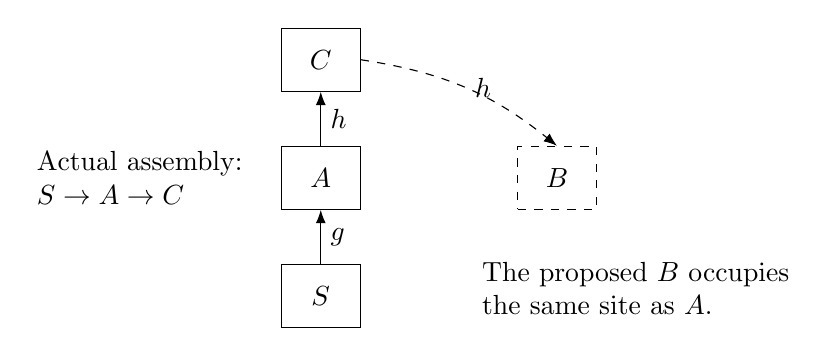
\begin{tikzpicture}[>=Latex,box/.style={draw,minimum width=1cm,minimum height=.8cm}]
\node[box] (s) at (0,0) {$S$};
\node[box] (a) at (0,1.5) {$A$};
\node[box] (c) at (0,3) {$C$};
\draw[->] (s)--node[right] {$g$} (a);
\draw[->] (a)--node[right] {$h$} (c);
\node[box,dashed] (b) at (3,1.5) {$B$};
\draw[->,dashed] (c.east) to[bend left=15] node[right] {$h$} (b.north);
\node[align=left] at (4.0,0.1) {The proposed $B$ occupies\\the same site as $A$.};
\node[align=left] at (-2.3,1.5) {Actual assembly:\\$S\to A\to C$};
\end{tikzpicture}
\caption{A later compatible bond is not a later available site. The dashed
step is valid only in the unsound relaxation.}
\end{figure}

This is a counterexample to a particular proposed simplification, not a
claimed defect in the existing repository's occupancy-aware compiler.
The package includes both a reduced three-rule instance and the literal
four-tile rule catalogue restricted to the three vertical sites.

\subsection{What directedness does permit}
Call a seeded system \emph{compatible} when every two finite producible
assemblies agree wherever both are defined. This standard confluence
property holds for directed aTAM systems in the usual setting.

\begin{lemma}[Compatible union]\label{qoc:ts:lem:union}
For nonnegative singleton attachments, the union of two compatible finite
producible assemblies is producible. The statement also holds when all
positions are restricted to a fixed box.
\end{lemma}
\begin{proof}
Build the first assembly. Follow a legal sequence for the second, skipping
tiles already present. A skipped tile has the same type by compatibility.
At each unskipped step all supporting tiles from the second sequence are
present, and extra tiles cannot decrease the bond sum. Thus every remaining
step is legal. No new position outside the two assemblies is used.
\end{proof}

\begin{writenote}
This is the union-closure step of \lab{cdc:of:prop:antimatroid} in \emph{Canonical Diophantine certificates}, Part~XI, with the same skip-already-present argument; the batch serialization of Section~\ref{qoc:ts:sec:selfassembly} is its \lab{cdc:of:lem:closure}.
\end{writenote}

\begin{corollary}[Boxwise uniqueness and monotone exhaustion]\label{qoc:ts:cor:box}
In a compatible system, every maximal finite-box assembly is the same.
The canonical unit-delay compiler produces it. For nested boxes
$B_1\subseteq B_2$ containing the seed, these maximal assemblies are
nested. Every finite producible assembly is contained in a sufficiently
large box outcome.
\end{corollary}
\begin{proof}
Two maximal assemblies in the same box have a producible union there;
maximality forces equality. A maximal assembly in $B_1$ and one in $B_2$
are compatible, and their union is producible in $B_2$, so maximality in
$B_2$ gives inclusion. Finally any finite producer fits in some box;
union with that box's maximal outcome and maximality give containment.
\end{proof}

The directedness claim here is not \emph{intrinsic universality}. There is
no implication that one directed two-dimensional system simulates the full
dynamics of every directed system. The impossibility result for directed
intrinsic universality is a different theorem \cite{ts:hendricks}.

\section{Timing regions, succinctness, and nonmonotonicity}
\subsection{Finite polyhedral timing semantics}
The event model also makes sense for strictly positive real delays.
Its integer polynomial representation is not being extended to all reals;
we study the semantic map separately in this subsection.

\begin{theorem}[Finite timing decomposition]\label{qoc:ts:thm:phases}
For a fixed catalogue and seed, the positive real delay orthant has a
finite partition into relatively open rational polyhedral cones such that
on each part the output labels and absent sites are constant. Every finite
activation time on a part is a homogeneous integer linear form
\[
 t_v=\sum_{e\in C_v}d_e
\]
with $C_v$ a set of distinct rules. In particular, the set of positive
integer delay vectors giving any prescribed label outcome is effectively
Presburger-definable and semilinear.
\end{theorem}
\begin{proof}
There are finitely many possible critical chains with distinct heads.
Each contributes a linear form with coefficients zero or one. Include
the zero form. By Lemma~\ref{qoc:ts:lem:bound}, whose strict-decrease proof also
works for positive real delays, every finite event time is one of these
forms. A currently enabled offer extends a critical chain to its vacant
head, again with distinct heads, so it too belongs to this finite family.

Take the central hyperplane arrangement obtained from equality of every
pair of these forms, and intersect all its relatively open faces with
the positive orthant. This is a finite rational polyhedral partition.
On each part every comparison between potential event times has a fixed
sign, including equality. Start with the fixed seed. The earliest enabled
time and the label tie rule consequently select the same sites and labels
throughout the part. Induction over at most $m$ successful site activations
shows that the whole event signature is fixed. Choosing a fixed critical
chain on each comparison face supplies the stated linear form for every
finite time.

All faces can be enumerated effectively from the catalogue, although
there can be many. Their integer points are described by integer linear
inequalities and equalities; strict inequalities can be replaced by the
corresponding one-unit inequalities on integer points. Taking the finite
union for a specified output yields an effective Presburger formula.
The classical equivalence between Presburger sets and semilinear sets
\cite{ts:ginsburg} gives
the last terminology; the explicit linear description is already enough
for our applications.
\end{proof}

\begin{writenote}
Second route for integer delays. Adding the query squares $(\ell_{v,a}-1)^2$ and $\ell_{v,a}^2$ (subsection ``Queries and changes of domain'') to the polynomial of Theorem~\ref{qoc:ts:thm:main} keeps the form~\eqref{qoc:ts:eq:form}; by Theorem \lab{cdc:of:thm:classification} of \emph{Canonical Diophantine certificates} ($\Dplus_2=\mathrm{SL}$), the set of integer delay vectors giving a prescribed label outcome is therefore semilinear. This recovers only the Presburger conclusion, not the real polyhedral partition or the linear forms of the theorem.
\end{writenote}

\begin{remark}[Where affine terms reappear]
Finite event times are homogeneous in the positive delay variables $d_e$.
The sentinel $1+\sum_e d_e$ is affine, not homogeneous. Rewriting
$d_e=1+\delta_e$ also turns the event-time forms into affine expressions
in $\delta_e$. There is no contradiction between these statements.
\end{remark}

\begin{corollary}[Common scaling]
Multiplying every delay by the same positive scalar preserves all output
labels and absent sites and scales every finite activation time by that
scalar. For positive integer scaling, the semantic part of the quadratic
certificate has this property, although its sentinel and auxiliary slacks
need not scale homogeneously.
\end{corollary}

\subsection{Why listing all regions can be exponentially wasteful}
\begin{theorem}[An exponential explicit-outcome lower bound]\label{qoc:ts:thm:exp}
There is a family of catalogues with $m$ sites and $2m$ empty-body rules
whose timing map has $2^m$ distinct label outcomes. Any representation
that explicitly lists separate constant-outcome regions needs at least
$2^m$ nonempty entries. The total quadratic compiler for this family uses
exactly $15m$ witnesses and $O(m)$ sparse monomials.
\end{theorem}
\begin{proof}
At site $i$, put two empty-body rules with labels 1 and 2 and delays
$x_i,y_i$. Label 1 wins exactly when $x_i\le y_i$; otherwise label 2 wins.
The independent choices $(x_i,y_i)=(1,2)$ or $(2,1)$ realize every label
vector. A region on which the outcome is constant cannot contain points
with two different vectors, so at least $2^m$ entries are necessary for
an explicit constant-outcome list. Here $q=2$, $D=L=0$, $R_0=R=2m$.
Equation~\eqref{qoc:ts:eq:W} gives $7m+6m+2m=15m$. The sparse bound follows
from Theorem~\ref{qoc:ts:thm:height}.
\end{proof}

This is an output-list lower bound, not a lower bound against every
symbolic representation. A decision diagram, a program, or the polynomial
can encode many outcomes without listing them. The theorem explains why
a compact Diophantine formulation may be more useful than an expanded
Presburger disjunction even when both define the same parameter set.

\subsection{Slowing one rule can accelerate a downstream event}
\begin{proposition}[Unbounded nonmonotone timing effect]\label{qoc:ts:prop:slowfast}
For a fixed exclusive-site catalogue, increasing one delay can make a
particular downstream activation arbitrarily many times faster, while
keeping that downstream label unchanged.
\end{proposition}
\begin{proof}
At site $p$, let empty-body rules offer labels $A$ and $B$ at times 2 and
3. A downstream site $x$ acquires its sole label from $p:A$ with delay
$K$, or from $p:B$ with delay 1. Initially $p$ chooses $A$, so $x$
activates at time $K+2$. Increase only the $A$ offer delay from 2 to 4.
Now $p$ chooses $B$ at time 3, and $x$ activates at time 4. The ratio
$(K+2)/4$ is unbounded as $K$ grows.
\end{proof}

Within a fixed critical-chain phase, finite times have nonnegative linear
coefficients. Globally, changing the winning label changes the available
rules, and monotonicity fails. Therefore a generic monotone min--max
sensitivity argument cannot be imported into the exclusive-label model
without checking the label phase. The example also distinguishes the
model from ordinary positive Horn closure, which has no such label race.

\section{Turing-complete substrates and the unbounded boundary}\label{qoc:ts:sec:boundary}
\subsection{An explicit positive Horn encoding of machine computation}
To make the computational boundary independent of an uninstantiated tile
set, we give a direct positive Horn encoding. Fix a deterministic Turing
machine with alphabet containing a blank symbol $\square$. Represent a
configuration by
\[
 C_q(L,a,R),
\]
where $q$ is the state, $a$ is the current symbol, and $L,R$ are finite
lists containing the tape symbols to the left and right, nearest first.
An empty list denotes an all-blank unrepresented tail. Lists use
constructors $\mathsf{nil}$ and $\mathsf{cons}$.

For a right-moving transition $(q,a)\mapsto(q',b,\mathrm{right})$, include
\begin{align*}
 \Reach(C_q(L,a,\mathsf{cons}(c,R)))
 &\Rightarrow\Reach(C_{q'}(\mathsf{cons}(b,L),c,R)),\\
 \Reach(C_q(L,a,\mathsf{nil}))
 &\Rightarrow\Reach(C_{q'}(\mathsf{cons}(b,L),\square,\mathsf{nil})).
\end{align*}
For a left-moving transition include
\begin{align*}
 \Reach(C_q(\mathsf{cons}(c,L),a,R))
 &\Rightarrow\Reach(C_{q'}(L,c,\mathsf{cons}(b,R))),\\
 \Reach(C_q(\mathsf{nil},a,R))
 &\Rightarrow\Reach(C_{q'}(\mathsf{nil},\square,\mathsf{cons}(b,R))).
\end{align*}
Stationary transitions, if used, simply replace $q,a$ by $q',b$.
For a halting state $h$, include
\[
 \Reach(C_h(L,a,R))\Rightarrow\Halt.
\]
The seed fact is the input configuration. Variables range over the
indicated constructor terms. All clauses are positive and every rule has
one body atom.

\begin{proposition}[Exact Horn simulation]\label{qoc:ts:prop:tmhorn}
The derived ground $\Reach$ atoms are exactly the machine configurations
on its run, and $\Halt$ is derivable exactly when that run halts. A fixed
universal machine therefore gives one fixed finite Horn program whose
halting derivability problem is computably enumerable complete.
\end{proposition}
\begin{proof}
Every ground transition clause performs exactly the designated tape
operation, including the empty-tail blank case. Induction on the length
of the run proves that every reached configuration is derivable.
Conversely, induction on a finite derivation shows that every newly
produced configuration is the prescribed successor of one already on
the run. The only clauses with head $\Halt$ have a halting configuration
as their premise. Fixing a universal machine and encoding a machine/input
pair in its initial tape gives the usual halting reduction.
\end{proof}

The representation is a Turing-complete computational substrate consisting
only of monotone accumulation of structured facts. No register decrement
or destructive rewrite is required; computational power comes from the
unbounded term universe.

\subsection{Every finite grounding has a total quadratic certificate}
Choose a size bound $b$ and enumerate a finite set of well-formed
configuration terms, for example all configurations whose two list lengths
sum to at most $b$, together with $\Halt$. Include only ground rule
instances all of whose atoms belong to this finite set. For sufficiently
large $b$ the initial configuration is included. This is a finite Horn
catalogue and Theorem~\ref{qoc:ts:thm:horn} applies.

Let $h_b\in\{0,1\}$ indicate whether $\Halt$ belongs to its closure.
The groundings may be chosen nested, so $h_b$ is nondecreasing. A finite
machine run uses only finitely many configurations of finite size. Thus
\begin{equation}\label{qoc:ts:eq:haltexhaustion}
 \text{machine halts}\quad\Longleftrightarrow\quad
 \exists b\; h_b=1.
\end{equation}
Each individual closure and its negative answer $h_b=0$ have unique
quadratic natural certificates. Grounding cost is explicit: the finite
universe can be exponentially large in its term-size bound. Neither
term enumeration nor the changing number of sites is free.

\begin{remark}[A three-witness presence flag]
The optimized Horn compiler records only a time. For a queried fact with
$0\le t\le M$, introduce $b,h,s\in\N$ and add
\[
 (b+h-1)^2+(M-t-b-s)^2+hs.
\]
Its unique zero has $b=1,h=0,s=M-t-1$ when $t<M$, and
$b=0,h=1,s=0$ when $t=M$. Indeed one-hotness forces $b,h$ to be
complementary Boolean values, and $hs=0$ distinguishes the zero gap
from a positive gap. Thus $b$ is precisely the truth flag, with three
additional witnesses and still total degree two. Fixing $b$ to zero or
one adds one affine square and no further witness. These three query
coordinates are additional to the unqueried Horn count.
\end{remark}

\subsection{Why permanent absence is not existentially compressible}
\begin{theorem}[Permanent-absence obstruction]\label{qoc:ts:thm:absence}
For the fixed universal Horn program in Proposition~\ref{qoc:ts:prop:tmhorn},
there is no single integer polynomial $Q(n,\boldsymbol z)$ such that,
for every valid coded input $n$,
\[
 \Halt\text{ is never derived on }n
 \quad\Longleftrightarrow\quad
 \exists\boldsymbol z\in\N^k\ Q(n,\boldsymbol z)=0,
\]
where $k$ is fixed. Nor is there a total computable function bounding a
sufficient accepting grounding size in terms of the encoded input length.
\end{theorem}
\begin{proof}
Existential natural zeros of any fixed integer polynomial can be
effectively enumerated, so such a $Q$ would make nonhalting computably
enumerable. Halting is also computably enumerable. Dovetailing the two
enumerations would decide halting, a contradiction.

Suppose a computable function $f$ guaranteed that every halting input of
length $n$ had $h_b=1$ for some $b\le f(n)$. Given an input, enumerate
those finitely many groundings and compute their finite closures. A
positive answer detects halting; exhaustion with no positive answer
detects nonhalting. This is the same contradiction. The argument works
for a bound depending computably on the entire input as well.
\end{proof}

\begin{corollary}[The size escapes every computable bound]
For every total computable function $f$, there is a halting input whose
least accepting grounding size exceeds $f$ of its input length. In fact
there are infinitely many such inputs.
\end{corollary}
\begin{proof}
If there were only finitely many exceptions, their finitely many minimal
accepting sizes would have a maximum $C$. The computable bound
$\max(f(n),C)$ would work for every halting input, contradicting the
previous theorem. This is an existence argument; it does not compute $C$.
\end{proof}

\begin{writenote}
The second half of Theorem~\ref{qoc:ts:thm:absence} is a case of \lab{cdc:bd:prop:nobound} of \emph{Canonical Diophantine certificates}, whose list of specializations already includes tile systems, and of its Part~XI form \lab{cdc:of:prop:nocutoff}.
\end{writenote}

Equivalently, permanent absence is the universal statement
$\forall b\ h_b=0$, not one more finite closure query. Arithmetic coding
can replace a changing-length witness by a finite sequence code, but
preserving polynomial degree, fixed arity, and uniqueness through that
coding is a separate theorem that has not been supplied here. The general
single-fold or finite-fold Diophantine problem is not resolved by having a
single-fold polynomial for every fixed finite size \cite{ts:matiyasevich}.

\subsection{The same boundary in algorithmic self-assembly}
Classical tile constructions simulate computation \cite{ts:winfree}. On any
fixed directed universal computational tile construction with a suitable
finite input seed and a designated halting output, Corollary~\ref{qoc:ts:cor:box}
gives the geometric counterpart of \eqref{qoc:ts:eq:haltexhaustion}: a halting
tile occurs exactly when it occurs in some finite-box outcome. Every box
has the total quadratic certificate of Section~\ref{qoc:ts:sec:selfassembly}.\footnote{\wtag\ Source~12 wrote ``Section~7'', its own number for this section.} Nonoccurrence in
\emph{every} box is again a universal condition; a fixed existential
polynomial for all nonhalting inputs would contradict the same
computability argument.

The artifact does not instantiate a new universal numerical tile alphabet.
Its literal tile example is the four-type occupancy counterexample. The
universal Horn reduction is explicit above, while the aTAM universality
transfer uses the classical computational substrate theorem. This keeps
semantic correctness separate from a numerical universal compiler claim.

\section{Implementation, exported polynomials, and tests}\label{qoc:ts:sec:impl}
\subsection{What the package actually implements}
The file \code{code/quadratic_compiler.py} is a standard-library Python
implementation using exact integers. It contains an event simulator, a
sparse affine-expression class, the total exclusive-site compiler, an
optimized Horn compiler, a canonical witness constructor, and an expanded
polynomial exporter. No floating-point arithmetic, numerical optimization,
or symbolic-system black box is used.

\begin{writenote}
In this report the programs are \path{code/12-total-quadratic-quadratic_compiler.py}, \path{code/12-total-quadratic-test_compiler.py} and \path{code/12-total-quadratic-verify_exports.py}, and every file of \path{results/} is \path{data/12-total-quadratic-*}. The test program rewrites its receipt and the four example files in place: run it only on a copy in the delivered layout (README). It was rerun at placement with Python~3.14.4: all checks passed, the four examples were reproduced apart from line endings, and the receipt differed only in its run time. The research programme's review found that the compiler keeps references to its mutable inputs, returns aliased export lists and accepts a fractional seed label; its patch \path{total_quadratic_immutable_inputs.patch} changes no valid polynomial. The shipped file is unpatched.
\end{writenote}

The polynomial exporter retains both the structured penalty description
and a fully expanded sparse monomial list. A monomial is represented by
its integer coefficient and zero, one, or two variable names. All variable
names, delay parameters, and a complete zero assignment are included in
each exported example. The JSON representation is an explicit polynomial,
not merely pseudocode for an unspecified arithmetic relation.

A separate \code{code/verify_exports.py} reconstructs each exported
polynomial from its penalty data without importing the compiler, checks
exact equality with the sparse monomial list, and verifies the supplied
zero and that all of its coordinates are natural numbers.

The executable compiler accepts a fixed site count, label count, seed,
and catalogue. It rejects repeated seed sites, invalid literals, rules
whose heads are already seeded, duplicate body literals, and nonpositive
or wrongly sized delay lists. Rules for seeded heads can be removed
semantically before compilation; rejecting them keeps the interface
unambiguous.

\subsection{Examples and exact counts}
\begin{center}\small
\begin{tabular}{lrrrrr}
\toprule
Example & Parameters & Witnesses & Squares & Products & Monomials\\\midrule
Reduced locking example & 0 & 29 & 18 & 13 & 126\\
Literal four-tile example & 0 & 58 & 36 & 27 & 302\\
Timed race and blocked cycle & 8 & 85 & 56 & 35 & 435\\
Four-rule huge-delay chain & 4 & 45 & 30 & 18 & 206\\\bottomrule
\end{tabular}
\end{center}
All four expanded polynomials have total degree two. Their complete
assignments evaluate to zero in exact arithmetic.

The huge-delay chain has four delays
\[
 10^{30}+1,\quad10^{30}+3,\quad10^{30}+7,\quad10^{30}+9.
\]
Its four nonseed activation times are respectively
\[
 10^{30}+1,\quad2\cdot10^{30}+4,\quad
 3\cdot10^{30}+11,\quad4\cdot10^{30}+20.
\]
The largest witness needs 103 bits, but the compiler still allocates 45
witnesses and 206 expanded monomials. The values of the parameters change;
the polynomial does not. This is a direct demonstration of delay-uniform
size rather than a benchmark against an optimized time-unrolled compiler.

In the timed-race example the output labels are $[1,1,1,0,0,2]$ and the
finite times are $0,2,5,9$ at sites $0,1,2,5$; sites 3 and 4 form an
unseeded blocked cycle. Equal-time offers of labels 1 and 2 at site 1
select label 1. All these values are recorded in the exported JSON.

\subsection{Finite verification receipts}
Running
\begin{verbatim}
python code/test_compiler.py
\end{verbatim}
regenerates the examples and \code{results/test_receipt.json}. The recorded
run passed the following checks.
\begin{center}\small
\begin{tabular}{lr}
\toprule
Check & Count\\\midrule
Min/max gate assignments examined & 15,552\\
Typed effective-time assignments examined & 5,868\\
Complete semantic assignments enumerated & 68,885\\
Instances with exactly one enumerated semantic fixed point & 1,059\\
General compiled instances checked & 1,663\\
Single-coordinate witness mutations rejected & 33,574\\
Expanded-polynomial evaluations compared with penalties & 216\\
Reproducible random catalogues & 300\\
Distinct outputs of the eight-site timing family & 256\\
Four-neighbor weight/threshold policies checked & 3,072\\
Optimized Horn/general compiler comparisons & 320\\
Malformed inputs rejected & 7\\\bottomrule
\end{tabular}
\end{center}

The semantic enumeration includes \emph{all} subsets of the eight Horn
rules on two unseeded one-label sites with arbitrary subset bodies. It
also includes every catalogue of at most two distinct rules on two
unseeded two-label sites with empty or singleton bodies, with every
assignment of delays from $\{1,2\}$. It enumerates candidate active time
zero as well as positive times, so unsupported zero-time fixed points
would not be missed.

Random tests use seed 20261002 and include incompatible labels in a body,
self-dependencies, cycles, empty bodies, no-rule heads, and partly or
fully seeded systems. A separate deliberate zero-delay self-rule exhibits
the predicted two fixed points outside the model. An independent sparse
monomial evaluator is compared against the structured penalty evaluator
both at the intended zero and at off-zero natural tuples.

The mutation check changes one witness by $+1$ while keeping all other
coordinates fixed. Rejecting all such changes is a useful sensitivity
test, but is not a proof of global uniqueness. The unrestricted uniqueness
claim rests on Theorems~\ref{qoc:ts:thm:fixedpoint} and \ref{qoc:ts:thm:main}; the
finite enumerations and mutations are regression tests. Likewise, the
threshold enumeration supports but does not replace the antichain proof.

\section{Integration into ProveIt}
The main formalization target is small enough to isolate from a universal
Diophantine backend. A natural dependency sequence is:
\begin{enumerate}[label=\arabic*.]
\item Define the finite catalogue, immutable seed, and event semantics.
Prove strict causal dependence and the critical-chain bound without any
polynomial syntax.
\item Define the capped output equations. Prove existence and uniqueness
by the time-induction argument, explicitly distinguishing absence from
an unproved high-rank event.
\item Prove the natural-number min/max, typed-prerequisite, and integer-key
winner lemmas. Include the hypotheses $q\ge1$, positive delays, and
natural domains in the theorem statements.
\item Build an affine-penalty syntax with a theorem that every emitted
product has nonnegative factors. Prove the zero-set equivalence between
the assembled polynomial and its semantic equations.
\item Connect the list-based allocator to exact counts and an executable
witness constructor. Only then connect to a general Diophantine predicate
interface and add finite-box self-assembly adapters.
\end{enumerate}
The Python compiler is not a trusted proof certificate until such a
checker theorem is proved. Conversely, no large numerical solver should
need to be trusted: the emitted polynomial and the witness can be evaluated
by exact arithmetic, while the all-input soundness argument is structural.

A useful interface should expose four different theorems rather than one
ambiguous ``compiler correctness'' statement: exact outcome decoding,
existence for every legal delay vector, uniqueness of all auxiliaries,
and the domain/size ledger. Optimizations can then specify whether they
preserve the same tuples, provide a bijective coordinate change, or only
preserve the outer accepted-input relation. The repository already treats
such distinctions carefully in its research ledgers
\cite{ts:repo-h10,ts:repo-native}; this compiler should preserve that discipline.

\section{Further research questions}\label{qoc:ts:sec:future}
\subsection{Verified allocation and sharing}
Can the exact witness formulas be proved together with a verified sparse
polynomial generator in Lean? The highest-value first targets are the
symbolic-cap selector and the winner lemma, because they protect against
accidental quartic degree growth and inactive-branch multiplicity. A
subsequent optimization should share identical maxima and repeated
head offers while proving a full zero-set bijection, not merely counting
fewer printed operations.

\subsection{Smaller exclusive-label interfaces}
The current allocation spends $2q+3$ site coordinates plus typed-literal
selectors. Can a binary label representation reduce dependence on $q$
without introducing ambiguous comparison witnesses or increasing degree?
The integer-key construction avoids one selector per rule, but a binary
encoding requires exact equality-to-label tests. A useful answer must
report coefficient sizes, monomial counts, and complete witness
multiplicity, not only the number of semantic bits.

\subsection{Parametric support selection}
Here the topology and sufficient-support catalogue are fixed. For
self-assembly, glue strengths and temperature are compiled into that
catalogue before the polynomial is emitted. Can one make these values
uniform numerical parameters, retain one natural root, and avoid
exponentially enumerating support choices as neighborhood degree grows?
For four neighbors the finite enumeration is harmless; unbounded fan-in
requires a genuinely different mechanism.

\subsection{All nondeterministic outcomes rather than one eager outcome}
The present total compiler chooses a deterministic label-priority timing
semantics. Representing all asynchronous terminal outcomes exactly once
requires quotienting away attachment order without discarding causal
competition. Existing order-free assembly work is the relevant starting
point, not an assumption that our eager outcome enumerates all outcomes.
A desirable theorem would count one zero per final assembly and specify
how timing feasibility interacts with that quotient.

\begin{writenote}
The existing order-free work is Part~XI of \emph{Canonical Diophantine certificates}, whose convex compiler has one natural zero per producible labelled target (\lab{cdc:of:thm:compiler}) and a whole-grid terminality extension (\lab{cdc:of:thm:terminal}). What this question adds is the interaction with timing.
\end{writenote}

\subsection{The sharp zero-delay and inhibition boundary}
Zero delays create unsupported cyclic fixed points. One possible repair
is to separate physical time from a strictly increasing causal rank.
Can rank normalization be made unique without paying for a history?
Negative glues and inhibitors are harder: a body can cease being enabled,
so pending offers matter. Identify a maximal nonmonotone extension in
which a finite outcome still determines a canonical compact certificate.
Counterexamples should distinguish failed abstractions from impossible
representations in principle.

\subsection{Timing geometry without enumerating every phase}
The phase theorem is constructive but its explicit list can be
exponential. Can one compute a compact decision structure for a queried
output, or certify robustness on an entire delay polytope, without
expanding every phase? The slowdown/acceleration example shows that
coordinatewise monotonicity cannot be assumed. A precise target is a
certificate that a fixed output persists throughout a specified rational
box of positive delays, with sharp complexity bounds.

\subsection{Canonical small obstructions to finite activation}
A false fact in a finite Horn closure is certified here by the entire
unique rank vector. Is there a canonical minimal blocking object that
can be smaller, while admitting a polynomial-time, unique-witness
arithmetic description? Minimal cuts need not be unique, and choosing
the lexicographically first cut can hide additional verification work.
The useful objective is a provable size--height trade-off with an exact
uniqueness theorem.

\subsection{From finite boxes to fixed arity}
For universal Horn computation, the finite-size hierarchy is explicit,
and the least accepting size outruns every computable bound. What
structure of a restricted class permits fixed-arity compression of this
hierarchy while preserving finite or single fold? Candidate restrictions
include bounded treewidth of dependency supports, ultimately periodic
space use, and a fixed finite set of critical-chain shapes. Such results
would need a new coding theorem; they cannot follow from writing
$\exists b$ before a family of different polynomials.

\subsection{Literal universal tile compilation}
A concrete integration project is to choose a published directed
computationally universal tile construction, freeze its exact numerical
alphabet and input encoding, and run the finite-box compiler on it.
This would replace the current classical aTAM transfer by an audited
end-to-end implementation. It should not be confused with a directed
intrinsic-universal simulator, whose stronger two-dimensional requirement
has a known obstruction \cite{ts:hendricks}.

\section{Conclusion}
The central result is a total quadratic semantics, not merely an
existential encoding of successful traces. Positive delays enforce
causality; a finite sentinel handles absence; typed effective-time gates
preserve exclusive occupancy; and integer winner keys remove tie
multiplicity. These ingredients give an exact, delay-uniform allocation
and one complete natural zero for every finite input instance.

The applications illustrate two complementary facts. Irreversible
substrates can compute universally through an unbounded supply of sites
or structured facts, while every fixed finite restriction can have an
extremely rigid low-degree certificate. The difference between these
statements is where the unbounded computational difficulty resides.
The supplied proofs and executable sparse polynomials establish the
finite side explicitly and identify, rather than conceal, the obstacle
to universal negative or fixed-arity single-fold compression.


\clearpage
\part{Quadratic Diophantine certificates for a fixed Waterfall universal machine}\label{qoc:part:wf}

\begin{writenote}
Part~\ref{qoc:part:wf} prints source~14 (batch-78 manuscript~14). Its Section~$n$ is Section~$n+29$ here (Sections~\ref{qoc:wf:sec:results}--38), and its Theorem~$n.m$ is Theorem~$(n+29).m$; its appendices A--B are Appendices~\ref{qoc:wf:app:matrix}--\ref{qoc:wf:app:gaps}. Source~14 names no repository commit and did not consult the repository; the repository material it bears on is added in \wtag\ notes (Sections~\ref{qoc:wf:sec:substrate}, \ref{qoc:wf:sec:example}, \ref{qoc:wf:sec:scope} and~\ref{qoc:wf:sec:obstruction}).
\end{writenote}

\begin{center}
{\large\bfseries Quadratic Diophantine certificates for a fixed Waterfall universal machine}\\[3pt]
{\small Research note prepared with AI assistance. 2 October 2026.}
\end{center}

\begin{writenote}
The delivered author line adds ``for private review''; this public report prints it in Appendix~\ref{qoc:app:provenance} only.
\end{writenote}

\begin{abstract}
A fixed 46-clock Waterfall program due to Iijil simulates the binary 15-state universal Turing machine of Neary and Woods. We give an explicit two-half-tape input interface, prove its complete macrostep behavior by a finite exact affine certificate, and compile an externally fixed number $k$ of Turing-machine steps into one quadratic Diophantine equation. The equation has exactly $35k$ natural witnesses, $5k+4$ squared linear residuals, and $2k$ nonnegative complementarity terms. Its natural fiber is empty or a singleton and records both the exact prehalt clock-firing count and the physical halt timestamp. The certificate eliminates every repetition internal to a Waterfall macrostep, including repetitions exponential in input bit length. A separate decidable common-column class admits horizon-free certificates. All scope distinctions are explicit: the universal machine is prior work, the witness dimension grows with $k$, and no fixed-arity representation of unbounded universal computation or universal arithmetic-operation record is claimed. An exact-integer replay package accompanies the note.
\end{abstract}
\section{Results and scope}\label{qoc:wf:sec:results}
The Waterfall Model is an esoteric counter substrate in which all counters decrease together and a counter reaching zero applies a fixed nonnegative increment vector. Its lack of an instruction pointer makes its event sequence an interesting arithmetic object. The direct question here is whether its long runs admit explicit Diophantine certificates that exploit the substrate's structure rather than merely recording every event.

The main result is a \emph{bounded-macrostep} answer. The fixed machine, its Turing-machine source, and the compiler from which it comes are prior work of Iijil~\cite{wf:iijil-matrix,wf:iijil-tm,wf:iijil-compiler}; the underlying universal Turing machine is due to Neary and Woods~\cite{wf:nw}. The contribution of this note is the explicit input contract and its symbolic verification, the compressed arithmetic certificates, and the proofs and replay artifacts tying them together. Priority of this particular arithmetic presentation has not been established by an exhaustive literature search.

Throughout, $\N=\{0,1,2,\ldots\}$. State labels $A,\ldots,O$ have numeric codes $0,\ldots,14$. The head symbol has code $0$ or $1$. The finite-support half tapes, read away from the head with least significant digit first, are natural integers $L,R$; the current head symbol is stored separately.

\begin{theorem}[Main result]\label{qoc:wf:thm:main}
There is a fixed $46\times46$ nonnegative integer Waterfall increment matrix $M$, with entries at most $12$, and an explicitly given canonical initial vector $\cani(A,0,L,R)$ with the following properties.
\begin{enumerate}[label=(\roman*)]
\item Every $L,R\in\N$ gives a tie-free run up to and including its possible halt. The program exactly simulates the Neary--Woods $15$-state binary machine, with both half tapes supplied as raw integers. Computing its two varying clock values takes four binary arithmetic operations.
\item A Turing-machine step that pops $X=2Q+r$, $r\in\{0,1\}$, and pushes onto half tape $Y$ uses exactly
\[
 c=6+3Q+r+3Y
\]
nonhalting Waterfall firings. Consecutive transition-event timestamps differ by $2c+7$.
\item For every externally fixed $k\ge1$, an explicitly constructible integer polynomial
\[
 F_k(L_0,R_0,C,\tau;\mathbf z),\qquad \mathbf z\in\N^{35k},
\]
of total degree two vanishes exactly when this run first halts after $k$ Turing-machine steps, after $C$ nonhalting Waterfall firings, at timestamp $\tau$. For fixed parameters, there is at most one natural witness tuple.
\end{enumerate}
\end{theorem}

The numerical size of a tape value does not increase the number of macrostep witnesses. The number of Turing-machine steps does: $k$ is compiler data specifying a polynomial and its arity, not one more quantified variable in a fixed polynomial. This distinction is central. In particular, the theorem does not supply a universal fixed-arity quadratic Diophantine equation.

The note first fixes the semantics and complete machine data, then proves the macrostep and arithmetic theorems. Section~\ref{qoc:wf:sec:scope} explains the finite-horizon and semilinearity boundaries. Section~\ref{qoc:wf:sec:common} treats a different, decidable family where a genuinely horizon-free certificate is available. Appendix~\ref{qoc:wf:app:matrix} specifies every matrix entry compactly; Appendix~\ref{qoc:wf:app:gaps} records the finite affine certificate behind the all-input proof.

\section{The fixed substrate and its input contract}\label{qoc:wf:sec:substrate}
\subsection{Deadlines and strict minimum semantics}
There are $n$ actual clocks, indexed by $i$, and one distinguished halt clock $h$. The column $M_{\cdot i}$ is the increment vector for firing clock $i$. Assume $M_{ji}\ge0$, $M_{ii}>0$ for $i\ne h$, and $M_{\cdot h}=0$. Starting from an integer vector $a>0$, let $p_i$ count previous nonhalting firings. Define the vector of absolute deadlines by
\begin{equation}\label{qoc:wf:eq:deadlines}
 d=a+Mp.
\end{equation}
The next event is the unique minimum coordinate of $d$. A minimum tie is undefined. When that coordinate is $h$, the computation halts \emph{before} any update. Otherwise increment $p_i$ by one, equivalently adding $M_{\cdot i}$ to $d$.

This is the integer version of the standard simultaneous-decrement semantics~\cite{wf:waterfall}. Indeed, at physical time $t$ with current clock values $v_i$, each deadline is $t+v_i$. Advancing time to the first zero changes neither deadline; adding a trigger vector changes deadlines by that same vector. Induction proves~\eqref{qoc:wf:eq:deadlines}. After a legal nonhalting event the selected deadline strictly increases, all others are still larger than the old minimum, and no deadline decreases. Thus successive event times are strictly increasing integers; infinitely many events cannot accumulate in finite time. We keep physical timestamps even though an implementation may accelerate idle intervals.

The source file uses the opposite matrix orientation: each trigger is a \emph{row}. It has 47 rows and columns because the first row and column carry serialization metadata and initial values. The mathematical matrix $M$ is the transpose of its $46\times46$ trigger submatrix. The metadata coordinate is never treated as a clock here.

\subsection{Clock names and the source machine}
For each direction $D\in\{L,R\}$ there are eight auxiliary clocks:
\[
 D\clk{Tape},\ D\clk{Temp},\ D\clk{Trans},\ D\clk{Div}_0,\ D\clk{Div}_1,
 \ D\clk{Mult},\ D\clk{Write}_0,\ D\clk{Write}_1.
\]
There are also thirty control clocks $\clk{Trans}_{q,s}$, one for each state-symbol pair. These are distinct from the two auxiliary clocks $D\clk{Trans}$. Their total is $16+30=46$.

Table~\ref{qoc:wf:tab:tm} gives the complete source transition function. An entry $(w,D,q')$ means write $w$, move in direction $D$, and enter state $q'$. The sole missing instruction is $(J,1)$; its clock, one-based number 28 in the source order, is the halt clock. The matrix and its complete compact definition in Appendix~\ref{qoc:wf:app:matrix} agree in all $2{,}116$ entries.

\begin{table}[htbp]
\centering
\caption{The fixed source machine. State codes run from $A=0$ to $O=14$.}\label{qoc:wf:tab:tm}
\begin{tabular}{@{}c cc @{
\qquad}c cc@{}}
\toprule
State & Read $0$ & Read $1$ & State & Read $0$ & Read $1$\\\midrule
$A$ & $(0,R,B)$ & $(1,R,A)$ & $I$ & $(0,R,A)$ & $(1,L,J)$\\
$B$ & $(1,R,C)$ & $(1,R,A)$ & $J$ & $(1,L,K)$ & undefined\\
$C$ & $(0,L,G)$ & $(0,L,E)$ & $K$ & $(0,R,L)$ & $(1,R,N)$\\
$D$ & $(0,L,F)$ & $(1,L,E)$ & $L$ & $(0,R,M)$ & $(1,R,L)$\\
$E$ & $(1,R,A)$ & $(1,L,D)$ & $M$ & $(0,L,B)$ & $(1,R,L)$\\
$F$ & $(1,L,D)$ & $(1,L,D)$ & $N$ & $(0,L,C)$ & $(0,R,O)$\\
$G$ & $(0,L,H)$ & $(1,L,G)$ & $O$ & $(0,R,N)$ & $(1,R,N)$\\
$H$ & $(1,L,I)$ & $(1,L,G)$ & & &\\\bottomrule
\end{tabular}
\end{table}

In Neary--Woods notation, $u_1,\ldots,u_{15}$ correspond to $A,\ldots,O$ and $c,b$ to $0,1$. The table is Table~16 on PDF page~17 of the author-hosted primary paper. Its missing $(u_{10},b)$ transition agrees with the final displayed halting configuration on PDF page~19. The following prose instead says $c$, a local inconsistency resolved here in favor of the table and displayed configuration. In particular, the $u_{15},b$ target is $u_{14}$, as in the primary table.

\begin{writenote}
The repository's research note \path{Computability/HilbertTenthProblem/Papers/research-wip/native-stream-queue/neary_woods_explicit_universal_tm.md}, added on 1~October 2026, a day before source~14, transcribes the same Table~16 for its own universal polynomial and reports the same inconsistency between Table~16's missing $(u_{10},b)$ and the prose of Neary and Woods's Section~3.5. Table~\ref{qoc:wf:tab:tm} agrees with that transcription entry by entry (states $u_i\mapsto$ the $i$th letter, $c\mapsto0$, $b\mapsto1$). Source~14 did not know the note; the erratum is printed once, here, and the two transcriptions were made independently.
\end{writenote}

\subsection{Canonical states and a four-operation loader}
Define a vector $\cani(q,s,L,R)$ of normalized deadlines by
\begin{align}
 \cani_{L\clk{Tape}}&=2+2L,& \cani_{R\clk{Tape}}&=2+2R,\label{qoc:wf:eq:canon-tapes}\\
 \cani_{D\clk{Div}_j}&=2+\ind{j\ne s},&&D\in\{L,R\},\ j\in\{0,1\},\label{qoc:wf:eq:canon-div}\\
 \cani_{\clk{Trans}_{u,t}}&=1+\ind{u\ne q}+\ind{t\ne s}.\label{qoc:wf:eq:canon-control}
\end{align}
Every other coordinate is $2$. Exactly one coordinate has value $1$, namely the next control clock $\clk{Trans}_{q,s}$.

The universal initial condition is $q=A,s=0$. All initial values except the two in~\eqref{qoc:wf:eq:canon-tapes} are fixed. Loading raw $L,R$ therefore costs two multiplications by the fixed constant $2$ and two additions: four operations in the binary $+,-,\times$ model, where constants and copying are free. This is a statement about the \emph{interface}, not the cost of encoding an arbitrary external program convention as $L,R$.

If a syntactically valid source serialization is desired, set its upper-left metadata bound to
\[
 H_{\rm file}=2(L+R)+47=(2+2L)+(2+2R)+43.
\]
It is strictly larger than every actual initial value, every trigger increment, and the metadata clock count $46$. Two further additions suffice. Thus the operational loader has four operations and the full serialization loader has six.

The primary paper starts its universal machine in $u_1$ over the rightmost $c$ of $bc$, with the encoded program to the left. Allowing \emph{both} half tapes is therefore part of the input contract. Its finite input encoding yields such natural $L,R$ effectively. Combining that universality result with the exact simulation proved below shows that halting on this fixed Waterfall matrix, as a set of pairs $(L,R)$, is computably enumerable complete. No small arithmetic cost is asserted for the separate program-to-half-tape encoding.

\section{An exact macrostep theorem}\label{qoc:wf:sec:macro}
A \emph{canonical cut} is a deadline vector $\cani(q,s,L,R)+t\one$ just before the next control-clock event; its event timestamp is $t+1$. We also use this vector identity immediately after the last trigger of the preceding macrostep, when an idle interval can remain before that event.

\begin{theorem}[Complete macrostep]\label{qoc:wf:thm:macro}
Suppose $(q,s)\mapsto(w,D,q')$ is defined in Table~\ref{qoc:wf:tab:tm}. Let $O$ denote the opposite direction, $X$ the half tape in direction $D$, and $Y$ the other half tape. Write $X=2Q+r$, with $Q\in\N$ and $r\in\{0,1\}$. Starting at $\cani(q,s,L,R)$, the exact firing word before the next control-clock event is
\begin{equation}\label{qoc:wf:eq:macro-word}
\begin{split}
 &\clk{Trans}_{q,s}\,
 (D\clk{Div}_0\ D\clk{Div}_1)^Q\,
 (D\clk{Div}_0)^r\,
 D\clk{Tape}\,
 (D\clk{Trans})^Q\,
 D\clk{Temp}\\
 &\hspace{1em}(O\clk{Mult})^Y\,
 O\clk{Tape}\,
 (O\clk{Trans})^{2Y}\,
 O\clk{Temp}\,
 O\clk{Write}_{w}.
\end{split}
\end{equation}
Every selected clock is the unique minimum. The final deadline vector is
\begin{equation}\label{qoc:wf:eq:macro-identity}
 \cani(q',r,L',R')+\Delta\one,
 \qquad \Delta=19+6Q+2r+6Y,
\end{equation}
where the popped half becomes $Q$ and the pushed half becomes $2Y+w$. The word has length
\begin{equation}\label{qoc:wf:eq:cstep}
 c=6+3Q+r+3Y,\qquad \Delta=2c+7.
\end{equation}
Zero exponents in~\eqref{qoc:wf:eq:macro-word} mean that the corresponding block is absent.
\end{theorem}

\subsection{A finite proof that covers unbounded tape values}
The only unbounded quantities in one macrostep are $Q$ and $Y$. Their loop repetitions can be certified by affine inequalities, without enumerating their possible values.

\begin{lemma}[Every-prefix endpoint criterion]\label{qoc:wf:lem:endpoint}
Let $v$ be the clock-count vector of a fixed finite word $w$, and let $u$ be the count vector of the prefix before one specified letter $i$ of that word. Before that letter in repetition $\ell$ of $w$, the gap between competitor $j$ and selected clock $i$ is
\begin{equation}\label{qoc:wf:eq:gap}
 d_j-d_i+(Mu)_j-(Mu)_i
   +\ell\big((Mv)_j-(Mv)_i\big).
\end{equation}
For $K\ge1$, the repeated word $w^K$ is a legal strict-minimum firing word if and only if, for every prefix position and every $j\ne i$, expression~\eqref{qoc:wf:eq:gap} is positive at $\ell=0$ and $\ell=K-1$.
\end{lemma}
\begin{proof}
A prescribed prefix determines its deadline vector by~\eqref{qoc:wf:eq:deadlines}, whether or not it is legal. Expression~\eqref{qoc:wf:eq:gap} is its exact deadline difference. A real affine function of $\ell$ attains its minimum on $[0,K-1]$ at an endpoint. Thus positivity of both endpoint values is equivalent to positivity at every integer iteration. Applying the criterion successively to every letter proves legality. Conversely, a legal repeated word necessarily passes its first- and last-iteration inequalities.
\end{proof}

It is important that the criterion is applied at \emph{every prefix position of each repeated block}. Checking only the beginning and end of a whole computation is insufficient; Section~\ref{qoc:wf:sec:obstruction} gives an explicit counterexample to that different shortcut.

\begin{proof}[Proof of Theorem~\ref{qoc:wf:thm:macro}]
Fix one of the 29 defined instructions and one of the two values of $r$. Substitute $X=2Q+r$ and the appropriate placement of $X,Y$ into the canonical vector. Process the blocks of~\eqref{qoc:wf:eq:macro-word} in order, adding the appropriate repeated trigger vectors to the deadline vector.

For a one-letter nonrepeated block, check all 45 competing clocks directly. For a block repeated $Q$ times, apply Lemma~\ref{qoc:wf:lem:endpoint} on its active domain $Q\ge1$; the zero case contributes no event. Similarly, use $Y\ge1$ for blocks repeated $Y$ or $2Y$ times. Every endpoint gap has the exact form
\[
 c+aQ+bY.
\]
After substituting $Q=Q_{\min}+q$ and $Y=Y_{\min}+y$, where the active-domain lower bounds are $0$ or $1$, each gap has a positive integer constant and nonnegative coefficients of $q,y$. Consequently every selected clock is uniquely minimal on the entire relevant natural domain.

For full reproducibility, the verifier checks 58 instruction-residue cases and 43,065 strict-minimum inequalities. There are 64 distinct affine forms when their active domains are retained; Appendix~\ref{qoc:wf:app:gaps} records this finite certificate. The source code uses coefficient tuples and exact integers, and its final check subtracts the proposed target in~\eqref{qoc:wf:eq:macro-identity} from \emph{all 46 coordinates}. Every residual coefficient is zero. This supplies an explicit finite algebraic verification of the stated identity, rather than extrapolation from a finite input grid.

Finally, counting letters gives $1+2Q+r+1+Q+1+Y+1+2Y+1+1=6+3Q+r+3Y$. The verified common shift is $19+6Q+2r+6Y=2c+7$.
\end{proof}

A second implementation establishes the loop inequalities by a different parameterization: for an iteration $j<Q$ use $Q=j+1+u$; for $j<Y$ use $Y=j+1+u$; for $j<2Y$ split $j=2v+e$, $e\in\{0,1\}$, and use $Y=v+1+u$. It proves nonnegativity of the resulting free-variable coefficients. This is an independent exact replay, not a proof-assistant formalization.

\subsection{Halting time and an independent linear potential}
The new canonical vector in~\eqref{qoc:wf:eq:macro-identity} has its next control event at $1+\Delta$. Thus $\Delta$ is a difference between \emph{consecutive control-event timestamps}, not necessarily the time elapsed to the immediately post-write state. For instance, from $L=R=0$ the first control event is at time $1$, its final write is at time $10$, and the next control event is at time $20$.

\begin{corollary}\label{qoc:wf:cor:time}
If the source machine first halts after $k$ executed instructions and the Waterfall run has made $C$ nonhalting firings, its halt timestamp is
\begin{equation}\label{qoc:wf:eq:tau}
 \tau=1+2C+7k.
\end{equation}
The final observation of the halt clock is not included in $C$.
\end{corollary}
\begin{proof}
The initial control event has timestamp $1$. Apply Theorem~\ref{qoc:wf:thm:macro} successively; each macrostep ends at a canonical cut with exactly the source-machine successor. Summing~\eqref{qoc:wf:eq:cstep} gives~\eqref{qoc:wf:eq:tau}. At $(J,1)$ the next unique minimum is the zero-trigger halt clock, so no additional update occurs.
\end{proof}

There is also a concise invariant checking the timing coefficients independently of the gap inequalities. Give the coordinates integer weights
\begin{equation}\label{qoc:wf:eq:weights}
 \omega_i=\begin{cases}
 288,&i=L\clk{Trans}\text{ or }R\clk{Trans},\\
 -373,&i\text{ is a division clock},\\
 970,&i\text{ is a multiplication clock},\\
 -4,&i\text{ is a write clock},\\
 0,&\text{otherwise}.
 \end{cases}
\end{equation}
Direct substitution in Appendix~\ref{qoc:wf:app:matrix} gives
\begin{align}
 \omega\cdot\one&=1008,&
 \omega\cdot\cani(q,s,L,R)&=1270,\label{qoc:wf:eq:potential-canon}\\
 \omega\cdot M_{\cdot i}&=2016+7056\ind{i\text{ is a nonhalt control clock}}
 &&(i\ne h).\label{qoc:wf:eq:potential-triggers}
\end{align}
The halt column has dot product zero. A prefix with $C$ firings and $k$ control firings therefore increases the potential by $2016C+7056k$. If its endpoints are canonical vectors differing by common shift $t$,~\eqref{qoc:wf:eq:potential-canon} makes that increase $1008t$. Hence $t=2C+7k$. This proves the same accounting identity; it does not by itself prove that a proposed event word is legal.

\section{One quadratic equation for an exact TM horizon}\label{qoc:wf:sec:quadratic}
We now use the macrostep semantics to eliminate all its internal repetition counts from the event-level trace. Fix $k\ge1$. The four supplied parameters are $L_0,R_0,C,\tau\in\N$. They are not counted as witnesses.

\subsection{Variables and linear expressions}
Let $\rulei$ be the set of the 29 defined instructions in Table~\ref{qoc:wf:tab:tm}. Write instruction $i$ as $(a_i,s_i)\mapsto(w_i,D_i,b_i)$, using numeric state codes. At each step $j=0,\ldots,k-1$, introduce 29 natural selectors $e_{ji}$ and six natural direction-group variables
\[
 Q_{jL},r_{jL},Y_{jL},\qquad Q_{jR},r_{jR},Y_{jR}.
\]
There are exactly $35k$ witnesses. Define the following \emph{linear expressions}, which introduce no further variables:
\begin{align}
 A_j&=\sum_{i\in\rulei}a_i e_{ji},& S_j&=\sum_{i\in\rulei}s_i e_{ji},& B_j&=\sum_{i\in\rulei}b_i e_{ji},\label{qoc:wf:eq:controls}\\
 E_{jD}&=\sum_{i:D_i=D}e_{ji},&&
 W_{jD}=\sum_{i:D_i=D}w_i e_{ji}.\label{qoc:wf:eq:groups}
\end{align}
The input and output half-tape expressions are
\begin{align}
 I_{jL}&=2Q_{jL}+r_{jL}+Y_{jR},&
 I_{jR}&=Y_{jL}+2Q_{jR}+r_{jR},\label{qoc:wf:eq:inputs}\\
 O_{jL}&=Q_{jL}+2Y_{jR}+W_{jR},&
 O_{jR}&=2Y_{jL}+W_{jL}+Q_{jR}.\label{qoc:wf:eq:outputs}
\end{align}
When the move is left, the right-group triple is zero, so these equations read $(L,R)=(2Q+r,Y)$ and $(L',R')=(Q,2Y+w)$. When the move is right, the left-group triple is zero, and they give the opposite placement. The polynomial will force precisely this behavior.

\subsection{The polynomial in full}
For each $j$ define five linear residuals
\begin{align}
 H_j&=\sum_{i\in\rulei} e_{ji}-1,\label{qoc:wf:eq:residual-h}\\
 U_j&=A_j-\begin{cases}0,&j=0,\\B_{j-1},&j>0,\end{cases}\qquad
 V_j=S_j-\begin{cases}0,&j=0,\\r_{j-1,L}+r_{j-1,R},&j>0,\end{cases}\label{qoc:wf:eq:residual-control}\\
 X_j&=I_{jL}-\begin{cases}L_0,&j=0,\\O_{j-1,L},&j>0,\end{cases}\qquad
 Z_j=I_{jR}-\begin{cases}R_0,&j=0,\\O_{j-1,R},&j>0.\end{cases}\label{qoc:wf:eq:residual-tape}
\end{align}
Use two quadratic complementarity terms per step:
\begin{equation}\label{qoc:wf:eq:complementarity}
 K_{jL}=E_{jR}(Q_{jL}+r_{jL}+Y_{jL}),\qquad
 K_{jR}=E_{jL}(Q_{jR}+r_{jR}+Y_{jR}).
\end{equation}
Finally, define four linear terminal residuals
\begin{align}
 T_1&=B_{k-1}-9,& T_2&=r_{k-1,L}+r_{k-1,R}-1,\label{qoc:wf:eq:terminal-halt}\\
 T_3&=C-6k-\sum_{j=0}^{k-1}
 \bigl(3(Q_{jL}+Q_{jR}+Y_{jL}+Y_{jR})+r_{jL}+r_{jR}\bigr),\label{qoc:wf:eq:terminal-count}\\
 T_4&=\tau-1-2C-7k.\label{qoc:wf:eq:terminal-time}
\end{align}
The promised equation is
\begin{equation}\label{qoc:wf:eq:main-polynomial}
 \boxed{\displaystyle
 F_k=\sum_{j=0}^{k-1}
 \bigl(H_j^2+U_j^2+V_j^2+X_j^2+Z_j^2+K_{jL}+K_{jR}\bigr)
       +T_1^2+T_2^2+T_3^2+T_4^2=0.}
\end{equation}
All displayed abbreviations are fixed linear expressions and can be expanded mechanically. Thus~\eqref{qoc:wf:eq:main-polynomial} is an ordinary integer polynomial, not a formula using a minimum oracle, an execution predicate, variable-length products, or powers with variable exponents. It has $5k+4$ squared linear residuals and $2k$ unsquared quadratic products. In particular, its total degree is two. The coefficient of $\tau^2$ is $1$, so this is exactly degree two.

\subsection{Soundness completeness and uniqueness}
\begin{theorem}[Canonical natural certificate]\label{qoc:wf:thm:certificate}
For every fixed $k\ge1$ and natural parameters $L_0,R_0,C,\tau$, the natural solutions of~\eqref{qoc:wf:eq:main-polynomial} are in bijection with the fixed machine's first halt after exactly $k$ executed source instructions, with the stated count $C$ and timestamp $\tau$. The solution set is empty or a singleton.
\end{theorem}
\begin{proof}
\emph{Nonnegativity without auxiliary assumptions.}
Every square is nonnegative. Every factor in~\eqref{qoc:wf:eq:complementarity} is a sum of natural variables with nonnegative coefficients, so every product is nonnegative on \emph{all} natural assignments, even those failing the selector constraints. Therefore $F_k=0$ forces every displayed square residual and every complementarity product to vanish separately. No cancellation between invalid constraints is possible.

\emph{One selected instruction.}
The equation $H_j=0$ and naturalness force exactly one $e_{ji}$ to equal $1$ and the others to equal $0$. Hence $A_j,S_j,B_j$ are the current state, current bit, and next state of a defined instruction; exactly one of $E_{jL},E_{jR}$ is $1$ and the other is $0$. The appropriate $W_{jD}$ is its written bit and the other write expression is zero.

\emph{The unused direction vanishes.}
If the selected instruction moves right, $E_{jR}=1$, so $K_{jL}=0$ gives $Q_{jL}+r_{jL}+Y_{jL}=0$. All three are natural and are therefore zero. The left-move case similarly kills the entire right-group triple. Let $Q_j,r_j,Y_j$ denote the remaining active triple.

\emph{The residue is genuinely binary.}
For $j<k-1$, $V_{j+1}=0$ identifies $r_{jL}+r_{jR}$ with the next selected instruction's source bit $S_{j+1}\in\{0,1\}$. For $j=k-1$, $T_2=0$ gives that sum as $1$. Since the inactive residue is zero, the active $r_j$ always belongs to $\{0,1\}$. This is why no separate equations $r_j(r_j-1)=0$ are needed.

\emph{The tape update is forced.}
At step zero, $U_0=V_0=0$ fixes state $A$ and head bit $0$. Equations $X_0=Z_0=0$, together with~\eqref{qoc:wf:eq:inputs}, identify the directional half tape as $2Q_0+r_0$ and the other half tape as $Y_0$. Binary Euclidean division uniquely determines $Q_0,r_0$ from the given directional half tape, and the other half uniquely determines $Y_0$. Equation~\eqref{qoc:wf:eq:outputs} is then exactly the source-machine tape update.

Inductively, $U_j=V_j=0$ fixes the next source instruction from the preceding selected rule and remainder, while $X_j=Z_j=0$ identifies its incoming halves with the preceding output expressions. The same division argument forces the complete next active triple. Thus every step is the actual deterministic successor of the preceding one, with no extra tape witnesses to choose.

\emph{Exact first halt and counters.}
Every selected instruction is defined because $\rulei$ omits $(J,1)$. An earlier halt cannot be passed over: its state-symbol pair would have no available selector at the next step. Equations $T_1=T_2=0$ make the state and head bit after step $k-1$ equal to $(J,1)$. Hence the first halt is after exactly $k$ instructions. By Theorem~\ref{qoc:wf:thm:macro}, $T_3=0$ gives the exact number of nonhalting Waterfall firings. Corollary~\ref{qoc:wf:cor:time} and $T_4=0$ give the exact halt timestamp.

\emph{Completeness and uniqueness.}
Conversely, for an actual first halt at step $k$, select its successive instructions, put each actual quotient, remainder, and other-half value in the active direction triple, and put zeros in the inactive triple. All residuals and complementarity products vanish. The preceding induction shows that every selector and every natural coordinate is forced. The natural witness tuple is therefore unique.
\end{proof}

For $k=0$ use the constant polynomial $F_0=1$, since the prescribed initial control $(A,0)$ is not halting. If strictly positive witnesses are required, replace each natural witness $z$ by $z^+-1$ and quantify $z^+\ge1$; the degree remains two, but the domain and evaluation cost must be stated accordingly. Unrestricted signed integer witnesses do not satisfy the nonnegativity argument above.

\section{A complete seven-step halting example}\label{qoc:wf:sec:example}
Take $(L_0,R_0)=(6,0)$ with initial control $(A,0)$. Its full source trajectory and macrostep accounting are in Table~\ref{qoc:wf:tab:example}. Each row gives the preinstruction control and half tapes, the active quotient/remainder/other-half triple, the number $c_j$ of Waterfall firings in that macrostep, and the timestamp $t_j$ of its first control firing.

\begin{table}[htbp]
\centering
\caption{The actual halting run from $(L_0,R_0)=(6,0)$.}\label{qoc:wf:tab:example}
\begin{tabular}{@{}r cc rr c rrr rr@{}}
\toprule
$j$ &$q$ &$s$ &$L$ &$R$ &$D$ &$Q$ &$r$ &$Y$ &$c_j$ &$t_j$\\\midrule
0 & $A$ & 0 & 6 & 0 & $R$ & 0 & 0 & 6 & 24 & 1\\
1 & $B$ & 0 & 12 & 0 & $R$ & 0 & 0 & 12 & 42 & 56\\
2 & $C$ & 0 & 25 & 0 & $L$ & 12 & 1 & 0 & 43 & 147\\
3 & $G$ & 1 & 12 & 0 & $L$ & 6 & 0 & 0 & 24 & 240\\
4 & $G$ & 0 & 6 & 1 & $L$ & 3 & 0 & 1 & 18 & 295\\
5 & $H$ & 0 & 3 & 2 & $L$ & 1 & 1 & 2 & 16 & 338\\
6 & $I$ & 1 & 1 & 5 & $L$ & 0 & 1 & 5 & 22 & 377\\\midrule
7 & $J$ & 1 & 0 & 11 & \multicolumn{4}{c}{halt observation} & & 428\\\bottomrule
\end{tabular}
\end{table}

The macrostep counts sum to
\[
 C=24+42+43+24+18+16+22=189,
 \qquad \tau=1+2\cdot189+7\cdot7=428.
\]
For the quadratic equation, choose the seven one-hot selectors for $A0,B0,C0,G1,G0,H0,I1$. In each row place the table's $(Q,r,Y)$ in the indicated direction group and set the other triple to zero. This is the entire 245-coordinate witness, specified without printing all zero and selector entries individually. The exported fixture provides every coordinate explicitly.

At $k=7$, equation~\eqref{qoc:wf:eq:main-polynomial} has $245$ natural witnesses, $39$ squared linear residuals, and $14$ complementarity products. Exact evaluation gives zero at the fixture. Direct event-by-event deadline simulation, and a separately implemented physical countdown simulation, verify the actual 189 prehalt firings and halt at time 428. These finite replay checks corroborate the example; the all-input theorem rests on the preceding proofs and finite symbolic certificate.

\begin{writenote}
Added 2~October 2026. After this manuscript arrived, the repository's research programme reviewed it (\path{waterfall_report_review_24a743255.md}, commit \texttt{f19aaa092}): all eight replay commands pass, the macrostep theorem and the first-halt quadratic are confirmed over natural coordinates, and two Python interface defects of the grouped compiler (floating-point and Boolean inputs accepted; exported name lists aliased) are repaired by \path{waterfall_grouped_exact_domains.patch}, with no change to valid exports. The programme also improved the certificate (\path{waterfall_forced_boundary_projection.md}, commit \texttt{3b8187ea9}): the first instruction is forced to be $A0$ and the three before halt to be $G0,H0,I1$, so their coordinates can be restored by nonnegative affine expressions. For $k\ge4$ the projected polynomial has $35k-138$ natural witnesses, $5k-15$ squares and $2k-8$ products, still of exact degree two; at $k=7$ that is 107 witnesses, 20 squares and 6 products, and a complete evaluation schedule of 720 operations ($203$ multiplications and $517$ additions) instead of 1558 ($430+1128$). The counts printed in this Part are source~14's, for its construction as delivered.
\end{writenote}

\section{What the compression does and does not prove}\label{qoc:wf:sec:scope}
\subsection{Exponential event compression in one macrostep}
Take $L_0=2^m,R_0=0$. The initial instruction is $A0\mapsto(0,R,B)$, so $Q=r=0$ and $Y=2^m$. Its macrostep has
\[
 c=6+3\cdot2^m,\qquad \Delta=19+6\cdot2^m.
\]
The left-half integer has $m+1$ binary digits. The macrostep description and its direction-group witness count remain constant while the literal Waterfall event count grows exponentially in $m$. This establishes a genuine event-to-macrostep compression. It does not claim that these particular inputs halt after one source instruction, nor that every universal computation exhibits this separation. For a prefix certificate, supply a terminal state $q_*\in\{0,\ldots,14\}$ and bit $s_*\in\{0,1\}$, replacing $T_1,T_2$ by $B_{k-1}-q_*$ and $r_{k-1,L}+r_{k-1,R}-s_*$. The binary terminal-bit constraint must be retained. The exponential example ends at $(B,0)$. The original $F_k$ specifically asks for first halt.

Witness \emph{number} is not witness \emph{bit length}. Large tape integers still require large binary encodings. Likewise, constructing the appropriate $k$-step certificate from a halting run presupposes access to that run or to its computation. The result removes the potentially much larger Waterfall event horizon, not the source-machine horizon.

\subsection{Why fixed-horizon relations are semilinear}
\begin{proposition}\label{qoc:wf:prop:semilinear}
For each fixed $k$, the set of natural parameter tuples $(L_0,R_0,C,\tau)$ for which $F_k$ has a natural zero is effectively semilinear.
\end{proposition}
\begin{proof}
There are only finitely many possible one-hot instruction sequences of length $k$. Fix one. The state and head constraints either reject it or prescribe a binary active residue at every step, using the next instruction's source bit and the terminal bit $1$. The direction complementarity terms force the inactive triples to zero. All remaining conditions are linear equalities and natural nonnegativity constraints in the active $Q,Y$ values and parameters. Thus each branch is definable by an existential formula of Presburger arithmetic, equivalently an effectively semilinear set. A finite union over instruction sequences remains effectively semilinear.
\end{proof}

\begin{writenote}
Second route. Every factor of the products~\eqref{qoc:wf:eq:complementarity} is a linear form with nonnegative coefficients, and every other summand of~\eqref{qoc:wf:eq:main-polynomial} is a square; so $F_k$ is nonnegative on the whole real nonnegative orthant, parameters included, and has degree two. By Theorem \lab{cdc:of:thm:classification} of \emph{Canonical Diophantine certificates} ($\Dplus_2=\mathrm{SL}$), its projected natural zero set is semilinear. Source~14's proof above is direct and also explains the branches.
\end{writenote}

The same statement can be seen more concretely by repeatedly applying the affine updates $Y\mapsto2Y+w$ and division by $2$ with a fixed residue. The quadratic certificate packages finitely many such branches into one nonnegative natural-domain equation. No convexity property is asserted for the quadratic polynomial; natural-domain nonnegativity of its summands is the only required property.

There is consequently no conflict between the simple finite-horizon certificate and undecidability of unbounded universal halting. The latter asks whether \emph{some} $k$ in a family of growing-arity equations succeeds. Replacing that family by one fixed-arity equation requires a further, fully accounted unbounded-sequence representation. This note does not perform that step.

\subsection{What remains open in this direction}
The most useful next questions concern genuine unbounded compression rather than further hiding a trace in its notation. One would need a fixed-dimensional representation of the sequence of macrostep branch choices and tape recurrences, with explicit polynomial constraints enforcing every transition and the strict-minimum semantics inherited here. Any packed-history decoder, divisibility device, or universal polynomial used for this purpose must have its variables, degree, constants, and arithmetic evaluation costs included.

The present $35k$ construction leaves several narrower questions: whether one can reduce its witness coefficient while retaining a canonical natural fiber; whether other esoteric substrates yield longer verifiable affine blocks; and whether structural classes between the common-column family below and the full fixed universal matrix admit useful horizon-free certificates. No optimality claim is made for $35k$ or for the four-operation loader under alternative encodings or cost models. In particular, the results do not improve or challenge a claimed 75- or 87-operation universal-polynomial frontier: those are different, unbounded targets.
\begin{writenote}
Added 2~October 2026. Parts~\ref{qoc:um:part} and~\ref{qoc:rn:part} compile the same machine $U_{15,2}$, from the same half-tape inputs, through literal counter programs instead of the Waterfall matrix. For the question on longer verifiable affine blocks they are the opposite data point: without macrostep compression they pay $2{,}811$ witnesses per counter instruction, and one Turing-machine step costs $5Q+r+7Y_0+w+4$ instructions (Lemma~\ref{qoc:um:lem:virtual}); on the seven-step example from $(6,0)$ that is 922,008 witnesses against 245 here.
\end{writenote}

\begin{writenote}
Bearing on questions of \emph{Canonical Diophantine certificates}. Its question \lab{cdc:q:acceleration} asks, as a restricted target, for ``a class with a canonical primitive-period factorization, together with a proof that the arithmetic witnesses preserve that factorization uniquely''. For one fixed universal Waterfall program, Theorem~\ref{qoc:wf:thm:macro} supplies the forced macrostep factorization and Theorem~\ref{qoc:wf:thm:certificate} shows that the witnesses of $F_k$ are exactly the macrostep data, uniquely; this realizes that restricted target for this program at each fixed horizon $k$, not the general question. It bears in the same way on that report's Part~XII questions ``Canonical macro decompositions'' and ``A small explicit fixed interpreter''. The common-column class of Section~\ref{qoc:wf:sec:common} is a restricted unbounded class with horizon-free single-fold quadratic certificates (Proposition~\ref{qoc:wf:prop:common-poly}), an instance for question \lab{cdc:q:restricted}; it is decidable, as Part~XI requires of any such quadratic.
\end{writenote}

\section{A decidable common-column class}\label{qoc:wf:sec:common}
This section isolates a setting in which the event history can genuinely be removed without leaving an external horizon. It is a companion result for a restricted class, not an alternative proof of universality.

There are $n$ nonhalting clocks and one halt clock $h$. Suppose every nonhalt trigger has the form
\begin{equation}\label{qoc:wf:eq:commoncolumn}
 M_{\cdot i}=b_i\one+d_i\mathbf e_i,\qquad b_i\ge0,\quad d_i>0,
 \qquad M_{\cdot h}=0.
\end{equation}
Let $a>0$. After counts $p_i$, put $B(p)=\sum_i b_ip_i$. The deadlines are
\[
 d^{\rm abs}_i=a_i+d_ip_i+B(p),\qquad
 d^{\rm abs}_h=a_h+B(p).
\]
Subtracting $B(p)$ from every coordinate preserves all event comparisons. The relative event streams are the increasing arithmetic progressions
\begin{equation}\label{qoc:wf:eq:streams}
 a_i+d_i\N,
\end{equation}
with a fixed halt marker at $a_h$.

\begin{theorem}[Complete progression criterion]\label{qoc:wf:thm:common}
Under~\eqref{qoc:wf:eq:commoncolumn}, the run reaches a legal halt if and only if no nonhalt stream hits $a_h$ and no two nonhalt streams intersect below $a_h$. In that case
\begin{equation}\label{qoc:wf:eq:common-count}
 p_i=\max\left(0,\left\lceil\frac{a_h-a_i}{d_i}\right\rceil\right),
 \qquad \tau=a_h+\sum_i b_ip_i.
\end{equation}
All these conditions and values are decidable by finite integer arithmetic without event-by-event replay.
\end{theorem}
\begin{proof}
Before any halt or tie, the run is exactly the sorted merge of the streams~\eqref{qoc:wf:eq:streams} below $a_h$: selecting stream $i$ increments its index and leaves all other relative deadlines unchanged. Every stream has only finitely many elements below $a_h$. If two such elements coincide, their first common deadline is eventually exposed simultaneously, producing an undefined tie unless an even earlier tie has already stopped the run. If a stream hits $a_h$, it ties with the halt marker when that value is reached, again provided no earlier tie occurs. Conversely, in the absence of both obstructions, the finite merge is unique and ends with the uniquely minimal halt marker.

The number of indices $m\ge0$ with $a_i+d_im<a_h$ is exactly the quantity $p_i$ in~\eqref{qoc:wf:eq:common-count}. Restoring the common shift gives the stated $\tau$. A stream hits $a_h$ exactly when $a_h\ge a_i$ and $d_i$ divides $a_h-a_i$. Two streams intersect only if $\gcd(d_i,d_j)$ divides $a_j-a_i$; a congruence solution gives their first common value at least $\max(a_i,a_j)$, which can be compared with $a_h$. Thus finitely many greatest-common-divisor and congruence computations decide the run.
\end{proof}

Strict minimum semantics matter. For example, streams $1+2\N$ and $3+4\N$, with halt marker $20$, tie at $3$ even though neither hits the halt marker. Checking only for a tie \emph{at halt} would be unsound.

The condition $d_i>0$ in this theorem is a condition on the \emph{relative} diagonal increment, not merely on the physical self-reset $b_i+d_i$. If $d_i\le0$ and that clock becomes uniquely minimal below the halt marker, its relative deadline never increases and it remains uniquely minimal forever. This can happen with a positive physical self-reset. Such a lock is outside the positive-progression theorem.

\subsection{A residue-separated horizon-free certificate}
Fix $n\ge1$, positive integers $k_i$, and nonnegative integers $b_i$. Put $N=n+1$ and supply $x_1,\ldots,x_n,H\in\N$. Choose
\begin{equation}\label{qoc:wf:eq:separated}
 a_i=Nx_i+i\ (1\le i\le n),\qquad
 a_h=N(H+1),\qquad d_i=Nk_i.
\end{equation}
The streams have distinct residues modulo $N$, including the halt residue $0$. Consequently no tie is possible and the run always halts. With $W=H+1$, its counts and time are
\begin{equation}\label{qoc:wf:eq:separated-counts}
 p_i=\max\left(0,\left\lceil\frac{W-x_i}{k_i}\right\rceil\right),
 \qquad T=NW+\sum_i b_ip_i.
\end{equation}
The ceiling expression follows because $Nx_i+i+Nk_im<NW$ is equivalent to $x_i+k_im\le W-1$.

For each $i$ introduce natural witnesses $p_i,s_i,r_i,u_i$ and define
\begin{equation}\label{qoc:wf:eq:common-poly}
\begin{split}
 G={}&\left(T-NW-\sum_i b_ip_i\right)^2\\
 &+\sum_{i=1}^n\left[
 \bigl(x_i+k_i(p_i-s_i)-W-r_i\bigr)^2
 +(r_i+u_i-(k_i-1))^2+p_is_i\right].
\end{split}
\end{equation}

\begin{proposition}\label{qoc:wf:prop:common-poly}
For fixed $k_i,b_i$, equation $G=0$ is a horizon-free quadratic natural-domain certificate of the exact halt time in~\eqref{qoc:wf:eq:separated-counts}. For every supplied $x_1,\ldots,x_n,H$, exactly one tuple $(T,\mathbf p,\mathbf s,\mathbf r,\mathbf u)$ is a natural zero.
\end{proposition}
\begin{proof}
Every summand in~\eqref{qoc:wf:eq:common-poly} is nonnegative on the natural domain, so each vanishes. The second residual implies $0\le r_i\le k_i-1$. The first then makes $z_i=p_i-s_i$ the unique integer with
\[
 x_i+k_iz_i=W+r_i,\qquad 0\le r_i<k_i,
\]
namely $z_i=\lceil(W-x_i)/k_i\rceil$. The product $p_is_i=0$ makes $(p_i,s_i)$ the unique positive- and negative-part decomposition of $z_i$. Thus $p_i=\max(0,z_i)$, while $r_i,u_i$ are uniquely forced by the two residuals. The time residual gives exactly~\eqref{qoc:wf:eq:separated-counts}. Conversely, these values make every summand zero.
\end{proof}

Here the number of witnesses is $4n$, independent of the potentially very long run. This succeeds because the entire class is the merge of explicit increasing progressions with separated residues. If the $k_i$ or $b_i$ are promoted from fixed coefficients to input variables, formula~\eqref{qoc:wf:eq:common-poly} is still an explicit certificate on their stated domains, but generally has degree four; calling that parameterized polynomial quadratic would be incorrect.

\subsection{A fully counted three-clock instance}
For $n=2$, $k_1=k_2=1$, $b_1=2,b_2=3$, the remainder witnesses vanish and the certificate reduces to four natural witnesses $p,q,r,s$:
\begin{equation}\label{qoc:wf:eq:unit}
 \begin{split}
 G_1={}&(p-r-H-1+x)^2+pr\\
      &+(q-s-H-1+y)^2+qs\\
      &+(T-3(H+1)-2p-3q)^2.
 \end{split}
\end{equation}
The event counts are $p=\max(0,H+1-x)$ and $q=\max(0,H+1-y)$, and $r,s$ are their corresponding negative parts. Reuse $W=H+1$. Computing the first two linear residuals takes six additions/subtractions, the third takes three constant multiplications and three subtractions, and the five summands use three squarings and two products. Combining them takes four additions. Including $W$, the full straight-line evaluation therefore costs
\[
 8\text{ multiplications}+14\text{ additions/subtractions}=22\text{ operations}.
\]
Shifting the four natural witnesses to positive variables costs four more subtractions, giving 26 operations in this same literal ledger. These small counts belong to a decidable family; they are not counts for a universal Diophantine representation. A signed-domain substitution can invalidate the complementarity logic: for example $(x,y,H,T,p,q,r,s)=(0,0,0,6,0,1,-1,0)$ makes~\eqref{qoc:wf:eq:unit} vanish while using a negative witness.

\section{Why endpoint counts do not replace a general history}\label{qoc:wf:sec:obstruction}
It is tempting to take a proposed final count vector $p$, compute $d=a+Mp$, and require the halt deadline to lie between each nonhalt clock's current deadline and its immediately preceding self-reset deadline. This necessary-looking endpoint test is not sufficient for a general Waterfall matrix.

Consider
\begin{equation}\label{qoc:wf:eq:counterexample}
 a=\begin{pmatrix}1\\2\\6\end{pmatrix},\qquad
 M=\begin{pmatrix}5&3&0\\3&6&0\\2&3&0\end{pmatrix},\qquad h=3.
\end{equation}
The actual successive prehalt events are clock 1 at time $1$, clock 2 at time $5$, and clock 1 at time $9$. The deadline vectors are
\[
 (1,2,6)\to(6,5,8)\to(9,11,11)\to(14,14,13),
\]
so the legal halt is at $13$ with counts $(2,1,0)$. The intermediate equal coordinates at deadline $11$ are not a minimum tie: the minimum there is the first coordinate $9$.

Now propose the spurious counts $p=(2,2,0)$. They give $a+Mp=(17,20,16)$ and satisfy both endpoint inequalities
\[
 17-5<16<17,\qquad 20-6<16<20.
\]
Nevertheless, the second firing of clock 2 never occurs: the actual computation has already halted. Cross-increments from proposed future events have distorted the supposed final comparison. The common-column proof avoids this defect only because it removes a genuine common shift and reduces the ordering to independent progressions. The universal macrostep proof avoids it by checking every prefix position of its repeated blocks.

\begin{writenote}
Added 2~October 2026. The research note \path{waterfall_endpoint_alias.md} shows that the same shortcut also fails on the actual 46-clock matrix: a nonnegative nonhalting count vector $v$ with $Mv=194\cdot\one$, 62 firings and ten control events, added to the seven-step halt of Section~\ref{qoc:wf:sec:example}, preserves the canonical endpoint and the time equation~\eqref{qoc:wf:eq:tau} while changing $(C,k,\tau)$ from $(189,7,428)$ to $(251,17,622)$. This rejects only the endpoint-and-count bundle, not the ordered-history quadratic~\eqref{qoc:wf:eq:main-polynomial}.
\end{writenote}

\section{Reproducibility and evidence}\label{qoc:wf:sec:replay}
The companion archive contains the editable LaTeX source, the rendered article, the two frozen mathematical source-data files, exact-integer replay programs, coefficient-level polynomial exports, and machine-readable receipts. It excludes source-paper PDFs and private working material. Its README gives one command for the full replay and individual commands for each claim.

The checks serve different roles. The complete matrix reconstruction checks that the compact definition really denotes the cited fixed matrix. The symbolic frontend checks strict-minimum inequalities on unbounded natural cones and all final coordinates. The independent frontend checks the same macrostep by a separate loop-domain parameterization. The grouped quadratic compiler exports every coefficient of every linear residual and complementarity factor; its fixtures and exact evaluations test the implementation of the proved construction. Event and countdown simulations check the worked example. The common-column replay checks formulas, endpoint obstructions, congruence intersections, and literal arithmetic ledgers.

These are exact integer computations, but executable checks are not automatically formal proofs. The logical reduction and natural-domain arguments are written above; the finite matrix-specific obligations are explicit and replayable. Neither peer review nor proof-assistant verification is claimed. Mutation tests and finite sample runs are implementation checks, not substitutes for the all-input proofs. The archive identifies upstream provenance and does not assign a blanket license to third-party material.

\begin{writenote}
In this report the replay programs and runner are \path{code/14-waterfall-*} (the eight \path{replay/*.py}, \path{run-replay.sh} and \path{build.sh}), the receipts and replay data are \path{data/14-waterfall-*}, and the two source-data files are \path{data/14-waterfall-UniversalTM15x2.tm.txt} and \path{data/14-waterfall-UniversalTM15x2.twm.txt}. Those two files are Iijil's third-party machine data; they are \emph{not} covered by the repository's MIT-0 licence (see \path{14-waterfall-LICENSE-PROVENANCE.md} and the report's README). The editable LaTeX source and rendered article named above are this Part (its gap table is Appendix~\ref{qoc:wf:app:gaps}); they and the delivered README are not shipped. The runner rewrites twelve shipped JSON files; run it only on a copy in the delivered layout. At placement it passed (``All Waterfall replays passed.'') and reproduced every JSON file apart from line endings.
\end{writenote}

% [write] Parts IV-VI number equations, tables and figures within sections, so that the
% numbers in Parts I-III and Appendices A-H are unchanged.
\setcounter{qocsavedequation}{\value{equation}}\setcounter{qocsavedtable}{\value{table}}\setcounter{qocsavedfigure}{\value{figure}}
\counterwithin{equation}{section}\counterwithin{table}{section}\counterwithin{figure}{section}

\clearpage
\part{Exact spatially compressed Diophantine certificates for active membrane systems}\label{qoc:mm:part}

\begin{writenote}
Part~\ref{qoc:mm:part} prints source~15 (batch-79 manuscript~08, archive \path{Membrane_Motif_Research_Package.zip}). Its Section~$n$ is Section~$n+38$ here (Sections~\ref{qoc:mm:sec:intro}--\ref{qoc:mm:sec:conclusion}), its Theorem~$n.m$ is Theorem~$(n+38).m$, and its appendices A--B are Appendices~\ref{qoc:mm:app:contract}--\ref{qoc:mm:app:ledgers}. Source~15 names no repository commit and cites no repository text. Its relation to Part~\ref{qoc:part:mp} is recorded in dated notes there (Sections~\ref{qoc:mp:sec:variants} and~\ref{qoc:mp:sec:future}): it covers division and dissolution, which Part~\ref{qoc:part:mp} excludes, and answers part of that Part's question on dynamic membranes. It is complementary to Part~\ref{qoc:um:part} (source~16), delivered with it: Section~\ref{qoc:mm:sec:universality} lists the obligations for a literal universal frontend, and source~16 discharges them; the two share no theorem and neither cites the other. The research programme reviewed sources~15 and~16 together (\path{Computability/HilbertTenthProblem/Papers/research-wip/native-stream-queue/review_membrane_reports_2a8a.md}, commit \texttt{85294a527}): it found no theorem-level defect and no false certificate, proposed no patch, ran all author suites successfully in private copies, and records the same scope limits that this Part states (well-formed schemas, natural witnesses, completeness existential in the schema, uniqueness only of the derived coordinates).
\end{writenote}

\begin{center}
{\large\bfseries Exact Spatially Compressed Diophantine Certificates for Active Membrane Systems}\\[3pt]
{\small Research report with an exact arithmetic replay package. 2 October 2026.}
\end{center}

\begin{abstract}
A membrane computation may create far more physical membranes than distinct local configurations. We give an exact arithmetic certificate that exploits repeated rooted subtrees without replacing their parent contexts by global population totals. A finite acyclic configuration catalogue and a decorated transition catalogue compile to integer polynomial residuals of degree at most two. Object payloads, child multiplicities, and evolution counts are natural-number variables. The residuals enforce old-object resource allocation, inclusion maximality, bottom-up copying of updated descendants, and dissolution with forest promotion. Every natural zero for a well-formed schema is sound; every legal concrete step admits some consistently indexed schema with a natural zero. Completeness is not asserted for an arbitrary preassigned catalogue with duplicate indices.

The dense construction has exactly $dK+A+E+B+3dJ+KJ$ variables and $(3d+2K)J+(d+K)L+Z$ residuals. Their sum of squares has degree at most four. One fixed schema represents the doubling of any positive population with 18 variables and 30 residuals. Simultaneous division along a depth-$D$ chain creates $2^{D+1}-1$ membranes while the certificate uses polynomially many coordinates. Conversely, a fixed deterministic four-rule system produces $2^T$ pairwise distinct elementary payloads in $2T$ steps, defeating compression by identical-subtree quotients alone. Exact scripts, sparse polynomial exports, replay receipts, and source provenance accompany the proofs. No fixed-arity universal polynomial, uncharged temporal compression, or priority claim is made.
\end{abstract}
\section{Purpose and scope}\label{qoc:mm:sec:intro}
The central question is whether copying a large membrane population necessarily requires one arithmetic witness block per physical membrane. It does not when many subtrees, including their selected one-step behaviours, are identical. The appropriate representation is a directed acyclic graph of repeated subtrees with variable edge multiplicities. The graph does not discard hierarchy: each distinct parent behaviour retains its own old-object budget and its own multiset of child behaviours.

Three distinctions control the result. First, spatial compression is separate from temporal compression. A short descriptor of one enormous population does not certify an arbitrarily long history for free. Second, selecting a rule is separate from allocating derived arithmetic auxiliaries. Distinct children with the same source subtree may choose different rules. Third, a numerical zero is interpreted relative to an externally supplied finite schema. A theorem for every supplied schema, together with existence of a suitable schema for each legal step, is different from a single fixed universal equation.

The article proves a new derivation assembled for this report. It is not a literature-priority claim or a formally verified development. Elementary clone grouping has an explicit antecedent in Murphy and Woods: their equivalence classes combine identical elementary membranes under a common parent, while non-elementary classes remain singletons~\cite{mm:murphywoods}. Here the certificate retains recursively repeated subtrees and arbitrary selected paths; confluence is not an assumption. A comprehensive novelty search for all equivalent representations has not been completed.

\begin{writenote}
Membrane systems are due to P\u{a}un~\cite{w:paun}. Source~15 credits the model through the later papers it cites; its reference~\cite{mm:paun} is P\u{a}un--Suzuki--Tanaka--Yokomori's 2004 paper on membrane division, not the 2000 paper.
\end{writenote}


The local operational conventions are those of Gazdag, Hajagos, and Iv\'an~\cite{mm:gazdag}, Section 2, especially pp.~260--261. Their complexity theorem is not used as a universality theorem here. A separate source assessment in Section~\ref{qoc:mm:sec:universality} identifies a promising elementary division and dissolution compiler, but also the missing obligations before a literal fixed universal frontend could be claimed.

\section{The precise operational model}\label{qoc:mm:sec:model}
\subsection{Configurations and rule syntax}
Fix a finite object alphabet $\Sigma$ of size $d$, and a finite membrane-label set $H$ containing a distinguished label $\sk$. A configuration is a finite rooted unordered tree. Each vertex has a label in $H$ and a vector in $\N^d$ recording the multiplicity of each object in its region. Here and throughout, $\N=\{0,1,2,\ldots\}$. Only the root, called the skin, has label $\sk$. The environment records objects emitted by the skin and supplies no objects during a step.

There are five kinds of rule. For $a,b,c\in\Sigma$, $h\in H$, and a fixed output multiset $v\in\N^d$, their notation is
\begin{align*}
 [a\to v]_h &&&\text{evolution},\\
 a[\ ]_h\to[b]_h &&&\text{send-in},\\
 [a]_h\to[\ ]_h b &&&\text{send-out},\\
 [a]_h\to b &&&\text{dissolution},\\
 [a]_h\to[b]_h[c]_h &&&\text{weak division}.
\end{align*}
Evolution consumes one local old object and produces $v$. The other four rules are called \emph{structural rules} here, including communication because it occupies the membrane's structural slot. A send-in consumes $a$ from the parent and adds $b$ to the selected child. A send-out consumes $a$ locally and emits $b$ to the parent. Dissolution consumes $a$, removes the membrane, and releases the remaining updated contents and $b$ to the parent. Weak division consumes $a$, produces two membranes with the same label, and copies the entire remaining updated contents into both, adding $b$ and $c$ respectively.

No charge, label change, cooperative left side, membrane creation, or strong non-elementary division is included. Strong division that partitions descendants is a different primitive. Elementary-only division is supported by an additional requirement that a selected division membrane have no children in the \emph{old} configuration.

\subsection{Selection before execution}
A step first chooses rule applications against the old configuration. Every old object occurrence is used at most once. Each membrane takes at most one structural rule; any number of evolution applications may coexist with it if the old-object budgets permit. A parent's own structural action does not prevent one of its children from receiving an object from that parent, provided the allocations are disjoint. Send-in is a structural action of the receiving membrane.

The selection must be \emph{inclusion maximal}: no further single rule application can be added while preserving these resource and structural-slot constraints. It need not maximize the total number of applications. Newly produced objects do not participate in this selection. In particular, a child's simultaneous dissolution or send-out cannot provide an object for a sibling's send-in in the same step.

After selection, the result is computed bottom-up. Descendants finish their selected operations before the enclosing membrane's structural effect is realized. A dividing membrane therefore duplicates its already updated child forest. A dissolving membrane promotes its already updated children to its parent. Several nested dissolutions can promote a forest through several levels in one step. The skin may evolve and send out; it cannot receive from the environment, divide, or dissolve.

These conventions are essential hypotheses, not implementation conveniences. A different convention about the reuse of new objects or the order of descendant copying would require different equations.

\section{Two acyclic catalogues}\label{qoc:mm:sec:schemas}
\subsection{Configuration motifs}
A configuration schema contains $K$ entries indexed by $i=0,\ldots,K-1$. Entry $i$ has a fixed label $h_i$, a fixed child-support set $\ch_C(i)\subseteq\{0,\ldots,i-1\}$, and a variable payload $X_i\in\N^d$. For every supported edge $i\to p$, introduce a natural variable $c_{ip}$ and put
\begin{equation}\label{qoc:mm:eq:C}
 C_{ip}=1+c_{ip}.
\end{equation}
For an unsupported edge, define $C_{ip}=0$. Thus the chosen support means strictly positive multiplicity. Zero multiplicity is represented by choosing a different schema with that edge absent; it is not a hidden Boolean decision in the same schema.

The unfolding of entry $i$ has root label $h_i$, payload $X_i$, and $C_{ip}$ copies of the unfolding of each supported child $p$. Strictly decreasing indices guarantee finiteness and make this definition unambiguous. Sharing is representational: two occurrences of the same child entry unfold to distinct physical subtrees. No unbounded collection of fresh membrane names is introduced as numerical witnesses.

\subsection{Decorated transition motifs}
A transition schema contains $J$ entries indexed in increasing height. Entry $j$ specifies:
\begin{enumerate}
\item a source-configuration reference $\sigma(j)$;
\item one fixed mode, either idle or a particular structural rule with source label $h_{\sigma(j)}$;
\item an evolution-count coordinate $e_{jr}\in\N$ for every evolution rule $r$ available at that label;
\item a fixed support $\ch_T(j)\subseteq\{0,\ldots,j-1\}$, with positive child multiplicities $M_{jk}=1+m_{jk}$ and $m_{jk}\in\N$;
\item one target-configuration reference for idle or communication, two daughter references for division, and no target root for dissolution.
\end{enumerate}
The two daughter references are ordered only to associate them with the rule's $b$ and $c$ replacements. The physical daughters are unordered. The references may coincide when the corresponding numerical constraints are compatible.

There is one designated skin transition root. Every transition entry is reachable from it, every configuration entry is reachable from the source or target skin root, and no configuration child has skin label. Target roots preserve their source label. Mode arity, elementary restrictions, and skin restrictions are checked before the polynomial system is formed. A \emph{well-formed schema} means a schema satisfying these syntactic requirements, including acyclicity and valid references.

\subsection{What is charged}
Labels, rule definitions, supports, references, mode choices, and the number of entries are finite \emph{compiler data}. Payloads, all supported configuration and transition multiplicities, and evolution counts are arithmetic \emph{variables}. A large payload or clone population is never placed into a coefficient merely because its value is known in a particular example.

The schema must nevertheless be paid for. Its references and rule choices may encode an extensive nondeterministic plan. They are not free existential pointer variables and are not decoded by an uncharged universal algorithm. A family of schemas is needed when supports or choices change.

\section{Explicit quadratic residuals}\label{qoc:mm:sec:equations}
For each transition $j$, introduce three object vectors $U_j,Y_j,O_j\in\N^d$ and a forest vector $F_j\in\N^K$. They mean, respectively: unused old objects; updated local objects before the membrane's own structural replacement; objects returned upward; and multiplicities of roots in the resulting forest.

Let $\ee_a$ be the unit object vector for symbol $a$, and let $\ee_q^K$ be the unit configuration-catalogue vector at index $q$. For an evolution rule $r$, write $a(r)$ for its consumed symbol and $v(r)$ for its fixed output vector. Define schema-constant vectors
\begin{align*}
 I_j&=\ee_a &&\text{if $j$ selects send-in $a\to b$, otherwise $\mmzero$},\\
 L_j&=\ee_a &&\text{if $j$ selects send-out, dissolution, or division consuming $a$, otherwise $\mmzero$},\\
 B_j&=\ee_b &&\text{if $j$ selects send-in $a\to b$, otherwise $\mmzero$}.
\end{align*}
The symbol $L_j$ is a local demand vector; the scalar $L$ used later counts target references.

\subsection{Exact source projection}
For every transition $j$ and every configuration index $i$, impose
\begin{equation}\tag{S}\label{qoc:mm:eq:S}
 C_{\sigma(j),i}=\sum_{\substack{k\in\ch_T(j)\\\sigma(k)=i}}M_{jk}.
\end{equation}
This partitions the source child occurrences among their selected decorated behaviours \emph{inside one parent occurrence}. Different transition entries with the same source reference may partition their children differently. The equation is not a global population balance.

\subsection{Old resources and updated contents}
For every $j$ and every object coordinate $a$, impose
\begin{align}
 U_{j,a}+\sum_{r:a(r)=a}e_{jr}+L_{j,a}
  +\sum_{k\in\ch_T(j)}M_{jk}I_{k,a}
 &=X_{\sigma(j),a},\tag{R}\label{qoc:mm:eq:R}\\
 Y_{j,a}&=U_{j,a}+\sum_r e_{jr}v(r)_a+B_{j,a}
  +\sum_{k\in\ch_T(j)}M_{jk}O_{k,a}.\tag{Y}\label{qoc:mm:eq:Y}
\end{align}
Only evolution rules at the source label appear in these sums. Equation~\eqref{qoc:mm:eq:R} reserves old local objects for evolution, the local structural trigger, and every selected child's send-in. The nonnegative residual $U$ is precisely what remains. Equation~\eqref{qoc:mm:eq:Y} adds outputs only after that allocation is fixed.

The products $M_{jk}O_{k,a}$ aggregate an output from one child occurrence over that child's population. No output is pooled across unrelated parents. Define the promoted child-forest expression
\begin{equation}\tag{G}\label{qoc:mm:eq:G}
 G_{j,i}=\sum_{k\in\ch_T(j)}M_{jk}F_{k,i}.
\end{equation}
$G$ is an abbreviation for a polynomial expression, not another variable vector.

\subsection{The structural cases}
For idle or send-in with target $q$, impose
\begin{equation}\label{qoc:mm:eq:idle}
 O_j=\mmzero,\qquad F_j=\ee_q^K,\qquad X_q=Y_j,\qquad C_q=G_j.
\end{equation}
For send-out $a\to b$ with target $q$, impose
\begin{equation}\label{qoc:mm:eq:out}
 O_j=\ee_b,\qquad F_j=\ee_q^K,\qquad X_q=Y_j,\qquad C_q=G_j.
\end{equation}
For dissolution $a\to b$, impose
\begin{equation}\label{qoc:mm:eq:dissolve}
 O_j=Y_j+\ee_b,\qquad F_j=G_j.
\end{equation}
There is no surviving membrane root in the dissolution case. Its forest can contain zero, one, or many roots.

For division $a\to(b,c)$ with daughter references $q_0,q_1$, impose
\begin{align}
 O_j&=\mmzero,& F_j&=\ee_{q_0}^K+\ee_{q_1}^K,\label{qoc:mm:eq:divide1}\\
 X_{q_0}&=Y_j+\ee_b,& X_{q_1}&=Y_j+\ee_c,\label{qoc:mm:eq:divide2}\\
 C_{q_0}&=G_j,& C_{q_1}&=G_j.\label{qoc:mm:eq:divide3}
\end{align}
Vector equalities mean one scalar residual per coordinate. In particular, $C_q=G_j$ is imposed for all $K$ indices, with unsupported entries of $C_q$ equal to zero. Both daughters receive the same \emph{updated} local vector and complete promoted forest, apart from their replacement symbols. Shared descriptors unfold to physically separate copies.

\subsection{Maximality with one linear residual per relevant parent}\label{qoc:mm:sec:maximality}
Let $Z_j\subseteq\Sigma$ be the following fixed union of old-object symbols:
\begin{enumerate}
\item the left-hand symbol of every evolution rule at $j$'s source label;
\item if $j$ is idle, the trigger of every locally available send-out, dissolution, or division rule at that membrane, respecting the skin and old-topology elementary restrictions;
\item for every supported child $k$ whose mode is idle, every parent-side symbol used by a send-in rule at that child's label.
\end{enumerate}
When $Z_j$ is nonempty, impose exactly one residual
\begin{equation}\tag{M}\label{qoc:mm:eq:M}
 \sum_{a\in Z_j}U_{j,a}=0.
\end{equation}
Each summand is natural, so this forces every listed residual coordinate to vanish. Positivity of each supported child multiplicity ensures that an idle supported child really exists. Incoming communication into $j$ is checked by its parent. A membrane whose structural slot is already occupied need not eliminate unused triggers of alternative structural rules.

\begin{lemma}[Exact maximality]\label{qoc:mm:lem:max}
For a source-consistent, resource-feasible allocation with fixed structural modes, the selected rule multiset is inclusion maximal if and only if every residual~\eqref{qoc:mm:eq:M} is zero.
\end{lemma}
\begin{proof}
Suppose a further rule can be added. If it is an evolution rule, its old local trigger remains in $U$, and that symbol appears in the first part of $Z_j$. If it is a local send-out, dissolution, or division, the membrane must be idle and the remaining local trigger appears in the second part. If it is a send-in, its receiving child must be idle and the parent retains the required old object; that symbol appears in the third part of the parent's set. Each possibility contradicts the corresponding zero sum.

Conversely, suppose some listed component of $U_j$ is positive. In the first case an evolution can be added without using a structural slot. In the second case the local slot is free and a permitted local structural rule can be added. In the third case there is at least one occurrence of an idle supported child, and the send-in can be added to that child using one residual object of the parent. No existing allocation must be removed in any of these cases. Thus the selection is not inclusion maximal. These exhaust the rule syntax, proving both implications.
\end{proof}

\begin{writenote}
Inclusion maximality here is the notion of Part~\ref{qoc:part:mp} (Definition~\ref{qoc:mp:def:max}: no feasible one-copy extension), now in a dynamic membrane tree with one old-object budget per parent. Because every rule of this model is noncooperative, an addable rule needs one unused old copy of a single symbol, so maximality is the vanishing of a sum of natural residuals, one linear equation per relevant parent. Part~\ref{qoc:part:mp}'s cooperative rules, with consumption coefficients $a_{ij}$, need the threshold comparators of Section~\ref{qoc:mp:sec:gadget} instead.
\end{writenote}


\section{The certificate theorem and its exact quantifiers}\label{qoc:mm:sec:proof}
Let $Q_{\mathcal S}(w)=0$ denote all the scalar equations above for a well-formed schema $\mathcal S$. A valuation $w$ assigns a natural number to every numerical coordinate. No integrality or nonnegativity conditions are silently inferred from the polynomial equality.

\begin{theorem}[Soundness and existential-schema completeness]\label{qoc:mm:thm:main}
For every well-formed finite acyclic schema $\mathcal S$, every $w\in\N^{V(\mathcal S)}$ satisfying $Q_{\mathcal S}(w)=0$ unfolds to a legal maximally parallel step. Its source, target, and environmental output are exactly the prescribed configuration roots and skin output vector. For each dissolving submotif, its $F$ and $O$ are exactly the forest and objects promoted to the parent.

Conversely, every legal concrete step in the model of Section~\ref{qoc:mm:sec:model} has a finite consistently indexed schema $\mathcal S$ and a natural valuation $w$ satisfying these equations and representing that step.
\end{theorem}

\subsection{Proof of soundness}
\begin{proof}
First unfold the finite source catalogue. For one occurrence of transition $j$, equation~\eqref{qoc:mm:eq:S} assigns its source child occurrences to the specified child transitions. For each source index $i$, the number available is exactly the sum of the positive populations of child transitions whose source is $i$. Therefore the occurrences can be partitioned accordingly. Repeat this construction recursively in the transition DAG. Acyclicity makes it terminate. Identical subtrees permit arbitrary bijections between indistinguishable occurrences and the requested groups; such bijections are only a proof of realizability and are not numerical identity witnesses.

At each resulting membrane occurrence, equation~\eqref{qoc:mm:eq:R} gives a feasible allocation of old objects. Its terms count exactly the uses by local evolution, the membrane's own local structural trigger, and its children's send-ins. Because the remaining count $U$ is nonnegative, disjoint old object occurrences can be assigned to all these uses. A send-in's own trigger is not charged twice: it is a demand on its parent, and $L_j=0$ for that mode. Each membrane has at most the single prescribed structural choice. Lemma~\ref{qoc:mm:lem:max} proves inclusion maximality of the complete allocation.

We now prove by induction on transition height that $Y,O,F$ and the specified targets equal the result of the bottom-up execution. At a leaf there are no child contributions. Equation~\eqref{qoc:mm:eq:Y} gives unused old objects plus local evolution products and any received replacement object. This is exactly the local updated vector before applying the selected membrane's own replacement. Equations~\eqref{qoc:mm:eq:idle}--\eqref{qoc:mm:eq:divide3} give the correct result in each structural case.

For the inductive step, each child occurrence of type $k$ returns exactly $O_k$ objects and the forest described by $F_k$. Multiplying by $M_{jk}$ and summing counts precisely all child outputs and all promoted roots. Hence~\eqref{qoc:mm:eq:Y} and~\eqref{qoc:mm:eq:G} have their stated meanings. If $j$ survives without division, its target root has exactly this local vector and child multiset, with the prescribed upward communication if any. If $j$ dissolves, its region disappears, $Y_j$ and the replacement symbol are released upward, and its entire updated child forest is promoted. If $j$ divides, both daughter equations attach the entire same updated forest and local contents, with the appropriate replacement symbol in each daughter. This is weak division's full copying semantics, including descendants that themselves divided or dissolved during the step.

The induction proves the statement at every submotif. At the skin root there is one surviving target root and no external incoming demand. Its upward vector is exactly the environmental output. All claims follow.
\end{proof}

\subsection{Proof of completeness}
\begin{proof}
Take one finite legal concrete step, including its actual selection of rules. Decorate every old membrane with its fixed structural mode and its vector of evolution-rule counts. Starting at the leaves, identify equal decorated rooted subtrees. Count equal children of each representative. The resulting quotient is finite and acyclic because each child has smaller height. If two old source-identical children make different selections, they have different decorated signatures and remain different transition motifs.

Independently, identify equal rooted subtrees occurring in the source and target configurations, using one consistent catalogue of their labels, object vectors, and child signatures. Include the target roots returned by surviving or dividing substeps and the roots promoted by dissolving substeps. Every included subtree is reachable from the source or target skin root. Give the entries increasing-height indices and use the same chosen index whenever a particular configuration signature is referenced. This consistency is the reason no arbitrary duplicate catalogue is required.

Assign $X$ to the actual payloads. Assign $C$ and $M$ to the actual positive populations and their shifted coordinates to one less than those populations. Assign $e$ to the selected evolution counts. Set $U$ to the unused old objects, $Y$ to the actual updated local contents, $O$ to the actual upward output, and $F$ to the actual forest histogram, using the chosen configuration indices.

The exact partition of old child occurrences proves~\eqref{qoc:mm:eq:S}. Disjoint use of old objects proves~\eqref{qoc:mm:eq:R}. Maximality and Lemma~\ref{qoc:mm:lem:max} prove~\eqref{qoc:mm:eq:M}. The bottom-up operational definition proves~\eqref{qoc:mm:eq:Y},~\eqref{qoc:mm:eq:G}, and the structural equations. Every assigned value is natural. This constructs the required schema and zero without a bound on physical population or payload size.
\end{proof}

\subsection{What the theorem does not quantify over}
The theorem has the logical form
\[
 \forall\mathcal S\ \forall w\in\N^{V(\mathcal S)}:
 \quad Q_{\mathcal S}(w)=0\Longrightarrow\text{legal unfolding},
\]
and
\[
 \forall\text{ legal concrete steps }s\quad
 \exists\mathcal S\ \exists w\in\N^{V(\mathcal S)}:
 \quad Q_{\mathcal S}(w)=0\text{ represents }s.
\]
It does not replace the existential schema in the second line by an arbitrary fixed catalogue. The equations enforce equality of catalogue references, which is stronger than equality of their unlabelled unfoldings when a catalogue contains duplicate entries.

For example, let entries 0 and 1 both describe an empty elementary $h$-membrane. Let a child transition explicitly target entry 0. If its parent's target histogram instead contains one child of entry 1, the two physical target trees are isomorphic, but the equations for catalogue coordinates 0 and 1 fail. An appropriate consistently indexed schema exists; this particular inconsistent indexing is not a witness. The replay package includes this regression.

\subsection{Derived uniqueness and canonical descriptions}
\begin{proposition}[Conditional uniqueness]\label{qoc:mm:prop:unique}
For a fixed schema, numerical source-catalogue payloads and multiplicities, decorated child multiplicities, evolution counts, and structural choices, the derived coordinates $U,Y,O,F$ have at most one possible value satisfying the equations.
\end{proposition}
\begin{proof}
Equation~\eqref{qoc:mm:eq:R} determines each $U$ by subtraction from known old payloads. At a leaf, equation~\eqref{qoc:mm:eq:Y} and the fixed structural case determine $Y,O,F$. At an internal transition, the already determined child outputs and forests determine $Y$ and $G$, after which its structural case determines $O,F$. Induction on the acyclic transition order proves uniqueness. It need not produce nonnegative values or compatible target references; in that event there is no natural zero.
\end{proof}
This is not uniqueness of the selected schedule, an accepting computation, the full witness across schemas, or a minimal DAG certificate. The target equations may reject a selection, but they do not choose a unique legal selection.

For a concrete decorated step, a canonical recursive signature can record the label, old object vector, fixed mode, evolution-count vector, and sorted histogram of child signatures. Quotienting equal signatures and sorting entries by height and signature removes arbitrary membrane names. The compiler does not enforce minimality or lexicographic indexing by polynomial equations. Soundness permits noncanonical duplicate entries when their references are consistent. Historical birth identities are deliberately absent: the certificate preserves a configuration transition, not a genealogy of individually named membranes.

\section{Exact arithmetic and representation ledger}\label{qoc:mm:sec:ledger}
Let $A$ be the total supported configuration edges, $E$ the total supported transition edges, and $B$ the total evolution-count coordinates. Let $L$ count target-root references, counting both daughters separately even if the references coincide. Thus $L\leq2J$. Let $Z$ count transitions for which $Z_j$ is nonempty.

\begin{theorem}[Exact dense ledger]\label{qoc:mm:thm:ledger}
The construction above introduces exactly
\begin{equation}\label{qoc:mm:eq:V}
 V=dK+A+E+B+3dJ+KJ
\end{equation}
natural variables and exactly
\begin{equation}\label{qoc:mm:eq:Rcount}
 R=(3d+2K)J+(d+K)L+Z
\end{equation}
scalar residuals, including identically zero and duplicate residuals retained by the generic compiler.
\end{theorem}
\begin{proof}
There are $dK$ payload coordinates, $A$ shifted configuration multiplicities, $E$ shifted transition multiplicities, and $B$ evolution counts. The three object-vector auxiliaries contribute $3dJ$ coordinates; the dense forest representation contributes $KJ$. These are all the variables, proving~\eqref{qoc:mm:eq:V}.

For each transition, source projection and its own forest equation each contribute $K$ residuals. Resource allocation, local updating, and upward output each contribute $d$. Each target reference contributes $d$ payload and $K$ child equations. Finally, every nonempty maximality set contributes one. This gives~\eqref{qoc:mm:eq:Rcount} without treating a repeated daughter reference as free.
\end{proof}

\begin{proposition}[Degree and coefficient height]\label{qoc:mm:prop:degree}
Every residual is an integer polynomial of total degree at most two. If the residuals are $q_1,\ldots,q_R$, then
\begin{equation}\label{qoc:mm:eq:SOS}
 P_{\mathcal S}(w)=\sum_{\ell=1}^{R}q_\ell(w)^2
\end{equation}
has total degree at most four and has exactly their common natural zero set. After substituting $C=1+c$ and $M=1+m$, the absolute coefficient height of each core residual is at most
\begin{equation}\label{qoc:mm:eq:H}
 H_* = \max\left(2,\ \max_{r,a}v(r)_a,\ 1+\max_j\abs{\ch_T(j)}\right),
\end{equation}
where the middle maximum ranges over evolution rules and defaults to zero when none exist.
\end{proposition}
\begin{proof}
All fixed rule data are constants. The only products of numerical variables occur in $M_{jk}O_{k,a}$ and $M_{jk}F_{k,i}$. Each has degree two, and all other terms have degree at most one. Squaring at most doubles the total degree. A sum of squares over the reals is zero exactly when each squared quantity is zero, so the common-zero claim holds, in particular over $\N$.

After substitution, each product $(1+m)O$ or $(1+m)F$ expands to one linear and one quadratic term with unit coefficient. Evolution coefficients are bounded by the largest output multiplicity. Repeated daughter references can produce the constant 2. Source-projection and resource equations can accumulate at most one constant for each supported child, together with a single local constant. Other coefficients do not exceed these bounds. This proves~\eqref{qoc:mm:eq:H}.
\end{proof}

\begin{writenote}
Unlike Parts~I--III, V and~VI, this certificate is not of the form~\eqref{qoc:eq:spine}: its residuals are quadratic \emph{equations} with signed coefficients, and $P_{\mathcal S}$ is their sum of squares, of degree four, nonnegative on all of $\R^{V(\mathcal S)}$. Degree four is the level at which orthant-nonnegative polynomials already represent every c.e.\ set (\lab{cdc:of:thm:classification}: $\Dplus_4=\mathrm{CE}$), so the degree is no barrier by itself; what keeps $P_{\mathcal S}$ a one-step certificate is that the schema $\mathcal S$, including its number of entries, is compiler data (Section~\ref{qoc:mm:sec:schemas}).
\end{writenote}

The height bound does not depend on numerical clone populations or payload magnitudes. Explicit endpoint constraints, such as a payload being a prescribed large input number, introduce their own constants and must be charged separately. The bound is for the residuals, not a claim that the expanded quartic has the same height.

One sparse evaluation uses
\[
 O\bigl((d+K)E+dB+(d+K)J\bigr)
\]
monomial occurrences, with exact counts exported for each example. This describes arithmetic operations on integers, not bit complexity: intermediate and witness bitlengths still matter. Expanding the whole sum of squares can add many monomials, so no small operation record for a universal expanded polynomial follows.

The schema has $O(K+J+A+E+B+L)$ finite references and mode entries; a binary representation also pays the corresponding index, label, and rule-identifier lengths. Natural variables are essential. For an idle one-region schema with no rules, setting its payload and its $U,Y$ coordinates to $-1$ can still satisfy the polynomial equalities over $\Z$. That tuple is not a membrane configuration. A strictly positive-variable convention can be obtained by substituting $z=z^+-1$ for every natural coordinate, with $z^+\geq1$; this needs no extra variables or equations and preserves the degree bound, but the coefficient and evaluation ledgers must be recomputed. In contrast, allowing unrestricted signed-integer variables requires an explicit representation of nonnegativity, with its own additional accounting.

\section{Worked examples and infinite compression families}\label{qoc:mm:sec:examples}
\subsection{One fixed schema for arbitrary positive clone populations}\label{qoc:mm:sec:constant}
Use one inner label $h$, alphabet $\{d\}$, and the sole rule
\[
 [d]_h\longrightarrow[d]_h[d]_h.
\]
A skin containing $N\geq1$ elementary children, each with one $d$, reaches $2N$ such children. Choose configuration entries 0 for the leaf, 1 for the old skin, and 2 for the new skin. Both skin entries have support $\{0\}$. Choose transition 0 to divide leaf 0 into references $(0,0)$, and transition 1 to be the idle skin transition from 1 to 2 with child support $\{0\}$.

The complete nonzero witness coordinates are
\begin{align*}
 X_{0,d}&=1,& c_{1,0}&=N-1,&c_{2,0}&=2N-1,\\
 m_{1,0}&=N-1,&F_{0,0}&=2,&F_{1,2}&=1.
\end{align*}
Every other coordinate is zero. Source projection says $N=N$. The leaf's old trigger is consumed, its two identical daughters each receive one $d$, and its forest has multiplicity two at entry 0. The skin's target child equation says $2N=N\cdot2$. The skin's payload remains empty. Every leaf's structural slot is occupied, and no other rule can be added.

Here $d=1$, $K=3$, $J=2$, $A=2$, $E=1$, $B=0$, $L=3$, and $Z=0$. Consequently $V=18$ and $R=30$, independent of $N$. The replay evaluates the same schema at $N=2^{10000}$ without expanding the population. The large integers are coordinate values; they are not coefficients or hidden payload decoders.

This is the unsimplified generic compiler count, not an optimal equation for doubling. Eliminating the auxiliary bookkeeping leaves the elementary relation $N_{\rm next}=2N$. Starting from one membrane, the populations $N=2^t$ are reachable after $t$ steps, but proving that a supplied $N$ arises after exactly $t$ steps requires a separately charged history or exponentiation interface. The one-step spatial certificate alone does not provide it.

\subsection{Nested division copies the already updated subtree}\label{qoc:mm:sec:nested}
Place a chain of $D\geq1$ $h$-membranes under the skin. Each carries $d$, and every one takes the same weak division rule in one simultaneous step. The innermost region divides first in the bottom-up interpretation. The next enclosing region then copies both updated descendants into each daughter, and this process continues upward.

Let $n_r$ be the number of membranes in the output forest of a divided chain of length $r$. The base case has $n_1=2$. For $r>1$, the outer membrane becomes two roots, each containing the entire forest from the inner chain, so
\[
 n_r=2+2n_{r-1}=2^{r+1}-2.
\]
Including skin, the target has $2^{D+1}-1$ membranes. Its quotient has one repeated shape per level; it does not have one record per copied occurrence.

\begin{figure}[H]
\centering
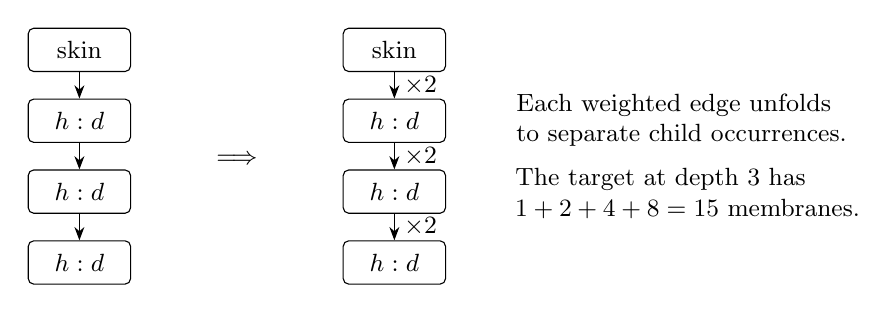
\begin{tikzpicture}[>=Stealth,every node/.style={font=\small},box/.style={draw,rounded corners=2pt,minimum width=1.3cm,minimum height=.55cm}]
\node[box] (s) at (0,2.7) {skin};
\node[box] (a) at (0,1.8) {$h:d$};
\node[box] (b) at (0,.9) {$h:d$};
\node[box] (c) at (0,0) {$h:d$};
\draw[->] (s)--(a);\draw[->] (a)--(b);\draw[->] (b)--(c);
\node at (2,1.3) {$\Longrightarrow$};
\node[box] (t) at (4,2.7) {skin};
\node[box] (x) at (4,1.8) {$h:d$};
\node[box] (y) at (4,.9) {$h:d$};
\node[box] (z) at (4,0) {$h:d$};
\draw[->] (t)--node[right] {$\times2$}(x);
\draw[->] (x)--node[right] {$\times2$}(y);
\draw[->] (y)--node[right] {$\times2$}(z);
\node[align=left,text width=4.3cm] at (7.7,1.35) {Each weighted edge unfolds to separate child occurrences.\\[5pt]The target at depth 3 has\\$1+2+4+8=15$ membranes.};
\end{tikzpicture}
\caption{A source chain and the shared target DAG for simultaneous weak division. Arrows describe parent-to-child containment in this figure.}
\label{qoc:mm:fig:nested}
\end{figure}

\Needspace{9\baselineskip}
\begin{proposition}[Exact nested-family ledger]
For this family the generic dense certificate has
\[
 K=2D+1,\quad J=D+1,\quad A=2D,\quad E=D,\quad L=2D+1,
\]
with $d=1$ and $B=Z=0$. Therefore
\[
 V=2D^2+11D+5,\qquad R=8D^2+15D+7.
\]
\end{proposition}
\begin{proof}
There are $D+1$ source shapes including skin and $D+1$ target shapes including skin. Their elementary leaf shape is shared, while the other shapes differ in child multiplicity or skin population, giving $2D+1$ configuration entries and $2D$ supported configuration edges. There is one decorated transition per old depth, including skin, giving $D+1$ transitions and $D$ transition edges. Each inner division has two target references and the skin has one. No evolution exists, and every potentially dividing inner membrane has its slot occupied, so no maximality equation is needed. Substitution in Theorem~\ref{qoc:mm:thm:ledger} gives the formulas.
\end{proof}
At $D=10$, the target has 2047 membranes, while the compiler uses 315 coordinates and 957 residuals. The degree bound stays unchanged. Quadratic growth here reflects the dense $KJ$ forest coordinates, not an assertion that this representation is minimal.

\subsection{A sharp one step bound on expanded membrane population}
The nested family also attains the largest possible next population for a fixed old population in this model. This follows directly from the same copying convention and does not claim a new literature result.

\begin{proposition}[Exact population identity and sharp bound]
Let an old tree contain $n$ membranes including the fixed skin. For each old membrane $v$, let $a(v)$ count the selected dividing membranes on the path from skin to $v$, including $v$ itself when it divides. If $\mathcal D$ is the set of old membranes selected for dissolution, the number of membranes after the step is exactly
\[
 N_{\rm next}=\sum_{v\notin\mathcal D}2^{a(v)}\leq 2^n-1.
\]
A chain of $n-1$ inner membranes all selecting weak division attains equality.
\end{proposition}
\begin{proof}
Temporarily tag each old membrane by its old tree occurrence; these tags are only for this counting proof. A surviving old membrane contributes one updated root before copying by enclosing divisions. Each selected division on its ancestor path doubles that contribution. If the membrane itself divides, its own root contribution doubles as well. Dissolution removes its own root but passes all already updated descendants onward without multiplying or deleting their roots. Consequently each nondissolving old membrane contributes exactly $2^{a(v)}$ roots to the final tree, and each dissolving one contributes none. Distinct old tags give disjoint root contributions, proving the identity.

Index all old vertices as $v_0,\ldots,v_{n-1}$ in nondecreasing depth, with the skin $v_0$ at depth zero. Every strict ancestor occurs earlier, so $\operatorname{depth}(v_j)\leq j$. The skin cannot divide, hence $a(v_j)\leq\operatorname{depth}(v_j)$. Adding back the omitted nonnegative terms for dissolved vertices gives
\[
 N_{\rm next}\leq\sum_{j=0}^{n-1}2^{\operatorname{depth}(v_j)}
 \leq\sum_{j=0}^{n-1}2^j=2^n-1.
\]
For a chain with every inner membrane dividing, no root is dissolved and $a(v_j)=j$ for every vertex. Both inequalities become equalities.
\end{proof}
Thus even one simultaneous weak-division step can expand exponentially in the old physical population. The motif description remains polynomial for the maximally expanding chain because its many new subtrees coincide.

\subsection{Contextual dissolution followed by copying}\label{qoc:mm:sec:contextcopy}
Let the alphabet be $\{a,b,c\}$, and use rules
\[
 [a]_p\to[a]_p[a]_p,\qquad [b]_q\to c.
\]
The skin has two $p$-children, each containing one $a$. Only the first has a $q$-child, carrying $b$. Both $p$-membranes divide, and the $q$-membrane dissolves. Its updated output $c$ first enters its own parent's $Y$ vector. Division copies that vector into both daughters. The target is exactly two $p$-membranes with payload $ac$ and two with payload $a$; none retains a $q$-child.

In arithmetic, $O_q=\ee_c$ and $F_q=0$. The first parent's $G$ is zero and $Y=\ee_c$ after its $a$ is reserved for division; the second parent's $Y=0$. The daughter equations then add $\ee_a$ to the correct pair. Sharing the generic division rule does not share the two parents' updated payloads. The package exports all 129 residuals and the 86-coordinate witness for this example as explicit sparse integer polynomials.

A more deeply nested regression lets two successive dissolutions promote an emptied leaf and all released objects, then lets an ancestor divide into differently marked daughters. The expected target is written down independently of the polynomial evaluator. This checks forest promotion as well as object copying.

\section{Necessary distinctions and a worst case obstruction}\label{qoc:mm:sec:limits}
\subsection{Aggregate mass cannot determine a transition}
Consider two configurations with two elementary $h$-membranes and a total of two copies of $a$. In the first, the payloads are $(aa,\varnothing)$; in the second, they are $(a,a)$. With the sole rule $[a]_h\to[b]_h[b]_h$, the first configuration has one applicable structural slot and produces three $h$-membranes. The second has two and produces four. Both selections are forced and maximal. Equal global object mass and membrane population therefore fail to specify an exact next state.

\subsection{Source-identical children can split their choices}
Let a skin hold one $a$ and two empty elementary $h$-children. The only rule is $a[\ ]_h\to[b]_h$. Sending into neither child is not maximal; sending into both overspends the skin's old $a$. Exactly one child must receive. A representation insisting that all source-identical children take the same mode would reject every legal schedule.

The transition catalogue solves this by using two decorated child types with the same source reference: one idle and one receiving. Their positive populations add to the source multiplicity in~\eqref{qoc:mm:eq:S}. For this example each population is one. The split is genuine computation-level nondeterminism, not a nonunique value of a derived auxiliary.

\subsection{Separate parents keep separate budgets}
Give each of two $p$-parents one empty $h$-child, and put one $a$ only in the first parent. Under the same send-in rule, the first child must receive and the second cannot. Swapping these two choices preserves every global population total, but uses an unavailable old object in the second parent and leaves an addable rule in the first. Resource and maximality equations are therefore both naturally local to a parent transition motif.

\subsection{New objects wait until the next step}
Let a skin have no old objects and contain a $q$-child with one $a$ and an empty $h$-child. With $[a]_q\to b$ and $b[\ ]_h\to[a]_h$, the $q$-child dissolves. The $h$-child must remain idle this step because the parent had no old $b$. The new $b$ appears in the target skin and can be used only in a later step. Replacing~\eqref{qoc:mm:eq:R} by a balance that already included upward outputs would accept the wrong transition.

The same distinction applies to elementary restrictions. A membrane with children in the old configuration cannot select an elementary-only division merely because those children dissolve later in that step. Rule availability is checked on the old topology.

\subsection{A fixed deterministic system with exponentially many distinct motifs}
Use one inner label $h$, alphabet $\{a,d,u,v\}$, and exactly four rules:
\begin{align*}
 [a\to aa]_h,\qquad [u\to d]_h,\qquad [v\to da]_h,\qquad
 [d]_h\to[u]_h[v]_h.
\end{align*}
Start with an empty skin and one elementary $h$-membrane containing $d$. A round consists of a division step and a recovery step.

\begin{theorem}[Exponential obstruction to identical-subtree sharing]\label{qoc:mm:thm:antishare}
After $2T$ steps, this fixed system has exactly $2^T$ elementary $h$-membranes, with pairwise distinct payloads
\[
 d\,a^{n(\varepsilon)},\qquad
 n(\varepsilon)=\sum_{i=0}^{T-1}\varepsilon_i4^i,
 \qquad\varepsilon_i\in\{0,1\}.
\]
The configuration is deterministic up to permutation of indistinguishable occurrences. Every exact representation that merges only identical rooted configuration subtrees needs at least $2^T$ distinct leaf motifs at that time.
\end{theorem}
\begin{proof}
At a round boundary, suppose a leaf contains $da^n$. Its only structural trigger is $d$, so maximality forces division. Every old $a$ must evolve to $aa$, giving $2n$ copies before the updated local multiset is copied. The two daughters therefore have $ua^{2n}$ and $va^{2n}$.

In the recovery step no division is possible because no old $d$ exists. Every $a$ doubles again. The unique $u$ evolves to $d$ and the unique $v$ evolves to $da$. The resulting boundary payloads are thus $da^{4n}$ and $da^{4n+1}$. No alternative rule competes for any symbol in either phase, and no communication exists, so the selected applications are forced modulo permutations.

The initial exponent is zero. Repeatedly applying the two maps $n\mapsto4n$ and $n\mapsto4n+1$ gives exactly the stated base-4 digit set after $T$ rounds. Distinct binary digit strings give distinct base-4 integers: at the greatest differing position $r$, the discrepancy $4^r$ exceeds the sum $1+4+\cdots+4^{r-1}=(4^r-1)/3$ of all possible lower discrepancies. There are consequently $2^T$ distinct payload vectors and $2^T$ leaves. An exact identical-subtree quotient cannot merge any two of those leaves, proving the lower bound.
\end{proof}
The lower bound applies only to equality-based subtree quotients. It is not a lower bound on all arithmetic encodings, symbolic set descriptions, generating functions, or circuit representations. Indeed, the displayed base-4 digit condition is itself a concise symbolic description. The replay checks eight rounds, yielding 256 distinct leaf payloads; the unbounded claim rests on the proof.

\section{Finite traces and the universality boundary}\label{qoc:mm:sec:universality}
\subsection{Composing steps is possible but costs interfaces}
For any prescribed finite number of steps, choose a certificate for each step and join its target to the next source using a consistently shared configuration representation or explicit interface constraints. Accumulate the skin output vectors with linear equations. These added coordinates and equations must be included in a trace-level ledger; they are absent from~\eqref{qoc:mm:eq:V} and~\eqref{qoc:mm:eq:Rcount}.

A terminal idle step, with every structural mode idle and every evolution count zero, tests that no rule is enabled. Its maximality conditions force all otherwise usable old triggers to be absent. Thus a finite halting trace can be certified without requiring a first-halting-time convention or a canonical accepting trace. On the other hand, the number of slices remains a parameter. Nothing here collapses an unbounded computation history to a fixed number of coordinates.

\subsection{A suitable universal-model compiler candidate}
Alhazov, Freund, and Riscos-N\'u\~nez~\cite{mm:alhazov}, Theorem 4.1, give an effective two-register-machine compiler using noncooperative symbol objects, one polarization, fixed labels, elementary division, and dissolution. Its four initial membranes include two counter-labelled membranes and an inner control membrane. At simulation boundaries, register $i$ is represented by the number of empty $i$-membranes minus one; the spare membrane permits future increment by division. Output is interpreted only along halting computations. This is a particularly relevant frontend because its unbounded numerical state resides in membrane populations.

That source result is an effective compiler parameterized by a finite register program. It does not, by itself, print a particular universal finite interpreter together with a proved external-input encoding. Its generative convention starts with zero registers. A separately specified input loader and program instantiation are required before claiming the requested literal universal object.

There are also explicit transcription obligations. The printed output-rule display includes a continuation not bound by its stated one-successor output instruction; an executable version must remove the extraneous alternative or change the source instruction contract. Adjacent support rules require their intended separation. These repairs must be declared, not silently incorporated into a purported verbatim source rule table.

The source labels both the skin and an inner control membrane by $s$, whereas our schema uses a unique skin label. A compatible role split renames only the outer membrane to $\sk$, retains the inner $s$-rules, and duplicates the source $s$-labelled evolution and send-out rules for the skin. It adds no skin send-in. The translation adds one label, so the source's original three-label count cannot be carried over unchanged. This article does not ship a certified instantiated universal rule table.

\begin{writenote}
Part~\ref{qoc:um:part} (source~16, delivered with this source) carries out exactly these obligations for the compiler of Alhazov, Freund and Riscos-N\'u\~nez: it separates the two support rules, uses no output instruction (so the extraneous output alternative plays no role), splits the skin and inner $s$ roles at the cost of one label, proves an arbitrary-input acceptor with existential global halting directly, and instantiates it literally for the Neary--Woods machine (Section~\ref{qoc:um:sec:sources}, Theorem~\ref{qoc:um:thm:main}). Neither source cites the other.
\end{writenote}


\subsection{Other sources and claims deliberately left open}
The original P\u aun--Suzuki--Tanaka--Yokomori division construction supplies another effective compiler through a matrix grammar~\cite{mm:paun}. The available original preprint and the final published article are distinct provenance objects; byte-for-byte identity has not been established. Its relevant elementary division construction uses charge states, so it is not directly the polarizationless implementation proved here. A no-polarization result with label-changing division belongs to another variant. Freund and P\u aun's no-polarization construction~\cite{mm:freund} uses string objects; it must not be treated as the present symbol-object model.

These sources support model-level computational completeness in carefully delimited variants. They do not close the remaining chain of obligations: a literal finite universal source program, an external-input convention and loader, an exact frontend simulation proof after any repairs, an unbounded-time arithmetic decoder, and a fully charged fixed-arity equation ledger. The quartic sum of squares here is schema-dependent. No improvement on a smallest known fixed universal Diophantine polynomial, no tiny universal operation count, and no world-first compression claim follows.

\begin{writenote}
Of the chain of obligations listed in the last paragraph, Part~\ref{qoc:um:part} supplies the literal finite universal source program, an external-input convention with an affine structural loader (the bridge from an ordinary input to half tapes stays external), and the exact frontend simulation proof. An unbounded-time arithmetic decoder and a charged fixed-arity equation ledger remain open there as well.
\end{writenote}


\section{Replay design and evidence limits}\label{qoc:mm:sec:replay}
\subsection{What is executable}
The release contains a standard-library-only Python implementation of exact sparse integer polynomial arithmetic. It builds named scalar residuals from a supplied schema and evaluates them with arbitrary-precision integers. It also contains an expanded operational oracle: it first allocates old objects at concrete membrane occurrences, checks slots and addability of rules, and then performs bottom-up structural execution.

The two routes serve different purposes. The oracle exposes old-object use and physical tree construction directly. The compressed evaluator checks the derived equations without expanding populations. The tests compare them on bounded examples, but they share some data structures and helper functions. Passing tests are executable corroboration, not a machine-checked proof or a completely independent second implementation.

The exhaustive small suite examines 48,621 candidate plans, of which 2,123 are legal, and checks 160,332 residuals on the legal cases. It includes invalid resource allocations and nonmaximal schedules. Additional regressions exercise separate parents, mixed modes among source-identical children, same-step output exclusion, contextual dissolution and copying, nested division through depth 10, and arbitrary-size integer populations. It rejects 275 single-coordinate mutations of derived auxiliaries in the selected nested example. These are finite coverage counts, not estimates of all possible schemas.

\subsection{Polynomial export format}
In \file{contextual_copy_polynomials.json}, each residual is a list of pairs
\[
 [\text{integer coefficient},\ \text{sorted list of variable names}].
\]
The empty list denotes a constant monomial; a list of one or two names denotes the corresponding product, with repeated names permitted. Variables are natural numbers. The polynomial conjunction is exactly the vanishing of the sum of the squares of the named residuals. No floating-point approximation is used.

The companion \file{contextual_copy_quartic.json} contains the literal expanded sum of squares for this example: degree 4, 282 monomials, and coefficient height 19. Its valid witness evaluates to zero; the tested unit change to one $U$ coordinate gives value 2. This exported polynomial is one contextual example, not a fixed universal equation.

The prefixes \file{x}, \file{c}, \file{m}, \file{e}, \file{u}, \file{y}, \file{o}, and \file{f} correspond to the coordinates defined above. The \file{c} and \file{m} coordinates are shifted by one; their raw values are not the physical child populations. Rule arrays, labels, mode indices, and catalogue references remain schema data.

\subsection{How to reproduce}
From the release root, run
\begin{lstlisting}
python3 replay/run_all.py
\end{lstlisting}
This runs the finite suites, replays the saved examples, exports the contextual polynomials, and records file hashes and execution metadata. Alternatively, from \file{replay/}, run the scripts individually:
\begin{lstlisting}
python3 replay_tests.py
python3 focused_tests.py
python3 verify_saved_examples.py
python3 regression_extensions.py
python3 export_sos.py
\end{lstlisting}
The exhaustive suite can take several minutes. The saved-example verifier alone is the short replay route. Python 3 with its standard library suffices for the arithmetic package. Building the article additionally needs a LaTeX installation with the packages in its preamble:
\begin{lstlisting}
cd article
latexmk -pdf -interaction=nonstopmode -halt-on-error membrane_motifs.tex
\end{lstlisting}

The release includes the article source and PDF, scripts, generated example data, exact residual export, verification receipts, and source URL/hash provenance. It excludes third-party source PDFs, OCR images, and internal review notes. Source checks and front-end typo repairs remain logically separate obligations from the arithmetic compiler proof.

\begin{writenote}
In this report the six replay scripts \path{replay/*.py} are \path{code/15-membrane-motifs-*.py}; the exports, receipts and saved transcripts of \path{replay/} are \path{data/15-membrane-motifs-*} (for example \file{contextual_copy_polynomials.json} is \path{data/15-membrane-motifs-contextual_copy_polynomials.json}); \path{provenance/source-provenance.json} is \path{data/15-membrane-motifs-source-provenance.json}; and the release notes are \path{15-membrane-motifs-RELEASE_NOTES.md}. The article source and PDF named above are this Part and are not shipped, nor are the delivered README and the two checksum ledgers; the transcripts \path{export_sos_stdout.txt} and \path{focused_tests_stdout.txt} are byte-identical to the shipped quartic and focused receipts and are not shipped separately. The scripts rewrite their receipts in place: run them only on a copy in the delivered layout, with \texttt{py} for \texttt{python3} on this machine (the report's README gives the commands). At the write, \path{focused_tests.py} and \path{verify_saved_examples.py} passed on such a copy, and at placement all four short suites did; the exhaustive \path{replay_tests.py} needs several minutes (the research programme's review ran it within its 300-second limit).
\end{writenote}


\section{Conclusion}\label{qoc:mm:sec:conclusion}
Repeated subtrees can be represented exactly without introducing a separate block of arithmetic variables for every physical membrane. The essential ingredients are decorated schedules, per-parent source projection, old-object budgeting, and bottom-up forest equations. Together they yield quadratic residuals and a quartic sum-of-squares certificate with a completely explicit ledger.

The saving is genuine on infinite symmetric families and conditional on the availability of sharing. The deterministic base-4 construction shows why even a fixed small rule set can destroy all identical-leaf sharing. The result therefore provides a precise spatial compression theorem with an explicit boundary, rather than a general escape from the size of computation histories or a fixed universal-polynomial record.

\clearpage
\part{Literal universal active membrane frontends and quadratic outcome certificates}\label{qoc:um:part}

\begin{writenote}
Part~\ref{qoc:um:part} prints source~16 (batch-79 manuscript~09, archive \path{Universal_Membrane_Research_Package.zip}). Its Section~$n$ is Section~$n+49$ here (Sections~\ref{qoc:um:sec:intro}--\ref{qoc:um:sec:future}), its Theorem~$n.m$ is Theorem~$(n+49).m$, and its appendix A is Appendix~\ref{qoc:um:app:artifacts}. Source~16 names no repository commit. It uses the universal machine of Part~\ref{qoc:part:wf}, the Neary--Woods machine $U_{15,2}$ in the same two-half-tape convention, but by a different route: it compiles the transition table into literal counter programs, where Part~\ref{qoc:part:wf} goes through Iijil's 46-clock Waterfall matrix. No theorem is shared; the two are compared in a note after Table~\ref{qoc:um:tab:quadratic}. Source~16 discharges the universal-frontend obligations that Part~\ref{qoc:mm:part} lists in Section~\ref{qoc:mm:sec:universality}. Its program layer (the 528-row three-counter program, the 8,408-row prime-coded program, the macro lemmas and the branch-gate polynomial) is reused without citation by source~17 in Part~\ref{qoc:rn:part}; it is printed once, here. The research programme reviewed source~16 (\path{review_membrane_reports_2a8a.md}, commit \texttt{85294a527}): no theorem-level defect, no false certificate, no patch; its bounded projection of the affine-frontend polynomial is a dated note after Table~\ref{qoc:um:tab:quadratic}.
\end{writenote}

\begin{center}
{\large\bfseries Literal universal active membrane frontends and quadratic outcome certificates}\\[3pt]
{\small Research manuscript. 2 October 2026.}
\end{center}

\begin{abstract}
We give two fully literal polarizationless noncooperative active-membrane frontends for the displayed Neary--Woods 15-state two-symbol universal Turing machine. An affine two-half-tape loader uses a 528-instruction three-counter program, 2,544 membrane rules, 1,296 symbols and five labels. A complementary prime-encoded frontend uses 8,408 two-counter instructions, 34,605 rules, 19,162 symbols and four labels; every positive raw input $a$ simulates half tapes $(v_2(a),v_3(a))$. Both accept by existence of a globally halting maximally parallel run, with erroneous guesses trapped forever. A direct degree-two outcome polynomial at externally fixed instruction time $T$ uses $2{,}811T$ witnesses and $5T+1$ affine squares for the affine frontend, or $29{,}904T$ witnesses and $4T+1$ squares for the prime frontend. The respective nonnegative-product counts are $761T$ and $10{,}748T$. Fibers are empty or singleton even over nonnegative real witnesses at natural inputs. The prime language has a transcendental density of Turing degree $\mathbf0'$, zero effective Hausdorff and packing dimensions, and an explicit $O(\log^2 N)$ counting remainder for its noncomputable counting function. All tables, generators and check receipts accompany the proofs. Unknown time remains unpaid; no fixed-arity unbounded-time representation, efficiency record or priority claim is asserted.
\end{abstract}
\section{The result and its scope}\label{qoc:um:sec:intro}
We use $\N=\{0,1,2,\ldots\}$. A counter instruction has one of the forms
\[
 \ell:\ADD(i,q),\qquad \ell:\SUB(i,q,z).
\]
The first increments counter $i$ and proceeds to $q$. The second decrements a positive counter and proceeds to $q$, or leaves a zero counter unchanged and proceeds to $z$. The distinguished control $\HALT$ has no instruction. ``Physical time'' below counts these individual literal counter instructions, not Turing-machine steps or membrane steps.

The only external universality input is the finite-tape simulation theorem for the displayed Neary--Woods machine~\cite{um:NW}. All subsequent translations are explicit here and in the accompanying finite data. In particular, an unspecified universal two-counter program is not an assumption.

\begin{theorem}[Two literal structural-input frontends]\label{qoc:um:thm:main}
There are fixed finite active-membrane rule sets with the following properties.
\begin{enumerate}
\item The affine frontend has 2,544 rules, 1,296 object symbols and five labels $\{\skin,1,2,3,s\}$. For any $L,R\in\N$, its skin contains the fixed entry object, $L+1$ empty label-$1$ children, $R+1$ empty label-$2$ children, one empty label-$3$ child and one empty delay $s$. It has a globally halting maximally parallel computation exactly when the machine in Table~\ref{qoc:um:tab:tm} halts from state $\mathrm A$, scanned bit $0$, and half tapes $(L,R)$.
\item The prime frontend has 34,605 rules, 19,162 object symbols and four labels $\{\skin,1,2,s\}$. For each $a\geq1$, its skin contains the fixed entry object, $a+1$ empty label-$1$ children, one empty label-$2$ child and one empty delay. It has a globally halting maximally parallel computation exactly when that same source machine halts on $(v_2(a),v_3(a))$.
\end{enumerate}
Both structural-input halting languages are computably enumerable complete. Their initial populations are respectively $L+R+5$ and $a+4$, including the skin.
\end{theorem}

The rule set, alphabet, labels and initial control are fixed. The expanded initial membrane tree is \emph{not} fixed. The first frontend has affine loading in its two half-tape inputs; the second trades one membrane label for a single positive-integer interface. Valuations specify the mathematical input contract; there is no valuation or factorization primitive among the rules. The exact simulation uses only literal increment/decrement instructions and membrane operations.

Acceptance means \emph{existence of a globally halting run}: no rule is enabled anywhere in its last configuration. It does not mean merely that $\HALT$ is present. Nor does it mean that all branches halt. The counter program is deterministic, but wrong membrane allocations can enter a persistent trap even when an accepting branch exists.

The output is an explicit frontend for further arithmetization. Section~\ref{qoc:um:sec:quadratic} already supplies a direct bounded-time quadratic outcome polynomial. Unknown time, however, is not compressed into a fixed finite witness tuple. The construction makes no claim to a new small universal-machine bound, a new singlefold MRDP representation, a small-operation Diophantine record, or literature priority.

\begin{table}[ht]
\centering
\begin{tabular}{lrr}
\toprule
Fixed component & Affine frontend & Prime frontend\\\midrule
Literal counter instructions & 528 & 8,408\\
\quad $\ADD$ instructions & 295 & 6,068\\
\quad $\SUB$ instructions & 233 & 2,340\\
Membrane rules & 2,544 & 34,605\\
Object symbols & 1,296 & 19,162\\
Membrane labels & 5 & 4\\
Initial expanded membranes & $L+R+5$ & $a+4$\\
\bottomrule
\end{tabular}
\caption{Two fixed-rule frontends for the same 29-row source Turing machine. Initial population is an input cost, not a fixed constant.}\label{qoc:um:tab:ledger}
\end{table}

\section{Sources and the exact machine}\label{qoc:um:sec:sources}
\subsection{Primary sources and source corrections}
Neary and Woods give the 15-state two-symbol universal Turing machine in Table~16 of~\cite{um:NW}, together with its effective finite bi-tag encoding. We rename states $u_1,\ldots,u_{15}$ as $\mathrm A,\ldots,\mathrm O$ and symbols $c,b$ as $0,1$. The primary table has $u_{15},b\mapsto b,R,u_{14}$ and leaves $u_{10},b$ undefined. Thus $\mathrm{J}1$ is the unique undefined instruction. A conflicting later prose reference to $u_{10},c$ is not used. The universal initial head scans the rightmost $c$ in the encoded marker $G=bc$, in state $u_1$; both half tapes may vary. The finite serialized table~\cite{um:serialization} is included with a pinned SHA-256 digest and is checked against these conventions.

\begin{writenote}
The inconsistency described here (the undefined $(u_{10},b)$ in Table~16 against later prose naming $u_{10},c$) is the one that Part~\ref{qoc:part:wf} reports and resolves in the same way, after Table~\ref{qoc:wf:tab:tm}; the research programme's note \path{neary_woods_explicit_universal_tm.md} recorded it first, and source~17 reports it again (Section~\ref{qoc:rn:sec:source}). The erratum is printed in full only there. Table~\ref{qoc:um:tab:tm} below agrees with Table~\ref{qoc:wf:tab:tm} entry by entry. The serialized table~\cite{um:serialization} is the same file (SHA-256 \texttt{ba70ab2c\ldots}) that Part~\ref{qoc:part:wf} uses; it is third-party data, not covered by the repository's MIT-0 licence, and is shipped once, as \path{data/14-waterfall-UniversalTM15x2.tm.txt}. Source~16's two copies of it are not shipped.
\end{writenote}


The membrane compiler is adapted from Theorem~4.1 of Alhazov, Freund and Riscos-N\'u\~nez~\cite{um:AFR}. That source concerns nondeterministic two-register \emph{generation from zero registers}. An arbitrary-input recognizer does not follow from its statement alone. Sections~\ref{qoc:um:sec:rules}--\ref{qoc:um:sec:memproof} prove the structural-input and existential-global-halting adaptation directly.

For clarity, we retain the following display corrections and choices:
\begin{enumerate}
\item The displayed $[t\to\eps]_s$ and $[d\to\trap]_s$ are two separate rules.
\item A counter value is its associated membrane population \emph{minus one}; the spare empty membrane is needed for later division.
\item Deterministic $\ADD$ takes the same continuation in both source alternatives. Identical duplicate outgoing rules are stored once.
\item No output instruction is used. The source display's extraneous unbound double-prime output alternative plays no role.
\item Program labels, instruction-specific auxiliary symbols, and the support objects $b_i,d,t,\trap$ are pairwise disjoint.
\item The source uses label $s$ for both skin and inner delay. We rename the outer label $\skin$, keep inward $s$ rules aimed at the delay, and put every source $s$-labelled evolution and send-out rule at \emph{both} labels. This conservative split gives four labels for the prime frontend and five for the affine frontend; the source's original three-label count is not claimed.
\item Unused source output-alphabet decorations are omitted. The exported alphabet is exactly the union of symbols actually appearing in rules.
\end{enumerate}
These choices introduce no polarization, priorities, cooperative rules, changing labels, membrane creation, or non-elementary division.

\subsection{The full source transition table}
At a Turing cut the currently scanned symbol is in finite control. The integer $L$ records the successive symbols strictly to the left, least significant bit nearest the head; $R$ records the analogous right half. High omitted bits are blank $0$. Thus every pair of natural numbers specifies a finite nonblank tape with scanned bit $0$ at the initial cut.

\begin{table}[ht]
\centering
\begin{tabular}{ccc@{\qquad}ccc}
\toprule
State & Read $0$ & Read $1$ & State & Read $0$ & Read $1$\\\midrule
$\mathrm A$ & $(0,R,\mathrm B)$ & $(1,R,\mathrm A)$ & $\mathrm I$ & $(0,R,\mathrm A)$ & $(1,L,\mathrm J)$\\
$\mathrm B$ & $(1,R,\mathrm C)$ & $(1,R,\mathrm A)$ & $\mathrm J$ & $(1,L,\mathrm K)$ & undefined\\
$\mathrm C$ & $(0,L,\mathrm G)$ & $(0,L,\mathrm E)$ & $\mathrm K$ & $(0,R,\mathrm L)$ & $(1,R,\mathrm N)$\\
$\mathrm D$ & $(0,L,\mathrm F)$ & $(1,L,\mathrm E)$ & $\mathrm L$ & $(0,R,\mathrm M)$ & $(1,R,\mathrm L)$\\
$\mathrm E$ & $(1,R,\mathrm A)$ & $(1,L,\mathrm D)$ & $\mathrm M$ & $(0,L,\mathrm B)$ & $(1,R,\mathrm L)$\\
$\mathrm F$ & $(1,L,\mathrm D)$ & $(1,L,\mathrm D)$ & $\mathrm N$ & $(0,L,\mathrm C)$ & $(0,R,\mathrm O)$\\
$\mathrm G$ & $(0,L,\mathrm H)$ & $(1,L,\mathrm G)$ & $\mathrm O$ & $(0,R,\mathrm N)$ & $(1,R,\mathrm N)$\\
$\mathrm H$ & $(1,L,\mathrm I)$ & $(1,L,\mathrm G)$ & & &\\\bottomrule
\end{tabular}
\caption{Each defined entry gives written bit, head direction, and next state. This is the exact source table used throughout.}\label{qoc:um:tab:tm}
\end{table}

\section{The three-counter simulation}\label{qoc:um:sec:virtual}
The virtual registers are $L,R,K$, where $K$ is scratch. We use $K$ here to avoid confusing the scratch register with the externally fixed physical time $T$ of Section~\ref{qoc:um:sec:quadratic}; the code names the scratch register \file{T}. At every Turing cut $K=0$. The scanned bit and Turing state are encoded in the program label.

The one-instruction prologue
\[
 \mathsf{init}:\SUB(K,\mathsf{init},\mathsf{entry}_{\mathrm A0})
\]
clears arbitrary initial $K$ and takes $K+1$ virtual instructions. This will make the eventual prime-encoded input contract valid on \emph{every} positive integer.

Fix a defined transition $(q,s)\mapsto(w,D,q')$. Let $X$ be the half tape in direction $D$ and $Y$ the other half. The following labels are fresh for the transition and parity branch. Aliases are resolved by the generator, so the exported program contains no macro instructions or unresolved edges.

\subsection{Pop the next scanned symbol}
The first loop is
\begin{align*}
 \mathsf{pop}_0&:\SUB(X,\mathsf{pop}_1,\mathsf{back}_0),\\
 \mathsf{pop}_1&:\SUB(X,\mathsf{pair},\mathsf{back}_1),\\
 \mathsf{pair}&:\ADD(K,\mathsf{pop}_0).
\end{align*}
Write the initial value $X_0=2Q+r$ with $r\in\{0,1\}$. After $k$ complete loops,
\[
 X=2(Q-k)+r,\qquad K=k,\qquad 0\leq k\leq Q.
\]
When $k<Q$ both decrements succeed. At $k=Q$ the first test fails if $r=0$, while one decrement succeeds and the second test fails if $r=1$. The rank $Q-k$ decreases on complete loops, so exit is inevitable. The exit has $X=0,K=Q$, with $r$ in finite control.

Each parity-specific recovery loop is
\[
 \mathsf{back}:\SUB(K,\mathsf{backadd},\mathsf{push}),\qquad
 \mathsf{backadd}:\ADD(X,\mathsf{back}).
\]
After $j$ successful transfers $X=j,K=Q-j$. Decreasing $K$ proves termination with $X=Q,K=0$. The pop and recovery together execute
\[
 3Q+(1+r)+(2Q+1)=5Q+r+2
\]
virtual instructions.

\subsection{Push the written symbol}
The other half is doubled and restored by
\begin{align*}
 \mathsf{push}&:\SUB(Y,\mathsf{twice}_1,\mathsf{restore}),\\
 \mathsf{twice}_1&:\ADD(K,\mathsf{twice}_2),\\
 \mathsf{twice}_2&:\ADD(K,\mathsf{push}),\\
 \mathsf{restore}&:\SUB(K,\mathsf{restoreadd},\mathsf{write}),\\
 \mathsf{restoreadd}&:\ADD(Y,\mathsf{restore}).
\end{align*}
Starting from $Y=Y_0,K=0$, after $k$ first-loop iterations,
$Y=Y_0-k,K=2k$. The rank $Y_0-k$ decreases to zero. The recovery loop preserves $Y+K=2Y_0$ and decreases $K$, ending at $Y=2Y_0,K=0$. If $w=1$, one $\ADD(Y,\mathsf{entry}_{q'r})$ follows. If $w=0$, the write label is an alias for that next entry. This stage costs $7Y_0+2+w$ instructions.

\begin{lemma}[Exact virtual simulation]\label{qoc:um:lem:virtual}
Every defined Turing transition, on all natural half tapes, maps
\[
 (X,Y,K)=(2Q+r,Y_0,0)\longmapsto(Q,2Y_0+w,0)
\]
and sets control to $(q',r)$. It executes exactly
\[
 C_{\mathrm v}=5Q+r+7Y_0+w+4
\]
virtual instructions. All internal loops terminate and none can halt prematurely.
\end{lemma}
\begin{proof}
The invariants and decreasing ranks just proved give every step and its exact count. Removing the least significant bit of $X$ makes that bit the new scan; doubling $Y$ and adding $w$ pushes the written symbol onto the opposite half. These are precisely the two-half-tape semantics of moving the head in direction $D$. The only halt edge is the undefined source state $\mathrm J1$. Induction over finite prefixes yields the asserted simulation, and an infinite source computation yields infinitely many terminating virtual macros.
\end{proof}

A cut is not determined by a control label alone. The pop loop revisits its first label with positive scratch. A genuine Turing cut requires both the designated entry label and $K=0$. The supplied direct replay uses that condition.

Across the 29 source rows and the prologue, the program has 528 literal instructions. Its per-register counts are
\[
\begin{array}{c|rrr}
 &L&R&K\\\hline
\ADD&74&76&145\\
\SUB&58&58&117
\end{array}
\]
and these numbers are verified from the saved table.

\section{The affine three-counter frontend}\label{qoc:um:sec:direct}
The 528-row program is already literal: nothing requires the intermediate prime encoding to use it as a membrane frontend. Apply the membrane construction of Section~\ref{qoc:um:sec:rules} directly to its three counters, using counter labels $1,2,3$ and the two labels $s,\skin$. The proof of Section~\ref{qoc:um:sec:memproof} operates on one selected counter and leaves the others untouched, so it applies to every fixed number of counters.

The loaded counters are $(L,R,0)$. Their spare-membrane populations are $L+1,R+1,1$, together with one delay and the skin, for a total of $L+R+5$. This is an affine loader on the two half-tape integers and performs no prime exponentiation. Expanding the tree still costs its population.

For $d$ counters, the support-rule count is $7d+7$: seven rules per counter, one inward delay rule, and three evolution rules at each of $s,\skin$. The support alphabet has $d+3$ symbols $b_1,\ldots,b_d,d,t,\trap$, where the italic object $d$ is distinct from the numerical counter-count parameter. With 295 additions and 233 subtractions this gives
\begin{align*}
 \#\mathcal R_3&=3(295)+7(233)+28=2{,}544,\\
 \#\Sigma_3&=528+1+295+2(233)+6=1{,}296.
\end{align*}
The only extra change from the two-counter rule schema is the third counter label and its support symbols/rules. No new membrane operation is introduced.

For $(L,R)=(6,0)$, the exact source trace of Section~\ref{qoc:um:sec:example} uses 328 literal three-counter instructions, including 29 failed subtractions. The sole incoming edge into $\HALT$ anywhere in the direct program is \file{tm_I1_1_write}: $\ADD(R,\HALT)$. Thus every direct halting computation has a clean membrane exit. Its correct membrane computation therefore takes
\[
 3(328)+29=1{,}013
\]
steps. Its maximum expanded population is 30. In contrast, the prime frontend uses the enormous exact time computed in Section~\ref{qoc:um:sec:example}. The direct version uses fewer rules and less time here, at the cost of an extra label and a two-input interface. The prime version supplies a distinct one-positive-integer acceptance language and its density theorem; the comparison does not hold the input interface fixed.

\section{Prime encoding into two counters}\label{qoc:um:sec:prime}
\subsection{The all-positive-input representation}
Write the physical counters as $A,B$. At a virtual-instruction boundary,
\begin{equation}\label{qoc:um:eq:prime}
 B=0,\qquad A=c\,2^L3^R5^K,\qquad c\geq1,\quad\gcd(c,30)=1.
\end{equation}
Every positive $A$ has exactly this form, by unique prime factorization. The factor $c$ is preserved. The associated primes are $p_L=2,p_R=3,p_K=5$. During a physical macro $A$ may be zero; only the macro-boundary value must be positive.

The prologue repeatedly performs virtual $\SUB(K)$, hence removes all factors of $5$. It terminates at $A=c2^L3^R,B=0$. It therefore starts the Turing simulation on exactly $(v_2(a),v_3(a))$ for raw input $a$, regardless of $v_5(a)$ or other prime factors. The loader and the program do not factor $a$.

\subsection{Increment by multiplication with a fixed prime}
For a virtual $\ADD$ with prime $p$, drain $A$ one unit at a time, placing $p$ units in $B$ by $p$ consecutive literal $\ADD B$ instructions per successful decrement. Starting with $(A,B)=(N,0)$, after $k$ iterations
\[
 A=N-k,\qquad B=pk.
\]
The nonnegative rank $N-k$ decreases. After the failed drain test, $A=0,B=pN$. A second loop performs $\SUB B$ followed by $\ADD A$ until $B=0$. It preserves $A+B=pN$, decreases $B$, and takes the virtual continuation at $(pN,0)$.

The first loop contains $N$ successful decrements, $pN$ additions, and one failed decrement. The transfer contains $pN$ successful decrements, $pN$ additions, and one failed decrement. Thus
\begin{equation}\label{qoc:um:eq:addcost}
 \#\ADD=2pN,\quad \#\SUB_+=(p+1)N,\quad
 \#\SUB_0=2,\quad C=(3p+1)N+2.
\end{equation}
Multiplication by $p$ increments precisely its represented exponent.

\subsection{Decrement by division with remainder}
For virtual $\SUB$ with prime $p$, use $p$ finite remainder labels $\mathsf{rem}_0,\ldots,\mathsf{rem}_{p-1}$. Each successful test decrements $A$ and advances the remainder label; wrapping around from $p-1$ to $0$ additionally increments $B$. At remainder label $j$ after $k$ complete groups,
\[
 A=N-pk-j,\quad B=k,\quad 0\leq j<p.
\]
The first failed decrement occurs in the unique remainder state $r$ at $A=0,B=Q$, where $N=pQ+r$ and $0\leq r<p$. Every success consumes an $A$ unit; a group addition cannot cycle alone. Hence this phase terminates.

If $r=0$, transfer $B$ to $A$ one-for-one. The invariant $A+B=Q$ and decreasing $B$ give $(A,B)=(Q,0)$. Because $N\geq1$ and $p\mid N$, $Q\geq1$. The positive continuation is correct: divisibility means the represented exponent was positive, and division reduces it by one.

If $r>0$, each successful decrement of $B$ is followed by $p$ consecutive additions to $A$. After $k$ groups $A=pk,B=Q-k$. At $B=0$, execute $r$ final additions to $A$ and take the virtual zero continuation. This restores $(A,B)=(N,0)$ exactly. Nondivisibility by $p$ is precisely exponent zero.

\begin{table}[ht]
\centering
\begin{tabular}{lrrrr}
\toprule
Virtual case & $\ADD$ & $\SUB_+$ & $\SUB_0$ & Total\\\midrule
$\ADD$ at prime $p$ & $2pN$ & $(p+1)N$ & $2$ & $(3p+1)N+2$\\
$\SUB$, $r=0$ & $2Q$ & $N+Q$ & $2$ & $N+3Q+2$\\
$\SUB$, $r>0$ & $N+Q$ & $N+Q$ & $2$ & $2N+2Q+2$\\\bottomrule
\end{tabular}
\caption{Exact physical instruction costs on input $N\geq1$, with $N=pQ+r$. Failed tests count as executed instructions.}\label{qoc:um:tab:cost}
\end{table}

There is no nondeterministic division oracle: a remainder is a bounded control state. Every exit restores $B=0$ and positive $A$ before taking any source continuation, including $\HALT$.

\begin{lemma}[Exact all-input prime simulation]\label{qoc:um:lem:prime}
Each physical macro terminates on every $N\geq1$ satisfying~\eqref{qoc:um:eq:prime}, implements its stated virtual instruction, preserves $c$ and the other exponents, and has the exact counts of Table~\ref{qoc:um:tab:cost}. Consequently the literal two-counter program has the same halting outcome as the source machine for every raw input $a\geq1$.
\end{lemma}
\begin{proof}
The drain, transfer and restoration invariants establish each output and exclude internal nontermination. Unique factorization interprets multiplication and divisibility as exponent increment and guarded decrement. The scratch-clearing prologue is finite, so Lemma~\ref{qoc:um:lem:virtual} applies. Induction over virtual instructions proves finite-prefix correspondence. Since each physical macro is finite, an infinite virtual computation cannot terminate inside a macro or at an unrelated edge.
\end{proof}

An increment macro uses $p+3$ literal rows. A decrement macro uses
\[
 \frac{3p^2+p+4}{2}
\]
rows: respectively $9,17,42$ for $p=2,3,5$. The virtual counts therefore give
\begin{align*}
 &(74\cdot5+76\cdot6+145\cdot8)\\
 &\qquad +(58\cdot9+58\cdot17+117\cdot42)=8{,}408.
\end{align*}
The resulting 6,068 additions and 2,340 subtractions are fully expanded in the export. A physical macro cut, like a Turing cut, requires the mapped entry \emph{and} $B=0$; its internal drain or grouping cycle may revisit that entry while $B>0$.

\subsection{Why finite code checking supports an unbounded proof}
The independent checker reads saved tables rather than importing the generator. It symbolically executes affine straight-line paths, for example
\[
 (A,B)=(x+p,y)\longmapsto(x,y+1),\qquad x,y\in\N,
\]
and corresponding loop exits and restoration tails. At each test, a zero branch has identically zero input; a positive branch has nonnegative affine coefficients and constant at least one. Hence the path is legal for all natural parameter values and its affine output is exact. These checks cover every one of the 528 virtual and 8,408 physical rows.

The arbitrary-length loops are justified by the invariants and well-founded ranks above, not by extrapolating a finite grid. Concrete tests of all six operation/prime shapes, source tape cases and arbitrary cofactors provide additional regression coverage. Neither the scripts nor this manuscript constitute a proof-assistant formalization.

\section{The literal membrane rules}\label{qoc:um:sec:rules}
\subsection{Operational semantics}
Every rule is noncooperative: it consumes one old object. The operations are object evolution, send-in, send-out, dissolution, and elementary division, without polarization. Objects produced during a step become available only in the next step. A membrane may have at most one structural action in a step; evolution on its other old objects can coexist with that action. For send-in, the occupied structural slot is the receiving child boundary. Taking an object from the parent does not occupy the parent's own boundary, so different children can receive distinct old skin objects simultaneously.

Allocations are inclusion-maximal among compatible rule occurrences. The skin is never divided or dissolved. All its children are elementary throughout the construction. Division copies all other current contents to both daughters; dissolution releases them to the parent. These conventions are material to the proof, particularly the simultaneous reservation of different child membranes.

For a fixed counter count $d$, counter $i\in\{1,\ldots,d\}$ with value $n_i$ is represented by $n_i+1$ empty membranes labelled $i$. For each instruction label $\ell$, let $u_\ell$ and, for $\SUB$, $v_\ell$ be fresh objects. They are serialized as the label followed by \file{$1} and \file{$2}, respectively. Let $q$ denote the increment/positive continuation and $z$ the zero continuation.

\subsection{Instruction rules and support rules}
For $\ell:\ADD(i,q)$, the three rules are
\begin{align}\label{qoc:um:eq:addrules}
 \ell[\ ]_i&\longrightarrow[\ell]_i,&
 [\ell]_i&\longrightarrow[u_\ell]_i[t]_i,&
 [u_\ell]_i&\longrightarrow[\ ]_i q.
\end{align}
For $\ell:\SUB(i,q,z)$, the seven rules are
\begin{align}\label{qoc:um:eq:subrules}
 [\ell\to d b_i u_\ell]_{\skin},&\qquad [\ell\to d b_i u_\ell]_s,\\
 u_\ell[\ ]_i&\longrightarrow[u_\ell]_i,\nonumber\\
 [u_\ell]_i&\longrightarrow q\quad\text{(dissolution)},\nonumber\\
 u_\ell[\ ]_s&\longrightarrow[v_\ell]_s,\nonumber\\
 [v_\ell]_s&\longrightarrow[\ ]_s z,\qquad
 [v_\ell]_{\skin}\longrightarrow[\ ]_{\skin}z.\nonumber
\end{align}
The support rules, for $i=1,\ldots,d$ and $h\in\{\skin,s\}$, are
\begin{align*}
 &[t\to\eps]_i,\qquad b_i[\ ]_i\to[b_i]_i,\qquad
 [b_i]_i\to[\ ]_i t,\\
 &[b_i\to\trap]_i,\qquad [b_i\to\trap]_{\skin},\qquad
 [b_i\to\trap]_s,\qquad [\trap\to\trap]_i,\\
 &d[\ ]_s\to[t]_s,\qquad [t\to\eps]_h,\qquad
 [d\to\trap]_h,\qquad [\trap\to\trap]_h.
\end{align*}
There is no rule consuming $\HALT$. The conservative $s/\skin$ duplicates cannot operate on a correctly simulated control object in the wrong region. Trap evolution is present in every label.

For the prime frontend, the complete finite table is \file{membrane_rules.jsonl}; no right-hand side calls an arithmetic function. The number of distinct rules is
\[
 3(6{,}068)+7(2{,}340)+21=34{,}605.
\]
The object alphabet has one symbol per physical instruction, one halt symbol, one auxiliary per addition, two auxiliaries per subtraction, and five support symbols:
\[
 8{,}408+1+6{,}068+2(2{,}340)+5=19{,}162.
\]
By kind, there are 4,696 evolution rules, 10,751 send-in rules, 10,750 send-out rules, 2,340 dissolution rules, and 6,068 division rules.

\section{All membrane branches and global halting}\label{qoc:um:sec:memproof}
\begin{definition}[Soft boundary]
A soft boundary for counter state $(\ell,n_1,\ldots,n_d)$ has $n_i+1$ empty elementary $i$-membranes for $i=1,\ldots,d$, one empty elementary delay membrane $s$, and skin contents $\ell$ with optionally one $t$.
\end{definition}
The optional $t$ matters: a positive subtraction returns its continuation one step before a skin $t$ is erased. At the next instruction's first phase, that old $t$ erases by evolution, which does not occupy a structural slot. It cannot interfere or accumulate.

\begin{lemma}[Persistent trap]\label{qoc:um:lem:trap}
Once $\trap$ occurs, global halting is impossible.
\end{lemma}
\begin{proof}
The only rule consuming a trap object replaces it with itself. Division copies it and dissolution promotes it to the parent; no rule erases or exports it. Thus at least one trap remains in every later configuration, and its evolution is enabled at every membrane label. Even a simultaneous $\HALT$ control does not remove that enabled rule.
\end{proof}

\subsection{Addition}
At a soft boundary at least one $i$-membrane exists. The control has no alternative skin evolution, so maximality forces it to enter one such child. An optional old skin $t$ erases simultaneously. Next the occupied child must divide into a daughter containing $u_\ell$ and a daughter containing $t$. In the third step $u_\ell$ exits as $q$, while the daughter's $t$ erases. All children are empty again and one $i$-membrane was added. This is a clean boundary after exactly three steps. Choosing different identical children changes no represented state.

\subsection{Subtraction and the forced reservations}
In phase one, $\ell$ evolves to $d b_i u_\ell$ in the skin; any old $t$ erases. In phase two, every branch capable of halting must send $d$ into the unique delay child, where it becomes $t$. If this fails, $d\to\trap$ is either chosen or remains an addable evolution required by maximality. Similarly $b_i$ must enter one $i$-child, or its skin trap evolution makes halting impossible. These two send-ins reserve distinct structural slots.

If $n_i>0$, at least one further $i$-child exists. The delay and reserved child are busy, so maximality forces $u_\ell$ into another $i$-child. If $n_i=0$, there is no available $i$-child and the delay is busy, so $u_\ell$ remains in the skin. In particular, sending $u_\ell$ into the delay blocks necessary $d$ entry and forces a trap; reserving the sole $i$-child for $u_\ell$ when $n_i=0$ blocks necessary $b_i$ entry and also forces a trap. The invalid guesses are real branches of the rule system, but none can globally halt.

\subsection{Positive and zero completions}
In phase three $b_i$ must leave its reserved child as $t$ in the skin. Its competing evolution would create a trap. The delay's old $t$ erases.

If $n_i>0$, $u_\ell$ dissolves its distinct $i$-child and becomes $q$ in the skin. The counter population falls by one while preserving its spare. This is the soft boundary $q+t$ after three steps. The $t$ erases in phase four, possibly simultaneously with the first phase of the next instruction. If $q=\HALT$, that cleanup is required before global halting.

If $n_i=0$, the reserved sole $i$-child's send-out still occupies its structural slot. The delay is structurally available because erasing its old $t$ uses evolution only. Maximality therefore forces the waiting $u_\ell$ into the delay as $v_\ell$. In phase four $v_\ell$ exits as $z$ and the skin $t$ erases. The result is a clean zero-counter boundary, after four steps.

\begin{proposition}[Exact existential instruction simulation]\label{qoc:um:prop:mem}
From every soft boundary, a trap-free instruction outcome exists. Every branch that can globally halt has the correct deterministic counter outcome: an addition after three steps, a positive subtraction at a soft boundary after three steps, or a zero subtraction at a clean boundary after four steps. No trap-free internal deadlock is possible.
\end{proposition}
\begin{proof}
The phase analysis lists compatible allocations achieving each stated outcome. Conversely, the trap lemma excludes every allocation violating the necessary reservations or exits. Maximality forces the remaining moves. There are no other live objects or applicable instruction symbols at these configurations; the role-split duplicate rules add no new trap-free choice. The sole residual object is the stated $t$.
\end{proof}

\begin{proof}[Proof of Theorem~\ref{qoc:um:thm:main}]
Each loaded configuration is a clean counter boundary. A globally halting membrane computation contains no trap and hence follows, instruction by instruction, the unique correct counter computation. At a nonhalting boundary a correct start is enabled, and no trap-free internal deadlock exists, so a finite globally halting run must reach the counter halt. Conversely, a finite counter computation has a trap-free membrane realization and, after at most one cleanup step, is globally terminal.

For the affine frontend, Lemma~\ref{qoc:um:lem:virtual} gives the source-machine equivalence immediately from $(L,R,0)$. For the prime frontend, Lemma~\ref{qoc:um:lem:prime} gives the equivalence from $(a,0)$ to the source half tapes $(v_2(a),v_3(a))$. Both languages are c.e. by simulating the deterministic counter programs. Source universality effectively maps an ordinary halting instance to finite half tapes $(L,R)$, directly reducing to the affine language. Composing with the computable map $a=2^L3^R$ reduces to the prime language, since it has precisely those valuations. Both are therefore c.e.-complete.
\end{proof}

\subsection{Exact timing and object usage}
For the particular prime compiler, every virtual-macro exit is either a failed physical $\SUB B$ or the final remainder-tail $\ADD$. Both have clean membrane exits. Thus a generated accepting computation reaches $\HALT$ without pending $t$. If it has $C$ physical instructions, of which $Z$ are failed subtractions, its correct membrane path has exactly
\begin{equation}\label{qoc:um:eq:memtime}
 M=3C+Z
\end{equation}
steps. Every virtual instruction has exactly two failed physical subtractions, so $Z$ is twice the number of executed virtual instructions. Formula~\eqref{qoc:um:eq:memtime} includes overlap of pending-$t$ cleanup with the next instruction; it would need an extra cleanup term for a generic program ending with a positive subtraction.

Every correctly simulated configuration has at most three objects in the entire system. No such bound is claimed for incorrect infinite branches. Membrane population is unbounded and tracks the physical counter values.

\section{The structural loader and its cost}\label{qoc:um:sec:loader}
The raw interface takes a positive integer $a$ and uses only its structural multiplicity: $a+1$ label-$1$ children, one label-$2$ child and one delay. The executable loader emits a sparse descriptor with those three edge multiplicities and a control-bearing skin. This descriptor represents exactly $a+4$ membranes. A compact multiplicity is not a physical population reduction: constructing the expanded tree takes work proportional to its population.

The optional half-tape interface separately computes
\[
 a=2^L3^R.
\]
For example, an elementary implementation performs $L$ doublings and $R$ triplings starting from one. The binary output length is
\[
 \lfloor L+R\log_2 3\rfloor+1.
\]
Although faster exponentiation may be used, this preprocessing is still external, can have output length exponential in the bit lengths of $L,R$, and is not a fixed number of bounded-degree arithmetic operations. It is paid in the completeness reduction.

\begin{writenote}
The bridge from an ordinary program and input to the half tapes $(L,R)$, which this section and Theorem~\ref{qoc:um:thm:main} leave external, has a paid arithmetic counterpart in the research programme: \path{u15_raw_half_tape_loader.md} (commit \texttt{02419530a}) initializes the raw binary half tapes of $U_{15,2}$ with five additional arithmetic operations and prices the complete supplied-output loader relation at $138=73M+65A$ operations. That is a loader-only count of straight-line arithmetic operations, not a membrane or counter-program loader.
\end{writenote}


The literal rules also have the operation shapes needed by a separate motif-based one-step arithmetization: fixed symbols and labels, unique skin, noncooperative communication/evolution, and elementary structural operations. This compatibility does not replace a proof for arbitrary supplied traces. A terminal membrane slice must certify \emph{absence of every enabled rule}, including trap evolution and pending-$t$ erasure. The direct outcome polynomial below instead uses the established existential equivalence with the deterministic counter computation.

\begin{writenote}
The ``separate motif-based one-step arithmetization'' is Part~\ref{qoc:mm:part} (source~15), delivered with this source. Its Theorem~\ref{qoc:mm:thm:main} certifies one step of any well-formed schema in this rule format (polarizationless, noncooperative, unique skin, elementary structural operations), and its terminal idle slice (Section~\ref{qoc:mm:sec:universality}) certifies absence of every enabled rule.
\end{writenote}


\section{An exact accepting example}\label{qoc:um:sec:example}
For $a=64$, the source half tapes are $(L,R)=(6,0)$. The source machine halts after seven transitions, following the eight cuts shown in Table~\ref{qoc:um:tab:example}. The virtual computation, including scratch clearing, executes 328 instructions.

\begin{table}[ht]
\centering
\begin{tabular}{crrrr}
\toprule
Control & $L$ & $R$ & $A$ at cut & Cumulative virtual time\\\midrule
$\mathrm A0$ & 6 & 0 & 64 & 1\\
$\mathrm B0$ & 12 & 0 & 4,096 & 47\\
$\mathrm C0$ & 25 & 0 & 33,554,432 & 136\\
$\mathrm G1$ & 12 & 0 & 4,096 & 201\\
$\mathrm G0$ & 6 & 1 & 192 & 236\\
$\mathrm H0$ & 3 & 2 & 72 & 262\\
$\mathrm I1$ & 1 & 5 & 486 & 287\\
$\mathrm J1$ & 0 & 11 & 177,147 & 328\\\bottomrule
\end{tabular}
\caption{The complete source-cut trace for raw input $64$. The prologue accounts for the first virtual instruction. At every listed cut scratch and physical $B$ are zero.}\label{qoc:um:tab:example}
\end{table}

Applying the exact all-input prime counts to the explicitly replayed virtual instructions gives
\begin{align*}
 \#\ADD&=369{,}289{,}657{,}242{,}717{,}337,\\
 \#\SUB_+&=369{,}289{,}657{,}242{,}540{,}254,\\
 \#\SUB_0&=656,\\
 C&=738{,}579{,}314{,}485{,}258{,}247,\\
 M&=2{,}215{,}737{,}943{,}455{,}775{,}397.
\end{align*}
The largest $A$ at a virtual cut is $59{,}604{,}644{,}775{,}390{,}625$. The supplied replay enumerates the finite virtual trace, checks the source cuts independently and sums the proved physical costs. It does \emph{not} enumerate the enormous physical or membrane microtrace. This distinction is essential: the example is an exact macro-count calculation, not a claim to have executed $10^{18}$ steps.

\section{The acceptance density}\label{qoc:um:sec:density}
Let
\[
 H=\{(L,R)\in\N^2:\text{the displayed source machine halts from }\mathrm A0\},
\]
and let $S\subseteq\N_{>0}$ be the membrane acceptance language. Theorem~\ref{qoc:um:thm:main} gives
\begin{equation}\label{qoc:um:eq:language}
 S=\{a\geq1:(v_2(a),v_3(a))\in H\}.
\end{equation}
The exact all-positive-input contract, including ignored cofactors and scratch clearing, is what permits this statement without exceptional input classes.

\subsection{Valuation cylinders and existence of density}
For a pair $x=(L,R)$ put $q_x=2^L3^R$ and
\[
 V_x=\{q_xm:m\geq1,\ \gcd(m,6)=1\},\qquad
 w_x=\frac{1}{3\cdot2^L3^R}.
\]
Its exact count up to $N$ is
\begin{equation}\label{qoc:um:eq:cylcount}
 \left\lfloor\frac N{q_x}\right\rfloor-
 \left\lfloor\frac N{2q_x}\right\rfloor-
 \left\lfloor\frac N{3q_x}\right\rfloor+
 \left\lfloor\frac N{6q_x}\right\rfloor.
\end{equation}
Consequently $V_x$ has natural density $w_x$. The cylinders are disjoint and
\[
 \sum_{L,R\geq0}w_{(L,R)}=
 \frac13\left(\sum_{L\geq0}2^{-L}\right)
 \left(\sum_{R\geq0}3^{-R}\right)=1.
\]

\begin{lemma}[Density for arbitrary unions]\label{qoc:um:lem:cyl}
For every $D\subseteq\N^2$, the union $\bigcup_{x\in D}V_x$ has natural density $\sum_{x\in D}w_x$.
\end{lemma}
\begin{proof}
Truncate to $0\leq L\leq K$, $0\leq R\leq J$. The finite union has the sum of its cylinder densities. Every omitted integer is divisible by $2^{K+1}$ or by $3^{J+1}$, so the omitted set has upper density at most
$2^{-K-1}+3^{-J-1}$. The omitted weight has the same bound by geometric summation. Both errors tend to zero as $K,J\to\infty$, squeezing lower and upper densities to the stated sum.
\end{proof}

\begin{theorem}[Noncomputable density]\label{qoc:um:thm:density}
The acceptance language has density
\begin{equation}\label{qoc:um:eq:delta}
 \delta=\frac13\sum_{(L,R)\in H}2^{-L}3^{-R}.
\end{equation}
It is left-c.e., has Turing degree exactly $\mathbf0'$, and is transcendental.
\end{theorem}
\begin{proof}
Lemma~\ref{qoc:um:lem:cyl} proves existence and formula~\eqref{qoc:um:eq:delta}. Let $\delta_t$ sum these weights for $L,R\leq t$ whose source computations halt within $t$ executed instructions. This is a computable nondecreasing rational sequence. Every halting pair is eventually included, so $\delta_t\uparrow\delta$.

Suppose first that computable certified upper bounds $u_t\geq\delta$ converge to $\delta$. To decide whether $x\in H$, enumerate halting pairs and their increasing partial weight $s_t$ (the preceding $\delta_t$ suffices). If $x$ appears, answer yes. Otherwise wait until $u_t-s_t<w_x$. This eventually happens. If $x$ were still to appear, its own positive contribution would imply $\delta\geq s_t+w_x>u_t$, a contradiction. Thus the test answers no correctly. Since $H$ is c.e.-complete, no such computable upper approximation exists, and $\delta$ is noncomputable.

The same test works with an oracle giving arbitrarily accurate certified rational bounds for $\delta$, proving $H\leq_T\delta$. Conversely, a halting oracle decides $H$ on each finite box, and the effective geometric tail bound of Lemma~\ref{qoc:um:lem:cyl} computes $\delta$ to any requested accuracy. Hence $\delta\equiv_T H\equiv_T\mathbf0'$.

Every real algebraic number is computable: hardcode an integer polynomial and a rational interval isolating the chosen real root, and refine its isolating interval effectively. A noncomputable real cannot therefore be algebraic.
\end{proof}

The degree argument alone supplies no randomness conclusion. Positive computable summable weights and a complete c.e. index set suffice for the degree argument; the construction is not claimed to be a new randomness phenomenon.

\subsection{An effective remainder for a noncomputable count}
Put $B(N)=|S\cap\{1,\ldots,N\}|$. With
\[
 K=\lfloor\log_2N\rfloor,\qquad J=\lfloor\log_3N\rfloor,
\]
every valuation pair occurring below $N$ is in the corresponding box. Each count~\eqref{qoc:um:eq:cylcount} differs from $Nw_x$ by less than four. The omitted density weight is less than $2/N$, since both $2^{-K-1}$ and $3^{-J-1}$ are less than $1/N$. Thus, for every $N\geq1$,
\begin{equation}\label{qoc:um:eq:error}
 |B(N)-\delta N|
 \leq4(1+\lfloor\log_2N\rfloor)(1+\lfloor\log_3N\rfloor)+2.
\end{equation}
In particular $B(N)=\delta N+O(\log^2N)$, with the displayed computable uniform bound.

There is no contradiction with noncomputability. The function $B$ is itself noncomputable, because $B(N)-B(N-1)$ would decide membership in $S$. Equation~\eqref{qoc:um:eq:error} provides an effective approximation rate only if these noncomputable counts are available. It is not an effective error bound on the computable lower approximants $\delta_t$.

\begin{corollary}[No computable convergence modulus]
The sequence $\delta_t$ has no computable guaranteed convergence modulus. There also exists a computable integer counting function $C$ such that $C(N)/N\to\delta$, but this convergence has no computable guaranteed modulus.
\end{corollary}
\begin{proof}
A computable modulus for the computable rationals $\delta_t$ would compute their limit, contrary to Theorem~\ref{qoc:um:thm:density}. For the second assertion, let $C(N)$ count those $m\leq N$ for which the source machine on $(v_2(m),v_3(m))$ halts within $m$ source steps. Membership in this auxiliary set is decidable by finite simulation. For each fixed halting pair, all but finitely many integers in its cylinder pass the time bound. Therefore finite unions of halting cylinders imply $\liminf C(N)/N$ is at least their total weight; taking larger finite unions gives $\liminf\geq\delta$. Since $C(N)\leq B(N)$, $\limsup\leq\delta$. A computable modulus would again compute $\delta$.
\end{proof}
This auxiliary counting sequence is not asserted to arise from a new bounded-time membrane rule set. There is an even sharper negative distinction. No computable rational nonnegative function $f(N)=o(N)$ can satisfy $|C(N)-\delta N|=O(f(N))$. Otherwise choose fixed integer constants $M,N_0$ bounding the eventual error, hardcode them, and search $N\geq N_0$ until $Mf(N)/N<\varepsilon$. Since $f(N)/N\to0$, this terminates and computes $\delta$ from $C(N)/N$. Thus every computable sublinear envelope is exceeded infinitely often, despite $C(N)=\delta N+o(N)$. The density script exports certified lower bounds only, not numerical estimates with computable error bars.

\subsection{Low description complexity despite complete Turing degree}
Write $\delta\mathord{\upharpoonright}n$ for the first $n$ binary digits and $K_{\mathrm{pf}}$ for prefix-free Kolmogorov complexity. Then
\begin{equation}\label{qoc:um:eq:complexity}
 K_{\mathrm{pf}}(\delta\mathord{\upharpoonright}n)=O(\log n).
\end{equation}
To prove this, use the box $0\leq L,R\leq n+3$. Its omitted weight is at most $2^{-n-4}+3^{-n-4}<2^{-n-2}$. A prefix-free description gives $n$, the exact number $h_n$ of halting pairs in this box, and one bit. There are $O(n^2)$ box entries, so this costs $O(\log n)$ bits. Dovetail all box computations until exactly $h_n$ distinct pairs have halted; for $h_n=0$ stop immediately. This recovers the exact rational sum $s$ of all halting weights in the box. The interval $[s,s+2^{-n-4}+3^{-n-4}]$ has width less than $2^{-n}$, so it permits at most two candidate $n$-bit prefixes. The extra bit selects the actual prefix. The transcendence of $\delta$ excludes binary-expansion ambiguity at a dyadic rational.

The required value $h_n$ is \emph{noncomputable} as a function of $n$. Kolmogorov descriptions require existence of a short description, not an effective way to find it, so this proof supplies no convergence modulus. By the standard complexity characterizations of effective Hausdorff dimension~\cite{um:Mayordomo} and effective strong/packing dimension~\cite{um:AHLM}, both dimensions of $\delta$ are zero. In particular it is not Martin-L\"of random. The bound $O(\log n)$ alone is not a claim of $K$-triviality. This is consistent with its Turing degree $\mathbf0'$; computability-theoretic power and effective dimension measure different properties.

\section{Explicit quadratic outcome polynomials}\label{qoc:um:sec:quadratic}
We give one generic finite compiler for a literal deterministic $d$-counter program and specialize it to both frontends. Its zeros express \emph{existence of an accepting outcome at an externally fixed counter-instruction time}. No particular membrane birth history is encoded. Every existential coordinate is initially understood to range over $\N$; a stronger nonnegative-real statement follows from the chosen gate.

\subsection{Legal branch domains as affine expressions}
Let a fixed program have $I$ additions and $S_0$ subtractions. Number its nonhalting controls and give $\HALT$ a distinct code $h$. Expand every addition into one semantic branch and every subtraction into a positive and a zero branch, giving $B_0=I+2S_0$ branches. Branch $r$ has fixed source $u_r$, target $v_r$, operation type and operated counter.

Fix $T\geq1$. For every $0\leq j<T$ introduce a selector $e_{j,r}$ for each branch. For each branch and counter introduce a base $x_{j,r,i}$, \emph{except that a zero-subtraction branch has no base for its tested counter}. There are $B_0$ selectors and $dB_0-S_0$ bases per step. Introduce no global control, global counter, guard or slack variables.

For each branch define old/new counter expressions by Table~\ref{qoc:um:tab:bases}.
\begin{table}[ht]
\centering
\begin{tabular}{lll}
\toprule
Counter role & Old value & New value\\\midrule
Unaffected & $x$ & $x$\\
Addition, operated counter & $x$ & $x+e$\\
Positive subtraction, tested counter & $x+e$ & $x$\\
Zero subtraction, tested counter & $0$ & $0$; no base\\\bottomrule
\end{tabular}
\caption{Branch-local affine parametrizations. The offsets are the selector $e$, not the constant one, so inactive branches contribute nothing.}\label{qoc:um:tab:bases}
\end{table}
When $e=1$, these expressions parametrize exactly the legal old/new natural values of that branch. All coefficients are nonnegative. Define the following \emph{linear expressions}, not new variables:
\begin{align*}
 E_j&=\sum_r e_{j,r},&U_j&=\sum_r u_re_{j,r},&V_j&=\sum_r v_re_{j,r},\\
 O_{j,i}&=\sum_r\mathsf{old}_{j,r,i},&
 N_{j,i}&=\sum_r\mathsf{new}_{j,r,i}.&&
\end{align*}
Let the entry code be $q_0$ and the initial natural counter tuple be $\mathbf a=(a_1,\ldots,a_d)$.

\subsection{The complete polynomial}
At each step include the $d+2$ affine residuals
\begin{align*}
 &E_j-1,\qquad U_j-\begin{cases}q_0&j=0,\\V_{j-1}&j>0,\end{cases}\\
 &O_{j,i}-\begin{cases}a_i&j=0,\\N_{j-1,i}&j>0,\end{cases}
 \qquad (1\leq i\leq d).
\end{align*}
Add the terminal residual $V_{T-1}-h$, and call this finite list $\mathcal L_T$. If $J_r$ is the set of retained counter bases for branch $r$, define
\begin{equation}\label{qoc:um:eq:polynomial}
 P_T(\mathbf a,\mathbf w)=\sum_{f\in\mathcal L_T}f^2+
 \sum_{j=0}^{T-1}\sum_{r=0}^{B_0-1}
 \left(\sum_{k\ne r}e_{j,k}\right)
 \left(e_{j,r}+\sum_{i\in J_r}x_{j,r,i}\right).
\end{equation}
This is an integer polynomial of degree at most two. Every summand is nonnegative on \emph{every nonnegative real assignment}, before any residual is set to zero. The left product factor is the sum of \emph{other selectors}, not $1-e_{j,r}$, which could be negative off the one-hot equations. The extra $e_{j,r}$ in the right factor forces discrete selection even over nonnegative reals.

The export explicitly lists every square and product, with complete finite coefficient lists for shared linear expressions. Those names are expression abbreviations, not hidden witnesses or execution predicates. For the prime frontend at $T=1$, the saved export lists all five squares and 10,748 products with no schema loop remaining. A dense expanded monomial list is not necessary to specify a polynomial; small fixture polynomials are nevertheless fully expanded as an independent evaluation check.

\begin{theorem}[Exact quadratic certificates]\label{qoc:um:thm:poly}
For a fixed deterministic $d$-counter program and fixed $T\geq1$, equation $P_T(\mathbf a,\mathbf w)=0$ has a natural solution exactly when the program first reaches $\HALT$ after $T$ instructions from its entry and initial tuple $\mathbf a$. The fiber is empty or a singleton. For a natural initial tuple, its nonnegative-real zero fiber is exactly its natural zero fiber.
\end{theorem}
\begin{proof}
Suppose first that the witnesses are nonnegative reals and the polynomial vanishes. All summands then vanish. The row $E_j-1=0$ makes the selectors sum to one. If two were positive, the product for either would have strictly positive left and right factors, which is impossible. Hence exactly one selector equals one and all others vanish.

For an inactive branch the other selectors sum to one; its product forces the sum of its retained bases to zero, so each such base is zero. The omitted tested base on a zero branch is already the constant zero. Therefore inactive branches contribute zero to every old/new sum.

The selected branch's source is fixed by the control interface. Its old counter tuple is fixed initially by $\mathbf a$ and subsequently by the preceding new tuple. Table~\ref{qoc:um:tab:bases} makes addition exactly increment by one, positive subtraction require old $=x+1\geq1$ and decrement by one, and zero subtraction require old $=0$ and leave it zero. Unaffected counters are unchanged. Thus the selected branch is legal; all outputs are nonnegative, including those of the final step. No output-counter witnesses are required.

Starting with natural counters, each retained active base is the old counter value or that value minus one. It is therefore natural and uniquely determined. Inactive bases are zero, so integrality propagates to every coordinate. The terminal row enforces $\HALT$. Since the halt code is not a branch source, an earlier halt cannot be padded to obtain a later certificate.

Conversely, a computation first halting at $T$ supplies a zero: choose its branch at each step, assign old values to unaffected and addition bases, assign old minus one to a positive-subtraction tested base, and set every inactive coordinate to zero. All residuals and products vanish. Determinism fixes each selected branch, and its old values fix every active base. Induction gives uniqueness of the whole witness tuple over nonnegative reals and hence over naturals.
\end{proof}
Unrestricted real or integer witnesses may be negative and are \emph{not} covered by the nonnegativity argument. This is a polynomial zero problem on the explicitly stated domain, not a claim about all real zeros.

\begin{writenote}
The polynomial~\eqref{qoc:um:eq:polynomial} has the form~\eqref{qoc:eq:spine}: squares of affine residuals plus products of two affine forms with nonnegative coefficients. Its gate is the complementary-slack device of Section~\ref{qoc:sec:gadgets}, with the selector added to the right factor so that the nonnegative-real fibre equals the natural fibre; source~17 isolates it as Lemma~\ref{qoc:rn:lem:gates} and applies it to the 528-row program as Proposition~\ref{qoc:rn:prop:sourcefiber}. Because $T$ is compiler data, each relation it projects to is semilinear at fixed $T$ (\lab{cdc:of:thm:classification}), as the next subsection says in its own terms.
\end{writenote}

\begin{writenote}
Added 2~October 2026 (batch~79, reciprocal note). The same selector/copy device, with the selector \emph{not} added to the right factor, is the step packet of Part~III of the neighbouring report \emph{Signal-machine collision certificates} (its source~12, batch-79 manuscript~16; Theorem \lab{smc:cs:thm:packet} there). There a finitely branched, homogeneous-guarded piecewise-linear map on $\N^d$ gets one selector $b_r$, one input copy $X_r$ and one slack per inequality guard on each branch, and the products are $\bigl(\sum_{h\ne r}b_h\bigr)\bigl(\sum_iX_{r,i}\bigr)$; the map is instantiated for the event map of a fixed reversible, number-conserving universal signal machine with 18 live signals, and fixed horizons are chained exactly as $P_T$ chains instructions here. That polynomial has the form~\eqref{qoc:eq:spine}, but its source claims exactness over natural witnesses only. The note after the theorem there shows that its nonnegative real fibre is nevertheless natural at every natural input $X\ne0$, since two positive selectors would force every copy, hence $X$, to vanish; at $X=0$ the weaker gate leaves fractional selectors possible on branches without a strict guard, which the selector term used here excludes. The selector/copy construction is credited there to Balas's disjunctive formulation. No theorem is shared.
\end{writenote}


\subsection{Exact ledgers for the two frontends}
The generic unsimplified ledger is
\[
 \big((d+1)B_0-S_0\big)T\text{ witnesses},\quad
 (d+2)T+1\text{ squares},\quad B_0T\text{ products}.
\]
The input tuple contains free parameters, not existential witnesses. Substituting fixed or affine initial coordinates changes neither the degree nor the ledger. At $T=0$ a nonzero constant polynomial suffices for the frontends, whose entries are not the halt control.

\begin{table}[ht]
\centering
\begin{tabular}{lrr}
\toprule
Polynomial component & Affine frontend & Prime frontend\\\midrule
Counter count $d$ & 3 & 2\\
Branch count $B_0$ & 761 & 10,748\\
Subtraction count $S_0$ & 233 & 2,340\\
Initial tuple & $(L,R,0)$ & $(a,0)$\\
Natural witnesses & $2{,}811T$ & $29{,}904T$\\
Affine squares & $5T+1$ & $4T+1$\\
Nonnegative products & $761T$ & $10{,}748T$\\
Degree & $\leq2$ & $\leq2$\\\bottomrule
\end{tabular}
\caption{The same explicit polynomial compiler applied to the two literal programs. $T$ has different physical units in the two columns: three-counter instructions versus two-counter instructions.}\label{qoc:um:tab:quadratic}
\end{table}
For the prime frontend $a\geq1$ is the raw input, and $a=1+n$ converts it to a parameter $n\in\N$ if desired. Codes are $0,\ldots,8408$ there and $0,\ldots,528$ in the direct frontend. No guard rows or separate positive slacks are retained. For orientation, the earlier guard-based two-counter construction would have used $34{,}584T$ witnesses and $4{,}684T+1$ squares; direct legal-domain parametrization removes that overhead.

\begin{writenote}
The ``earlier guard-based two-counter construction'' is not printed in this report: it is the superseded separate-guard construction recorded in source~16's packet proof notes (\path{16-universal-membrane-packet-PROOF.md}, line~411), with $34{,}584T$ witnesses, $4{,}684T+1$ squares and the same product count and degree.
\end{writenote}


\begin{writenote}
Added 2~October 2026. The research programme's review (\path{review_membrane_reports_2a8a.md}, commit \texttt{85294a527}) observes a bounded simplification of the affine-frontend polynomial. The first instruction always zero-tests the initially zero scratch, so its selector, its inactive bases and its active bases $L,R$ are forced, and all first-step squares and products vanish identically. Substituting them leaves $2{,}811(T-1)$ witnesses, $5(T-1)+1$ affine squares and $761(T-1)$ products at every horizon $T\ge1$; the terminal row remains, so $T=1$ still has no accepting zero. The review calls this an affine graph projection of a bounded family, not a universal arithmetic-record reduction; it was not implemented. Source~16's counts are printed as delivered.
\end{writenote}


\begin{writenote}
Comparison with Part~\ref{qoc:part:wf}. Both Parts certify fixed horizons of the same machine on the same half-tape inputs. Part~\ref{qoc:part:wf}'s $F_k$ uses $35$ witnesses per Turing-machine step, because a whole macrostep, however long, is one affine block (Theorem~\ref{qoc:wf:thm:macro}). Here the horizon counts counter instructions, $2{,}811$ witnesses each, and one Turing-machine step costs $5Q+r+7Y_0+w+4$ instructions (Lemma~\ref{qoc:um:lem:virtual}), a number exponential in the bit length of the tapes. On the common example $(L,R)=(6,0)$, which halts after seven Turing-machine steps, Part~\ref{qoc:part:wf}'s certificate has 245 witnesses (Section~\ref{qoc:wf:sec:example}) and this Part's $T=328$ certificate has 922,008 (922 of them nonzero). The routes are complementary rather than competing: Part~\ref{qoc:part:wf} rests on the Waterfall matrix and its finite affine gap certificate; this Part needs only counter semantics, and proves its fibre exact over the nonnegative reals.
\end{writenote}


\subsection{Membrane duration and the remaining boundary}
A zero certifies existence of a globally halting membrane run by Theorem~\ref{qoc:um:thm:main}. Conversely every globally halting membrane run projects to the program's exact halting length and this canonical certificate. This is an outcome-existence projection, not a verifier for an arbitrary supplied membrane history. A trace containing both $\HALT$ and a live trap remains nonaccepting; a certificate for a different, correct branch cannot repair that trace. Unique fibers concern counter outcomes, not choices among identical membranes.

For either frontend, the generated halt exit is clean. Let $Z$ be the sum of selectors for zero-subtraction branches. A correct membrane realization has duration $M=3T+Z$. Prescribing $M$ as another free parameter needs only the extra affine square
\[
 (M-3T-Z)^2,
\]
with no extra witnesses and no degree increase. This still does not validate arbitrary membrane histories.

For the affine example, $T=328$ gives 922,008 witnesses, 1,641 affine squares and 249,608 products, and its complete sparse accepting certificate is included. Exactly 922 coordinates are nonzero, and independent streaming evaluation checks all 249,608 gates and the affine rows. For the prime example, $T=738{,}579{,}314{,}485{,}258{,}247$ would require an enormous tuple and is not materialized.

As $T$ varies these are different-arity polynomials. Quantifying informally over the family index is not one fixed-arity equation. A finite-witness treatment of unknown unbounded time remains unpaid; no singlefold MRDP representation or small-operation record is inferred.

\section{Reproducibility and what is checked}\label{qoc:um:sec:reproduce}
The companion archive contains the editable \LaTeX\ source, this PDF, all literal tables and generators, the finite arithmetic export, and machine-readable verification receipts. The computational part requires Python~3 with its standard library only. The prime source packet is under \file{packet/} and the affine source packet under \file{direct/}; each retains its own source manifest. PDF rebuilding additionally requires a conventional \LaTeX\ installation with the packages named in the preamble. Third-party papers are cited and hash-pinned in provenance metadata, but are not redistributed.

From the archive root, the complete computational rerun is
\begin{lstlisting}
python3 reproduce.py
\end{lstlisting}
It works in a temporary directory, regenerates tables, runs the independent checkers and exact example, and compares deterministic outputs with the shipped bytes. To run individual components, use
\begin{lstlisting}
cd packet
python3 build_frontend.py
python3 verify_frontend.py
python3 verify_membrane.py
python3 replay_example.py
python3 verify_density.py
python3 quadratic_outcome.py --steps 1
python3 verify_quadratic.py
python3 load_input.py --A 64
\end{lstlisting}
For the direct frontend and its complete accepting example, use
\begin{lstlisting}
cd direct
python3 build_direct.py
python3 verify_direct.py
python3 build_quadratic.py --steps 1
python3 make_accepting_witness.py
python3 verify_accepting_quadratic.py
python3 verify_membrane.py
\end{lstlisting}
The exact public checker names are also listed in the release README. The direct membrane checker replays the entire 1,013-step maximally parallel accepting run from exported rules; the accepting-polynomial checker evaluates every term of the 328-step certificate.

In the prime \file{packet/} directory, the half-tape interface is \lstinline|python3 load_input.py --halves L R|; its exponentiation preprocessing is explicitly marked in the output. To compile another externally fixed time use \lstinline|packet/quadratic_outcome.py --steps T|, or \lstinline|direct/build_quadratic.py --steps T| for the affine frontend. Large values produce large exports; no promise of practical construction at the enormous prime example's time is made.

The principal prime-frontend checks have distinct logical roles:
\begin{enumerate}
\item Source bytes, transition choices, label destinations, literal-row counts, and absence of unresolved aliases are structural checks.
\item Affine loop-body checks cover all 528 virtual and 8,408 physical instructions. Together with the mathematical rank arguments, they substantiate the all-input simulation.
\item Unaccelerated concrete interpreters test 1,536 prime-macro cases, 4,698 source/half-tape cases, 261 whole source transitions through the physical table, and 81 arbitrary-cofactor/scratch cases. These are supplementary finite regressions.
\item The membrane checker enumerates old-object allocations and exact maximality for representative gadgets from the actual export, both registers, counter values $0,\ldots,3$, and clean/pending-$t$ boundaries: 128 cases. It explicitly checks an inert continuation together with a live trap.
\item The quadratic checker reconstructs all 10,748 semantic branches, independently evaluates the exported expression representation, checks full-table prefix certificates and their nonhalting endpoints, verifies small accepting fixtures, mutates witness coordinates, and tests off-constraint nonnegativity. It does not materialize a universal accepting physical trace.
\item The density checker validates finite cylinder counts and emits exact rational lower approximants. Noncomputability and transcendence come from the proof, not those finite computations.
\end{enumerate}
Each receipt reports the precise coverage achieved by the accompanying code. A passing receipt is evidence about those explicit checks, not an automatic theorem prover or an exhaustive exploration of unbounded inputs.

\begin{writenote}
In this report the programs are \path{code/16-universal-membrane-*} and the data and receipts \path{data/16-universal-membrane-*}: \path{packet/X} is \path{...-packet-X}, \path{direct/X} is \path{...-direct-X}, \path{receipts/X} is \path{...-X}, and the files that the two packets share byte for byte (\path{tm_table.json}, \path{virtual3.json}) are shipped once, without a sub-directory in their names. The proof notes \path{direct/PROOF.md} and \path{packet/PROOF.md} are \path{16-universal-membrane-direct-PROOF.md} and \path{16-universal-membrane-packet-PROOF.md}. Six regenerable packet files (\path{membrane_rules.jsonl}, \path{literal2.json}, \path{literal2.txt}, \path{object_alphabet.txt}, \path{quadratic_schema_T1.json}, \path{semantic_branches.json}; 10,367,826 bytes) are not shipped: \path{build_frontend.py} and \path{quadratic_outcome.py --steps 1} regenerate them byte for byte apart from line endings, as the report's README explains. Not shipped either: the article source and PDF (this Part is the article), the three delivered READMEs and three manifests, the two copies of the third-party serialization (Section~\ref{qoc:um:sec:sources}), and two identical copies of \path{WATERFALL-FRONTEND-PROOF.md}, an earlier draft of the Waterfall frontend printed as Part~\ref{qoc:part:wf} (same macrostep theorem and halt time; its only content not in Part~\ref{qoc:part:wf} is a 34k-witness degree-four baseline, superseded by Part~\ref{qoc:part:wf}'s $35k$ quadratic). \path{reproduce.py} reads the manifests and compares regenerated files with the delivered bytes, so it runs only in the extracted arrival archive, and on Windows only modulo line endings. The component commands above passed on such copies at placement.
\end{writenote}


\section{Further questions and remaining costs}\label{qoc:um:sec:future}
The construction establishes a literal universal substrate and a bounded-time outcome arithmetization. Several next questions have sharply different proof obligations.

\paragraph{Unbounded time.}
Can this family be combined with an explicit finite-witness decoder for arbitrary physical time, while exposing every arithmetic operation and degree increase? A valid answer must pay for the variable-length trace, variable exponentiation, and any digit or sequence decoding. Merely quantifying over a family index whose arity varies is insufficient.

\paragraph{Outcome versus trace.}
Can a similarly explicit polynomial certify a supplied membrane history, including birth identities, structural conflicts, maximality and global terminality? The quadratic outcome construction avoids those tasks by projecting through the deterministic counter semantics. A direct trace construction must separately reject every pending-$t$ and live-trap terminal slice.

\begin{writenote}
For one step of a supplied active-membrane configuration, Part~\ref{qoc:mm:part} gives such a trace-level certificate for an arbitrary well-formed schema, including inclusion maximality, dissolution and a terminal idle slice, with histories modulo renaming and composition across steps paid by interfaces; it does not encode birth identities. For reset nets, Part~\ref{qoc:rn:part}'s Theorem~\ref{qoc:rn:thm:trace} certifies arbitrary supplied traces.
\end{writenote}


\paragraph{Cost and population.}
Can one preserve the one-positive-integer input interface and a comparably transparent all-input contract while replacing prime-power counters with a substantially faster literal encoding? The concrete example shows why a qualitative universality proof should not be mistaken for an efficient implementation. A change of input encoding would also change the valuation-cylinder density argument.

\paragraph{Witness economy.}
The one-hot branch-local construction is deliberately easy to audit. Can its $2{,}811T$ or $29{,}904T$ coordinates be reduced without losing degree two or global nonnegativity on all natural assignments? Any proposed elimination must preserve the inactive-branch zeroing, real-domain one-hot selection and the uniqueness claim, not merely the satisfying computation locus.

\begin{writenote}
The bounded projection in the dated note after Table~\ref{qoc:um:tab:quadratic} removes one step's block for the affine frontend; it does not change the per-step coefficient $2{,}811$.
\end{writenote}


\paragraph{Source and mechanized verification.}
A proof-assistant formalization could separately certify source-table interpretation, exact counter simulation, and all-run membrane semantics. The exported finite tables and invariants make those boundaries explicit, but the present executable checks do not already constitute such a formalization.

\paragraph{Density structure.}
The valuation language yields both degree $\mathbf0'$ and an effective counting remainder despite ineffective convergence of computable approximants. Sharper numerical discrepancy bounds are a different question from computing the density, and neither alone implies randomness or literature priority.

\clearpage
\part{Reset Petri nets and canonical quadratic certificates}\label{qoc:rn:part}

\begin{writenote}
Part~\ref{qoc:rn:part} prints source~17 (batch-79 manuscript~18, archive \path{Reset_Petri_Net_Certificates.zip} and its corrected code edition of batch~80). Its Section~$n$ is Section~$n+62$ here (Sections~\ref{qoc:rn:sec:contracts}--\ref{qoc:rn:sec:scope}), its Theorem~$n.m$ is Theorem~$(n+62).m$, and its appendices A--B are Appendices~\ref{qoc:rn:app:source}--\ref{qoc:rn:app:compiler}. Source~17 pins the repository at commit \texttt{44983ed7e}, an ancestor of this write at which this report already had Parts~I--III; it cites the README of \emph{Canonical Diophantine certificates} and the Lean files \path{MRDP.lean} and \path{DiophantineTrace.lean}, not this report.

\textbf{What is printed once.} Source~17's source layer --- the Neary--Woods table, the 528-row three-counter program and its macro lemma, the branch-gate polynomial for that program, and the prime-coded two-counter companion --- is the program layer of Part~\ref{qoc:um:part} (source~16), re-derived without citing it. The program files are byte-identical; source~17's compiler \path{source_quadratic.py} is source~16's \path{direct/quadratic_core.py} except for one word of a docstring; its two proof notes are excerpts of source~16's (91\,\% and 98\,\% of their word 8-grams occur there). That layer is printed once, in Part~\ref{qoc:um:part}. Here four duplicated passages are replaced by marked pointers: the transition table (Section~\ref{qoc:rn:sec:source}), the proof of the counter-macro lemma, the proof of Proposition~\ref{qoc:rn:prop:sourcefiber}, and the macro descriptions of the two-counter companion (Section~\ref{qoc:rn:sec:two}). Everything else is printed as delivered.

\textbf{What is new.} Relative to this report, everything specific to reset nets: the net and its ledger, the debt identity, the exact fuel threshold, the word and length normal form, the peak recurrence, the real-parity obstruction, the generic reset-trace bijection, the one-place boundary, the physical-peak theorem and the shared reset arcs. Two of these re-prove, in another substrate, results of \emph{Canonical Diophantine certificates} (notes at Lemma~\ref{qoc:rn:lem:fuel} and Theorem~\ref{qoc:rn:thm:trace}; Section~\ref{qoc:sec:reproofs}). The research programme reviewed source~17 after placement (\path{review_reset_petri_net_aebfa386e.md}, commit \texttt{9df1f72ca}): the mathematics on the valid natural domain and all fourteen author commands pass; two malformed-input defects of the programs (non-Boolean option flags in \path{peak_quadratic.py}, unchecked markings in \path{build_net.py}) are repaired by its patch \path{reset_net_exact_domains.patch}, which the shipped programs do not include; and a natural-only simplification of the gates is a dated note after Proposition~\ref{qoc:rn:prop:sourcefiber}.
\end{writenote}

\begin{center}
{\large\bfseries Reset Petri Nets and Canonical Quadratic Certificates}\\[3pt]
{\small Research report and reproducible construction. 2 October 2026.}
\end{center}

\begin{abstract}
A fixed unit-weight reset Petri net is specified by 539 places, 771 transitions, 2608 ordinary arcs, and 233 reset arcs, all incident from just three resettable places. Exact reachability of a fixed zero-data target from a two-parameter affine input is computably enumerable complete. Nevertheless, for each halting input its accepting transition words have exactly one word at each length in a single progression $N_{\min}+2\N$, and none at other lengths. The minimum startup fuel and every startup, cleanup, and drain cost have explicit formulas.

For each externally fixed source-instruction horizon $h$, a quadratic polynomial with $2813h$ witnesses certifies the canonical minimum outcome. For natural parameters, its zero fiber is the same empty set or singleton over $\N$ and over $\Rp$. A separate quadratic construction gives a witness bijection for arbitrary reset traces with consume--reset--produce semantics, including weighted and overlapping arcs. Natural padding represents all accepting lengths, but its real relaxation loses parity; semialgebraic geometry explains why this is a structural limitation of a fixed finite real formula.

The reset-budget method and decidability boundaries are classical. Existing ProveIt work already supplies bounded Petri and Diophantine certificate frameworks. The purpose here is a concrete reset-specific assembly with exact interfaces, proofs, quantitative accounting, complete exports, and reproducible arithmetic checks. The source horizon remains an external arity index; no fixed-arity unbounded-time, finite-fold MRDP, priority, or size-record claim is made.
\end{abstract}
\section{Results and precise contracts}
\label{qoc:rn:sec:contracts}
Throughout, $\N=\{0,1,2,\ldots\}$ and $\Rp=[0,\infty)$. A \emph{word} is a sequence of transition labels. Distinguishable token identities are not part of the semantics. Ordinary arc multiplicities, program counters, horizons, and input parameters are integers unless a different domain is stated.

Three distinct objects must be kept separate:
\begin{enumerate}
\item A fixed reset net and an affine input map, whose unbounded exact-target reachability relation is c.e.-complete.
\item A family of canonical outcome polynomials indexed by an externally supplied source horizon $h$; these compress the auxiliary fuel and terminal loops of a particular accepting run.
\item A family of full trace polynomials indexed by an externally supplied number $N$ of reset-net firings; these certify arbitrary supplied transition-labelled histories.
\end{enumerate}
The continuous aspect is the permitted witness domain $\Rp$. It does not change the discrete reset-net execution semantics into continuous firing or fractional-token execution.

\begin{theorem}[Concrete three-reset-place result]
\label{qoc:rn:thm:main}
The literal net constructed in Section~\ref{qoc:rn:sec:net} has the following properties.
\begin{enumerate}
\item Its ordinary arc weights are one. It has 539 places, 771 transitions, 2608 ordinary arcs, and 233 reset arcs. Exactly three places are ever reset. Each transition has total incidence at most four, counting input, output, and reset arcs separately.
\item Its initial data marking is $(L,R,T,\res,\bud)=(L,R,0,0,L+R)$, with one $\START$ control token and no others. The fixed target has one $\DONE$ token and zero at \emph{every} other place. The set of $(L,R)\in\N^2$ reaching this target is c.e.-complete.
\item If the source halts after $h$ instructions with initial mass $B=L+R$, final mass $H$, and largest prefix mass $M$, then its accepting lengths are precisely
\[
 N_{\min}+2\N,\qquad N_{\min}=h+H+2M-B+5.
\]
There is exactly one accepting word at each of these lengths, including one unique shortest word.
\item For each external $h\geq1$, the prescribed-minimum-duration certificate has $2813h$ witnesses, $6h+2$ affine-square summands, and $762h$ nonnegative quadratic-product summands. It has total degree at most two. On natural $(L,R,N)$ its $\N$ and $\Rp$ zero fibers coincide and are empty or singletons.
\end{enumerate}
\end{theorem}
The proof is assembled below. The source universality input contract is supplied by the Neary--Woods machine and proved exact by the literal counter simulation. The reduction from counters to reset nets uses the classical budget-and-loss mechanism credited explicitly in Blondin--Finkel--Hofman--Mazowiecki--Offtermatt, Proposition 3.2 \cite{rn:bfhmo}, and related constructions of Schnoebelen \cite{rn:schnoebelen}. The fully ordered finalization protocol supplies the stated literal-word normal form.

\subsection{What is and is not an accepting marking}
Covering the $\DONE$ control token is insufficient: after a false zero guess, the net can reach $\DONE$ while retaining irreversible budget debt. Merely becoming deadlocked is also insufficient: lack of fuel can deadlock a nonhalting prefix, and every marking with $\DONE$ as its control is deadlocked. Acceptance always means equality to the entire fixed target marking, not coverability and not global deadlock.

\subsection{Input and output costs}
The affine loader supplies exactly $2(L+R)+1$ tokens: $L+R$ counter tokens, another $L+R$ budget tokens, and one control token. An expanded unary marking therefore costs $\Theta(L+R+1)$ to write. A binary multiplicity description uses $O(\log(L+1)+\log(R+1))$ bits, plus fixed overhead. This is an external affine initialization map, not a claim that one ordinary Petri transition copies an unknown population for free. Internal fuel pumping and all subsequent drains are charged individually.

\section{The fixed universal source}
\label{qoc:rn:sec:source}
\subsection{The two-half-tape interface}
The source is Table 16 of Neary and Woods, \emph{Four Small Universal Turing Machines} \cite{rn:nw}. Its states are $A,\ldots,O$ and symbols are $0,1$, corresponding to $u_1,\ldots,u_{15}$ and $c,b$ in that paper. An instruction specifies written symbol, direction, and next state. The scanned symbol is part of finite control.

The input starts in state $A$ scanning $0$. Natural $L$ and $R$ encode the finite left and right half tapes, with the nearest symbols in the least significant binary positions. Unrepresented high bits are blank zero. Both halves are allowed to vary. The primary universal encoding places program information on one side and other input information across the tape; restricting one half to zero would not by itself justify the full interface used here. The paper's effective finite encoding maps an arbitrary source program and its input to such a finite configuration. Consequently halting on this two-parameter interface is c.e.-hard, and direct simulation makes it c.e.

\begin{writenote}
Source~17 prints here the transition table of the Neary--Woods machine, with ``halt'' for the undefined entry $J1$. It agrees entry by entry with Table~\ref{qoc:um:tab:tm} of Part~\ref{qoc:um:part} and Table~\ref{qoc:wf:tab:tm} of Part~\ref{qoc:part:wf}, and is not reprinted.
\end{writenote}

The unique undefined entry is $J1$. The primary displayed table has $u_{15},b\mapsto b,R,u_{14}$ and leaves $u_{10},b$ undefined. Conflicting later halting prose in that paper is not used in place of its table. The pinned serialization \cite{rn:iijil} is supplied with its SHA-256 in the source manifest.

\begin{writenote}
This is the erratum that Part~\ref{qoc:part:wf} prints after Table~\ref{qoc:wf:tab:tm}, reported here for the fourth time (research programme, source~14, source~16, source~17). The pinned serialization is the file shipped once as \path{data/14-waterfall-UniversalTM15x2.tm.txt} (third-party data, not MIT-0); source~17's two copies are not shipped.
\end{writenote}


\subsection{Literal three-counter instruction set}
The source program has counters $L,R,T$ and 528 executable labels, with entry \rncode{init\_clear\_T} and terminal label $\HALT$. An \rncode{ADD} instruction increments its designated counter and changes control. A \rncode{SUB} instruction decrements and takes its positive destination if its counter is positive, and otherwise preserves zero and takes its zero destination. $\HALT$ has no executable row. The 295 \rncode{ADD} and 233 \rncode{SUB} rows yield 761 semantic branches.

The prologue is
\begin{lstlisting}
init_clear_T: SUB T init_clear_T tm_A0_pop0
\end{lstlisting}
The loader sets $T=0$, so the prologue costs exactly one source instruction. At every subsequent Turing-machine boundary, $T=0$. A label alone is not a boundary, because a loop can revisit its entry with nonzero scratch. The boundary predicate includes $T=0$.

\subsection{Complete macro schema and proof}
For a defined instruction moving toward half tape $X$, with the other half $Y$, write $X=2Q+r$, where $Q\in\N$ and $r\in\{0,1\}$. Let $Y_0$ be the old value of $Y$ and $w$ the written bit. A separate copy of the following graph is instantiated for each of the 29 defined table entries; parity branches carry the next scanned bit in their control labels.
\begin{lstlisting}
pop0: SUB X pop1 back0
pop1: SUB X pair back1
pair: ADD T pop0

back_b:     SUB T back_add_b push_b
back_add_b: ADD X back_b
push_b:     SUB Y twice1_b restore_b
twice1_b:   ADD T twice2_b
twice2_b:   ADD T push_b
restore_b:     SUB T restore_add_b next_or_write_b
restore_add_b: ADD Y restore_b
# If w = 1: next_or_write_b is ADD Y next_control_b
# If w = 0: next_or_write_b aliases next_control_b

after parity b = r: next_control_b represents (q', b)

a reference to the undefined J1 entry means HALT
\end{lstlisting}
Here \rncode{back0} and \rncode{back1} are \rncode{back\_b} in the corresponding parity copy. The literal export resolves every alias; its complete 528-row listing is \path{source/virtual3.txt}, paired with \path{source/virtual3.json}.

\begin{lemma}[Exact counter macro]
Each defined Turing instruction terminates in the counter program with
\[
 X'=Q,\qquad Y'=2Y_0+w,\qquad T'=0,
\]
next control $(q',r)$, and exactly $5Q+r+7Y_0+w+4$ source instructions.
\end{lemma}
\begin{writenote}
This is Lemma~\ref{qoc:um:lem:virtual} of Part~\ref{qoc:um:part} for the same program. Source~17's proof repeats that lemma's proof: the same loop invariants, the same decreasing ranks, and the same stage costs $5Q+r+2$ and $7Y_0+2+w$. It is not reprinted.
\end{writenote}

Induction at the true $T=0$ boundaries proves exact simulation of the table for all natural $(L,R)$. The counter program halts exactly when the Turing machine first enters $J1$. The complete symbolic checks cover all 528 rows through 437 affine paths; the finite replay of 4698 macro cases is supplementary, not the justification of unbounded correctness.

\section{Reset semantics and the net construction}
\label{qoc:rn:sec:net}
\begin{definition}[Consume--reset--produce]
A transition $t$ on a finite place set $P$ has consumption vector $a_t\in\N^P$, production vector $b_t\in\N^P$, and reset set $Z_t\subseteq P$. It is enabled at $m\in\N^P$ iff $m\geq a_t$ coordinatewise. Its result is
\begin{equation}
 m'(p)=b_t(p)+\rnind_{p\notin Z_t}\bigl(m(p)-a_t(p)\bigr).
 \label{qoc:rn:eq:reset}
\end{equation}
\end{definition}
This agrees with the convention in \cite[Section 2.2]{rn:bfhmo}. Ordinary input requirements survive overlap with a reset arc; ordinary outputs are produced \emph{after} reset and survive it. A reset arc never tests whether a place was zero. The generic trace compiler below allows arbitrary natural weights and all three kinds of overlap.

\begin{writenote}
``Reset'' here is a Petri-net reset arc, which empties a place. It is unrelated to the ``two-reset'' and ``weighted reset'' mortality problems of the research programme (\path{group_two_reset_mortality4.md}, \path{group_weighted_reset_mortality4.md}), where resets are matrix factors.
\end{writenote}


\subsection{The general ordered construction}
For clarity, give the construction for any deterministic program with $r\geq1$ natural counters $x_1,\ldots,x_r$, $n$ executable labels, $A$ increment rows, and $S$ conditional decrement rows. Thus $n=A+S$ and the branch count is $m_0=A+2S$. Control places are disjoint from the data places
\[
 x_1,\ldots,x_r,\res,\bud.
\]
There is a control place $q_\ell$ for every source label and for $\HALT$, $\START$, the $r-1$ remaining cleanup phases, $\mathsf{DRAIN}$, and $\DONE$. Use source $\HALT$ itself as the first cleanup phase $C_1$; the others are $C_2,\ldots,C_r$, and put $C_{r+1}=\mathsf{DRAIN}$. The initial counter vector $x$ has mass $B=\sum_i x_i$; initially reserve is zero, budget is $B$, and the sole control is $\START$.

Every row of the following table is a complete transition schema. A control token is consumed and produced exactly as shown; omitted places have no arcs. All ordinary arc weights are one.
\begin{center}\small
\begin{tabular}{p{0.22\linewidth}p{0.28\linewidth}p{0.28\linewidth}p{0.10\linewidth}}
\toprule
Transition & Ordinary input & Ordinary output & Reset\\
\midrule
pump & $q_{\START}$ & $q_{\START},\res,\bud$ & none\\
enter & $q_{\START}$ & $q_{\rm entry}$ & none\\
ADD at $\ell$ & $q_\ell,\res$ & $q_{\rm next},x_i$ & none\\
positive SUB at $\ell$ & $q_\ell,x_i$ & $q_{\rm pos},\res$ & none\\
zero SUB at $\ell$ & $q_\ell$ & $q_{\rm zero}$ & $x_i$\\
clean $i$ & $q_{C_i},x_i$ & $q_{C_i},\res$ & none\\
advance $i$ & $q_{C_i}$ & $q_{C_{i+1}}$ & none\\
drain & $q_{\mathsf{DRAIN}},\res,\bud$ & $q_{\mathsf{DRAIN}}$ & none\\
finish & $q_{\mathsf{DRAIN}}$ & $q_{\DONE}$ & none\\
\bottomrule
\end{tabular}\end{center}
There is no outgoing transition at $\DONE$. Cleanup advances and finish are unconditional control moves, so they can be taken too early. The proof must exclude their incorrect uses by the endpoint requirement, not by silently adding zero tests.

\begin{lemma}[Control invariant]
At every reachable marking, the sum of all control-place populations is one. The run has the phase order startup, source, ordered cleanup, drain, done, with no backward phase transitions.
\end{lemma}
\begin{proof}
Each transition consumes and produces exactly one control token, and resets none. The invariant follows from the initial marking by induction. The only outgoing phase connections are those in the table; in particular, entry leaves startup permanently and only source $\HALT$ enters cleanup.
\end{proof}

\subsection{Exact ledger for the displayed net}
The general counts are
\begin{align*}
 \text{controls}&=n+r+3,&\text{places}&=n+2r+5,\\
 \text{transitions}&=A+2S+2r+4,&\text{reset arcs}&=S,\\
 \text{ordinary arcs}&=4(A+S)+2S+6r+12.
\end{align*}
For $(A,S,r)=(295,233,3)$ this gives the following literal ledger.
\begin{center}
\begin{tabular}{lr}
\toprule
Quantity & Count\\\midrule
Data places / control places & $5\;/\;534$\\
All places & 539\\
Source branches / auxiliary transitions & $761\;/\;10$\\
All transitions & 771\\
Ordinary input arcs / output arcs & $1304\;/\;1304$\\
Ordinary arcs / reset arcs & $2608\;/\;233$\\
All arcs & 2841\\
Distinct resettable places & 3\\
Maximum ordinary input / output degree of a transition & $3\;/\;3$\\
Maximum total transition incidence & 4\\
Maximum place incidence, at reserve & 533\\
\bottomrule
\end{tabular}
\end{center}
In the total-incidence convention a self-loop has separate input and output incidences. The three ordinary outputs of pump and the three ordinary inputs of drain still give total incidence four because each has one arc on the other side. These are graph-size claims, separate from the polynomial-degree claims below. \path{reset_net.json} lists every arc of every transition.

\section{Correctness for all runs by irreversible debt}
\label{qoc:rn:sec:debt}
For any marking reachable in the general construction, define
\[
 D(m)=m(\bud)-m(\res)-\sum_{i=1}^r m(x_i).
\]
\begin{lemma}[All-run debt identity]
\label{qoc:rn:lem:debt}
For every finite run prefix, $D$ equals the sum of all populations removed by its source zero-reset transitions. In particular, $D\geq0$.
\end{lemma}
\begin{proof}
Initially $D=B-B=0$. Pump adds one to both budget and reserve. Increment, positive decrement, and cleanup move one token within reserve plus counters. Drain removes one from budget and one from reserve. All remaining ordinary transitions only change control. Every one of these transitions preserves $D$. A zero-reset transition has no ordinary input from its tested counter and erases exactly its old population $c$, thereby increasing $D$ by $c\geq0$. Induction proves the identity for arbitrary transitions, including false guesses and early phase exits.
\end{proof}

\begin{theorem}[Source halting iff exact target reachability]
\label{qoc:rn:thm:reduction}
For each natural source input vector $x$, the constructed net reaches its exact target if and only if the source program halts from $x$.
\end{theorem}
\begin{proof}
At the exact target both sides of the debt expression are zero. By Lemma~\ref{qoc:rn:lem:debt}, every reset on any accepting run erased zero tokens. If a source tested counter was positive, taking its zero arm would erase a positive amount and make acceptance impossible; the positive arm is the only accepting possibility. If it was zero, the positive arm is disabled and its zero arm is faithful. The source segment of any accepting run is therefore exactly the deterministic source execution. An increment can additionally be disabled by insufficient reserve, but this cannot create a different accepting computation. By the control invariant, cleanup is entered only from source $\HALT$, so acceptance implies source halting.

Conversely, a finite halting source trace has some finite largest counter mass $M$. Pump $M-B$ times, where $B$ is the initial mass. During the faithful source trace, reserve equals $M$ minus the current counter mass, so every increment has enough input reserve. All true zero tests erase nothing. On reaching $\HALT$, clean every counter fully in order and advance only after it is zero. Reserve and budget then both equal $M$. Drain $M$ times and finish. The marking is exactly the target.
\end{proof}

A prematurely skipped counter cannot be altered by any later phase; any remaining reserve or budget after finish can never be removed. Thus the converse's full cleanup and full paired drain are necessary in every accepting run as well. Applying the source universality contract proves the c.e.-completeness assertion of Theorem~\ref{qoc:rn:thm:main}. This is a concrete instance of a classical reduction mechanism, not a new proof of the general undecidability boundary.

\begin{writenote}
The distinction drawn here, exact target rather than coverability or deadlock, is the one behind Theorem \lab{cdc:rx:thm:nopriority} of \emph{Canonical Diophantine certificates} (Part~XIII): there, for ordinary reaction networks without priorities and an upward-closed target, existence of an accepting reservoir is decidable, so presence of a halt species cannot express universal acceptance. Reset arcs and an exact zero-data target pay for the missing zero tests.
\end{writenote}


\section{Minimum fuel and the complete accepting language}
\label{qoc:rn:sec:lengths}
Assume the deterministic source halts after exactly $h$ instructions. Let its counter states be $x^{(0)},\ldots,x^{(h)}$, and write
\[
 S_j=\sum_i x_i^{(j)},\quad B=S_0,\quad H=S_h,\quad
 M=\max_{0\leq j\leq h}S_j,\quad K=M-B.
\]
The instruction horizon excludes startup, cleanup, and $\HALT$ padding; $\HALT$ has no source row.

\begin{lemma}[Exact fuel threshold]
\label{qoc:rn:lem:fuel}
After pumping $k\in\N$ times, the faithful source trace is enabled exactly when $k\geq K$. At its $j$th boundary, budget is $B+k$ and reserve is $B+k-S_j$.
\end{lemma}
\begin{proof}
The claimed values follow by conservation at every faithful instruction. Necessity is the nonnegativity of reserve at every boundary. Conversely, suppose $k\geq M-B$. At an increment, the post-increment reserve is nonnegative, which is equivalent to the pre-increment reserve being at least one. Positive decrements have their required counter token, and true zero branches require no reserve. Induction therefore enables the entire trace. As $S_0=B$, the threshold includes $K\geq0$.
\end{proof}

\begin{writenote}
This is the reset-net form of Theorem \lab{cdc:rx:thm:threshold} of \emph{Canonical Diophantine certificates} (Part~XIII). There, the least initial reservoir of the compiled conservative reaction network is the peak register population minus the initial one, and the accepting reservoirs are the upward ray from it; here, the least pump count is $K=M-B$ and the accepting fuels are $k\ge K$, by the same conservation argument at phase boundaries. No novelty is claimed for it. The canonical peak certificate of Section~\ref{qoc:rn:sec:canonical} is a degree-two, fixed-horizon counterpart of that Part's bounded canonical-fuel quartics (\lab{cdc:rx:thm:QL}), not the same theorem. The lemma also bears on that report's question ``Substrate-transfer theorems'': an exact relation between source peak mass and compiled fuel, in one more substrate.
\end{writenote}


Let $\sigma$ be the unique source transition word and $y_i=x_i^{(h)}$. Every accepting word is exactly
\begin{equation}
 \mathsf{pump}^{k}\ \mathsf{enter}\ \sigma\
 \prod_{i=1}^{r}\bigl(\mathsf{clean}_i^{y_i}\ \mathsf{advance}_i\bigr)\
 \mathsf{drain}^{B+k}\ \mathsf{finish},\qquad k\geq K,
 \label{qoc:rn:eq:word}
\end{equation}
where the product means concatenation in increasing $i$ order. It does not add a transition or hide a variable-length arithmetic operation in a polynomial.

\begin{theorem}[Exact word and length normal form]
For each $k\geq K$, \eqref{qoc:rn:eq:word} is the unique accepting transition word with that pump count. Its firing count and the minimum count are
\begin{align}
 N(k)&=h+H+B+2k+r+2,\label{qoc:rn:eq:duration-r}\\
 N_{\min}&=h+H+2M-B+r+2.\label{qoc:rn:eq:min-r}
\end{align}
Hence the accepting-length set is $N_{\min}+2\N$ with one word at each length, or is empty if the source never halts.
\end{theorem}
\begin{proof}
The phase invariant fixes the position of enter, the source segment, the ordered cleanup stages, and finish. The debt identity fixes the source word. Counter $i$ is inaccessible after its cleanup phase, so exactly $y_i$ cleanup firings must precede its advance. Their total is $H$. After cleanup both reserve and budget are $B+k$, requiring exactly that many drains. Thus all exponents and labels are forced once $k$ is chosen. Sufficiency is Theorem~\ref{qoc:rn:thm:reduction} and Lemma~\ref{qoc:rn:lem:fuel}. Summing pump $k$, enter $1$, source $h$, cleanup $H$, advances $r$, drains $B+k$, and finish $1$ gives \eqref{qoc:rn:eq:duration-r}. Substitute $k=K=M-B$ to obtain \eqref{qoc:rn:eq:min-r}. Distinct $k$ give distinct lengths differing by two.
\end{proof}
For the displayed source $r=3$, the additive constant is five. There is no extra $\HALT$-to-first-cleanup transition. That convention matters to every numerical statement in the report.

\subsection{Useful secondary checks and cost interpretation}
If $p,q,z$ count source increments, positive decrements, and true zero branches, then $h=p+q+z$ and $H=B+p-q$. Thus
\[
 N(k)=2p+z+2B+2k+r+2.
\]
For $r=3$, all accepting lengths have parity $z+1$. Also $K\leq h$ and $H\leq B+h$, giving $N_{\min}\leq4h+2B+5$ in the three-counter net. These inequalities count firings, not bit complexity: unary loading and draining can be very large in the binary encoding of the input.

The simple shape of each nonempty length set does not give a decision algorithm. An algorithm uniformly deciding which inputs have an empty length set would decide source halting. No uniform effective procedure producing the empty/progression alternative and its starting point is asserted.

For each fixed halting input, the unary language of accepting lengths is regular. Its transition-word language is deterministic one-counter and is not regular: after deleting the fixed middle and endpoint words, its unbounded pump and drain blocks must have counts differing by the fixed amount $B$. A one-counter automaton checks this difference, whereas prefixes with different pump counts have distinct possible accepting suffixes, giving infinitely many Myhill--Nerode classes. These are elementary consequences for each already fixed halting computation; no uniform effective grammar construction from arbitrary input is claimed.

\section{A quadratic gate with exact real fibers}
\label{qoc:rn:sec:gate}
The following finite algebraic observation is shared by both certificate constructions. It is useful to make its force over $\Rp$ explicit, because the weaker equation $\sum e_i=1$ alone would permit fractional selectors.

\begin{lemma}[Strong branch gates]
\label{qoc:rn:lem:gates}
Let $e_1,\ldots,e_m\geq0$ be selectors, and let branch $i$ have a finite family of nonnegative base coordinates $x_{i\alpha}$. Put $E=\sum_i e_i$. The zeros in the nonnegative orthant of
\[
 (E-1)^2+\sum_{i=1}^{m}
 \left(\sum_{j\ne i}e_j\right)
 \left(e_i+\sum_\alpha x_{i\alpha}\right)
\]
have exactly one selector equal to one and all others zero, and every base of every inactive branch is zero. Conversely, these conditions make all displayed terms zero.
\end{lemma}
\begin{proof}
Every summand is nonnegative on the whole nonnegative orthant. At a zero $E=1$. If two selectors were positive, the term for either would have two strictly positive factors. Thus exactly one selector is positive and, by $E=1$, equals one. For an inactive branch, the first factor is one, so its sum of bases must be zero; nonnegativity forces each base to zero. For the active branch the first factor is zero, and the converse is immediate.
\end{proof}
The first factor is sometimes stored compactly as $E-e_i$. Its global nonnegativity does not rely on the equation $E=1$; it is identically the sum of the other nonnegative selectors. No cancellation between positive and negative polynomial summands is used to infer the equations.

\begin{writenote}
This is the gate of Part~\ref{qoc:um:part}'s polynomial~\eqref{qoc:um:eq:polynomial}, proved there in the first two paragraphs of the proof of Theorem~\ref{qoc:um:thm:poly}. Source~17 isolates it as a lemma and uses it again in Section~\ref{qoc:rn:sec:trace}, so it is printed with its proof.
\end{writenote}


Every ``linear form'' below denotes a fully specified affine or homogeneous polynomial expression in the declared witnesses and parameters. Shared names in the JSON exports are finite textual substitutions, not oracle calls or additional existential coordinates. Expanding them gives a single ordinary polynomial with integer coefficients and total degree at most two. A count of squares and product summands is not a count of monomials in the fully expanded polynomial.

\section{Canonical minimum-outcome certificates}
\label{qoc:rn:sec:canonical}
\subsection{Exact source trace in affine branch domains}
Number the 528 executable source controls $0,\ldots,527$ and $\HALT$ by 528 in JSON row order. For each externally fixed step $j=0,\ldots,h-1$ and each of the 761 semantic branches $t$, introduce a selector $e_{jt}$. Give that branch one nonnegative base $x_{jti}$ for each counter $i$, except that the tested base is omitted for a zero branch. Its old and new values are:
\begin{center}
\begin{tabular}{lcc}
\toprule
Branch on counter $i$ & old value & new value\\\midrule
ADD & $x_{jti}$ & $x_{jti}+e_{jt}$\\
positive SUB & $x_{jti}+e_{jt}$ & $x_{jti}$\\
zero SUB & $0$ & $0$\\
unaffected counter & $x_{jti}$ & $x_{jti}$\\\bottomrule
\end{tabular}
\end{center}
Let $E_j$ be the sum of selectors; let $Q_j,D_j$ be the selector-weighted source and destination control codes; and let $\OLD_{ji},\NEW_{ji}$ be the sums of branch old and new values. Add at each step the five affine squares enforcing
\begin{align*}
 E_j&=1,\\
 Q_j&=\begin{cases}q_{\rm entry}&j=0,\\D_{j-1}&j>0,\end{cases}\\
 \OLD_{ji}&=\begin{cases}(L,R,0)_i&j=0,\\\NEW_{j-1,i}&j>0,\end{cases}
 \qquad (i=1,2,3).
\end{align*}
Add the final square $(D_{h-1}-528)^2$. For each branch add its strong gate from Lemma~\ref{qoc:rn:lem:gates}, using precisely its retained bases.

\begin{proposition}[Unique exact source fiber]
\label{qoc:rn:prop:sourcefiber}
For natural $(L,R)$ and fixed $h\geq1$, the source polynomial has a zero if and only if the source first halts after exactly $h$ instructions. Its zero fiber is empty or a singleton, identically over $\N$ and $\Rp$.
\end{proposition}
\begin{writenote}
Lemma~\ref{qoc:rn:lem:gates} and Proposition~\ref{qoc:rn:prop:sourcefiber} are Theorem~\ref{qoc:um:thm:poly} of Part~\ref{qoc:um:part} for the 528-row program ($d=3$, $B_0=761$, $S_0=233$): the construction above is that of Section~\ref{qoc:um:sec:quadratic}, and the ledger $2811h$, $5h+1$, $761h$ below is the affine column of Table~\ref{qoc:um:tab:quadratic} with $h=T$. Source~17's proof repeats the proof of Theorem~\ref{qoc:um:thm:poly} and is not reprinted.
\end{writenote}

There are 761 selectors and $3\cdot761-233=2050$ retained bases per step. Thus the source block has $2811h$ witnesses, $5h+1$ affine squares, and $761h$ products.

\begin{writenote}
Added 2~October 2026. The research programme's review of source~17 (\path{review_reset_petri_net_aebfa386e.md}, commit \texttt{9df1f72ca}) observes that over natural witnesses each gate can be weakened to $(E_j-e_{jt})X_{jt}$, where $X_{jt}$ is the sum of the branch's retained bases. Over the naturals the square $(E_j-1)^2$ already forces exactly one selector to equal one, so the complete natural zero set, with its canonical uniqueness, is unchanged on the same coordinates; the two polynomials differ by $\sum_j\bigl(E_j^2-\sum_t e_{jt}^2\bigr)$. The weakened gate gives up the nonnegative-real exactness of Lemma~\ref{qoc:rn:lem:gates}: selectors $(\tfrac12,\tfrac12)$ with zero bases make the new local terms vanish. In the review's specified sparse evaluation schedule of the complete canonical-peak polynomial (shared linear forms computed once, one multiplication per nonunit coefficient, square and product) it saves one addition in each of the 761 branch factors per source step, from $12{,}770h+11$ to $12{,}009h+11$ paid operations, with witnesses, squares, products and degree unchanged. It is a natural-only option, not a correction; source~17's construction and counts are printed as delivered.
\end{writenote}


\subsection{A local unique running maximum}
The source-state masses are affine expressions: $S_0=B=L+R$ and, for $j=1,\ldots,h$, $S_j=\sum_i\NEW_{j-1,i}$. Set $v_0=0$. Introduce just two nonnegative coordinates $u_j,v_j$ at each step and add
\begin{equation}
 \left(S_{j-1}+v_{j-1}+u_j-S_j-v_j\right)^2+u_jv_j.
 \label{qoc:rn:eq:peak}
\end{equation}
\begin{lemma}[Canonical peak recurrence]
At a zero of these terms,
\begin{align*}
 u_j&=\max\{S_j-(S_{j-1}+v_{j-1}),0\},\\
 v_j&=\max\{S_{j-1}+v_{j-1}-S_j,0\},\\
 S_j+v_j&=\max_{0\leq a\leq j}S_a.
\end{align*}
These coordinates are unique over $\Rp$, and natural if the masses are natural. In particular,
\[
 M=H+v_h,\qquad K=M-B=H+v_h-B=\sum_{j=1}^h u_j.
\]
\end{lemma}
\begin{proof}
Put $A=S_{j-1}+v_{j-1}$. The equations say $u_j-v_j=S_j-A$ and $u_jv_j=0$ with $u_j,v_j\geq0$. If $S_j\geq A$, they force $u_j=S_j-A,v_j=0$; if $S_j\leq A$, they force $u_j=0,v_j=A-S_j$. This includes equality uniquely. The running-maximum assertion follows by induction from $A=S_0=B$ at the first step. Summing the increases $u_j$ telescopes the running maximum from $B$ to $M$.
\end{proof}
The use of $\max$ here describes the proved decoder; the polynomial itself contains only the square and product in \eqref{qoc:rn:eq:peak}. No maximum oracle is embedded in it.

\subsection{Prescribing the minimum reset duration}
Add the single affine square
\begin{equation}
 \bigl(N-h-3H+B-2v_h-5\bigr)^2.
 \label{qoc:rn:eq:minimum}
\end{equation}
Since $M=H+v_h$, it enforces exactly $N=h+H+2M-B+5=N_{\min}$. The parameter $N$ is not counted as an existential witness. The resulting polynomial $P_h(L,R,N;w)$ has
\begin{center}
\begin{tabular}{lr}
\toprule
Witness coordinates & $2813h$\\
Affine-square summands & $6h+2$\\
Nonnegative-product summands & $762h$\\
Total degree & at most $2$\\\bottomrule
\end{tabular}
\end{center}
Proposition~\ref{qoc:rn:prop:sourcefiber} and the peak lemma prove that its natural and nonnegative-real zero fibers coincide and are empty or singletons on natural parameters. Omitting \eqref{qoc:rn:eq:minimum} and the parameter $N$ gives the canonical source-plus-peak certificate with $6h+1$ squares and the same other counts. Its minimum duration is then the displayed affine output expression.

The literal source cannot halt at $h=0$, because entry is not $\HALT$. For this horizon the constant polynomial 1 represents the empty outcome. The supplied peak compiler intentionally requires $h\geq1$.

\subsection{What the compression reconstructs}
From the source witness one reads every source state, $H$, $M$, and the unique minimum fuel $K$. Formula~\eqref{qoc:rn:eq:word} then reconstructs the complete shortest reset word and all reserve/budget trajectories. This compresses the terminal and startup repetitions to forced exponents; it does not turn an uncertified tuple $(h,H,M,K)$ into a halting certificate. The full expanded count is still $N_{\min}$, and an arbitrary externally supplied reset history needs the independent trace contract of Section~\ref{qoc:rn:sec:trace}.

\section{All durations and the obstruction over the reals}
\label{qoc:rn:sec:parity}
For natural witnesses, append one coordinate $z\in\N$ and replace \eqref{qoc:rn:eq:minimum} by
\begin{equation}
 \bigl(N-h-3H+B-2v_h-5-2z\bigr)^2.
 \label{qoc:rn:eq:padding}
\end{equation}
The counts become $2813h+1$ coordinates, $6h+2$ squares, and $762h$ products. For fixed natural inputs, $h$, and $N$, the natural fiber is empty or a singleton and exists exactly when $N=N_{\min}+2z$.

This variant is \emph{not} real-exact. On any halting input, $N=N_{\min}+1$ is incorrectly admitted over $\Rp$ by taking $z=1/2$ and keeping the canonical source and peak witness. For the worked example below, $N=389,z=1/2$ is a real zero although 389 is not an accepting length. The polynomial's minimum-only variant has no such padding coordinate and retains real exactness.

\begin{proposition}[Fixed finite real formulas cannot preserve the parity ray]
\label{qoc:rn:prop:realobstruction}
Fix any halting input of the displayed reset net. No one fixed finite existential formula made of real polynomial equalities and inequalities, with real witnesses and free parameter $N$, agrees on every natural $N$ with that input's accepting-length set. The assertion remains true if finite Boolean operations or further real quantifiers are allowed.
\end{proposition}
\begin{proof}
By the Tarski--Seidenberg theorem \cite{rn:tarski,rn:seidenberg}, the set of real $N$ defined by any such fixed formula is semialgebraic. A semialgebraic subset of the real line is a finite union of points and intervals. Beyond all of its finitely many finite endpoints and isolated points, membership is constant. Its membership on sufficiently large natural integers is therefore eventually constant. Membership in $N_{\min}+2\N$ alternates forever, a contradiction.
\end{proof}
This is the standard semialgebraic obstruction applied to the length normal form. It is not an impossibility theorem for natural Diophantine witnesses, and it does not apply to a different growing-arity polynomial compiled separately for each external $N$. Nor does it rule out the minimum-outcome family, in which the source horizon $h$ changes the formula and its arity.

\section{Quadratic certificates for arbitrary reset traces}
\label{qoc:rn:sec:trace}
Fix an arbitrary finite reset net with $d$ places and $m$ transitions, under \eqref{qoc:rn:eq:reset}, natural initial and target markings, and external firing count $N\geq1$. At each $j=0,\ldots,N-1$, give each transition $t$ a selector $e_{jt}\geq0$ and $d$ residual bases $x_{jtp}\geq0$. Define
\begin{align}
 \OLD_{jtp}&=a_t(p)e_{jt}+x_{jtp},\label{qoc:rn:eq:traceold}\\
 \NEW_{jtp}&=b_t(p)e_{jt}+\rnind_{p\notin Z_t}x_{jtp}.
 \label{qoc:rn:eq:tracenew}
\end{align}
Sum these over $t$ to obtain $\OLD_{jp}$ and $\NEW_{jp}$, and put $E_j=\sum_t e_{jt}$. The polynomial is the sum of:
\begin{enumerate}
\item $N$ squares $(E_j-1)^2$;
\item $dN$ interface squares matching $\OLD_{0p}$ to the initial marking and $\OLD_{jp}$ to $\NEW_{j-1,p}$ for $j>0$;
\item $d$ final squares matching $\NEW_{N-1,p}$ to the target;
\item $mN$ strong products
\[
 \left(\sum_{s\ne t}e_{js}\right)
 \left(e_{jt}+\sum_p x_{jtp}\right).
\]
\end{enumerate}
The exact ledger is
\begin{equation}
 (d+1)mN\ \text{witnesses},\qquad (d+1)N+d\ \text{squares},\qquad mN\ \text{products}.
 \label{qoc:rn:eq:generic-ledger}
\end{equation}

\begin{theorem}[Trace and zero-fiber bijection]
\label{qoc:rn:thm:trace}
The zero assignments of this polynomial over $\Rp$ are all natural and are in bijection with transition-labelled length-$N$ traces from the specified natural initial marking to the specified natural target. A trace has exactly one corresponding witness, and every zero uniquely decodes to its trace.
\end{theorem}
\begin{proof}
Lemma~\ref{qoc:rn:lem:gates} selects exactly one transition at each step and forces all other bases to zero. For the active transition, the old interface uniquely fixes
\[
 x_{jtp}=m_j(p)-a_t(p)\geq0.
\]
Thus its ordinary enabling requirements hold at every place, including places it resets. Its new forms give
\[
 b_t(p)+\rnind_{p\notin Z_t}\bigl(m_j(p)-a_t(p)\bigr),
\]
which is exactly \eqref{qoc:rn:eq:reset}. Inductively the states and bases are natural. The last interface enforces the target. Conversely, a labelled trace supplies its one-hot selections and these residual bases, satisfies every term, and leaves no coordinates free. Even when two labels have identical marking effects, their selectors are distinct; the bijection counts labelled traces, without asserting uniqueness for nondeterministic nets.
\end{proof}

\begin{writenote}
For an ordinary Petri net ($Z_t=\emptyset$ for every $t$) this is the setting of Theorem \lab{cdc:thm:main} of \emph{Canonical Diophantine certificates} (Part~II) with the empty independence relation, so that commutation classes are words, and of its witness-faithful concurrent compilation \lab{cdc:wf:thm:petri}. There the degree-two polynomial is convex, and its nonnegative real zero set is a bounded rational polytope whose lattice points are the natural zeros, so non-natural real zeros occur; here the strong gates make every nonnegative real zero natural, and reset arcs with weighted, overlapping ordinary arcs are allowed. No novelty is claimed for the ordinary case beyond that real-fibre exactness.
\end{writenote}

For example, a place with input multiplicity 2, output multiplicity 3, and a reset arc, fired at old value 7, uses base 5 and ends at 3. Old value 1 is disabled even though the place would be reset. These cases are not exceptions to the formulas; they are exactly what the two affine forms enforce.

At $N=0$, use the sum of squared differences of initial and target markings and no witnesses. The supplied trace-schema routine requires $N\geq1$; the literal universal input is never already its target.

\subsection{A proved finite-control projection}
Suppose a subset of places is designated as control and the literal net and endpoints satisfy:
\begin{enumerate}
\item every transition has exactly one ordinary input control arc and one ordinary output control arc, both of weight one;
\item no reset arc touches a control place;
\item both endpoints have exactly one control token, and no other control tokens.
\end{enumerate}
These hypotheses are checked directly by the compiler before projecting. The one-token invariant permits replacing all control-place bases by a source-control-code interface at each step and a final target-control-code equation. Strong gates first choose one label, so a code equation identifies a single actual control, rather than a spurious convex combination of controls. Data places still use \eqref{qoc:rn:eq:traceold}--\eqref{qoc:rn:eq:tracenew} unchanged. The reconstruction proof of Theorem~\ref{qoc:rn:thm:trace} therefore applies.

For $d$ remaining data places and $m$ transitions, the projected counts are
\[
 (d+1)mN\ \text{witnesses},\qquad (d+2)N+d+1\ \text{squares},\qquad mN\ \text{products}.
\]
The displayed net has $d=5,m=771$, giving
\[
 4626N\ \text{witnesses},\qquad 7N+6\ \text{squares},\qquad 771N\ \text{products}.
\]
Without the projection, its literal $d=539$ gives $416340N$ witnesses and $540N+539$ squares, with the same $771N$ products. The projection is a proved property of this net, not an assertion that an arbitrary reset net has sequential finite control. It remains valid for dishonest reset guesses, early cleanup exits, and explicitly supplied nonaccepting endpoints satisfying the one-hot endpoint condition.

\section{A fully replayed accepting example}
\label{qoc:rn:sec:example}
Take $L=6,R=0$. The Turing machine makes seven steps; the counter program executes 328 instructions and finishes at $(L,R,T)=(0,11,0)$. Its initial, peak, and final masses and minimum pump count are
\[
 B=6,\qquad M=25,\qquad H=11,\qquad K=M-B=19.
\]
The shortest net run has the complete cost decomposition
\begin{center}
\begin{tabular}{lr}
\toprule
Phase & Firings\\\midrule
Startup pump & 19\\
Enter source & 1\\
Source instructions & 328\\
Ordered counter cleanups & 11\\
Cleanup advances & 3\\
Paired reserve--budget drain & 25\\
Finish & 1\\\midrule
Total & 388\\\bottomrule
\end{tabular}
\end{center}
Every accepting length is $388+2z$ for $z\in\N$, with exactly one word per length. Fuel 18 blocks an increment at zero reserve. A deliberately fired false-zero branch erases six counter tokens and permanently creates debt six. The latter can never be repaired by later pumping, cleanup, or draining.

\subsection{Complete arithmetic witnesses}
For the canonical source-plus-peak certificate at $h=328,N=388$:
\[
 2813h=922664\ \text{declared coordinates},\quad
 6h+2=1970\ \text{squares},\quad 762h=249936\ \text{products}.
\]
The sparse witness stores 1187 nonzero coordinates. For the separate projected full-reset trace at $N=388$:
\[
 4626N=1794888\ \text{declared coordinates},\quad
 7N+6=2722\ \text{squares},\quad771N=299148\ \text{products}.
\]
Its sparse witness stores 1782 nonzero coordinates. All omitted declared coordinates equal zero; sparse serialization does not reduce the witness arity.

All 328 source steps and all 388 reset firings are explicitly stored and replayed. Every summand of both polynomial witnesses is evaluated exactly to zero. Independently compiled one-step arithmetic chunks are checked for every source and reset step, rather than extrapolating from a single representative step. The natural all-duration fixture at $N=390$ has padding $z=1$.

\subsection{Verification scope}
The primary replay suite additionally tests 72 enabled weighted/reset-overlap cases, rejects 144 arithmetic witness mutations, and enumerates 2939 bounded prefixes of small compiled nets, including false resets and early exits. Their 33 accepting words have exactly the expected single-word-per-length pattern. Independent checks reconstruct every literal arc and exported coefficient, use exact rational arithmetic for fractional-selector challenges, and compare every sparse witness coordinate. Section~\ref{qoc:rn:sec:reproduce} describes how to run them.

Finite tests corroborate the program and export, but do not substitute for the all-input invariants, the loop-rank proof, or the inverse decoders. The deliverable is a mathematical proof with exact executable checks, not a proof-assistant formalization.

\section{The one-reset-place boundary}
\label{qoc:rn:sec:boundary}
Ordinary Petri-net reachability is decidable \cite{rn:mayr}; its general complexity is Ackermann-complete \cite{rn:co}. Exact reachability becomes undecidable for reset nets, while reset-net coverability remains decidable and Ackermann-complete \cite{rn:dfs,rn:schnoebelen,rn:bfp}. These are different decision problems.

There is also a sharper classical boundary: exact reachability is decidable if at most one distinct place is resettable, and is already undecidable with two reset arcs \cite[Theorem 4.2 and Section 5.2]{rn:akshay}. Two reset \emph{arcs} is stronger than two resettable \emph{places}. The present net uses 233 reset arcs from three places and makes no arc-minimality claim.

The following direct reduction proves the one-place side under precisely the weighted overlapping semantics used in this report, by applying Reinhardt's decidability theorem for one inhibitor arc \cite{rn:reinhardt}.

\begin{proposition}[One resettable place reduces to one inhibitor arc]
Let $p$ be the only place any transition may reset. Exact reachability in the net is reducible to exact reachability in a Petri net with one inhibitor arc.
\end{proposition}
\begin{proof}
Add global places $E$ (idle), $B_d$ (draining), and $Z$ (dispatch), and one private continuation place $K_t$ for each reset transition $t$. Embed each original marking with $E=1$ and all other added places zero.

A nonreset transition consumes its original $a_t$ and $E$, then produces its original $b_t$ and $E$. Replace a reset transition by a start that consumes $a_t$ and $E$ and produces $B_d,K_t$. A shared drain consumes $p$ and $B_d$ and reproduces $B_d$, removing one residual $p$ token. A shared exit consumes $B_d$ and produces $Z$, with the sole inhibitor arc of the entire new net coming from $p$. For each reset $t$, its finish consumes $Z,K_t$ and produces $b_t,E$.

At every reachable marking, $E+B_d+Z=1$ and $\sum_tK_t=B_d+Z$. The continuation token identifies the unique pending reset. Ordinary steps cannot interleave with its drain block, and a finish cannot select a different continuation. Because the exit requires $p=0$, a reset of $t$ expands into start, exactly $m(p)-a_t(p)$ drains, exit, finish, producing
\[
 \operatorname{Reset}_p(m-a_t)+b_t.
\]
In particular, ordinary preconditions are checked before reset and all outputs are postponed until after reset. Conversely, any path between embedded markings partitions into ordinary steps and complete locked reset blocks of this form. Exact reachability between original markings is therefore equivalent to that between their embeddings. Reinhardt's one-inhibitor-arc theorem decides the latter.
\end{proof}
This establishes the stronger ``one distinct resettable place'' statement even when many transitions reset it and its arcs overlap ordinary input/output arcs. The hierarchical-special-arc literature also yields this boundary, but uses a syntax requiring care about such overlap. No new minimum for arbitrary notions of computational universality is inferred.

\section{A two-resettable-place companion}
\label{qoc:rn:sec:two}
The same ordered construction can be instantiated with a literal two-counter prime-coded source. This realizes the already established two-place boundary, at a substantial increase in static size and execution cost. It is useful as an explicit tradeoff, rather than as a smaller or faster machine. The three-counter 388-step example remains the completely replayed main example.

\subsection{Prime encoding and the raw input contract}
The physical source has counters $A,B_c$ and 8408 executable rows: 6068 ADD and 2340 SUB instructions, hence 10748 semantic branches. At boundaries between virtual three-counter instructions it satisfies
\[
 B_c=0,\qquad A=C\,2^L3^R5^T,\qquad C\geq1,\quad\gcd(C,30)=1.
\]
The cofactor $C$ stays unchanged. On every positive raw input $a$, the virtual prologue clears the exponent of 5, and the Turing simulation starts with halves $v_2(a),v_3(a)$ and scratch exponent zero. Valuations specify the mathematical interface; no factorization operation is supplied to the physical program. It uses only its literal ADD/SUB instructions.

C.e.-hardness uses the effective external encoding $(L,R)\mapsto a=2^L3^R$. The variable exponentiation and possible size increase in this reduction are not treated as constant-cost operations of the reset net. The net's own initial marking is simply affine:
\[
 A=a,\quad B_c=0,\quad\res=0,\quad\bud=a,\quad q_{\START}=1,
\]
all other places zero, with the same exact zero-data $\DONE$ target. Thus its expanded loader supplies $2a+1$ tokens.

The prime interpretation requires $a>0$. At $a=0$, valuations are undefined, but the actual literal program has a two-instruction zero-counter loop between \rncode{v\_init\_clear\_T\_rem0} and \rncode{v\_init\_clear\_T\_quo}. It never halts, and the reset reduction rejects this input as well.

\begin{writenote}
The prime encoding, its 8,408-row program (source~16's \path{packet/literal2}) and its macros are those of Part~\ref{qoc:um:part}, Section~\ref{qoc:um:sec:prime} (Lemma~\ref{qoc:um:lem:prime}); source~17 writes the counters $A,B_c$ and the cofactor $C$ where Part~\ref{qoc:um:part} writes $A,B$ and $c$. The net-specific statements of this subsection, the affine initial marking and the rejected input $a=0$, are new.
\end{writenote}


\subsection{Complete physical macro schemes}
\begin{writenote}
Source~17 restates here, for the same program, Part~\ref{qoc:um:part}'s increment macro (cost $(3p+1)n+2$), its decrement by division with bounded remainder controls, the cost table (Table~\ref{qoc:um:tab:cost}, there with $N=pQ+r$, here $n=pQ+s$) and its proof (Lemma~\ref{qoc:um:lem:prime}). This is not reprinted; source~17's closing paragraph, with its row counts and file references, follows.
\end{writenote}


An ADD macro uses $p+3$ physical rows. A SUB macro uses $(3p^2+p+4)/2$ rows, namely 9, 17, or 42. The virtual ADD counts for primes 2, 3, 5 are 74, 76, 145; the SUB counts are 58, 58, 117. These give all 8408 physical rows. Their complete alias-free listing is \path{two-counter/source/literal2.txt}, and the JSON table and macro mappings are included. Symbolic affine checks cover all physical rows, while independent reconstruction checks every row against these macro schemes.

\subsection{Peak mass includes intermediate instructions}
A peak at virtual boundaries alone would not justify minimum reserve for the physical source. Here the exact physical total-mass peak can be proved from the macros.

In a multiplication macro, after $j$ groups the total is $n+(p-1)j$. The next decrement first reduces it by one; the following $p$ increments raise it to the next completed-group total, at most $pn$. The endpoint $pn$ is attained, and the one-for-one transfer never exceeds it. Thus multiplication peaks exactly at its output mass $pn$.

A division/remainder scan only removes groups of $p$ from $A$ while adding one to $B_c$, so it never exceeds the input total $n$. On the divisible branch its transfer never exceeds the quotient mass, which is attained. On the restoration branch, after $j$ complete groups its state is $(pj,Q-j)$, and a partial next group never exceeds the next total $p(j+1)+Q-j-1\leq pQ$. The final remainder tail rises to $pQ+s=n$. Thus the whole division/remainder macro peaks exactly at its input total $n$.

Consequently the largest physical value of $A+B_c$ over the entire source computation is exactly the largest encoded $A$ at virtual cuts. This assertion covers every intermediate physical instruction, not just macro endpoints.

\subsection{Literal net counts and a macro-counted example}
The two-counter ordered net has
\begin{center}
\begin{tabular}{lr}
\toprule
Places, comprising 4 data and 8413 controls & 8417\\
Transitions & 10756\\
Ordinary input arcs / output arcs & $19168\;/\;19168$\\
Ordinary arcs / reset arcs & $38336\;/\;2340$\\
Distinct resettable places, $A$ and $B_c$ & 2\\\bottomrule
\end{tabular}
\end{center}
All ordinary weights remain one. Source $\HALT$ is the $A$ cleanup phase, followed by $B_c$ cleanup, drain, and done. The duration constant is $r+2=4$.

For $a=64=2^6$, the virtual computation has the same 328 instructions as the main example. Exact summation of the proved physical macro formulas and the peak theorem give
\begin{align*}
 h&=738579314485258247,\\
 B_0&=64,& H&=177147,\\
 M&=59604644775390625,& K&=59604644775390561,\\
 N_{\min}&=857788604036216584.
\end{align*}
Every accepting length is $N_{\min}+2\N$, with one word per length. The physical source count is obtained by summing all 328 verified virtual macro costs, and the physical peak uses the preceding all-input bounds. The approximately $7.4\cdot10^{17}$ physical instructions and $8.6\cdot10^{17}$ reset firings have \emph{not} been individually replayed; no full-horizon polynomial or witness at this enormous horizon is claimed to be materialized or checked. The package includes the exact 328-row macro accounting and supplementary small physical replays.

\subsection{Certificate costs for the companion}
The general formula in Appendix~\ref{qoc:rn:app:compiler}\footnote{\wtag\ Source~17 wrote ``Appendix B'', its own letter for this appendix.} gives, for external \emph{physical} source horizon $h$,
\[
 29906h\ \text{witnesses},\qquad5h+2\ \text{squares},\qquad10749h\ \text{products}.
\]
The degree is at most two and the natural/nonnegative-real fibers coincide on natural parameters, with the same empty/singleton contract. Its duration residual is $N-h-3H+a-2v_h-4$. Substituting 328 for the physical $h$ would be incorrect: that is the virtual instruction count, not the horizon of this certificate.

The separate projected full-reset-trace compiler has $53780N$ witnesses, $6N+5$ squares, and $10756N$ products. Literal horizon-one source and reset schemas are included. The large costs exhibit the price of this particular prime encoding; they do not claim computational efficiency or a minimum total machine size.

\section{Sharing reset arcs with a forced return protocol}
\label{qoc:rn:sec:shared}
The direct three- and two-counter nets use respectively 233 and 2340 reset arcs. A finite routing construction reduces these counts to exactly three and exactly two. The classical two-reset-arc undecidability boundary remains prior work \cite[Section 5.2]{rn:akshay}; this section supplies a concrete realization connected to the preceding sources and certificates.

\subsection{Three firings replace each zero branch}
For a SUB label $\ell$ testing counter $i$ with zero destination $z(\ell)$, introduce a marker place $M_\ell$. For each counter introduce a shared gate $G_i$ and shared post-reset control $P_i$. Replace the direct transition $\ell\!:\!\mathsf{zero}$ by the following routing:
\begin{center}
\begin{tabular}{lccc}
\toprule
Transition & Ordinary input & Ordinary output & Reset\\\midrule
$\ell\!:\!\mathsf{dispatch}$ & $q_\ell$ & $G_i,M_\ell$ & none\\
$\mathsf{shared\_reset}_i$ & $G_i$ & $P_i$ & counter $i$\\
$\ell\!:\!\mathsf{return}$ & $P_i,M_\ell$ & $q_{z(\ell)}$ & none\\\bottomrule
\end{tabular}
\end{center}
The middle transition is shared by all SUB labels testing the same counter. All other transitions and the complete initial and target markings are copied unchanged; new places start and end at zero. Markers have ordinary arcs only.

\begin{lemma}[Forced routing for every run]
Write $Q$ for the sum on all old control places. Every reachable marking satisfies
\[
 Q+\sum_i(G_i+P_i)=1,\qquad
 \sum_\ell M_\ell=\sum_i(G_i+P_i).
\]
If $M_\ell=1$, the unique active gate or post-reset control belongs to the counter tested at $\ell$. Thus a dispatched zero branch must execute exactly its shared reset and matching return before any other old-control transition can occur.
\end{lemma}
\begin{proof}
The equalities hold initially. An unchanged transition preserves one old control and creates no markers. Dispatch replaces it with the relevant gate and creates one marker. Shared reset moves that gate to its post-reset control and leaves the marker unchanged. A return consumes the matching post-reset control and marker and restores one old control. Induction also proves the counter-match condition.

Natural nonnegativity and these invariants imply every displayed control and marker is zero or one. There is no old control during a pending block, so a second dispatch is impossible. At a gate, only its shared reset has the needed control. At a post-reset phase, the only enabled return is the one with the unique present marker; all wrong returns lack their marker. The reset and matching return need no resource tokens and can always complete, whether the original zero guess was honest or dishonest.
\end{proof}

\subsection{All-run decoding and preservation of exact reachability}
At an old-control marking, erase the zero-valued added coordinates and retain the original marking. At gate $G_i$ with marker $M_\ell$, decode control as $q_\ell$ and retain the resource coordinates. At post-reset control $P_i$ with marker $M_\ell$, decode control as $q_{z(\ell)}$ and retain the resource coordinates. Erase all gate, post-reset, and marker coordinates in the decoded marking.

Under this map, every unchanged firing is a direct-net firing, dispatch and return are stuttering steps, and the shared reset is exactly the original labelled zero branch selected by its marker. Its tested population and reset loss are the same. This holds for arbitrary prefixes, including ones ending inside a routing block. Between old-control boundaries it gives a word bijection: expand every direct zero branch into its forced three-transition block, or contract those blocks in the other direction.

All accepting runs end at the old-control target, so every shared accepting run contracts to one and only one direct accepting run. Exact reachability is preserved on every input. The debt expression still uses only budget, reserve, and the source counters:
\[
 D=\bud-\res-\sum_i x_i.
\]
It excludes markers. Dispatch and return preserve it; shared reset raises it by its erased population. The all-run debt and cleanup arguments therefore remain valid.

\subsection{Exact size and duration costs}
For a source with $n=A+S$ rows, $r$ counters, and $S$ SUBs, the shared version adds $S$ marker places and $2r$ control places to the direct net. Replacing $S$ zero transitions by $2S+r$ transitions gives
\begin{align*}
 \text{places}&=n+4r+S+5,\\
 \text{transitions}&=A+3S+3r+4,\\
 \text{ordinary arcs}&=\text{direct ordinary arcs}+4S+2r,\\
 \text{reset arcs}&=r.
\end{align*}
Dispatch and return have three ordinary incidences; shared reset has two ordinary incidences and one reset incidence. All ordinary weights remain one, and the maximum total transition incidence remains four.

\begin{center}\small
\begin{tabular}{lrrrr}
\toprule
Version & Places & Transitions & Ordinary arcs & Reset arcs\\\midrule
Three counters, direct & 539 & 771 & 2608 & 233\\
Three counters, shared & 778 & 1007 & 3546 & 3\\
Two counters, direct & 8417 & 10756 & 38336 & 2340\\
Two counters, shared & 10761 & 13098 & 47700 & 2\\\bottomrule
\end{tabular}
\end{center}
There are 238 data places in the shared three-counter net (five resource places and 233 markers), and 540 controls. The shared two-counter net has 2344 data places (four resources and 2340 markers), and 8417 controls. The resettable-place counts remain three and two respectively; only the literal reset-arc counts are reduced.

Let $Z$ count zero branches in the unique halting source computation. Every direct zero branch now takes two additional firings. The resource peak is unchanged, as is the exact minimum fuel $K=M-B$. Consequently
\begin{align*}
 N_{\rm shared}(k)&=h+2Z+H+B+2k+r+2,\\
 N_{{\rm shared},\min}&=h+2Z+H+2M-B+r+2.
\end{align*}
The accepting lengths are again $N_{{\rm shared},\min}+2\N$, with exactly one word at each length. The forced expansion bijection proves the uniqueness assertion, not merely existence of one chosen accepting run.

\subsection{Canonical outcome polynomial and examples}
The zero count is already an affine expression in the source selectors,
\[
 Z=\sum_{j=0}^{h-1}\sum_{t\text{ a source zero branch}}e_{jt}.
\]
No new witness is needed. Retain the source-plus-peak certificate and subtract $2Z$ in its direct minimum-duration residual. The shared residual is
\[
 N-h-2Z-3H+B-2v_h-r-2.
\]
Its square has degree two, and all other summands are unchanged. Thus the canonical source-horizon ledgers remain $2813h,6h+2,762h$ for three counters and $29906h,5h+2,10749h$ for two. The natural and real-orthant empty/singleton fibers remain identical, because $Z$ is uniquely determined by the source witness.

For $(L,R)=(6,0)$, the 328 source instructions contain $Z=29$ zero branches. Expanding the full 388-step direct run gives a full 446-step shared run. Every firing is stored and replayed with the control/marker, stuttering decoder, and resource-debt invariants. The canonical peak witness has the same 922664 coordinates, with $N=446$; all 1970 squares and 249936 products are evaluated exactly to zero.

For the two-counter input $a=64$, the physical source has $Z=656$ failed SUBs, two per prime macro. Therefore its shared minimum duration is
\[
 857788604036216584+2\cdot656
 =857788604036217896.
\]
This is exact macro accounting with proved physical costs and peaks, not an enumeration of that enormous run. Its 328 virtual macro summaries are included.

The inexpensive outcome construction must not be confused with a generic marker-free trace certificate. A generic one-hot-control projection of the shared net retains every marker as a data coordinate. The package makes no claim that arbitrary shared-net traces can be certified using only the original five or four resource coordinates. Here the all-run decoder justifies a source-horizon accepting-outcome certificate; it does not erase that distinction of contracts.



\section{Reproduction and artifact contracts}
\label{qoc:rn:sec:reproduce}
The companion archive is self-contained for its mathematical and arithmetic checks. Its two-counter and shared-reset-arc directories provide the optional structural tradeoffs in Sections~\ref{qoc:rn:sec:two} and~\ref{qoc:rn:sec:shared}. Python 3.9 or newer and its standard library suffice for the construction, replay, and certificate tests. No third-party solver, downloaded program execution, online service, or external source checkout is required. Building this PDF separately requires a standard LaTeX installation with the packages listed in its preamble.

From the archive root, run:
\begin{lstlisting}[language=bash]
python3 verify_source.py
python3 build_net.py
python3 replay_and_verify.py
python3 budget-audit/audit_budget.py
python3 checks/audit.py
python3 checks/audit_generated_families.py
python3 checks/audit_padding_and_generic_peak.py
python3 two-counter/verify_source.py
python3 two-counter/build_variant.py
python3 two-reset-audit/audit_two_reset.py
python3 two-reset-audit/compare_release_net.py
python3 shared-reset-arcs/build_shared.py
python3 shared-checks/audit_shared.py
python3 shared-checks/audit_prime_macros.py
\end{lstlisting}
The complete sequence is also available as \rncode{./run-checks.sh}. Run Python without optimization flags, because the exact checkers use assertions. The source verifier checks the pinned serialization, its parsed table, all literal source rows, affine macro bodies, and finite Turing macro replays. The builder recreates the full net and its size ledger. The replay recreates the main example's full source/net traces and sparse witnesses, evaluates every quadratic term, and checks the small exhaustive cases. The budget checker reconstructs the net specification independently of the builder. The checks directory includes a JSON-only structural/arithmetic checker and a separate generated-family coefficient checker.

The latter family checker imports the local certificate compilers but computes expected coefficient maps and evaluates rational values independently. The JSON-only checker does not import the project implementations. Their observations are consequently stronger than simply running the same builder twice, but they are still ordinary executable checks.

\begin{writenote}
\textbf{Added 2~October 2026 (batch~80): corrected code edition.} The archive's corrected edition, \path{Reset_Petri_Net_Certificates_corrected.zip} (arrival \texttt{4e270aa46}, batch~80, manuscript~04; placed by \texttt{8a4e64732}, batch~80, cluster~K1; the archive dates its correction 3~October 2026), repairs the two input-boundary defects found by the research programme's review (\path{review_reset_petri_net_aebfa386e.md}, commit \texttt{9df1f72ca}), which its authors read but did not execute. \rncode{compile\_peak} now requires exact Boolean duration flags (with \rncode{all\_durations=0.5} the original emitted a schema declaring 2{,}813 variables and using index 2{,}813), and \rncode{fire} requires a dictionary of known places with exact nonnegative integer counts (the original discarded unknown places and accepted the counts \rncode{1.0}, \rncode{True} and negative ones); the default \rncode{initial} helper raises \rncode{ValueError} instead of asserting. These checks hold under \rncode{python -O}. A new regression, \path{checks/audit_exact_domains.py} (shipped as \path{code/17-reset-net-checks-audit_exact_domains.py}, with its receipt \path{data/17-reset-net-checks-EXACT_DOMAIN_RESULTS.json}), rejects 64 calls (63 malformed inputs or options and one disabled transition), reproduces nine complete original schemas, replays the 388 stored firings and checks 72 weighted overlap cases, and \rncode{run-checks.sh} runs it twice, normally and optimized, after the fourteen commands above. The repair is written independently and is equivalent to the review's patch \path{reset_net_exact_domains.patch}: the patched original programs pass this regression and the unpatched ones fail it. The patch is not to be applied to the shipped files, which already contain the repair. The manuscript source and PDF are byte-identical to the batch-79 delivery; nets, schemas, witnesses, formulas and counts are unchanged, and \path{checks/PADDING_AND_GENERIC_PEAK_RESULTS.json} changes only in the hashes of the two corrected programs. At the batch-79 write the shipped programs were the originals; since batch~80 they are the corrected edition's. The correction note is shipped as \path{17-reset-net-CORRECTION.md}. The natural-only gate simplification of the note in Section~\ref{qoc:rn:sec:canonical} is not part of the correction, and the correction does not harden caller-supplied nets or schema parameters. The research programme's correction audit (\path{review_batch80_corrected.md}, commit \texttt{abfc0cb25}) confirms the repair and that the rest of both programs is unchanged.
\end{writenote}

\subsection{Stable file map}
\begin{longtable}{>{\raggedright\arraybackslash}p{0.43\linewidth}>{\raggedright\arraybackslash}p{0.51\linewidth}}
\toprule
Artifact & Contract\\\midrule\endhead
\path{report/reset-net-certificates.tex} & Editable LaTeX source for this complete report\\
\path{report/reset-net-certificates.pdf} & Rendered report\\
\path{source/UniversalTM15x2.tm.txt} & Pinned literal source-table serialization\\
\path{source/tm_table.json} & Complete parsed 15-by-2 transition table\\
\path{source/virtual3.txt}\newline\path{source/virtual3.json} & Every source ADD/SUB instruction, with aliases resolved\\
\path{source/macro_certificates.json} & Source macro mapping and affine-check metadata\\
\path{reset_net.json} & Every net place and every ordinary/reset arc\\
\path{net_ledger.json} & Literal graph counts, degrees, and arc multiplicities\\
\path{source_quadratic.py} & Source affine-branch certificate compiler\\
\path{peak_quadratic.py} & Unique local peak and duration extensions\\
\path{reset_quadratic.py} & Generic reset trace compiler and optional checked control projection\\
\path{canonical_peak_schema_h1.json} & Complete one-source-step minimum-outcome schema\\
\path{projected_trace_schema_T1.json} & Complete one-reset-step projected trace schema\\
\path{all_duration_schema_h1.json} & Natural-only padding extension with domain warning\\
\path{accepting_reset_trace.json} & All 388 labelled firings and old/new markings\\
\path{accepting_peak_witness.json} & Every nonzero source-plus-peak coordinate; others zero\\
\path{accepting_reset_witness.json} & Every nonzero projected-trace coordinate; others zero\\
\path{verification_receipt.json} & Exact checked counts and example outcomes\\
\path{checks/} & Portable independent coefficient and execution checks\\
\path{SHA256SUMS} & Digest manifest for the delivered files\\
\bottomrule
\end{longtable}
The horizon-one schemas explicitly list shared linear forms, affine-square residuals, and both affine factors of every quadratic product. Larger horizons are finite compiler outputs, not an unspecified arithmetization predicate. Large expanded monomial lists are deliberately not duplicated in the archive; the exact schema and source suffice to regenerate them. Full witnesses are included for the canonical $h=328$ outcomes at direct $N=388$ and shared $N=446$, and for the projected direct trace at $N=388$. The enormous prime-coded physical horizon is not instantiated.

\begin{writenote}
In this report the programs are \path{code/17-reset-net-*} and the data and receipts \path{data/17-reset-net-*}, with sub-directory names folded into the prefix (\path{two-counter/build_variant.py} is \path{code/17-reset-net-two-counter-build_variant.py}, \path{checks/audit.py} is \path{code/17-reset-net-checks-audit.py}, and so on); \path{VALIDATION.md} is \path{17-reset-net-VALIDATION.md}. The files of \path{source/} and the program files of \path{two-counter/source/} are byte-identical copies of source~16's and are shipped once, under \path{16-universal-membrane-}; the serialization is \path{data/14-waterfall-UniversalTM15x2.tm.txt}. Eleven regenerable exports (52,878,152 bytes) are not shipped. Three of them, the horizon-one schemas \path{canonical_peak_schema_h1.json}, \path{projected_trace_schema_T1.json} and \path{all_duration_schema_h1.json} named in the file map above, are written by no shipped script (\path{replay_and_verify.py} and the checks only compare them); the report's README prints the three compiler calls that regenerate them byte for byte. The other eight are written by \path{two-counter/build_variant.py}, \path{shared-reset-arcs/build_shared.py} and \path{two-reset-audit/audit_two_reset.py}. Not shipped either: the report source and PDF (this Part), the three READMEs, \path{SHA256SUMS} with \path{verify-manifest.py}, and the excerpt proof notes \path{source/SOURCE_REGISTER_PROOF.md} and \path{two-counter/source/PROOF.md} (\path{audit_two_reset.py} hashes the latter into its receipt, so that one step needs the arrival archive). The scripts write receipts and nets in place, and \path{run-checks.sh} hard-codes \texttt{python3}: run them on a copy of the delivered layout, with \texttt{py} on this machine.
\end{writenote}


\subsection{Sparse coordinates and deterministic interpretation}
Witness files state their full coordinate count and list nonzero pairs $(i,v_i)$. The interpretation is a total vector of that declared dimension, assigning zero to every absent index. Integer parameters and external horizons are explicit file fields. Natural-only padding metadata states that nonnegative-real witnesses do not preserve the parity condition. No file silently uses unrestricted integers or unrestricted reals as the domain of the orthant certificates.

\section{Relationship to earlier certificates and further questions}
\label{qoc:rn:sec:scope}
ProveIt already contains an MRDP interface, finite trace representability interfaces, and manuscripts on bounded ordinary-Petri trace certificates and quadratic guarded-translation certificates \cite{rn:proveit-mrdp,rn:proveit-trace,rn:proveit-catalogue}. The affine-branch gate, finite trace organization, classical reset budget, and semialgebraic projection theorem are background. This report does not turn their combination into a claim of global novelty. The contribution under examination is the fully explicit reset-aware instance, its exact input and execution contracts, ordered cleanup word theorem, canonical minimum fuel and duration, inverse witness maps, and checked numerical costs.

The report leaves several precise directions for further work with these particular constructions:
\begin{enumerate}
\item \textbf{Formalization.} Mechanize the source macro invariants, generic debt theorem, and both inverse decoders, then connect their certificates to a proof-assistant checker of the literal exports.
\item \textbf{Smaller explicit certificates.} Compare the branch-per-transition residual scheme against existing guarded-translation encodings while preserving exact reset semantics and the real/natural fiber equality. Any reduction in variables should count new integrality, selector, and endpoint obligations.
\item \textbf{Time compression.} Compress further source loops by proved arithmetic summaries, while stating which microsteps are replayed and which are accounted for symbolically. A compact count alone does not supply an unbounded-time fixed-arity certificate.
\item \textbf{Unknown time and fiber preservation.} Connect this external-$h$ family to fixed-arity natural-witness coding while identifying exactly which of its fiber properties survive. This report does not audit or exclude other existing unbounded-time compositions. Ordinary MRDP representability does not automatically preserve these singleton fibers; no finite-fold or single-fold conclusion follows here.
\item \textbf{Domain tradeoffs.} Study which useful canonical statistics admit unique real-orthant extensions. The minimum outcome works because the peak recurrence forces integrality from the discrete source; a fixed finite real all-duration formula fails because the parity ray is not semialgebraic.
\end{enumerate}
These are research questions, not established improvements. No global novelty search, minimum-machine theorem, polynomial-size record, or 75/87-operation frontier result is asserted.

\begin{writenote}
The repository manuscripts meant at the start of this section are, in \emph{Canonical Diophantine certificates}, Part~II's canonical trace certificates for ordinary Petri nets (\lab{cdc:thm:main}, \lab{cdc:wf:thm:petri}) and Part~XIII's canonical-fuel construction (\lab{cdc:rx:thm:threshold}, \lab{cdc:rx:thm:QL}); see the notes at Lemma~\ref{qoc:rn:lem:fuel} and Theorem~\ref{qoc:rn:thm:trace}. The ``affine-branch gate'' is Part~\ref{qoc:um:part}'s (Theorem~\ref{qoc:um:thm:poly}), which source~17 uses without citing source~16. The cited formal statements, unchanged from the pin to this write, are the theorems \texttt{mrdp}, \texttt{mrdp\_iff} and \texttt{mrdp\_dioph\_iff} of \path{MRDP.lean} and \texttt{boundedForall\_dioph}, \texttt{exactIter\_dioph} and \texttt{existsExactIter\_dioph} of \path{Common/DiophantineTrace.lean}, all in the namespace \texttt{Diophantine}; none of them formalizes a statement of this Part. On the question ``Smaller explicit certificates'': the research programme's natural-only gate simplification (dated note after Proposition~\ref{qoc:rn:prop:sourcefiber}) reduces the paid operations of one evaluation schedule, not the witness count, and gives up the real-domain exactness.
\end{writenote}


\counterwithout{equation}{section}\counterwithout{table}{section}\counterwithout{figure}{section}
\setcounter{equation}{\value{qocsavedequation}}\setcounter{table}{\value{qocsavedtable}}\setcounter{figure}{\value{qocsavedfigure}}

\appendix

\section{The compact polynomial in the worked example}\label{qoc:mp:app:expanded}

\begin{writenote}
Appendices~\ref{qoc:mp:app:expanded}--\ref{qoc:mp:app:provenance} are source~08's appendices A--C (Part~\ref{qoc:part:mp}); Appendices~\ref{qoc:ts:app:example}--\ref{qoc:ts:app:ledger} are source~12's, Appendices~\ref{qoc:wf:app:matrix}--\ref{qoc:wf:app:gaps} source~14's, and Appendix~\ref{qoc:app:provenance} is the provenance of the merge.
\end{writenote}
Write $x=(x_A,x_B,x_C)$, $y=(y_A,y_B,y_C)$, and $r=(r_A,r_B,r_C)$.
For each $i\in\{A,B\}$ let
\[
 D_i=(u_i+\bar u_i-1)^2+(r_i+v_i-u_i-w_i)^2+u_iv_i+\bar u_iw_i.
\]
The threshold is $1$, so the term $a-1$ is zero. The example polynomial
is
\begin{align*}
 Q={}&(x_A-f_1-f_2-r_A)^2+(x_B-f_1-r_B)^2+(x_C-r_C)^2\\
 &+(y_A-r_A)^2+(y_B-f_2-r_B)^2+(y_C-f_1-r_C)^2\\
 &+D_A+D_B+(u_A+u_B+s_1-1)^2+(u_A+s_2)^2.
\end{align*}
There are $12$ affine squares and $4$ nonnegative products, in agreement
with $2d+2H+m=12$ and $2H=4$. At
\[
 x=(2,1,0),\quad f=(1,1),\quad y=(0,1,1),\quad r=(0,0,0),
\]
set both comparator tuples to $(0,1,0,0)$ and $(s_1,s_2)=(1,0)$. Every
summand is zero. In the exported JSON, the comparator fields
\texttt{b,c,v,w} correspond respectively to $u,\bar u,v,w$ here.

This example also shows why a single maximality slack is not enough by
itself. The inequality $u_A+u_B\le1$ tests the cooperative rule, whereas
$u_A=0$ tests the competing unary rule. The shared $u_A$ flag makes the two
tests consistent without another comparison witness.

\section{A rank computation with independent pools}\label{qoc:mp:app:rank}
Take three input species with respectively two, one, and three competing
rules. The consumption matrix is
\[
 A=\begin{pmatrix}
 1&1&0&0&0&0\\
 0&0&1&0&0&0\\
 0&0&0&1&1&1
 \end{pmatrix}.
\]
Every cover must contain all three rows, whose rank is three. Thus
$m=6$, $\rho(A)=3$, and the optimal exponent is three. At population
$(n,n,n)$, maximality requires
\[
 f_1+f_2=n,\qquad f_3=n,\qquad f_4+f_5+f_6=n.
\]
The exact number is
\[
 (n+1)\binom{n+2}{2}=\frac{(n+1)^2(n+2)}2.
\]
Its degree attains the rank theorem. If each rule returns the pool object
it consumes, this count repeats independently at each round and is raised
to the $T$th power. The same phenomenon is tested in the executable
validation.

\section{Source audit and scope of novelty}\label{qoc:mp:app:provenance}
\subsection{Repository identifiers}
The repository tree inspection returned the commit
\begin{center}
\texttt{db3b377f0ae3ab8cb585df4eb4b859cbee5ba3c5}.
\end{center}
The MRDP interface was also fetched explicitly at that commit. Its blob
identifier was
\begin{center}
\texttt{74aea8c5e75923c7f8b0c041388b91e10e729d65}.
\end{center}
The report catalogue consulted on the live branch was
\begin{quote}\small
\path{SetTheory/Cardinals/docs/reports/hilbert-tenth-problem/canonical-diophantine-certificates/README.md}.
\end{quote}
Repository code search returned an older indexed revision in some
results. No assertion that all indexed search snippets matched the tree
snapshot was used in the proofs. No proof status was transferred from an
existing Lean declaration to any new theorem in this manuscript.

\begin{writenote}
The README cited here summarizes Part~XI of \emph{Canonical Diophantine certificates}; Section~\ref{qoc:sec:reproofs} maps the results of this Part to that article's statements. The MRDP file has the same blob at the time of this write.
\end{writenote}

\subsection{What the external sources establish}
The Alhazov--Verlan source supports established universality and the
published 23-rule example. Pan--P\u{a}un--Song supplies the flat-maximal
semantic background. Woods supplies the Presburger counting theorem and
its rational-generating-function framework. Valiant supplies the counting
complexity baseline; the relevant definition and theorem were inspected
in the original paper. Minsky is the classical register-machine source.
The repository sources establish the interfaces and prior-report claims
being continued, not independent peer review of those reports.

\subsection{What is proved in this manuscript}
The shared-threshold formula and its exact counts, the detailed guarded
and flat extensions, the resource-cover rank bound and its sharpness for
every matrix, the resulting trace-degree estimate, the graph-to-network
bijection, and the convex quadratic obstruction are supplied with proofs
here. The program-uniform quartic and its optimality combine the explicit
construction with the credited lower-degree positivity lemma, for which a
self-contained proof is included. None of these statements is labelled a
verified first occurrence in the literature.

The source search was targeted rather than exhaustive. It did not certify
a resolution of a named long-standing published conjecture, a new minimal
universal-rule count, or a general finite-fold/single-fold theorem. The
article is offered as a concrete research continuation with checkable
mathematical assertions and clearly delimited uniformity.


\section{A complete 29-witness example in factored form}\label{qoc:ts:app:example}
This appendix displays an entire example polynomial without printing its
126 expanded monomials. The expansion is supplied in
\code{results/locking_counterexample.json}.

\begin{writenote}
Shipped as \path{data/12-total-quadratic-locking_counterexample.json}.
\end{writenote}

There are a seed $s$, sites $p,c$, and two local labels, 1 and 2. The rules
are
\[
 s:1\to p:1,\qquad p:1\to c:1,\qquad c:1\to p:2,
\]
all with unit delay. Set $M=3$ and $B=3$. Allocate $t_p,t_c$;
$\ell_{v,0},\ell_{v,1},\ell_{v,2}$ for $v=p,c$;
$(f_v,a_v,h_v)$ for the two used literals $v:1$;
three min-gate triples $(z_i,\alpha_i,\beta_i)$ for $0\le i\le2$;
and winner gaps $g_{v,j}$ for $v=p,c$ and $0\le j\le2$.
The total is $2+6+6+9+6=29$ variables.

Define the site keys and their offered costs by
\begin{align*}
 K_p&=3t_p+\ell_{p,1}+2\ell_{p,2},&
 (K_{p,0},K_{p,1},K_{p,2})&=(9,3z_0+1,3z_1+2),\\
 K_c&=3t_c+\ell_{c,1}+2\ell_{c,2},&
 (K_{c,0},K_{c,1},K_{c,2})&=(9,3z_2+1,11).
\end{align*}
Then the required single polynomial is
\begin{align*}
 P={}&\sum_{v=p,c}\Big[
 (\ell_{v,0}+\ell_{v,1}+\ell_{v,2}-1)^2
 +(f_v-t_v-a_v)^2+(3-f_v-h_v)^2\\
 &\hspace{37mm}+\ell_{v,1}a_v+(\ell_{v,0}+\ell_{v,2})h_v\Big]\\
 &+\minpen(3,1;z_0,\alpha_0,\beta_0)\\
 &+\minpen(3,f_c+1;z_1,\alpha_1,\beta_1)\\
 &+\minpen(3,f_p+1;z_2,\alpha_2,\beta_2)\\
 &+\sum_{v=p,c}\sum_{j=0}^2
 \Big[(K_{v,j}-K_v-g_{v,j})^2+\ell_{v,j}g_{v,j}\Big].
\end{align*}
Its unique natural zero is given by
\begin{align*}
 &(t_p,t_c)=(1,2),\qquad
 (\ell_{v,0},\ell_{v,1},\ell_{v,2})=(0,1,0)\quad(v=p,c),\\
 &(f_p,a_p,h_p)=(1,0,2),\qquad (f_c,a_c,h_c)=(2,0,1),\\
 &(z_0,\alpha_0,\beta_0)=(1,2,0),\quad
 (z_1,\alpha_1,\beta_1)=(3,0,0),\quad
 (z_2,\alpha_2,\beta_2)=(2,1,0),\\
 &(g_{p,0},g_{p,1},g_{p,2})=(5,0,7),\qquad
 (g_{c,0},g_{c,1},g_{c,2})=(2,0,4).
\end{align*}
Every summand vanishes separately. In particular, the two min-gate slacks
are both zero at the cap tie $z_1=3$, so that tie creates no arbitrary
auxiliary choice.

\section{Source and artifact ledger}\label{qoc:ts:app:ledger}
\subsection{Frozen repository sources}
The following sources were read at \pin:
\begin{itemize}
\item The root \code{README.md}, giving the project map and trust-boundary
conventions.
\item The Hilbert-tenth README and its native-stream/queue research README,
documenting the 75/87 universal bounds and the scopes of imported substrate
work; their pinned links are references~\cite{ts:repo-h10,ts:repo-native}.
\item The README of the merged
\code{canonical-diophantine-certificates} report under
the Hilbert-tenth report category in the cardinal-research documentation,
including its first-arrival self-assembly and history-free routing summaries
\cite{ts:repo-canonical}.
\end{itemize}
The article makes no independent verification claim for the repository's
universal arithmetic counts or its reported degree-classification theorems.
The relevant prior self-assembly manuscript is explicitly credited. The
repository's content continues to change; the above pin, not a later main
branch, is the comparison point.

\subsection{Package contents and reproduction}
\begin{center}\small
\begin{tabular}{p{.42\textwidth}p{.5\textwidth}}
\toprule
Path & Purpose\\\midrule
\code{article.tex}, \code{article.pdf} & This source and compiled paper.\\
\code{code/quadratic_compiler.py} & Exact simulator, general and Horn compilers, exporter.\\
\code{code/test_compiler.py} & Exhaustive small-instance and regression tests.\\
\code{code/verify_exports.py} & Independent exact verification of exported polynomials.\\
\code{results/test_receipt.json} & Actual machine-readable test counts.\\
\code{results/*example.json} and other example JSON files & Complete sparse polynomials and natural zero assignments.\\
\code{README.md}, \code{SOURCE_AUDIT.md} & Reproduction instructions and scope ledger.\\
\code{build.sh} & PDF compilation using pdfLaTeX.\\\bottomrule
\end{tabular}
\end{center}
The compiler and tests use Python's standard library. The PDF uses a
standard LaTeX installation with the packages named in the preamble.
Neither external datasets nor the live GitHub repository are required to
reproduce the supplied polynomial examples and tests.

\begin{writenote}
Shipped files: \code{code/} and \code{build.sh} are \path{code/12-total-quadratic-*}, the \code{results/} files are \path{data/12-total-quadratic-*}, and \code{SOURCE_AUDIT.md} is \path{12-total-quadratic-SOURCE_AUDIT.md}. Source~12's \code{article.tex} is this Part; its \code{article.pdf} and \code{README.md} are not shipped (the report's README replaces the latter). The shipped build script changes to its own directory and compiles an \code{article.tex} that is not there; it does not build this report.
\end{writenote}


\section{Complete compact definition of the matrix}\label{qoc:wf:app:matrix}
This appendix defines every trigger increment without printing a $46\times46$ array. It also makes the matrix-specific finite checks independently reconstructible. All clocks are those listed in Section~\ref{qoc:wf:sec:substrate}. Fix a direction $D$ and its opposite $O$. In each rule below, start with the stated default value at every destination coordinate, then apply the listed overrides. The resulting vector is the column for the clock named at left.

\begin{longtable}{@{}p{0.17\textwidth}p{0.09\textwidth}>{\raggedright\arraybackslash}p{0.65\textwidth}@{}}
\caption{Auxiliary trigger vectors. Defaults and overrides are increments.}\label{qoc:wf:tab:matrix-aux}\\
\toprule
Source clock & Default & Destination overrides\\\midrule\endfirsthead
\toprule Source clock & Default & Destination overrides\\\midrule\endhead
$D\clk{Tape}$ & $0$ & $D\clk{Tape}:10$; $D\clk{Mult},D\clk{Div}_0,D\clk{Div}_1:9$\\[5pt]
$D\clk{Temp}$ & $0$ & $D\clk{Temp}:8$; $D\clk{Trans}:7$\\[5pt]
$D\clk{Trans}$ & $2$ & $D\clk{Tape}:4$; $D\clk{Temp}:0$\\[5pt]
$D\clk{Mult}$ & $2$ & $D\clk{Tape}:0$; $D\clk{Temp}:6$\\[5pt]
$D\clk{Div}_s$ & $2$ & $D\clk{Tape}:0$; $D\clk{Temp}:2+2s$; both directions' $\clk{Div}_s$ and all $\clk{Trans}_{u,s}:3$; both directions' $\clk{Div}_{1-s}$ and all $\clk{Trans}_{u,1-s}:1$\\[5pt]
$D\clk{Write}_w$ & $9$ & $D\clk{Write}_w:11$; $O\clk{Mult}:0$; $D\clk{Tape}:5+2w$; $D\clk{Temp},D\clk{Trans},D\clk{Mult}:5$; $D\clk{Div}_0,D\clk{Div}_1:0$\\\bottomrule
\end{longtable}

For a defined source instruction $(q,s)\mapsto(w,D,q')$, put
\[
 \alpha_t=\ind{t=s}-\ind{t=0},\qquad t\in\{0,1\}.
\]
Its control-clock trigger $\clk{Trans}_{q,s}$ is specified by
\begin{align*}
 D\clk{Tape}:&\ 0,& D\clk{Temp}:&\ 2,& D\clk{Trans}:&\ 3,&D\clk{Mult}:&\ 10,\\
 O\clk{Tape}:&\ 4,& O\clk{Temp}:&\ 6,& O\clk{Trans}:&\ 7,&O\clk{Mult}:&\ 5,\\
 D\clk{Div}_t:&\ 1+\alpha_t,&O\clk{Div}_t:&\ 10+\alpha_t,&&&&\\
 D\clk{Write}_t:&\ 10,&O\clk{Write}_t:&\ 10-2\ind{t=w}.&&&&
\end{align*}
For each of the thirty control destinations, its increment is
\begin{equation}\label{qoc:wf:eq:trans-entry}
 M_{\clk{Trans}_{u,t},\clk{Trans}_{q,s}}
   =10-\ind{u=q'}+\ind{u=q}+\alpha_t.
\end{equation}
The remaining source $(J,1)$ has all increments zero. These rules define all entries, and all lie in $\{0,\ldots,12\}$. Every nonhalt self-reset is positive.

The exact source ordering is
\begin{align*}
 &L\clk{Tape},L\clk{Temp},L\clk{Trans},L\clk{Div}_0,L\clk{Div}_1,
 L\clk{Mult},L\clk{Write}_0,L\clk{Write}_1;\\
 &\clk{Trans}_{A,0},\clk{Trans}_{A,1},\ldots,\clk{Trans}_{O,0},\clk{Trans}_{O,1};\\
 &R\clk{Write}_0,R\clk{Write}_1,R\clk{Mult},R\clk{Div}_0,R\clk{Div}_1,
 R\clk{Trans},R\clk{Temp},R\clk{Tape}.
\end{align*}
The frozen serialized matrix has SHA-256
\begin{center}\small\ttfamily
52cfed3f6cba671ed7b166c126288d555ed\\687b74622ae5a9aaa5bee1345e46a.
\end{center}
This hash identifies the exact matrix bytes used by the replay; the mathematical definition is independent of formatting those bytes.

\begin{writenote}
Shipped as \path{data/14-waterfall-UniversalTM15x2.twm.txt} (third-party data, not MIT-0).
\end{writenote}

\section{Finite affine gap certificate}\label{qoc:wf:app:gaps}
For each listed form, $(Q_{\min},Y_{\min})$ is the active-domain lower bound. With $Q=Q_{\min}+q$, $Y=Y_{\min}+y$, the recorded coefficients give a gap $c+aq+by$. Every recorded $c$ is at least $1$ and both $a,b$ are nonnegative. The multiplicity is the number of strict-minimum obligations represented by that row. Identical shifted forms with different active domains are kept separate so the original loop coverage is visible. The multiplicities sum to 43,065.

% [write] affine-gap-table.tex of source 14, inlined verbatim
\begin{center}\small
\begin{longtable}{@{}rr rrr r @{\qquad} rr rrr r@{}}
\toprule
$Q_{\min}$ & $Y_{\min}$ & $c$ & $a$ & $b$ & Count & $Q_{\min}$ & $Y_{\min}$ & $c$ & $a$ & $b$ & Count\\\midrule\endfirsthead
\toprule
$Q_{\min}$ & $Y_{\min}$ & $c$ & $a$ & $b$ & Count & $Q_{\min}$ & $Y_{\min}$ & $c$ & $a$ & $b$ & Count\\\midrule\endhead
0 & 1 & 1 & 0 & 4 & 58 & 0 & 0 & 5 & 0 & 0 & 1073\\
1 & 0 & 1 & 4 & 0 & 29 & 0 & 1 & 5 & 0 & 0 & 2552\\
0 & 1 & 1 & 0 & 2 & 58 & 1 & 0 & 5 & 0 & 0 & 377\\
0 & 1 & 3 & 0 & 4 & 58 & 0 & 1 & 9 & 0 & 4 & 58\\
1 & 0 & 1 & 2 & 0 & 174 & 0 & 1 & 5 & 2 & 0 & 116\\
1 & 0 & 3 & 4 & 0 & 58 & 1 & 0 & 7 & 2 & 0 & 58\\
0 & 0 & 1 & 0 & 0 & 1914 & 0 & 0 & 6 & 0 & 0 & 1595\\
0 & 1 & 1 & 0 & 0 & 290 & 0 & 1 & 6 & 0 & 0 & 1856\\
1 & 0 & 1 & 0 & 0 & 435 & 1 & 0 & 6 & 0 & 0 & 348\\
0 & 0 & 1 & 0 & 2 & 58 & 0 & 0 & 6 & 0 & 4 & 58\\
1 & 0 & 1 & 0 & 2 & 116 & 0 & 0 & 6 & 2 & 0 & 58\\
0 & 0 & 1 & 2 & 0 & 29 & 0 & 0 & 7 & 0 & 0 & 1073\\
0 & 0 & 1 & 4 & 0 & 29 & 0 & 1 & 7 & 0 & 0 & 174\\
1 & 0 & 5 & 4 & 0 & 29 & 1 & 0 & 7 & 0 & 0 & 2610\\
0 & 0 & 2 & 0 & 0 & 2291 & 0 & 0 & 8 & 0 & 0 & 1305\\
0 & 1 & 2 & 0 & 0 & 232 & 1 & 0 & 8 & 0 & 0 & 2088\\
1 & 0 & 2 & 0 & 0 & 348 & 0 & 0 & 8 & 0 & 4 & 58\\
0 & 0 & 2 & 0 & 2 & 58 & 0 & 0 & 8 & 2 & 0 & 58\\
0 & 0 & 2 & 0 & 4 & 58 & 0 & 0 & 9 & 0 & 0 & 1566\\
0 & 0 & 2 & 2 & 0 & 116 & 1 & 0 & 9 & 0 & 0 & 4640\\
0 & 0 & 3 & 0 & 0 & 1102 & 0 & 0 & 10 & 0 & 0 & 1595\\
0 & 1 & 3 & 0 & 0 & 2552 & 1 & 0 & 10 & 0 & 0 & 3480\\
1 & 0 & 3 & 0 & 0 & 174 & 0 & 0 & 11 & 0 & 0 & 986\\
0 & 0 & 3 & 0 & 2 & 29 & 0 & 0 & 12 & 0 & 0 & 58\\
1 & 0 & 3 & 0 & 2 & 232 & 0 & 1 & 12 & 0 & 0 & 232\\
0 & 1 & 3 & 2 & 0 & 116 & 0 & 0 & 13 & 0 & 0 & 116\\
0 & 0 & 3 & 4 & 0 & 29 & 0 & 1 & 13 & 0 & 0 & 116\\
0 & 0 & 4 & 0 & 0 & 1363 & 0 & 0 & 14 & 0 & 0 & 58\\
0 & 1 & 4 & 0 & 0 & 1856 & 0 & 1 & 14 & 0 & 0 & 116\\
1 & 0 & 4 & 0 & 0 & 348 & 0 & 0 & 15 & 0 & 0 & 58\\
0 & 0 & 4 & 0 & 2 & 58 & 1 & 0 & 16 & 0 & 0 & 116\\
0 & 0 & 4 & 2 & 0 & 58 & 0 & 0 & 17 & 0 & 0 & 58\\
\bottomrule
\end{longtable}\end{center}


\section{Provenance of the merge}\label{qoc:app:provenance}

\wtag\ Parts~I--III of this report were built from three manuscripts of batch~78 of ProveIt's incoming reports, cluster~H3; Parts~IV--VI were added from three manuscripts of batch~79 (Appendix~\ref{qoc:mm:app:provenance79}). The archives arrived in the repository's \path{docs/incoming/} directory and were placed in commit \texttt{41e7f1189}, which staged their programs, data and audits under the file prefixes \texttt{08-maximal-parallel-}, \texttt{12-total-quadratic-} and \texttt{14-waterfall-}, and retired the archives. Each archive survives in its arrival commit and can be recovered with \texttt{git show <arrival>:docs/incoming/<archive>}.

\begin{longtable}{@{}L{0.09\textwidth}L{0.29\textwidth}L{0.12\textwidth}L{0.17\textwidth}L{0.2\textwidth}@{}}
\toprule
Source & Archive and title & Arrival & Repository pin & Printed as\\\midrule\endfirsthead
\toprule
Source & Archive and title & Arrival & Repository pin & Printed as\\\midrule\endhead
08 (base) & \path{Maximal_Parallel_Diophantine.zip}; \emph{Quadratic Certificates for Maximal Parallelism} (main file \texttt{article.tex}, 25-page PDF) & \texttt{808b53ed8} & \texttt{db3b377f0} (search results also showed the older \texttt{4cccfa068}) & Part~\ref{qoc:part:mp}; Appendices~\ref{qoc:mp:app:expanded}--\ref{qoc:mp:app:provenance} \\
12 & \path{Total_Quadratic_Diophantine_Semantics.zip}; \emph{Total Quadratic Semantics for Irreversible Computation} (main file \texttt{article.tex}, 25-page PDF) & \texttt{808b53ed8} & \texttt{db3b377f0} & Part~\ref{qoc:part:ts}; Appendices~\ref{qoc:ts:app:example}--\ref{qoc:ts:app:ledger} \\
14 & \path{Waterfall_Diophantine_Certificates.zip}; \emph{Quadratic Diophantine certificates for a fixed Waterfall universal machine} (main file \path{paper/waterfall-diophantine.tex} with \path{paper/affine-gap-table.tex}, 16-page PDF) & \texttt{24a743255} & none & Part~\ref{qoc:part:wf}; Appendices~\ref{qoc:wf:app:matrix}--\ref{qoc:wf:app:gaps} \\
\bottomrule
\end{longtable}

Author lines as delivered: source~08, ``Research manuscript prepared for Vladimir Reshetnikov'', ``Developed with ChatGPT''; source~12, ``Research prepared for Vladimir Reshetnikov'', ``Developed with ChatGPT''; source~14, ``Research note prepared with AI assistance for private review''. All three are dated 2~October 2026.

\textbf{What each source contributed.} Source~08: Part~\ref{qoc:part:mp} with its three appendices, its proof and source audits, its compiler and verifier, and its example and validation data. Source~12: Part~\ref{qoc:part:ts} with its two appendices, its source audit, its compiler, tests and export verifier with build script, and its four exported example polynomials and two receipts. Source~14: Part~\ref{qoc:part:wf} with its two appendices (the gap table inlined from \path{paper/affine-gap-table.tex}), its source and licence provenance notes, its eight replay programs, runner and build script, its seven replay data files and five receipts, and the two third-party machine-data files.

\textbf{Where the merge had to choose.}
\begin{itemize}
\item \emph{Placement.} The three manuscripts form a new report rather than three more Parts of \emph{Canonical Diophantine certificates}, which would have grown to nineteen Parts in this batch. Source~08 is the base by manuscript-number order and because it has the broadest degree framework. The alternative (that report's Parts~XVII--XIX) was recorded at placement.
\item \emph{Union.} Every result, proof, example, remark, question and limitation of the three sources is printed. Results that re-prove statements of \emph{Canonical Diophantine certificates} are printed as second routes with \wtag\ notes (Section~\ref{qoc:sec:reproofs}), not deleted, because the first proofs are in another report. Small devices common to the sources keep their own statements (Section~\ref{qoc:sec:gadgets}).
\item \emph{Labels and citations.} Every delivered label carries the prefix \texttt{qoc:mp:}, \texttt{qoc:ts:} or \texttt{qoc:wf:} plus its delivered name; bibliography keys carry \texttt{mp:}, \texttt{ts:} or \texttt{wf:}, and the credits added in the merge carry \texttt{w:}. The two entries keyed \texttt{repo-canonical} by sources~08 and~12 describe different consultations and are both kept.
\item \emph{Layout.} The three title pages are replaced by one; each Part opens with its source's title, subtitle, author line, date, abstract and status statement. Fonts, page geometry, heading styles and theorem styles are unified (source~08 used the newtx fonts, A4 paper and coloured headings; source~12 printed remarks in the definition style). The appendices of all three sources are collected after Part~\ref{qoc:part:wf}, in source order.
\item \emph{Text changes.} Source~12's hard-coded ``Section~7'' became a cross-reference. Source~14's author line is printed without ``for private review''. No other source sentence was changed; every addition is marked \wtag.
\item \emph{Dated notes.} Improvements made in the repository after the manuscripts arrived (the reduced Waterfall polynomial, the endpoint counterexample on the universal matrix, the proposed reduction of Part~\ref{qoc:part:ts}'s gates) are dated notes; the sources' counts stay as delivered.
\end{itemize}

\subsection{Parts IV--VI: three manuscripts of batch 79}\label{qoc:mm:app:provenance79}

\wtag\ Parts~\ref{qoc:mm:part}--\ref{qoc:rn:part} were added on 2~October 2026 from three manuscripts of batch~79 of ProveIt's incoming reports, cluster~J2. The archives arrived in \path{docs/incoming/} in commits \texttt{2a8a39599} (manuscripts~08 and~09) and \texttt{aebfa386e} (manuscript~18) and were placed in commit \texttt{a7ae02511}, which staged their programs, data and notes under the file prefixes \texttt{15-membrane-motifs-}, \texttt{16-universal-membrane-} and \texttt{17-reset-net-}, continuing this report's own sequence after \texttt{14-}, and retired the archives. The sources are called by those numbers. Each archive survives in its arrival commit. The research programme authenticated the placement after the fact (\path{review_placement_a7ae02511.md}, commit \texttt{653349f6a}): all 246 files that commit added are byte-identical to members of their archives, and its stager \path{replay_placed_substrates_a7ae02511.py} restores the complete delivered layouts from Git. A corrected code edition of source~17's archive, \path{Reset_Petri_Net_Certificates_corrected.zip}, arrived in batch~80 (commit \texttt{4e270aa46}, manuscript~04) and was placed by \texttt{8a4e64732} (batch~80, cluster~K1), which replaced four of source~17's files by their corrected bytes (thirteen files across three reports) and added three; that statement about \texttt{a7ae02511} remains true of that commit, where the stager still restores the original editions. Nothing printed changes; see the note in Section~\ref{qoc:rn:sec:reproduce}.

\begin{longtable}{@{}L{0.09\textwidth}L{0.31\textwidth}L{0.12\textwidth}L{0.13\textwidth}L{0.22\textwidth}@{}}
\toprule
Source & Archive and title & Arrival & Repository pin & Printed as\\\midrule\endfirsthead
\toprule
Source & Archive and title & Arrival & Repository pin & Printed as\\\midrule\endhead
15 & Batch~79, manuscript~08: \path{Membrane_Motif_Research_Package.zip}; \emph{Exact Spatially Compressed Diophantine Certificates for Active Membrane Systems} (main file \path{article/membrane_motifs.tex}, 20-page PDF) & \texttt{2a8a39599} & none & Part~\ref{qoc:mm:part}; Appendices~\ref{qoc:mm:app:contract}--\ref{qoc:mm:app:ledgers} \\
16 & Batch~79, manuscript~09: \path{Universal_Membrane_Research_Package.zip}; \emph{Literal universal active membrane frontends and quadratic outcome certificates} (main file \path{article/membrane_frontend.tex}, 21-page PDF) & \texttt{2a8a39599} & none & Part~\ref{qoc:um:part}; Appendix~\ref{qoc:um:app:artifacts} \\
17 & Batch~79, manuscript~18: \path{Reset_Petri_Net_Certificates.zip}; \emph{Reset Petri Nets and Canonical Quadratic Certificates} (main file \path{report/reset-net-certificates.tex}, 26-page PDF); corrected code edition \path{Reset_Petri_Net_Certificates_corrected.zip} (batch~80, manuscript~04) & \texttt{aebfa386e}; code \texttt{4e270aa46} & \texttt{44983ed7e} & Part~\ref{qoc:rn:part}; Appendices~\ref{qoc:rn:app:source}--\ref{qoc:rn:app:compiler} \\
\bottomrule
\end{longtable}

Author lines as delivered: source~15, ``Research report with an exact arithmetic replay package'' (PDF metadata ``Research report prepared 2 October 2026''); source~16, ``Research manuscript''; source~17, ``Research report and reproducible construction''. All three are dated 2~October 2026 and, like the collection's other incoming reports, are treated as AI-assisted manuscripts.

\textbf{What each source contributed.} Source~15: Part~\ref{qoc:mm:part} with its two appendices, its release notes, its six replay programs, and its exports, receipts, transcripts and source provenance (21 files). Source~16: Part~\ref{qoc:um:part} with its appendix, its two proof notes, its eighteen programs and its programs' data, receipts and provenance (52 files), and the program layer that Part~\ref{qoc:rn:part} also uses. Source~17: Part~\ref{qoc:rn:part} with its two appendices, its validation note, its nineteen programs and its nets, ledgers, witnesses and receipts (51 files; since batch~80, 54, with the corrected code edition's exact-domain regression, its receipt and its correction note).

\textbf{Where the merge had to choose.}
\begin{itemize}
\item \emph{Placement.} The three manuscripts became Parts of this report rather than a new report or Parts of \emph{Canonical Diophantine certificates}: their certificates have this report's spine, source~15 answers part of Part~\ref{qoc:part:mp}'s question on dynamic membranes, and sources~16 and~17 share Part~\ref{qoc:part:wf}'s machine and its third-party data file, which is therefore shipped once. The alternatives were recorded at placement.
\item \emph{Order and numbering.} Manuscript order; section shifts $n+38$, $n+49$, $n+62$. The new appendices (I--M) follow the provenance appendix, so that no earlier appendix letter changes.
\item \emph{Duplicates.} Source~17's source layer is source~16's, re-derived without citation. It is printed once, in Part~\ref{qoc:um:part}; four passages of source~17 (the transition table, the proof of its counter-macro lemma, the proof of Proposition~\ref{qoc:rn:prop:sourcefiber}, and the macro descriptions and cost table of its two-counter companion) are replaced by marked pointers, and everything else of source~17 is printed. The Neary--Woods table is printed twice, in Parts~\ref{qoc:part:wf} and~\ref{qoc:um:part}, because each Part's statements refer to its own table; the two agree entry by entry. The $(u_{10},b)$ erratum is printed once, in Part~\ref{qoc:part:wf}; the sources' own sentences on it are kept, with pointer notes.
\item \emph{Re-proofs.} Source~17's fuel lemma and the ordinary-net case of its trace theorem re-prove results of \emph{Canonical Diophantine certificates}; they are printed with \wtag\ notes and listed in Section~\ref{qoc:sec:reproofs}.
\item \emph{Labels and citations.} Every delivered label carries the prefix \texttt{qoc:mm:}, \texttt{qoc:um:} or \texttt{qoc:rn:} plus its delivered name; bibliography keys carry \texttt{mm:}, \texttt{um:} or \texttt{rn:}. The bibliographies stay separate per Part, so that some works appear more than once (Neary--Woods as \texttt{wf:nw}, \texttt{um:NW} and \texttt{rn:nw}; Iijil's serialization as \texttt{wf:iijil-tm}, \texttt{um:serialization} and \texttt{rn:iijil}; Alhazov--Freund--Riscos-N\'u\~nez as \texttt{mm:alhazov} and \texttt{um:AFR}).
\item \emph{Layout and macros.} Each Part opens with its source's title, author line, date and abstract; the three title pages and tables of contents are dropped. Fonts, page geometry, listing style and theorem styles are unified. Source macros that clash with this report's are renamed without changing their output (\verb|\zero| of source~15 to \verb|\mmzero|; \verb|\code| and \verb|\ind| of source~17 to \verb|\rncode| and \verb|\rnind|); source~15's \verb|\file| is set like source~16's.
\item \emph{Text changes.} Source~17's hard-coded ``Appendix B'' became a cross-reference, with a footnote. No other source sentence was changed; every addition is marked \wtag.
\item \emph{Dated notes.} The research programme's bounded projection of Part~\ref{qoc:um:part}'s polynomial is a dated note there; the questions of Parts~\ref{qoc:part:mp} and~\ref{qoc:part:wf} that the new Parts answer or bear on carry dated notes. The sources' counts stay as delivered.
\end{itemize}

\begin{writenote}
Appendices~\ref{qoc:mm:app:contract}--\ref{qoc:mm:app:ledgers} are source~15's appendices A--B (Part~\ref{qoc:mm:part}), Appendix~\ref{qoc:um:app:artifacts} is source~16's appendix A (Part~\ref{qoc:um:part}), and Appendices~\ref{qoc:rn:app:source}--\ref{qoc:rn:app:compiler} are source~17's appendices A--B (Part~\ref{qoc:rn:part}). They follow the provenance appendix so that no earlier appendix letter changes.
\end{writenote}

\section{A compact implementation contract}\label{qoc:mm:app:contract}
A caller supplies a natural alphabet size, a finite rule array, and two topologically indexed catalogues. Each configuration record has \file{label} and \file{children} fields. Each transition record has \file{source}, \file{children}, \file{mode}, and \file{targets}; \file{mode=-1} means idle. The \file{root} field points to the skin transition. Child arrays list supported indices exactly once. Counts live only in the witness coordinates.

The compiler is a research implementation over well-formed inputs, not a hardened parser for adversarial untrusted JSON. Its explicit guards check the important semantic restrictions used in the tests. The theorem's definition of well-formedness remains the mathematical precondition, including valid indices and acyclicity before recursive traversal.

A proof-oriented verifier should perform the following steps in order:
\begin{enumerate}
\item Validate rule syntax, labels, indices, acyclicity, reachability, mode arities, and skin restrictions.
\item Enumerate every coordinate in the exact ledger and require a natural integer value for each, with no missing entries.
\item Compile residuals using the fixed schema data, keeping numeric payloads and multiplicities as variables.
\item Check every residual with exact integer arithmetic, or check the equivalent sum of squares.
\item Interpret the resulting root interface only after the first four checks succeed.
\end{enumerate}
The replay scripts explicitly check the natural domain. Calling the polynomial evaluator on arbitrary signed integers without that check changes the problem.

\section{Selected exact ledgers}\label{qoc:mm:app:ledgers}
\begin{center}
\begin{tabular}{lrrr}
\toprule
Example & Variables & Residuals & Max degree\\
\midrule
Separate parent contexts & 90 & 146 & 2\\
Split identical children & 43 & 61 & 2\\
Released objects wait & 43 & 55 & 2\\
Dissolution then contextual copy & 86 & 129 & 2\\
Nested division at depth 10 & 315 & 957 & 2\\
Same mass with concentrated payload & 49 & 77 & 2\\
Same mass with split payload & 31 & 46 & 2\\
Arbitrary positive clone doubling & 18 & 30 & 2\\
\bottomrule
\end{tabular}
\end{center}
These are exact counts for the supplied generic dense schemas. They include zero or redundant equations, and they are not lower bounds or optimized encodings. The saved-example verifier independently recomputes the first seven ledgers and coefficient bounds. The arbitrary-population schema is also reconstructed directly in the regression suite.

\section{Artifact map and representation conventions}\label{qoc:um:app:artifacts}
\begin{longtable}{@{}>{\raggedright\arraybackslash}p{.40\textwidth}>{\raggedright\arraybackslash}p{.56\textwidth}@{}}
\toprule
Artifact within the archive & Purpose\\\midrule\endhead
\file{direct/virtual3.json}, \file{virtual3.txt} & Literal affine frontend program\\
\file{direct/membrane_rules.jsonl} & All 2,544 five-label membrane rules\\
\file{direct/accepting_counter_trace.json} & Complete 328-instruction accepting counter trace\\
\file{direct/accepting_quadratic_witness.json} & Complete sparse accepting tuple; omitted coordinates are zero\\
\file{direct/verify_membrane.py} & Complete 1,013-step membrane replay\\
\file{direct/verify_accepting_quadratic.py} & Full accepting-polynomial term evaluation\\
\file{article/membrane_frontend.tex} & Editable article source\\
\file{article/membrane_frontend.pdf} & Rendered article\\
\file{packet/tm_table.json} & Full 15-state source table\\
\file{packet/virtual3.json}, \file{virtual3.txt} & Literal three-counter intermediate\\
\file{packet/literal2.json}, \file{literal2.txt} & All 8,408 physical instructions\\
\file{packet/macro_certificates.json} & Finite macro-to-control-graph correspondence\\
\file{packet/membrane_rules.jsonl} & All 34,605 fixed membrane rules\\
\file{packet/object_alphabet.txt} & Exact 19,162-symbol alphabet\\
\file{packet/frontend_metadata.json} & Labels, counts and structural-input contract\\
\file{packet/load_input.py} & Exact sparse structural loader\\
\file{packet/semantic_branches.json} & All 10,748 semantic branches\\
\file{packet/quadratic_schema_T1.json} & Explicit fixed-time polynomial at $T=1$\\
\file{packet/quadratic_outcome.py} & Polynomial-family generator and evaluator\\
\file{packet/verify_frontend.py} & Symbolic and concrete counter checks\\
\file{packet/verify_membrane.py} & Maximal-allocation membrane checks\\
\file{packet/verify_quadratic.py} & Independent polynomial checks\\
\file{packet/verify_density.py} & Finite exact density calculations\\
\file{packet/replay_example.py} & Source-cut replay and exact macro-cost summation\\
\file{packet/*receipt.json} & Machine-readable check coverage\\
\file{SOURCE_PROVENANCE.json} & Public source URLs and pinned digests\\
\file{MANIFEST.json} & File byte lengths and SHA-256 digests\\
\file{reproduce.py}, \file{build_pdf.sh} & Computational and PDF build entry points\\
\bottomrule
\end{longtable}
The prime frontend's physical registers are indexed $0,1$ in JSON instruction rows and represented by membrane labels $1,2$. Virtual registers $L,R,K$ are indexed $0,1,2$. Rules encode consumed and produced objects with sparse symbol--multiplicity pairs. Labels and instruction names are finite strings, not arithmetical operations. Natural witness coordinates include zero; positivity is enforced only where explicitly stated.

The manuscript uses $a$ for raw input, $A,B$ for physical counters, $K$ for virtual scratch, and $T$ for physical time. In the packet's prose and code the raw input is often named \file{A} and scratch is \file{T}; those are not extra parameters. Every named shared linear form in the polynomial export expands to its complete coefficient list without introducing a witness.

\begin{writenote}
The paths in this table are delivered paths; the shipped names are given in the note at the end of Section~\ref{qoc:um:sec:reproduce} and in the report's README. Of the files listed, the packet's \path{literal2.json}, \path{literal2.txt}, \path{membrane_rules.jsonl}, \path{object_alphabet.txt}, \path{semantic_branches.json} and \path{quadratic_schema_T1.json} are regenerated rather than shipped, and \path{MANIFEST.json} and the two article files are not shipped.
\end{writenote}

\section{Source notation and the program export}
\label{qoc:rn:app:source}
The complete source instruction list accompanies this PDF because its 528 rows are part of the reproducible object. The report's macro schema specifies every row up to mechanical instantiation and alias resolution. The files retain descriptive labels, which serve as transition names in the reset export: an ADD at label $\ell$ becomes \rncode{\(\ell\):inc}; a SUB becomes \rncode{\(\ell\):pos} and \rncode{\(\ell\):zero}. Source label order supplies integer control codes and therefore is preserved exactly by the JSON serialization.

\noindent\begin{minipage}{\linewidth}
For example, the first source table entry $A0\mapsto0,R,B$ starts with the following literal rows. This is illustrative text from the complete export, not a replacement for it.
\begin{lstlisting}
init_clear_T: SUB T init_clear_T tm_A0_pop0
tm_A0_pop0: SUB R tm_A0_pop1 tm_A0_0_back
tm_A0_pop1: SUB R tm_A0_pair tm_A0_1_back
tm_A0_pair: ADD T tm_A0_pop0
tm_A0_0_back: SUB T tm_A0_0_back_add tm_A0_0_push
tm_A0_0_back_add: ADD R tm_A0_0_back
tm_A0_0_push: SUB L tm_A0_0_twice1 tm_A0_0_restore
tm_A0_0_twice1: ADD T tm_A0_0_twice2
tm_A0_0_twice2: ADD T tm_A0_0_push
tm_A0_0_restore: SUB T tm_A0_0_restore_add tm_B0_pop0
tm_A0_0_restore_add: ADD L tm_A0_0_restore
\end{lstlisting}
\end{minipage}
The pinned table serialization has SHA-256
\begin{lstlisting}
ba70ab2c04c68d7ec2d31db4c007d7542c3854d1e02b79a4a5ce07f42fb278ae
\end{lstlisting}
The bundled digest manifest pins the source program, net, schemas, scripts, and witnesses of this release. It is integrity evidence for these bytes, not a substitute for the mathematical proofs.

\begin{writenote}
\path{source/virtual3.txt} and \path{source/virtual3.json} are shipped as \path{data/16-universal-membrane-direct-virtual3.txt} and \path{data/16-universal-membrane-virtual3.json}; the serialization with the SHA-256 above is \path{data/14-waterfall-UniversalTM15x2.tm.txt}. The digest manifest is not shipped.
\end{writenote}


\section{A compact statement of the general compiler theorem}\label{qoc:rn:app:compiler}
For a deterministic $r$-counter ADD/SUB program with $A$ ADD rows and $S$ SUB rows, write $m_0=A+2S$. The source affine-branch certificate uses
\[
 \bigl((r+1)m_0-S\bigr)h\ \text{witnesses},\quad
 (r+2)h+1\ \text{squares},\quad m_0h\ \text{products}.
\]
Adding local peaks uses $2h$ more witnesses, $h$ more squares, and $h$ more products. Prescribing the minimum reset duration adds one square,
\[
 \bigl(N-h-3H+B-2v_h-r-2\bigr)^2.
\]
The final general counts are therefore
\[
 \bigl((r+1)m_0-S+2\bigr)h,\qquad (r+3)h+2,\qquad (m_0+1)h.
\]
They apply whenever the source certificate uses exact deterministic ADD/SUB semantics, the initial source data are natural, $\HALT$ has no outgoing source row, and the reset net is the ordered construction of Section~\ref{qoc:rn:sec:net}. Repeated initial parameter names and initial constants contribute with their actual multiplicity to $B$; they are not silently treated as distinct or omitted. These formulas are for source-horizon outcomes, not for the arbitrary full-trace family.

\clearpage
\begin{thebibliography}{99}
\item[]\textbf{References of source~08 (Part~I)}

\bibitem{mp:alhazov}
A. Alhazov and S. Verlan,
\emph{Minimization Strategies for Maximally Parallel Multiset Rewriting
Systems}, Theoretical Computer Science \textbf{412} (2011), 1581--1591.
Author preprint, arXiv:1009.2706 (2010).
\url{https://arxiv.org/abs/1009.2706}.

\bibitem{mp:flat}
L. Pan, Gh. P\u{a}un, and B. Song,
\emph{Flat maximal parallelism in P systems with promoters},
Theoretical Computer Science \textbf{623} (2016), 83--91.
\url{https://doi.org/10.1016/j.tcs.2015.10.027}.

\bibitem{mp:woods}
K. Woods,
\emph{Presburger arithmetic, rational generating functions, and
quasi-polynomials}, Journal of Symbolic Logic \textbf{80} (2015), 433--449.
Author version, arXiv:1211.0020v2.
\url{https://arxiv.org/html/1211.0020v2}.

\bibitem{mp:valiant}
L. G. Valiant,
\emph{The complexity of enumeration and reliability problems},
SIAM Journal on Computing \textbf{8} (1979), 410--421.
\url{https://doi.org/10.1137/0208032}.
Original-paper copy inspected at
\url{https://www.math.cmu.edu/~af1p/Teaching/MCC17/Papers/enumerate.pdf}.

\bibitem{mp:minsky}
M. L. Minsky,
\emph{Computation: Finite and Infinite Machines},
Prentice-Hall, 1967.

\bibitem{mp:repo-mrdp}
V. Reshetnikov, \emph{ProveIt},
\path{Computability/HilbertTenthProblem/Lean/Diophantine/MRDP.lean},
source inspection at commit
\texttt{db3b377f0ae3ab8cb585df4eb4b859cbee5ba3c5}, 2 October 2026.
\url{https://github.com/VladimirReshetnikov/ProveIt/blob/db3b377f0ae3ab8cb585df4eb4b859cbee5ba3c5/Computability/HilbertTenthProblem/Lean/Diophantine/MRDP.lean}.

\bibitem{mp:repo-canonical}
ProveIt research reports,
\emph{Canonical Diophantine certificates}, catalogue and provenance
README, consulted 2 October 2026. In particular, its descriptions of
canonical trace polytopes and the order-free positivity-restricted
low-degree classification.
\url{https://github.com/VladimirReshetnikov/ProveIt/blob/main/SetTheory/Cardinals/docs/reports/hilbert-tenth-problem/canonical-diophantine-certificates/README.md}.
\item[]\textbf{References of source~12 (Part~II)}

\bibitem{ts:repo-h10}
Vladimir Reshetnikov, \emph{ProveIt: Hilbert's tenth problem}, repository
README, frozen commit \pin, accessed 2 October 2026.
\href{https://github.com/VladimirReshetnikov/ProveIt/blob/db3b377f0ae3ab8cb585df4eb4b859cbee5ba3c5/Computability/HilbertTenthProblem/README.md}{Pinned repository source}.

\bibitem{ts:repo-native}
Vladimir Reshetnikov, \emph{WIP: native queue streams and research
continuation}, ProveIt research README, same frozen commit, accessed
2 October 2026.
\href{https://github.com/VladimirReshetnikov/ProveIt/blob/db3b377f0ae3ab8cb585df4eb4b859cbee5ba3c5/Computability/HilbertTenthProblem/Papers/research-wip/native-stream-queue/README.md}{Pinned repository source}.

\bibitem{ts:repo-canonical}
\emph{Canonical Diophantine certificates: witness-faithful polynomial
representations of bounded discrete computation}, merged research report,
ProveIt. README description of manuscript 09, \emph{Order-Free
Diophantine Self-Assembly and a Sharp Positivity-Restricted Degree
Threshold}; same frozen commit, accessed 2 October 2026.
\href{https://github.com/VladimirReshetnikov/ProveIt/blob/db3b377f0ae3ab8cb585df4eb4b859cbee5ba3c5/SetTheory/Cardinals/docs/reports/hilbert-tenth-problem/canonical-diophantine-certificates/README.md}{Pinned report README}.

\bibitem{ts:winfree}
Erik Winfree, \emph{Algorithmic Self-Assembly of DNA}, Ph.D. dissertation,
California Institute of Technology, 1998.
\href{https://doi.org/10.7907/HBBV-PF79}{doi:10.7907/HBBV-PF79}.

\bibitem{ts:vanemden}
M. H. van Emden and R. A. Kowalski, The semantics of predicate logic as a
programming language, \emph{Journal of the ACM} \textbf{23}(4) (1976),
733--742. \href{https://doi.org/10.1145/321978.321991}{doi:10.1145/321978.321991}.

\bibitem{ts:ginsburg}
Seymour Ginsburg and Edwin H. Spanier, Semigroups, Presburger formulas,
and languages, \emph{Pacific Journal of Mathematics} \textbf{16}(2)
(1966), 285--296.
\href{https://doi.org/10.2140/pjm.1966.16.285}{doi:10.2140/pjm.1966.16.285}.

\bibitem{ts:cochet}
Jean Cochet-Terrasson, St\'ephane Gaubert, and Jeremy Gunawardena,
A constructive fixed point theorem for min-max functions,
\emph{Dynamics and Stability of Systems} \textbf{14}(4) (1999), 407--433.
\href{https://doi.org/10.1080/026811199281967}{doi:10.1080/026811199281967}.

\bibitem{ts:hendricks}
Jacob Hendricks, Matthew J. Patitz, and Trent A. Rogers,
\emph{Universal simulation of directed systems in the abstract Tile
Assembly Model requires undirectedness}, 2016.
\href{https://arxiv.org/abs/1608.03036}{arXiv:1608.03036}.

\bibitem{ts:caballero}
David Caballero, Timothy Gomez, Robert Schweller, and Tim Wylie,
Complexity of verification in self-assembly with prebuilt assemblies,
\emph{Journal of Computer and System Sciences} \textbf{136} (2023), 1--16.
\href{https://doi.org/10.1016/j.jcss.2023.03.002}{doi:10.1016/j.jcss.2023.03.002}.

\bibitem{ts:matiyasevich}
Yu. Matiyasevich, Towards finite-fold Diophantine representations,
\emph{Journal of Mathematical Sciences} \textbf{171} (2010), 745--752.
\href{https://doi.org/10.1007/s10958-010-0179-4}{doi:10.1007/s10958-010-0179-4}.
\item[]\textbf{References of source~14 (Part~III)}

\bibitem{wf:nw} Turlough Neary and Damien Woods. \emph{Four Small Universal Turing Machines}. Fundamenta Informaticae \textbf{91}(1) (2009), 123--144. DOI: \href{https://doi.org/10.3233/FI-2009-0036}{10.3233/FI-2009-0036}. Primary author-hosted copy: \url{https://dna.hamilton.ie/assets/dw/NearyWoods-FI09.pdf}. The \href{https://mural.maynoothuniversity.ie/id/eprint/12416/}{author-deposited archive} notes the PDF's incorrect pagination; publication details here follow the publisher. Table 16 and the input and halting configurations are the source used here.
\bibitem{wf:iijil-matrix} Iijil. \emph{UniversalTM15x2.twm.txt}. MTGPrograms repository, mathematical Waterfall matrix. \url{https://github.com/Iijil1/MTGPrograms/blob/main/Examples/UniversalTM15x2.twm.txt}. Retrieved for this note on 2 October 2026; frozen bytes identified in Appendix~\ref{qoc:wf:app:matrix}.
\bibitem{wf:iijil-tm} Iijil. \emph{UniversalTM15x2.tm.txt}. MTGPrograms repository, source transition table. \url{https://github.com/Iijil1/MTGPrograms/blob/main/Examples/UniversalTM15x2.tm.txt}.
\bibitem{wf:iijil-compiler} Iijil. \emph{TMtoTWM}. Explicit Turing-machine-to-Waterfall compiler and interface description. \url{https://github.com/Iijil1/MTGPrograms/tree/main/TMtoTWM}.
\bibitem{wf:waterfall} ais523 and contributors. \emph{The Waterfall Model}. Esolang reference specification, permanent revision 193038. \url{https://esolangs.org/w/index.php?title=The_Waterfall_Model&oldid=193038}. Its default semantics leave simultaneous minima undefined.
\item[]\textbf{References added in the merge \textup{[write]}}

\bibitem{w:paun}
Gh. P\u{a}un, Computing with membranes, \emph{Journal of Computer and System Sciences} \textbf{61}(1) (2000), 108--143.

\bibitem{w:burkhard}
H.-D. Burkhard, On priorities of parallelism: Petri nets under the maximum firing strategy, in \emph{Logics of Programs and Their Applications} (Pozna\'n, 1980), Lecture Notes in Computer Science \textbf{148}, Springer, 1983, 86--97.

\bibitem{w:matiyasevich70}
Yu. V. Matiyasevich, Enumerable sets are Diophantine, \emph{Soviet Mathematics Doklady} \textbf{11} (1970), 354--358.

\bibitem{w:dpr61}
M. Davis, H. Putnam and J. Robinson, The decision problem for exponential Diophantine equations, \emph{Annals of Mathematics} \textbf{74} (1961), 425--436.

\bibitem{w:davis73}
M. Davis, Hilbert's tenth problem is unsolvable, \emph{American Mathematical Monthly} \textbf{80} (1973), 233--269.

\bibitem{w:knuth77}
D. E. Knuth, A generalization of Dijkstra's algorithm, \emph{Information Processing Letters} \textbf{6}(1) (1977), 1--5.

\bibitem{w:gallo93}
G. Gallo, G. Longo, S. Pallottino and S. Nguyen, Directed hypergraphs and applications, \emph{Discrete Applied Mathematics} \textbf{42} (1993), 177--201.

\bibitem{w:dowling84}
W. F. Dowling and J. H. Gallier, Linear-time algorithms for testing the satisfiability of propositional Horn formulae, \emph{Journal of Logic Programming} \textbf{1}(3) (1984), 267--284.

\bibitem{w:bcoq92}
F. Baccelli, G. Cohen, G. J. Olsder and J.-P. Quadrat, \emph{Synchronization and Linearity: An Algebra for Discrete Event Systems}, Wiley, 1992.

\item[]\textbf{References of source~15 (Part~IV)}

\bibitem{mm:gazdag}
Z. Gazdag, K. Hajagos, and S. Iv\'an.
On the power of P systems with active membranes using weak non-elementary membrane division.
\emph{Journal of Membrane Computing} 3 (2021), 258--269.
\href{https://doi.org/10.1007/s41965-021-00082-2}{doi:10.1007/s41965-021-00082-2}.
Local semantics used: Section 2, pp.~260--261.

\bibitem{mm:murphywoods}
N. Murphy and D. Woods.
Active Membrane Systems Without Charges and Using Only Symmetric Elementary Division Characterise P.
Workshop on Membrane Computing 8 proceedings, pp.~455--470 (2007).
\href{https://www.seerc.org/wmc8/procedings_web/pages455-470.pdf}{Primary proceedings PDF}.
Elementary equivalence classes: Definition 3 and Section 3.

\bibitem{mm:alhazov}
A. Alhazov, R. Freund, and A. Riscos-N\'u\~nez.
Membrane division, restricted membrane creation and object complexity in P systems.
\emph{International Journal of Computer Mathematics} 83(7) (2006), 529--547.
\href{https://doi.org/10.1080/00207160601065314}{doi:10.1080/00207160601065314}.
\href{https://idus.us.es/bitstreams/dcac15aa-404e-4102-88e2-08ec23b7df8a/download}{Institutional manuscript}.
Candidate frontend: Theorem 4.1; qualifications in Section~\ref{qoc:mm:sec:universality} above.

\bibitem{mm:paun}
G. P\u aun, Y. Suzuki, H. Tanaka, and T. Yokomori.
On the power of membrane division in P systems.
\emph{Theoretical Computer Science} 324(1) (2004), 61--85.
\href{https://doi.org/10.1016/j.tcs.2004.03.053}{doi:10.1016/j.tcs.2004.03.053}.
An \href{https://web.archive.org/web/20210127074445id_/http://psystems.disco.unimib.it/download/divid2.pdf}{archived original preprint} was consulted separately; final-version identity is not asserted.

\bibitem{mm:freund}
R. Freund and G. P\u aun.
P systems with active membranes and without polarizations.
2004 proceedings paper.
\href{https://idus.us.es/server/api/core/bitstreams/43b0571a-54ae-4102-9093-fd9d34992733/content}{Institutional full text}.
The string-object construction is distinct from the symbol-object model used here.

\item[]\textbf{References of source~16 (Part~V)}

\bibitem{um:NW}
T. Neary and D. Woods.
\emph{Four Small Universal Turing Machines}.
Fundamenta Informaticae 91(1), 123--144, 2009.
Table~16 and the finite bi-tag encoding.
\url{https://dna.hamilton.ie/assets/dw/NearyWoods-FI09.pdf}.

\bibitem{um:AFR}
A. Alhazov, R. Freund and A. Riscos-N\'u\~nez.
\emph{Membrane division, restricted membrane creation and object complexity in P systems}.
International Journal of Computer Mathematics 83(7), 529--547, 2006.
Theorem~4.1.
\url{https://doi.org/10.1080/00207160601065314}.
Institutional full text:
\url{https://idus.us.es/bitstreams/dcac15aa-404e-4102-88e2-08ec23b7df8a/download}.

\bibitem{um:Mayordomo}
E. Mayordomo.
\emph{A Kolmogorov complexity characterization of constructive Hausdorff dimension}.
Electronic Colloquium on Computational Complexity, Report TR01-059, 2001.
\url{https://eccc.weizmann.ac.il/report/2001/059/}.

\bibitem{um:AHLM}
K. B. Athreya, J. M. Hitchcock, J. H. Lutz and E. Mayordomo.
\emph{Effective strong dimension, algorithmic information, and computational complexity}.
SIAM Journal on Computing 37(3), 671--705, 2007.
\url{https://doi.org/10.1137/S0097539703446912}.
Preprint: \url{https://arxiv.org/abs/cs/0211025}.

\bibitem{um:serialization}
Iijil1, \emph{MTGPrograms}, \file{Examples/UniversalTM15x2.tm.txt}.
Concrete serialization of the source transition table, checked against~\cite{um:NW}.
\url{https://github.com/Iijil1/MTGPrograms/blob/main/Examples/UniversalTM15x2.tm.txt}.
Exact source bytes and digest are supplied in the companion archive.

\item[]\textbf{References of source~17 (Part~VI)}

\bibitem{rn:nw} T. Neary and D. Woods. \emph{Four Small Universal Turing Machines}. Fundamenta Informaticae 91(1), 123--144, 2009. Table 16. \url{https://dna.hamilton.ie/assets/dw/NearyWoods-FI09.pdf}.
\bibitem{rn:iijil} Iijil. \emph{MTGPrograms}, literal serialization of UniversalTM15x2. \url{https://github.com/Iijil1/MTGPrograms/blob/main/Examples/UniversalTM15x2.tm.txt}. The supplied bytes are pinned by SHA-256.
\bibitem{rn:bfhmo} M. Blondin, A. Finkel, P. Hofman, F. Mazowiecki, and P. Offtermatt. \emph{Soundness of Reset Workflow Nets}. LICS 2024. Sections 2.2 and Proposition 3.2. \url{https://doi.org/10.1145/3661814.3662086}; author text: \url{https://michaelblondin.com/papers/BFHMO24.pdf}.
\bibitem{rn:schnoebelen} P. Schnoebelen. \emph{Revisiting Ackermann-Hardness for Lossy Counter Machines and Reset Petri Nets}. MFCS 2010, 616--628. Sections 4 and 6. \url{https://lsv.ens-paris-saclay.fr/~phs/phs-mfcs10.pdf}.
\bibitem{rn:mayr} E. W. Mayr. \emph{An Algorithm for the General Petri Net Reachability Problem}. SIAM Journal on Computing 13(3), 441--460, 1984. \url{https://doi.org/10.1137/0213029}.
\bibitem{rn:co} W. Czerwi\'nski and \L. Orlikowski. \emph{Reachability in Vector Addition Systems is Ackermann-complete}. \url{https://arxiv.org/abs/2104.13866}.
\bibitem{rn:dfs} C. Dufourd, A. Finkel, and P. Schnoebelen. \emph{Reset Nets Between Decidability and Undecidability}. ICALP 1998, 103--115. \url{https://doi.org/10.1007/BFb0055044}. The original general result is cited; the two-reset-arc statement is also explicitly recorded in \cite[Section 5.2]{rn:akshay}.
\bibitem{rn:bfp} R. Bonnet, A. Finkel, and M. Praveen. \emph{Extending the Rackoff Technique to Affine Nets}. FSTTCS 2012, 301--312. \url{https://doi.org/10.4230/LIPIcs.FSTTCS.2012.301}.
\bibitem{rn:reinhardt} K. Reinhardt. \emph{Reachability in Petri Nets with Inhibitor Arcs}. Electronic Notes in Theoretical Computer Science 223, 239--264, 2008. \url{https://doi.org/10.1016/j.entcs.2008.12.042}. Author manuscript, Corollary 3.1: \url{https://users.informatik.uni-halle.de/~ahyjb/repe.pdf}.
\bibitem{rn:akshay} S. Akshay, S. Chakraborty, A. Das, V. Jagannath, and S. Sandeep. \emph{On Petri Nets with Hierarchical Special Arcs}. CONCUR 2017, 40:1--40:17. Definition 3.1, Theorem 4.2, and Section 5.2. \url{https://doi.org/10.4230/LIPIcs.CONCUR.2017.40}.
\bibitem{rn:tarski} A. Tarski. \emph{A Decision Method for Elementary Algebra and Geometry}. RAND R-109, 1948. \url{https://www.rand.org/content/dam/rand/pubs/reports/2008/R109.pdf}.
\bibitem{rn:seidenberg} A. Seidenberg. \emph{A New Decision Method for Elementary Algebra}. Annals of Mathematics 60(2), 365--374, 1954. \url{https://doi.org/10.2307/1969640}.
\bibitem{rn:proveit-mrdp} V. Reshetnikov. \emph{ProveIt}, MRDP interface. Commit \path{44983ed7ebfd545de55bfdb50e040c82f3d24295}. \url{https://github.com/VladimirReshetnikov/ProveIt/blob/44983ed7ebfd545de55bfdb50e040c82f3d24295/Computability/HilbertTenthProblem/Lean/Diophantine/MRDP.lean}.
\bibitem{rn:proveit-trace} V. Reshetnikov. \emph{ProveIt}, Diophantine trace interfaces, same pinned commit. \url{https://github.com/VladimirReshetnikov/ProveIt/blob/44983ed7ebfd545de55bfdb50e040c82f3d24295/Computability/HilbertTenthProblem/Lean/Diophantine/Common/DiophantineTrace.lean}.
\bibitem{rn:proveit-catalogue} V. Reshetnikov. \emph{ProveIt}, canonical Diophantine certificate catalogue, same pinned commit. Includes bounded Petri and quadratic guarded-translation manuscripts. \url{https://github.com/VladimirReshetnikov/ProveIt/blob/44983ed7ebfd545de55bfdb50e040c82f3d24295/SetTheory/Cardinals/docs/reports/hilbert-tenth-problem/canonical-diophantine-certificates/README.md}.

\end{thebibliography}
\end{document}
